\documentclass[twoside]{book}

% Packages required by doxygen
\usepackage{fixltx2e}
\usepackage{calc}
\usepackage{doxygen}
\usepackage[export]{adjustbox} % also loads graphicx
\usepackage{graphicx}
\usepackage[utf8]{inputenc}
\usepackage{makeidx}
\usepackage{multicol}
\usepackage{multirow}
\PassOptionsToPackage{warn}{textcomp}
\usepackage{textcomp}
\usepackage[nointegrals]{wasysym}
\usepackage[table]{xcolor}

% Font selection
\usepackage[T1]{fontenc}
\usepackage[scaled=.90]{helvet}
\usepackage{courier}
\usepackage{amssymb}
\usepackage{sectsty}
\renewcommand{\familydefault}{\sfdefault}
\allsectionsfont{%
  \fontseries{bc}\selectfont%
  \color{darkgray}%
}
\renewcommand{\DoxyLabelFont}{%
  \fontseries{bc}\selectfont%
  \color{darkgray}%
}
\newcommand{\+}{\discretionary{\mbox{\scriptsize$\hookleftarrow$}}{}{}}

% Page & text layout
\usepackage{geometry}
\geometry{%
  a4paper,%
  top=2.5cm,%
  bottom=2.5cm,%
  left=2.5cm,%
  right=2.5cm%
}
\tolerance=750
\hfuzz=15pt
\hbadness=750
\setlength{\emergencystretch}{15pt}
\setlength{\parindent}{0cm}
\setlength{\parskip}{3ex plus 2ex minus 2ex}
\makeatletter
\renewcommand{\paragraph}{%
  \@startsection{paragraph}{4}{0ex}{-1.0ex}{1.0ex}{%
    \normalfont\normalsize\bfseries\SS@parafont%
  }%
}
\renewcommand{\subparagraph}{%
  \@startsection{subparagraph}{5}{0ex}{-1.0ex}{1.0ex}{%
    \normalfont\normalsize\bfseries\SS@subparafont%
  }%
}
\makeatother

% Headers & footers
\usepackage{fancyhdr}
\pagestyle{fancyplain}
\fancyhead[LE]{\fancyplain{}{\bfseries\thepage}}
\fancyhead[CE]{\fancyplain{}{}}
\fancyhead[RE]{\fancyplain{}{\bfseries\leftmark}}
\fancyhead[LO]{\fancyplain{}{\bfseries\rightmark}}
\fancyhead[CO]{\fancyplain{}{}}
\fancyhead[RO]{\fancyplain{}{\bfseries\thepage}}
\fancyfoot[LE]{\fancyplain{}{}}
\fancyfoot[CE]{\fancyplain{}{}}
\fancyfoot[RE]{\fancyplain{}{\bfseries\scriptsize Generated by Doxygen }}
\fancyfoot[LO]{\fancyplain{}{\bfseries\scriptsize Generated by Doxygen }}
\fancyfoot[CO]{\fancyplain{}{}}
\fancyfoot[RO]{\fancyplain{}{}}
\renewcommand{\footrulewidth}{0.4pt}
\renewcommand{\chaptermark}[1]{%
  \markboth{#1}{}%
}
\renewcommand{\sectionmark}[1]{%
  \markright{\thesection\ #1}%
}

% Indices & bibliography
\usepackage{natbib}
\usepackage[titles]{tocloft}
\setcounter{tocdepth}{3}
\setcounter{secnumdepth}{5}
\makeindex

% Hyperlinks (required, but should be loaded last)
\usepackage{ifpdf}
\ifpdf
  \usepackage[pdftex,pagebackref=true]{hyperref}
\else
  \usepackage[ps2pdf,pagebackref=true]{hyperref}
\fi
\hypersetup{%
  colorlinks=true,%
  linkcolor=blue,%
  citecolor=blue,%
  unicode%
}

% Custom commands
\newcommand{\clearemptydoublepage}{%
  \newpage{\pagestyle{empty}\cleardoublepage}%
}

\usepackage{caption}
\captionsetup{labelsep=space,justification=centering,font={bf},singlelinecheck=off,skip=4pt,position=top}

%===== C O N T E N T S =====

\begin{document}

% Titlepage & ToC
\hypersetup{pageanchor=false,
             bookmarksnumbered=true,
             pdfencoding=unicode
            }
\pagenumbering{alph}
\begin{titlepage}
\vspace*{7cm}
\begin{center}%
{\Large C++ socket wrappers library. }\\
\vspace*{1cm}
{\large Generated by Doxygen 1.8.13}\\
\end{center}
\end{titlepage}
\clearemptydoublepage
\pagenumbering{roman}
\tableofcontents
\clearemptydoublepage
\pagenumbering{arabic}
\hypersetup{pageanchor=true}

%--- Begin generated contents ---
\chapter{Socket Class Library}
\label{index}\hypertarget{index}{}\begin{DoxyAuthor}{Author}
Igor Bender.
\end{DoxyAuthor}
\hypertarget{index_intro_sec}{}\section{Introduction}\label{index_intro_sec}
{\bfseries Socket Class Library} is designed in aim to be a cross-\/platform socket class library. The {\bfseries S\+CL} is successfully ported on Linux, Solaris, Q\+NX, Vx\+Works and Windows platforms. The {\bfseries S\+CL} may be used as a basis for further class libraries providing extended services. The S\+CL is still under construction and this document may be not fully updated. ~\newline
 The {\bfseries S\+CL} provides classes for datagram oriented unreliable communication (U\+DP) and stream oriented reliable communication (T\+CP). 
\chapter{Module Index}
\section{Modules}
Here is a list of all modules\+:\begin{DoxyCompactList}
\item \contentsline{section}{Exceptions Group}{\pageref{group__EXCEPT__GROUP}}{}
\item \contentsline{section}{Function types.}{\pageref{group__FUNC__DEFS}}{}
\item \contentsline{section}{Library Auxiliaries.}{\pageref{group__LIB__GROUP}}{}
\end{DoxyCompactList}

\chapter{Namespace Index}
\section{Namespace List}
Here is a list of all namespaces with brief descriptions\+:\begin{DoxyCompactList}
\item\contentsline{section}{\hyperlink{namespaceSockClassLib}{Sock\+Class\+Lib} }{\pageref{namespaceSockClassLib}}{}
\end{DoxyCompactList}

\chapter{Hierarchical Index}
\section{Class Hierarchy}
This inheritance list is sorted roughly, but not completely, alphabetically\+:\begin{DoxyCompactList}
\item \contentsline{section}{Base\+Exception}{\pageref{classBaseException}}{}
\begin{DoxyCompactList}
\item \contentsline{section}{Sock\+Exception}{\pageref{classSockException}}{}
\begin{DoxyCompactList}
\item \contentsline{section}{Disconnect\+Exception}{\pageref{classDisconnectException}}{}
\end{DoxyCompactList}
\end{DoxyCompactList}
\item \contentsline{section}{Socket\+Class}{\pageref{classSocketClass}}{}
\begin{DoxyCompactList}
\item \contentsline{section}{Internet\+Socket}{\pageref{classInternetSocket}}{}
\begin{DoxyCompactList}
\item \contentsline{section}{Internet\+Socket\+V4}{\pageref{classInternetSocketV4}}{}
\begin{DoxyCompactList}
\item \contentsline{section}{Bound\+Socket\+V4}{\pageref{classBoundSocketV4}}{}
\begin{DoxyCompactList}
\item \contentsline{section}{Broadcast\+Bound}{\pageref{classBroadcastBound}}{}
\item \contentsline{section}{Client\+Bound}{\pageref{classClientBound}}{}
\item \contentsline{section}{Datagram\+Bound}{\pageref{classDatagramBound}}{}
\item \contentsline{section}{Multicast\+Bound}{\pageref{classMulticastBound}}{}
\item \contentsline{section}{Stream\+Bound\+V4}{\pageref{classStreamBoundV4}}{}
\begin{DoxyCompactList}
\item \contentsline{section}{Server\+Simple}{\pageref{classServerSimple}}{}
\item \contentsline{section}{Server\+Reuse}{\pageref{classServerReuse}}{}
\end{DoxyCompactList}
\end{DoxyCompactList}
\item \contentsline{section}{Connected\+Socket\+V4}{\pageref{classConnectedSocketV4}}{}
\begin{DoxyCompactList}
\item \contentsline{section}{Client\+Simple}{\pageref{classClientSimple}}{}
\begin{DoxyCompactList}
\item \contentsline{section}{Client\+Bound}{\pageref{classClientBound}}{}
\end{DoxyCompactList}
\item \contentsline{section}{Datagram\+Socket}{\pageref{classDatagramSocket}}{}
\begin{DoxyCompactList}
\item \contentsline{section}{Broadcast\+Socket}{\pageref{classBroadcastSocket}}{}
\item \contentsline{section}{Broadcast\+Bound}{\pageref{classBroadcastBound}}{}
\item \contentsline{section}{Datagram\+Bound}{\pageref{classDatagramBound}}{}
\item \contentsline{section}{Multicast\+Socket}{\pageref{classMulticastSocket}}{}
\item \contentsline{section}{Multicast\+Bound}{\pageref{classMulticastBound}}{}
\end{DoxyCompactList}
\end{DoxyCompactList}
\item \contentsline{section}{Stream\+Socket\+V4}{\pageref{classStreamSocketV4}}{}
\begin{DoxyCompactList}
\item \contentsline{section}{Client\+Simple}{\pageref{classClientSimple}}{}
\item \contentsline{section}{Stream\+Bound\+V4}{\pageref{classStreamBoundV4}}{}
\end{DoxyCompactList}
\end{DoxyCompactList}
\item \contentsline{section}{Internet\+Socket\+V6}{\pageref{classInternetSocketV6}}{}
\begin{DoxyCompactList}
\item \contentsline{section}{Bound\+Socket\+V6}{\pageref{classBoundSocketV6}}{}
\begin{DoxyCompactList}
\item \contentsline{section}{Client\+Bound\+V6}{\pageref{classClientBoundV6}}{}
\item \contentsline{section}{Datagram\+Bound\+V6}{\pageref{classDatagramBoundV6}}{}
\item \contentsline{section}{Multicast\+Bound\+V6}{\pageref{classMulticastBoundV6}}{}
\item \contentsline{section}{Stream\+Bound\+V6}{\pageref{classStreamBoundV6}}{}
\begin{DoxyCompactList}
\item \contentsline{section}{Server\+Simple\+V6}{\pageref{classServerSimpleV6}}{}
\item \contentsline{section}{Server\+Reuse\+V6}{\pageref{classServerReuseV6}}{}
\end{DoxyCompactList}
\end{DoxyCompactList}
\item \contentsline{section}{Connected\+Socket\+V6}{\pageref{classConnectedSocketV6}}{}
\begin{DoxyCompactList}
\item \contentsline{section}{Client\+Simple\+V6}{\pageref{classClientSimpleV6}}{}
\begin{DoxyCompactList}
\item \contentsline{section}{Client\+Bound\+V6}{\pageref{classClientBoundV6}}{}
\end{DoxyCompactList}
\item \contentsline{section}{Datagram\+Socket\+V6}{\pageref{classDatagramSocketV6}}{}
\begin{DoxyCompactList}
\item \contentsline{section}{Datagram\+Bound\+V6}{\pageref{classDatagramBoundV6}}{}
\item \contentsline{section}{Multicast\+Socket\+V6}{\pageref{classMulticastSocketV6}}{}
\item \contentsline{section}{Multicast\+Bound\+V6}{\pageref{classMulticastBoundV6}}{}
\end{DoxyCompactList}
\end{DoxyCompactList}
\item \contentsline{section}{Stream\+Socket\+V6}{\pageref{classStreamSocketV6}}{}
\begin{DoxyCompactList}
\item \contentsline{section}{Client\+Simple\+V6}{\pageref{classClientSimpleV6}}{}
\item \contentsline{section}{Stream\+Bound\+V6}{\pageref{classStreamBoundV6}}{}
\end{DoxyCompactList}
\end{DoxyCompactList}
\item \contentsline{section}{Stream\+Socket}{\pageref{classStreamSocket}}{}
\begin{DoxyCompactList}
\item \contentsline{section}{Stream\+Socket\+V4}{\pageref{classStreamSocketV4}}{}
\item \contentsline{section}{Stream\+Socket\+V6}{\pageref{classStreamSocketV6}}{}
\end{DoxyCompactList}
\end{DoxyCompactList}
\end{DoxyCompactList}
\item \contentsline{section}{Sock\+Class\+Lib\+:\+:Version\+Triple}{\pageref{structSockClassLib_1_1VersionTriple}}{}
\end{DoxyCompactList}

\chapter{Class Index}
\section{Class List}
Here are the classes, structs, unions and interfaces with brief descriptions\+:\begin{DoxyCompactList}
\item\contentsline{section}{\hyperlink{classBaseException}{Base\+Exception} }{\pageref{classBaseException}}{}
\item\contentsline{section}{\hyperlink{classBoundSocketV4}{Bound\+Socket\+V4} \\*Socket bounded to particular port and I\+Pv4 address (end-\/point) }{\pageref{classBoundSocketV4}}{}
\item\contentsline{section}{\hyperlink{classBoundSocketV6}{Bound\+Socket\+V6} \\*Socket bounded to particular port and I\+Pv6 address (end-\/point) }{\pageref{classBoundSocketV6}}{}
\item\contentsline{section}{\hyperlink{classBroadcastBound}{Broadcast\+Bound} \\*Bounded socket with broadcast capabilities }{\pageref{classBroadcastBound}}{}
\item\contentsline{section}{\hyperlink{classBroadcastSocket}{Broadcast\+Socket} \\*Broadcast socket class }{\pageref{classBroadcastSocket}}{}
\item\contentsline{section}{\hyperlink{classClientBound}{Client\+Bound} \\*Client socket bound to specified port and address }{\pageref{classClientBound}}{}
\item\contentsline{section}{\hyperlink{classClientBoundV6}{Client\+Bound\+V6} \\*Client socket bound to specified port and address }{\pageref{classClientBoundV6}}{}
\item\contentsline{section}{\hyperlink{classClientSimple}{Client\+Simple} \\*Stream oriented socket with connection ability }{\pageref{classClientSimple}}{}
\item\contentsline{section}{\hyperlink{classClientSimpleV6}{Client\+Simple\+V6} \\*Stream oriented socket with connection ability for I\+Pv6 }{\pageref{classClientSimpleV6}}{}
\item\contentsline{section}{\hyperlink{classConnectedSocketV4}{Connected\+Socket\+V4} \\*Socket that can connect to another }{\pageref{classConnectedSocketV4}}{}
\item\contentsline{section}{\hyperlink{classConnectedSocketV6}{Connected\+Socket\+V6} \\*Socket that can connect to another }{\pageref{classConnectedSocketV6}}{}
\item\contentsline{section}{\hyperlink{classDatagramBound}{Datagram\+Bound} \\*U\+DP socket bound to specified port and address (aka U\+DP server) }{\pageref{classDatagramBound}}{}
\item\contentsline{section}{\hyperlink{classDatagramBoundV6}{Datagram\+Bound\+V6} \\*U\+DP socket bound to specified port and address (aka U\+DP server) for I\+Pv6 }{\pageref{classDatagramBoundV6}}{}
\item\contentsline{section}{\hyperlink{classDatagramSocket}{Datagram\+Socket} \\*Class for U\+DP sockets }{\pageref{classDatagramSocket}}{}
\item\contentsline{section}{\hyperlink{classDatagramSocketV6}{Datagram\+Socket\+V6} \\*Class for U\+DP sockets I\+Pv6 }{\pageref{classDatagramSocketV6}}{}
\item\contentsline{section}{\hyperlink{classDisconnectException}{Disconnect\+Exception} }{\pageref{classDisconnectException}}{}
\item\contentsline{section}{\hyperlink{classInternetSocket}{Internet\+Socket} }{\pageref{classInternetSocket}}{}
\item\contentsline{section}{\hyperlink{classInternetSocketV4}{Internet\+Socket\+V4} }{\pageref{classInternetSocketV4}}{}
\item\contentsline{section}{\hyperlink{classInternetSocketV6}{Internet\+Socket\+V6} }{\pageref{classInternetSocketV6}}{}
\item\contentsline{section}{\hyperlink{classMulticastBound}{Multicast\+Bound} \\*I\+Pv4 socket capable to receive multicast datagrams }{\pageref{classMulticastBound}}{}
\item\contentsline{section}{\hyperlink{classMulticastBoundV6}{Multicast\+Bound\+V6} \\*I\+Pv4 socket capable to receive multicast datagrams }{\pageref{classMulticastBoundV6}}{}
\item\contentsline{section}{\hyperlink{classMulticastSocket}{Multicast\+Socket} \\*I\+Pv4 datagram socket capable to send multicast datagrams }{\pageref{classMulticastSocket}}{}
\item\contentsline{section}{\hyperlink{classMulticastSocketV6}{Multicast\+Socket\+V6} \\*I\+Pv6 datagram socket capable to send multicast datagrams }{\pageref{classMulticastSocketV6}}{}
\item\contentsline{section}{\hyperlink{classServerReuse}{Server\+Reuse} \\*T\+CP server socket with reuse local address ability }{\pageref{classServerReuse}}{}
\item\contentsline{section}{\hyperlink{classServerReuseV6}{Server\+Reuse\+V6} \\*T\+CP server socket with reuse local address ability }{\pageref{classServerReuseV6}}{}
\item\contentsline{section}{\hyperlink{classServerSimple}{Server\+Simple} \\*T\+CP server socket }{\pageref{classServerSimple}}{}
\item\contentsline{section}{\hyperlink{classServerSimpleV6}{Server\+Simple\+V6} \\*T\+CP server socket }{\pageref{classServerSimpleV6}}{}
\item\contentsline{section}{\hyperlink{classSocketClass}{Socket\+Class} }{\pageref{classSocketClass}}{}
\item\contentsline{section}{\hyperlink{classSockException}{Sock\+Exception} }{\pageref{classSockException}}{}
\item\contentsline{section}{\hyperlink{classStreamBoundV4}{Stream\+Bound\+V4} \\*T\+CP socket bound to specified port and address }{\pageref{classStreamBoundV4}}{}
\item\contentsline{section}{\hyperlink{classStreamBoundV6}{Stream\+Bound\+V6} \\*T\+CP socket bound to specified port and address }{\pageref{classStreamBoundV6}}{}
\item\contentsline{section}{\hyperlink{classStreamSocket}{Stream\+Socket} }{\pageref{classStreamSocket}}{}
\item\contentsline{section}{\hyperlink{classStreamSocketV4}{Stream\+Socket\+V4} }{\pageref{classStreamSocketV4}}{}
\item\contentsline{section}{\hyperlink{classStreamSocketV6}{Stream\+Socket\+V6} }{\pageref{classStreamSocketV6}}{}
\item\contentsline{section}{\hyperlink{structSockClassLib_1_1VersionTriple}{Sock\+Class\+Lib\+::\+Version\+Triple} \\*Structure for library versions }{\pageref{structSockClassLib_1_1VersionTriple}}{}
\end{DoxyCompactList}

\chapter{File Index}
\section{File List}
Here is a list of all files with brief descriptions\+:\begin{DoxyCompactList}
\item\contentsline{section}{\hyperlink{CondVarClass_8cpp}{Cond\+Var\+Class.\+cpp} }{\pageref{CondVarClass_8cpp}}{}
\item\contentsline{section}{\hyperlink{CondVarClass_8h}{Cond\+Var\+Class.\+h} }{\pageref{CondVarClass_8h}}{}
\item\contentsline{section}{\hyperlink{PBarrierClass_8cpp}{P\+Barrier\+Class.\+cpp} }{\pageref{PBarrierClass_8cpp}}{}
\item\contentsline{section}{\hyperlink{PBarrierClass_8h}{P\+Barrier\+Class.\+h} }{\pageref{PBarrierClass_8h}}{}
\item\contentsline{section}{\hyperlink{PMutexClass_8cpp}{P\+Mutex\+Class.\+cpp} }{\pageref{PMutexClass_8cpp}}{}
\item\contentsline{section}{\hyperlink{PMutexClass_8h}{P\+Mutex\+Class.\+h} }{\pageref{PMutexClass_8h}}{}
\item\contentsline{section}{\hyperlink{PRWLockClass_8cpp}{P\+R\+W\+Lock\+Class.\+cpp} }{\pageref{PRWLockClass_8cpp}}{}
\item\contentsline{section}{\hyperlink{PRWLockClass_8h}{P\+R\+W\+Lock\+Class.\+h} }{\pageref{PRWLockClass_8h}}{}
\item\contentsline{section}{\hyperlink{PThreadBaseException_8h}{P\+Thread\+Base\+Exception.\+h} }{\pageref{PThreadBaseException_8h}}{}
\item\contentsline{section}{\hyperlink{PThreadClass_8cpp}{P\+Thread\+Class.\+cpp} }{\pageref{PThreadClass_8cpp}}{}
\item\contentsline{section}{\hyperlink{PThreadClass_8h}{P\+Thread\+Class.\+h} }{\pageref{PThreadClass_8h}}{}
\item\contentsline{section}{\hyperlink{PThreadClassLib_8cpp}{P\+Thread\+Class\+Lib.\+cpp} }{\pageref{PThreadClassLib_8cpp}}{}
\item\contentsline{section}{\hyperlink{PThreadClassLib_8h}{P\+Thread\+Class\+Lib.\+h} }{\pageref{PThreadClassLib_8h}}{}
\item\contentsline{section}{\hyperlink{pthreadclasslib__global_8h}{pthreadclasslib\+\_\+global.\+h} }{\pageref{pthreadclasslib__global_8h}}{}
\item\contentsline{section}{\hyperlink{PThreadExtended_8cpp}{P\+Thread\+Extended.\+cpp} }{\pageref{PThreadExtended_8cpp}}{}
\item\contentsline{section}{\hyperlink{PThreadExtended_8h}{P\+Thread\+Extended.\+h} }{\pageref{PThreadExtended_8h}}{}
\item\contentsline{section}{\hyperlink{ThreadException_8cpp}{Thread\+Exception.\+cpp} }{\pageref{ThreadException_8cpp}}{}
\item\contentsline{section}{\hyperlink{ThreadException_8h}{Thread\+Exception.\+h} }{\pageref{ThreadException_8h}}{}
\end{DoxyCompactList}

\chapter{Module Documentation}
\hypertarget{group__EXCEPT__GROUP}{}\section{Exceptions Group}
\label{group__EXCEPT__GROUP}\index{Exceptions Group@{Exceptions Group}}
\subsection*{Classes}
\begin{DoxyCompactItemize}
\item 
class \hyperlink{classBaseException}{Base\+Exception}
\end{DoxyCompactItemize}
\subsection*{Macros}
\begin{DoxyCompactItemize}
\item 
\#define \hyperlink{group__EXCEPT__GROUP_gad17cc7779410e71d94722126b762a3f3}{E\+X\+C\+E\+P\+T\+I\+O\+N\+\_\+\+P\+A\+R\+A\+MS}~\+\_\+\+\_\+\+F\+I\+L\+E\+\_\+\+\_\+, \+\_\+\+\_\+\+L\+I\+N\+E\+\_\+\+\_\+
\begin{DoxyCompactList}\small\item\em Exception parameters includes filename and line number. \end{DoxyCompactList}\item 
\#define \hyperlink{group__EXCEPT__GROUP_ga9271529edaf4938342fe2c16ea4539a2}{D\+I\+S\+C\+O\+N\+N\+\_\+\+E\+X\+C\+E\+P\+T\+\_\+\+T\+H\+R\+OW}(x)
\begin{DoxyCompactList}\small\item\em Throw disconnect exception. \end{DoxyCompactList}\item 
\#define \hyperlink{group__EXCEPT__GROUP_gaf912806beff3d8ce88b3a42ad6b40550}{D\+I\+S\+C\+O\+N\+N\+\_\+\+E\+X\+C\+E\+P\+T\+\_\+\+C\+A\+T\+C\+H\+\_\+\+A\+N\+D\+\_\+\+R\+A\+I\+SE}(x)
\begin{DoxyCompactList}\small\item\em Catch and re-\/throw disconnect exception. \end{DoxyCompactList}\item 
\#define \hyperlink{group__EXCEPT__GROUP_ga20a7d853d1b1747473acd142d59243d2}{D\+I\+S\+C\+O\+N\+N\+\_\+\+E\+X\+C\+E\+P\+T\+\_\+\+C\+A\+T\+C\+H\+\_\+\+B\+E\+G\+IN}(x)
\begin{DoxyCompactList}\small\item\em Catch disconnect exception with report. Opens catch block. \end{DoxyCompactList}\item 
\#define \hyperlink{group__EXCEPT__GROUP_ga1319e3cfc7ea4e32ae6ec2b2932df669}{D\+I\+S\+C\+O\+N\+N\+\_\+\+E\+X\+C\+E\+P\+T\+\_\+\+C\+A\+T\+C\+H\+\_\+\+B\+E\+G\+I\+N\+\_\+\+N\+O\+R\+EP}
\begin{DoxyCompactList}\small\item\em Catch disconnect exception without report. Opens catch block. \end{DoxyCompactList}\item 
\#define \hyperlink{group__EXCEPT__GROUP_ga68eddf699cb35b0ba76d737545b24167}{D\+I\+S\+C\+O\+N\+N\+\_\+\+E\+X\+C\+E\+P\+T\+\_\+\+C\+A\+T\+C\+H\+\_\+\+A\+LL}(x)
\begin{DoxyCompactList}\small\item\em Catch all aka catch(...) \end{DoxyCompactList}\item 
\#define \hyperlink{group__EXCEPT__GROUP_ga142715775c6f4ff27e2a88a424a3bbb4}{D\+I\+S\+C\+O\+N\+N\+\_\+\+E\+X\+C\+E\+P\+T\+\_\+\+C\+A\+T\+C\+H\+\_\+\+E\+ND}~\}
\begin{DoxyCompactList}\small\item\em Close catch block. \end{DoxyCompactList}\item 
\#define \hyperlink{group__EXCEPT__GROUP_gac13aeebcd10acdb772f18e65e1c688c1}{D\+I\+S\+C\+O\+N\+N\+\_\+\+T\+RY}~try
\begin{DoxyCompactList}\small\item\em Try. \end{DoxyCompactList}\item 
\#define \hyperlink{group__EXCEPT__GROUP_gadbb8953d6dd2ac97772210eae40d3327}{S\+O\+C\+K\+\_\+\+E\+X\+C\+E\+P\+T\+\_\+\+T\+H\+R\+OW}(x)
\begin{DoxyCompactList}\small\item\em Throw socket exception. \end{DoxyCompactList}\item 
\#define \hyperlink{group__EXCEPT__GROUP_ga9442126bf6f0c00b8bbca31bc2a24c65}{S\+O\+C\+K\+\_\+\+E\+X\+C\+E\+P\+T\+\_\+\+C\+A\+T\+C\+H\+\_\+\+A\+N\+D\+\_\+\+R\+A\+I\+SE}(x)
\begin{DoxyCompactList}\small\item\em Catch and re-\/throw socket exception. \end{DoxyCompactList}\item 
\#define \hyperlink{group__EXCEPT__GROUP_gabe910e28705bb6bc373e394ae8987f2b}{S\+O\+C\+K\+\_\+\+E\+X\+C\+E\+P\+T\+\_\+\+C\+A\+T\+C\+H\+\_\+\+B\+E\+G\+I\+N\+\_\+\+N\+O\+R\+EP}
\begin{DoxyCompactList}\small\item\em Catch socket exception without report. Opens catch block. \end{DoxyCompactList}\item 
\#define \hyperlink{group__EXCEPT__GROUP_ga496fbb199ec54a00171828adb3a454c5}{S\+O\+C\+K\+\_\+\+E\+X\+C\+E\+P\+T\+\_\+\+C\+A\+T\+C\+H\+\_\+\+B\+E\+G\+IN}(x)
\begin{DoxyCompactList}\small\item\em Catch socket exception with report. Opens catch block. \end{DoxyCompactList}\item 
\#define \hyperlink{group__EXCEPT__GROUP_ga873400261bf1fcbe495e3f6d23357476}{S\+O\+C\+K\+\_\+\+E\+X\+C\+E\+P\+T\+\_\+\+C\+A\+T\+C\+H\+\_\+\+A\+LL}(x)
\begin{DoxyCompactList}\small\item\em Catch all aka catch(...) \end{DoxyCompactList}\item 
\#define \hyperlink{group__EXCEPT__GROUP_gab02b5874434fbc42da0455c18ca6dc5b}{S\+O\+C\+K\+\_\+\+E\+X\+C\+E\+P\+T\+\_\+\+C\+A\+T\+C\+H\+\_\+\+E\+ND}~\}
\begin{DoxyCompactList}\small\item\em Close catch block. \end{DoxyCompactList}\item 
\#define \hyperlink{group__EXCEPT__GROUP_ga19386f07669ffd0c3c56747e3e5a14a4}{S\+O\+C\+K\+\_\+\+T\+RY}~try
\begin{DoxyCompactList}\small\item\em Try. \end{DoxyCompactList}\end{DoxyCompactItemize}
\subsection*{Functions}
\begin{DoxyCompactItemize}
\item 
\hyperlink{group__EXCEPT__GROUP_ga50ebb96feb32366ffc4e992ae5b95e31}{Base\+Exception\+::\+Base\+Exception} (const char $\ast$File\+Name, int Line\+Num)
\item 
\hyperlink{group__EXCEPT__GROUP_ga7b53cdc179f7919010bd7e22c32081e7}{Base\+Exception\+::\+Base\+Exception} (const \hyperlink{classBaseException}{Base\+Exception} \&exp)
\item 
virtual \hyperlink{group__EXCEPT__GROUP_gabc351b149be47d3e078dc04b9b5c8891}{Base\+Exception\+::$\sim$\+Base\+Exception} ()
\item 
virtual const char $\ast$ \hyperlink{group__EXCEPT__GROUP_gaf092dd6587491cd7a8cdd987597b1018}{Base\+Exception\+::what} ()
\item 
const char $\ast$ \hyperlink{group__EXCEPT__GROUP_gaeea140646898fbe7642cd2dc13b2b22c}{Base\+Exception\+::get\+File\+Name} ()
\item 
int \hyperlink{group__EXCEPT__GROUP_ga70bef940bbfd7bb2cc50b8150e1bded2}{Base\+Exception\+::get\+Line\+Num} ()
\end{DoxyCompactItemize}
\subsection*{Variables}
\begin{DoxyCompactItemize}
\item 
char \hyperlink{group__EXCEPT__GROUP_gab2b4ea653318d8effd1d4d6d3cdc53d2}{Base\+Exception\+::m\+\_\+\+File\+Name} \mbox{[}256\mbox{]}
\begin{DoxyCompactList}\small\item\em Buffer for filename of the exception source. \end{DoxyCompactList}\item 
int \hyperlink{group__EXCEPT__GROUP_ga40bdabd0e0187fc6738ce0c44564da99}{Base\+Exception\+::m\+\_\+\+Line\+Num}
\begin{DoxyCompactList}\small\item\em Line number of the exception source. \end{DoxyCompactList}\item 
std\+::string \hyperlink{group__EXCEPT__GROUP_gad3dcd3ea212b160842c33b62955c4ff9}{Base\+Exception\+::repstr}
\begin{DoxyCompactList}\small\item\em String for the exception report will be build to. \end{DoxyCompactList}\end{DoxyCompactItemize}


\subsection{Detailed Description}


\subsection{Macro Definition Documentation}
\mbox{\Hypertarget{group__EXCEPT__GROUP_ga68eddf699cb35b0ba76d737545b24167}\label{group__EXCEPT__GROUP_ga68eddf699cb35b0ba76d737545b24167}} 
\index{Exceptions Group@{Exceptions Group}!D\+I\+S\+C\+O\+N\+N\+\_\+\+E\+X\+C\+E\+P\+T\+\_\+\+C\+A\+T\+C\+H\+\_\+\+A\+LL@{D\+I\+S\+C\+O\+N\+N\+\_\+\+E\+X\+C\+E\+P\+T\+\_\+\+C\+A\+T\+C\+H\+\_\+\+A\+LL}}
\index{D\+I\+S\+C\+O\+N\+N\+\_\+\+E\+X\+C\+E\+P\+T\+\_\+\+C\+A\+T\+C\+H\+\_\+\+A\+LL@{D\+I\+S\+C\+O\+N\+N\+\_\+\+E\+X\+C\+E\+P\+T\+\_\+\+C\+A\+T\+C\+H\+\_\+\+A\+LL}!Exceptions Group@{Exceptions Group}}
\subsubsection{\texorpdfstring{D\+I\+S\+C\+O\+N\+N\+\_\+\+E\+X\+C\+E\+P\+T\+\_\+\+C\+A\+T\+C\+H\+\_\+\+A\+LL}{DISCONN\_EXCEPT\_CATCH\_ALL}}
{\footnotesize\ttfamily \#define D\+I\+S\+C\+O\+N\+N\+\_\+\+E\+X\+C\+E\+P\+T\+\_\+\+C\+A\+T\+C\+H\+\_\+\+A\+LL(\begin{DoxyParamCaption}\item[{}]{x }\end{DoxyParamCaption})}

{\bfseries Value\+:}
\begin{DoxyCode}
\} \(\backslash\)
    catch(...) \{ \(\backslash\)
        if(x) \{ \(\backslash\)
            x << \textcolor{stringliteral}{"Unknown exception"} << std::endl << std::flush; \(\backslash\)
        \}
\end{DoxyCode}


Catch all aka catch(...) 

\mbox{\Hypertarget{group__EXCEPT__GROUP_gaf912806beff3d8ce88b3a42ad6b40550}\label{group__EXCEPT__GROUP_gaf912806beff3d8ce88b3a42ad6b40550}} 
\index{Exceptions Group@{Exceptions Group}!D\+I\+S\+C\+O\+N\+N\+\_\+\+E\+X\+C\+E\+P\+T\+\_\+\+C\+A\+T\+C\+H\+\_\+\+A\+N\+D\+\_\+\+R\+A\+I\+SE@{D\+I\+S\+C\+O\+N\+N\+\_\+\+E\+X\+C\+E\+P\+T\+\_\+\+C\+A\+T\+C\+H\+\_\+\+A\+N\+D\+\_\+\+R\+A\+I\+SE}}
\index{D\+I\+S\+C\+O\+N\+N\+\_\+\+E\+X\+C\+E\+P\+T\+\_\+\+C\+A\+T\+C\+H\+\_\+\+A\+N\+D\+\_\+\+R\+A\+I\+SE@{D\+I\+S\+C\+O\+N\+N\+\_\+\+E\+X\+C\+E\+P\+T\+\_\+\+C\+A\+T\+C\+H\+\_\+\+A\+N\+D\+\_\+\+R\+A\+I\+SE}!Exceptions Group@{Exceptions Group}}
\subsubsection{\texorpdfstring{D\+I\+S\+C\+O\+N\+N\+\_\+\+E\+X\+C\+E\+P\+T\+\_\+\+C\+A\+T\+C\+H\+\_\+\+A\+N\+D\+\_\+\+R\+A\+I\+SE}{DISCONN\_EXCEPT\_CATCH\_AND\_RAISE}}
{\footnotesize\ttfamily \#define D\+I\+S\+C\+O\+N\+N\+\_\+\+E\+X\+C\+E\+P\+T\+\_\+\+C\+A\+T\+C\+H\+\_\+\+A\+N\+D\+\_\+\+R\+A\+I\+SE(\begin{DoxyParamCaption}\item[{}]{x }\end{DoxyParamCaption})}

{\bfseries Value\+:}
\begin{DoxyCode}
\textcolor{keywordflow}{catch}(\hyperlink{classDisconnectException}{DisconnectException}&) \{ \(\backslash\)
        throw; \(\backslash\)
    \}
\end{DoxyCode}


Catch and re-\/throw disconnect exception. 

\mbox{\Hypertarget{group__EXCEPT__GROUP_ga20a7d853d1b1747473acd142d59243d2}\label{group__EXCEPT__GROUP_ga20a7d853d1b1747473acd142d59243d2}} 
\index{Exceptions Group@{Exceptions Group}!D\+I\+S\+C\+O\+N\+N\+\_\+\+E\+X\+C\+E\+P\+T\+\_\+\+C\+A\+T\+C\+H\+\_\+\+B\+E\+G\+IN@{D\+I\+S\+C\+O\+N\+N\+\_\+\+E\+X\+C\+E\+P\+T\+\_\+\+C\+A\+T\+C\+H\+\_\+\+B\+E\+G\+IN}}
\index{D\+I\+S\+C\+O\+N\+N\+\_\+\+E\+X\+C\+E\+P\+T\+\_\+\+C\+A\+T\+C\+H\+\_\+\+B\+E\+G\+IN@{D\+I\+S\+C\+O\+N\+N\+\_\+\+E\+X\+C\+E\+P\+T\+\_\+\+C\+A\+T\+C\+H\+\_\+\+B\+E\+G\+IN}!Exceptions Group@{Exceptions Group}}
\subsubsection{\texorpdfstring{D\+I\+S\+C\+O\+N\+N\+\_\+\+E\+X\+C\+E\+P\+T\+\_\+\+C\+A\+T\+C\+H\+\_\+\+B\+E\+G\+IN}{DISCONN\_EXCEPT\_CATCH\_BEGIN}}
{\footnotesize\ttfamily \#define D\+I\+S\+C\+O\+N\+N\+\_\+\+E\+X\+C\+E\+P\+T\+\_\+\+C\+A\+T\+C\+H\+\_\+\+B\+E\+G\+IN(\begin{DoxyParamCaption}\item[{}]{x }\end{DoxyParamCaption})}

{\bfseries Value\+:}
\begin{DoxyCode}
\textcolor{keywordflow}{catch}(\hyperlink{classDisconnectException}{DisconnectException}& exc) \{ \(\backslash\)
        if(x) \{ \(\backslash\)
            x << \textcolor{stringliteral}{"******"} << std::endl; \(\backslash\)
            x << exc.\hyperlink{classSockException_afb2986f2ddefe08ae1e735796cd05b1a}{what}(); \(\backslash\)
            x << \textcolor{stringliteral}{"******"} << std::endl << std::endl << std::flush; \(\backslash\)
        \}
\end{DoxyCode}


Catch disconnect exception with report. Opens catch block. 

\mbox{\Hypertarget{group__EXCEPT__GROUP_ga1319e3cfc7ea4e32ae6ec2b2932df669}\label{group__EXCEPT__GROUP_ga1319e3cfc7ea4e32ae6ec2b2932df669}} 
\index{Exceptions Group@{Exceptions Group}!D\+I\+S\+C\+O\+N\+N\+\_\+\+E\+X\+C\+E\+P\+T\+\_\+\+C\+A\+T\+C\+H\+\_\+\+B\+E\+G\+I\+N\+\_\+\+N\+O\+R\+EP@{D\+I\+S\+C\+O\+N\+N\+\_\+\+E\+X\+C\+E\+P\+T\+\_\+\+C\+A\+T\+C\+H\+\_\+\+B\+E\+G\+I\+N\+\_\+\+N\+O\+R\+EP}}
\index{D\+I\+S\+C\+O\+N\+N\+\_\+\+E\+X\+C\+E\+P\+T\+\_\+\+C\+A\+T\+C\+H\+\_\+\+B\+E\+G\+I\+N\+\_\+\+N\+O\+R\+EP@{D\+I\+S\+C\+O\+N\+N\+\_\+\+E\+X\+C\+E\+P\+T\+\_\+\+C\+A\+T\+C\+H\+\_\+\+B\+E\+G\+I\+N\+\_\+\+N\+O\+R\+EP}!Exceptions Group@{Exceptions Group}}
\subsubsection{\texorpdfstring{D\+I\+S\+C\+O\+N\+N\+\_\+\+E\+X\+C\+E\+P\+T\+\_\+\+C\+A\+T\+C\+H\+\_\+\+B\+E\+G\+I\+N\+\_\+\+N\+O\+R\+EP}{DISCONN\_EXCEPT\_CATCH\_BEGIN\_NOREP}}
{\footnotesize\ttfamily \#define D\+I\+S\+C\+O\+N\+N\+\_\+\+E\+X\+C\+E\+P\+T\+\_\+\+C\+A\+T\+C\+H\+\_\+\+B\+E\+G\+I\+N\+\_\+\+N\+O\+R\+EP}

{\bfseries Value\+:}
\begin{DoxyCode}
\textcolor{keywordflow}{catch}(\hyperlink{classDisconnectException}{DisconnectException}& exc) \{ \(\backslash\)
    exc.getErrCode();
\end{DoxyCode}


Catch disconnect exception without report. Opens catch block. 

\mbox{\Hypertarget{group__EXCEPT__GROUP_ga142715775c6f4ff27e2a88a424a3bbb4}\label{group__EXCEPT__GROUP_ga142715775c6f4ff27e2a88a424a3bbb4}} 
\index{Exceptions Group@{Exceptions Group}!D\+I\+S\+C\+O\+N\+N\+\_\+\+E\+X\+C\+E\+P\+T\+\_\+\+C\+A\+T\+C\+H\+\_\+\+E\+ND@{D\+I\+S\+C\+O\+N\+N\+\_\+\+E\+X\+C\+E\+P\+T\+\_\+\+C\+A\+T\+C\+H\+\_\+\+E\+ND}}
\index{D\+I\+S\+C\+O\+N\+N\+\_\+\+E\+X\+C\+E\+P\+T\+\_\+\+C\+A\+T\+C\+H\+\_\+\+E\+ND@{D\+I\+S\+C\+O\+N\+N\+\_\+\+E\+X\+C\+E\+P\+T\+\_\+\+C\+A\+T\+C\+H\+\_\+\+E\+ND}!Exceptions Group@{Exceptions Group}}
\subsubsection{\texorpdfstring{D\+I\+S\+C\+O\+N\+N\+\_\+\+E\+X\+C\+E\+P\+T\+\_\+\+C\+A\+T\+C\+H\+\_\+\+E\+ND}{DISCONN\_EXCEPT\_CATCH\_END}}
{\footnotesize\ttfamily \#define D\+I\+S\+C\+O\+N\+N\+\_\+\+E\+X\+C\+E\+P\+T\+\_\+\+C\+A\+T\+C\+H\+\_\+\+E\+ND~\}}



Close catch block. 

\mbox{\Hypertarget{group__EXCEPT__GROUP_ga9271529edaf4938342fe2c16ea4539a2}\label{group__EXCEPT__GROUP_ga9271529edaf4938342fe2c16ea4539a2}} 
\index{Exceptions Group@{Exceptions Group}!D\+I\+S\+C\+O\+N\+N\+\_\+\+E\+X\+C\+E\+P\+T\+\_\+\+T\+H\+R\+OW@{D\+I\+S\+C\+O\+N\+N\+\_\+\+E\+X\+C\+E\+P\+T\+\_\+\+T\+H\+R\+OW}}
\index{D\+I\+S\+C\+O\+N\+N\+\_\+\+E\+X\+C\+E\+P\+T\+\_\+\+T\+H\+R\+OW@{D\+I\+S\+C\+O\+N\+N\+\_\+\+E\+X\+C\+E\+P\+T\+\_\+\+T\+H\+R\+OW}!Exceptions Group@{Exceptions Group}}
\subsubsection{\texorpdfstring{D\+I\+S\+C\+O\+N\+N\+\_\+\+E\+X\+C\+E\+P\+T\+\_\+\+T\+H\+R\+OW}{DISCONN\_EXCEPT\_THROW}}
{\footnotesize\ttfamily \#define D\+I\+S\+C\+O\+N\+N\+\_\+\+E\+X\+C\+E\+P\+T\+\_\+\+T\+H\+R\+OW(\begin{DoxyParamCaption}\item[{}]{x }\end{DoxyParamCaption})}

{\bfseries Value\+:}
\begin{DoxyCode}
\textcolor{keywordflow}{if}(x) \{ \(\backslash\)
        DisconnectException EXCEPT(\hyperlink{group__EXCEPT__GROUP_gad17cc7779410e71d94722126b762a3f3}{EXCEPTION\_PARAMS}, x); \(\backslash\)
        throw(EXCEPT); \(\backslash\)
    \} \textcolor{keywordflow}{else} \{ \(\backslash\)
        DisconnectException EXCEPT(\hyperlink{group__EXCEPT__GROUP_gad17cc7779410e71d94722126b762a3f3}{EXCEPTION\_PARAMS}); \(\backslash\)
        throw(EXCEPT); \(\backslash\)
    \} \(\backslash\)
\end{DoxyCode}


Throw disconnect exception. 

\mbox{\Hypertarget{group__EXCEPT__GROUP_gac13aeebcd10acdb772f18e65e1c688c1}\label{group__EXCEPT__GROUP_gac13aeebcd10acdb772f18e65e1c688c1}} 
\index{Exceptions Group@{Exceptions Group}!D\+I\+S\+C\+O\+N\+N\+\_\+\+T\+RY@{D\+I\+S\+C\+O\+N\+N\+\_\+\+T\+RY}}
\index{D\+I\+S\+C\+O\+N\+N\+\_\+\+T\+RY@{D\+I\+S\+C\+O\+N\+N\+\_\+\+T\+RY}!Exceptions Group@{Exceptions Group}}
\subsubsection{\texorpdfstring{D\+I\+S\+C\+O\+N\+N\+\_\+\+T\+RY}{DISCONN\_TRY}}
{\footnotesize\ttfamily \#define D\+I\+S\+C\+O\+N\+N\+\_\+\+T\+RY~try}



Try. 

\mbox{\Hypertarget{group__EXCEPT__GROUP_gad17cc7779410e71d94722126b762a3f3}\label{group__EXCEPT__GROUP_gad17cc7779410e71d94722126b762a3f3}} 
\index{Exceptions Group@{Exceptions Group}!E\+X\+C\+E\+P\+T\+I\+O\+N\+\_\+\+P\+A\+R\+A\+MS@{E\+X\+C\+E\+P\+T\+I\+O\+N\+\_\+\+P\+A\+R\+A\+MS}}
\index{E\+X\+C\+E\+P\+T\+I\+O\+N\+\_\+\+P\+A\+R\+A\+MS@{E\+X\+C\+E\+P\+T\+I\+O\+N\+\_\+\+P\+A\+R\+A\+MS}!Exceptions Group@{Exceptions Group}}
\subsubsection{\texorpdfstring{E\+X\+C\+E\+P\+T\+I\+O\+N\+\_\+\+P\+A\+R\+A\+MS}{EXCEPTION\_PARAMS}}
{\footnotesize\ttfamily \#define E\+X\+C\+E\+P\+T\+I\+O\+N\+\_\+\+P\+A\+R\+A\+MS~\+\_\+\+\_\+\+F\+I\+L\+E\+\_\+\+\_\+, \+\_\+\+\_\+\+L\+I\+N\+E\+\_\+\+\_\+}



Exception parameters includes filename and line number. 

\mbox{\Hypertarget{group__EXCEPT__GROUP_ga873400261bf1fcbe495e3f6d23357476}\label{group__EXCEPT__GROUP_ga873400261bf1fcbe495e3f6d23357476}} 
\index{Exceptions Group@{Exceptions Group}!S\+O\+C\+K\+\_\+\+E\+X\+C\+E\+P\+T\+\_\+\+C\+A\+T\+C\+H\+\_\+\+A\+LL@{S\+O\+C\+K\+\_\+\+E\+X\+C\+E\+P\+T\+\_\+\+C\+A\+T\+C\+H\+\_\+\+A\+LL}}
\index{S\+O\+C\+K\+\_\+\+E\+X\+C\+E\+P\+T\+\_\+\+C\+A\+T\+C\+H\+\_\+\+A\+LL@{S\+O\+C\+K\+\_\+\+E\+X\+C\+E\+P\+T\+\_\+\+C\+A\+T\+C\+H\+\_\+\+A\+LL}!Exceptions Group@{Exceptions Group}}
\subsubsection{\texorpdfstring{S\+O\+C\+K\+\_\+\+E\+X\+C\+E\+P\+T\+\_\+\+C\+A\+T\+C\+H\+\_\+\+A\+LL}{SOCK\_EXCEPT\_CATCH\_ALL}}
{\footnotesize\ttfamily \#define S\+O\+C\+K\+\_\+\+E\+X\+C\+E\+P\+T\+\_\+\+C\+A\+T\+C\+H\+\_\+\+A\+LL(\begin{DoxyParamCaption}\item[{}]{x }\end{DoxyParamCaption})}

{\bfseries Value\+:}
\begin{DoxyCode}
\} \(\backslash\)
    catch(...) \{ \(\backslash\)
        if(x) \{ \(\backslash\)
            x << \textcolor{stringliteral}{"Unknown exception"} << std::endl << std::flush; \(\backslash\)
        \}
\end{DoxyCode}


Catch all aka catch(...) 

\mbox{\Hypertarget{group__EXCEPT__GROUP_ga9442126bf6f0c00b8bbca31bc2a24c65}\label{group__EXCEPT__GROUP_ga9442126bf6f0c00b8bbca31bc2a24c65}} 
\index{Exceptions Group@{Exceptions Group}!S\+O\+C\+K\+\_\+\+E\+X\+C\+E\+P\+T\+\_\+\+C\+A\+T\+C\+H\+\_\+\+A\+N\+D\+\_\+\+R\+A\+I\+SE@{S\+O\+C\+K\+\_\+\+E\+X\+C\+E\+P\+T\+\_\+\+C\+A\+T\+C\+H\+\_\+\+A\+N\+D\+\_\+\+R\+A\+I\+SE}}
\index{S\+O\+C\+K\+\_\+\+E\+X\+C\+E\+P\+T\+\_\+\+C\+A\+T\+C\+H\+\_\+\+A\+N\+D\+\_\+\+R\+A\+I\+SE@{S\+O\+C\+K\+\_\+\+E\+X\+C\+E\+P\+T\+\_\+\+C\+A\+T\+C\+H\+\_\+\+A\+N\+D\+\_\+\+R\+A\+I\+SE}!Exceptions Group@{Exceptions Group}}
\subsubsection{\texorpdfstring{S\+O\+C\+K\+\_\+\+E\+X\+C\+E\+P\+T\+\_\+\+C\+A\+T\+C\+H\+\_\+\+A\+N\+D\+\_\+\+R\+A\+I\+SE}{SOCK\_EXCEPT\_CATCH\_AND\_RAISE}}
{\footnotesize\ttfamily \#define S\+O\+C\+K\+\_\+\+E\+X\+C\+E\+P\+T\+\_\+\+C\+A\+T\+C\+H\+\_\+\+A\+N\+D\+\_\+\+R\+A\+I\+SE(\begin{DoxyParamCaption}\item[{}]{x }\end{DoxyParamCaption})}

{\bfseries Value\+:}
\begin{DoxyCode}
\textcolor{keywordflow}{catch}(\hyperlink{classSockException}{SockException}&) \{ \(\backslash\)
        throw; \(\backslash\)
    \}
\end{DoxyCode}


Catch and re-\/throw socket exception. 

\mbox{\Hypertarget{group__EXCEPT__GROUP_ga496fbb199ec54a00171828adb3a454c5}\label{group__EXCEPT__GROUP_ga496fbb199ec54a00171828adb3a454c5}} 
\index{Exceptions Group@{Exceptions Group}!S\+O\+C\+K\+\_\+\+E\+X\+C\+E\+P\+T\+\_\+\+C\+A\+T\+C\+H\+\_\+\+B\+E\+G\+IN@{S\+O\+C\+K\+\_\+\+E\+X\+C\+E\+P\+T\+\_\+\+C\+A\+T\+C\+H\+\_\+\+B\+E\+G\+IN}}
\index{S\+O\+C\+K\+\_\+\+E\+X\+C\+E\+P\+T\+\_\+\+C\+A\+T\+C\+H\+\_\+\+B\+E\+G\+IN@{S\+O\+C\+K\+\_\+\+E\+X\+C\+E\+P\+T\+\_\+\+C\+A\+T\+C\+H\+\_\+\+B\+E\+G\+IN}!Exceptions Group@{Exceptions Group}}
\subsubsection{\texorpdfstring{S\+O\+C\+K\+\_\+\+E\+X\+C\+E\+P\+T\+\_\+\+C\+A\+T\+C\+H\+\_\+\+B\+E\+G\+IN}{SOCK\_EXCEPT\_CATCH\_BEGIN}}
{\footnotesize\ttfamily \#define S\+O\+C\+K\+\_\+\+E\+X\+C\+E\+P\+T\+\_\+\+C\+A\+T\+C\+H\+\_\+\+B\+E\+G\+IN(\begin{DoxyParamCaption}\item[{}]{x }\end{DoxyParamCaption})}

{\bfseries Value\+:}
\begin{DoxyCode}
\textcolor{keywordflow}{catch}(\hyperlink{classSockException}{SockException}& exc) \{ \(\backslash\)
        if(x) \{ \(\backslash\)
            x << \textcolor{stringliteral}{"******"} << std::endl; \(\backslash\)
            x << exc.\hyperlink{classSockException_afb2986f2ddefe08ae1e735796cd05b1a}{what}(); \(\backslash\)
            x << \textcolor{stringliteral}{"******"} << std::endl << std::endl << std::flush; \(\backslash\)
        \}
\end{DoxyCode}


Catch socket exception with report. Opens catch block. 

\mbox{\Hypertarget{group__EXCEPT__GROUP_gabe910e28705bb6bc373e394ae8987f2b}\label{group__EXCEPT__GROUP_gabe910e28705bb6bc373e394ae8987f2b}} 
\index{Exceptions Group@{Exceptions Group}!S\+O\+C\+K\+\_\+\+E\+X\+C\+E\+P\+T\+\_\+\+C\+A\+T\+C\+H\+\_\+\+B\+E\+G\+I\+N\+\_\+\+N\+O\+R\+EP@{S\+O\+C\+K\+\_\+\+E\+X\+C\+E\+P\+T\+\_\+\+C\+A\+T\+C\+H\+\_\+\+B\+E\+G\+I\+N\+\_\+\+N\+O\+R\+EP}}
\index{S\+O\+C\+K\+\_\+\+E\+X\+C\+E\+P\+T\+\_\+\+C\+A\+T\+C\+H\+\_\+\+B\+E\+G\+I\+N\+\_\+\+N\+O\+R\+EP@{S\+O\+C\+K\+\_\+\+E\+X\+C\+E\+P\+T\+\_\+\+C\+A\+T\+C\+H\+\_\+\+B\+E\+G\+I\+N\+\_\+\+N\+O\+R\+EP}!Exceptions Group@{Exceptions Group}}
\subsubsection{\texorpdfstring{S\+O\+C\+K\+\_\+\+E\+X\+C\+E\+P\+T\+\_\+\+C\+A\+T\+C\+H\+\_\+\+B\+E\+G\+I\+N\+\_\+\+N\+O\+R\+EP}{SOCK\_EXCEPT\_CATCH\_BEGIN\_NOREP}}
{\footnotesize\ttfamily \#define S\+O\+C\+K\+\_\+\+E\+X\+C\+E\+P\+T\+\_\+\+C\+A\+T\+C\+H\+\_\+\+B\+E\+G\+I\+N\+\_\+\+N\+O\+R\+EP}

{\bfseries Value\+:}
\begin{DoxyCode}
\textcolor{keywordflow}{catch}(\hyperlink{classSockException}{SockException}& exc) \{ \(\backslash\)
        exc.getErrCode();
\end{DoxyCode}


Catch socket exception without report. Opens catch block. 

\mbox{\Hypertarget{group__EXCEPT__GROUP_gab02b5874434fbc42da0455c18ca6dc5b}\label{group__EXCEPT__GROUP_gab02b5874434fbc42da0455c18ca6dc5b}} 
\index{Exceptions Group@{Exceptions Group}!S\+O\+C\+K\+\_\+\+E\+X\+C\+E\+P\+T\+\_\+\+C\+A\+T\+C\+H\+\_\+\+E\+ND@{S\+O\+C\+K\+\_\+\+E\+X\+C\+E\+P\+T\+\_\+\+C\+A\+T\+C\+H\+\_\+\+E\+ND}}
\index{S\+O\+C\+K\+\_\+\+E\+X\+C\+E\+P\+T\+\_\+\+C\+A\+T\+C\+H\+\_\+\+E\+ND@{S\+O\+C\+K\+\_\+\+E\+X\+C\+E\+P\+T\+\_\+\+C\+A\+T\+C\+H\+\_\+\+E\+ND}!Exceptions Group@{Exceptions Group}}
\subsubsection{\texorpdfstring{S\+O\+C\+K\+\_\+\+E\+X\+C\+E\+P\+T\+\_\+\+C\+A\+T\+C\+H\+\_\+\+E\+ND}{SOCK\_EXCEPT\_CATCH\_END}}
{\footnotesize\ttfamily \#define S\+O\+C\+K\+\_\+\+E\+X\+C\+E\+P\+T\+\_\+\+C\+A\+T\+C\+H\+\_\+\+E\+ND~\}}



Close catch block. 

\mbox{\Hypertarget{group__EXCEPT__GROUP_gadbb8953d6dd2ac97772210eae40d3327}\label{group__EXCEPT__GROUP_gadbb8953d6dd2ac97772210eae40d3327}} 
\index{Exceptions Group@{Exceptions Group}!S\+O\+C\+K\+\_\+\+E\+X\+C\+E\+P\+T\+\_\+\+T\+H\+R\+OW@{S\+O\+C\+K\+\_\+\+E\+X\+C\+E\+P\+T\+\_\+\+T\+H\+R\+OW}}
\index{S\+O\+C\+K\+\_\+\+E\+X\+C\+E\+P\+T\+\_\+\+T\+H\+R\+OW@{S\+O\+C\+K\+\_\+\+E\+X\+C\+E\+P\+T\+\_\+\+T\+H\+R\+OW}!Exceptions Group@{Exceptions Group}}
\subsubsection{\texorpdfstring{S\+O\+C\+K\+\_\+\+E\+X\+C\+E\+P\+T\+\_\+\+T\+H\+R\+OW}{SOCK\_EXCEPT\_THROW}}
{\footnotesize\ttfamily \#define S\+O\+C\+K\+\_\+\+E\+X\+C\+E\+P\+T\+\_\+\+T\+H\+R\+OW(\begin{DoxyParamCaption}\item[{}]{x }\end{DoxyParamCaption})}

{\bfseries Value\+:}
\begin{DoxyCode}
\hyperlink{classSockException}{SockException} SOCK\_EXCEPT(\hyperlink{group__EXCEPT__GROUP_gad17cc7779410e71d94722126b762a3f3}{EXCEPTION\_PARAMS}, x); \(\backslash\)
    throw(SOCK\_EXCEPT)
\end{DoxyCode}


Throw socket exception. 

\mbox{\Hypertarget{group__EXCEPT__GROUP_ga19386f07669ffd0c3c56747e3e5a14a4}\label{group__EXCEPT__GROUP_ga19386f07669ffd0c3c56747e3e5a14a4}} 
\index{Exceptions Group@{Exceptions Group}!S\+O\+C\+K\+\_\+\+T\+RY@{S\+O\+C\+K\+\_\+\+T\+RY}}
\index{S\+O\+C\+K\+\_\+\+T\+RY@{S\+O\+C\+K\+\_\+\+T\+RY}!Exceptions Group@{Exceptions Group}}
\subsubsection{\texorpdfstring{S\+O\+C\+K\+\_\+\+T\+RY}{SOCK\_TRY}}
{\footnotesize\ttfamily \#define S\+O\+C\+K\+\_\+\+T\+RY~try}



Try. 



\subsection{Function Documentation}
\mbox{\Hypertarget{group__EXCEPT__GROUP_ga50ebb96feb32366ffc4e992ae5b95e31}\label{group__EXCEPT__GROUP_ga50ebb96feb32366ffc4e992ae5b95e31}} 
\index{Exceptions Group@{Exceptions Group}!Base\+Exception@{Base\+Exception}}
\index{Base\+Exception@{Base\+Exception}!Exceptions Group@{Exceptions Group}}
\subsubsection{\texorpdfstring{Base\+Exception()}{BaseException()}\hspace{0.1cm}{\footnotesize\ttfamily [1/2]}}
{\footnotesize\ttfamily Base\+Exception\+::\+Base\+Exception (\begin{DoxyParamCaption}\item[{const char $\ast$}]{File\+Name,  }\item[{int}]{Line\+Num }\end{DoxyParamCaption})\hspace{0.3cm}{\ttfamily [inline]}}

Constructor

Constructs exception object with filename and line number 
\begin{DoxyParams}{Parameters}
{\em File\+Name} & \+: name of source file. \\
\hline
{\em Line\+Num} & \+: number of code line. \\
\hline
\end{DoxyParams}
\mbox{\Hypertarget{group__EXCEPT__GROUP_ga7b53cdc179f7919010bd7e22c32081e7}\label{group__EXCEPT__GROUP_ga7b53cdc179f7919010bd7e22c32081e7}} 
\index{Exceptions Group@{Exceptions Group}!Base\+Exception@{Base\+Exception}}
\index{Base\+Exception@{Base\+Exception}!Exceptions Group@{Exceptions Group}}
\subsubsection{\texorpdfstring{Base\+Exception()}{BaseException()}\hspace{0.1cm}{\footnotesize\ttfamily [2/2]}}
{\footnotesize\ttfamily Base\+Exception\+::\+Base\+Exception (\begin{DoxyParamCaption}\item[{const \hyperlink{classBaseException}{Base\+Exception} \&}]{exp }\end{DoxyParamCaption})\hspace{0.3cm}{\ttfamily [inline]}}

Constructor.

Copy constructor \mbox{\Hypertarget{group__EXCEPT__GROUP_gaeea140646898fbe7642cd2dc13b2b22c}\label{group__EXCEPT__GROUP_gaeea140646898fbe7642cd2dc13b2b22c}} 
\index{Exceptions Group@{Exceptions Group}!get\+File\+Name@{get\+File\+Name}}
\index{get\+File\+Name@{get\+File\+Name}!Exceptions Group@{Exceptions Group}}
\subsubsection{\texorpdfstring{get\+File\+Name()}{getFileName()}}
{\footnotesize\ttfamily const char$\ast$ Base\+Exception\+::get\+File\+Name (\begin{DoxyParamCaption}{ }\end{DoxyParamCaption})\hspace{0.3cm}{\ttfamily [inline]}}

Delivers filename of the exception source. \begin{DoxyReturn}{Returns}
Filename. 
\end{DoxyReturn}
\mbox{\Hypertarget{group__EXCEPT__GROUP_ga70bef940bbfd7bb2cc50b8150e1bded2}\label{group__EXCEPT__GROUP_ga70bef940bbfd7bb2cc50b8150e1bded2}} 
\index{Exceptions Group@{Exceptions Group}!get\+Line\+Num@{get\+Line\+Num}}
\index{get\+Line\+Num@{get\+Line\+Num}!Exceptions Group@{Exceptions Group}}
\subsubsection{\texorpdfstring{get\+Line\+Num()}{getLineNum()}}
{\footnotesize\ttfamily int Base\+Exception\+::get\+Line\+Num (\begin{DoxyParamCaption}{ }\end{DoxyParamCaption})\hspace{0.3cm}{\ttfamily [inline]}}

Delivers line number of the exception source. \begin{DoxyReturn}{Returns}
Line number. 
\end{DoxyReturn}
\mbox{\Hypertarget{group__EXCEPT__GROUP_gaf092dd6587491cd7a8cdd987597b1018}\label{group__EXCEPT__GROUP_gaf092dd6587491cd7a8cdd987597b1018}} 
\index{Exceptions Group@{Exceptions Group}!what@{what}}
\index{what@{what}!Exceptions Group@{Exceptions Group}}
\subsubsection{\texorpdfstring{what()}{what()}}
{\footnotesize\ttfamily virtual const char$\ast$ Base\+Exception\+::what (\begin{DoxyParamCaption}{ }\end{DoxyParamCaption})\hspace{0.3cm}{\ttfamily [inline]}, {\ttfamily [virtual]}}

Reports exception\textquotesingle{}s properties. \begin{DoxyReturn}{Returns}
String buffer with report text. 
\end{DoxyReturn}


Reimplemented in \hyperlink{classSockException_afb2986f2ddefe08ae1e735796cd05b1a}{Sock\+Exception}.

\mbox{\Hypertarget{group__EXCEPT__GROUP_gabc351b149be47d3e078dc04b9b5c8891}\label{group__EXCEPT__GROUP_gabc351b149be47d3e078dc04b9b5c8891}} 
\index{Exceptions Group@{Exceptions Group}!````~Base\+Exception@{$\sim$\+Base\+Exception}}
\index{````~Base\+Exception@{$\sim$\+Base\+Exception}!Exceptions Group@{Exceptions Group}}
\subsubsection{\texorpdfstring{$\sim$\+Base\+Exception()}{~BaseException()}}
{\footnotesize\ttfamily virtual Base\+Exception\+::$\sim$\+Base\+Exception (\begin{DoxyParamCaption}{ }\end{DoxyParamCaption})\hspace{0.3cm}{\ttfamily [inline]}, {\ttfamily [virtual]}}

Destructor

Intentionally empty 

\subsection{Variable Documentation}
\mbox{\Hypertarget{group__EXCEPT__GROUP_gab2b4ea653318d8effd1d4d6d3cdc53d2}\label{group__EXCEPT__GROUP_gab2b4ea653318d8effd1d4d6d3cdc53d2}} 
\index{Exceptions Group@{Exceptions Group}!m\+\_\+\+File\+Name@{m\+\_\+\+File\+Name}}
\index{m\+\_\+\+File\+Name@{m\+\_\+\+File\+Name}!Exceptions Group@{Exceptions Group}}
\subsubsection{\texorpdfstring{m\+\_\+\+File\+Name}{m\_FileName}}
{\footnotesize\ttfamily char Base\+Exception\+::m\+\_\+\+File\+Name\mbox{[}256\mbox{]}\hspace{0.3cm}{\ttfamily [protected]}}



Buffer for filename of the exception source. 

\mbox{\Hypertarget{group__EXCEPT__GROUP_ga40bdabd0e0187fc6738ce0c44564da99}\label{group__EXCEPT__GROUP_ga40bdabd0e0187fc6738ce0c44564da99}} 
\index{Exceptions Group@{Exceptions Group}!m\+\_\+\+Line\+Num@{m\+\_\+\+Line\+Num}}
\index{m\+\_\+\+Line\+Num@{m\+\_\+\+Line\+Num}!Exceptions Group@{Exceptions Group}}
\subsubsection{\texorpdfstring{m\+\_\+\+Line\+Num}{m\_LineNum}}
{\footnotesize\ttfamily int Base\+Exception\+::m\+\_\+\+Line\+Num\hspace{0.3cm}{\ttfamily [protected]}}



Line number of the exception source. 

\mbox{\Hypertarget{group__EXCEPT__GROUP_gad3dcd3ea212b160842c33b62955c4ff9}\label{group__EXCEPT__GROUP_gad3dcd3ea212b160842c33b62955c4ff9}} 
\index{Exceptions Group@{Exceptions Group}!repstr@{repstr}}
\index{repstr@{repstr}!Exceptions Group@{Exceptions Group}}
\subsubsection{\texorpdfstring{repstr}{repstr}}
{\footnotesize\ttfamily std\+::string Base\+Exception\+::repstr\hspace{0.3cm}{\ttfamily [protected]}}



String for the exception report will be build to. 


\hypertarget{group__LIB__GROUP}{}\section{Library Auxiliaries.}
\label{group__LIB__GROUP}\index{Library Auxiliaries.@{Library Auxiliaries.}}
\subsection*{Classes}
\begin{DoxyCompactItemize}
\item 
struct \hyperlink{structSockClassLib_1_1VersionTriple}{Sock\+Class\+Lib\+::\+Version\+Triple}
\begin{DoxyCompactList}\small\item\em Structure for library versions. \end{DoxyCompactList}\end{DoxyCompactItemize}
\subsection*{Functions}
\begin{DoxyCompactItemize}
\item 
void \hyperlink{sockclasslib_8h_a9cc1058a4314729e5966c036881bed34}{S\+O\+C\+K\+L\+I\+B\+\_\+\+A\+PI} \hyperlink{group__LIB__GROUP_ga618a999613777f55f50f3e9b3253b6e7}{Sock\+Class\+Lib\+::get\+Version} (\hyperlink{structSockClassLib_1_1VersionTriple}{Version\+Triple} \&Versions)
\end{DoxyCompactItemize}


\subsection{Detailed Description}


\subsection{Function Documentation}
\mbox{\Hypertarget{group__LIB__GROUP_ga618a999613777f55f50f3e9b3253b6e7}\label{group__LIB__GROUP_ga618a999613777f55f50f3e9b3253b6e7}} 
\index{Library Auxiliaries.@{Library Auxiliaries.}!get\+Version@{get\+Version}}
\index{get\+Version@{get\+Version}!Library Auxiliaries.@{Library Auxiliaries.}}
\subsubsection{\texorpdfstring{get\+Version()}{getVersion()}}
{\footnotesize\ttfamily void \hyperlink{sockclasslib_8h_a9cc1058a4314729e5966c036881bed34}{S\+O\+C\+K\+L\+I\+B\+\_\+\+A\+PI} Sock\+Class\+Lib\+::get\+Version (\begin{DoxyParamCaption}\item[{\hyperlink{structSockClassLib_1_1VersionTriple}{Version\+Triple} \&}]{Versions }\end{DoxyParamCaption})\hspace{0.3cm}{\ttfamily [inline]}}

Get socket class library version. 
\begin{DoxyParams}{Parameters}
{\em Versions} & \+: \hyperlink{structSockClassLib_1_1VersionTriple}{Version\+Triple} structure to be filled with versions. \\
\hline
\end{DoxyParams}

\chapter{Namespace Documentation}
\hypertarget{namespaceSockClassLib}{}\section{Sock\+Class\+Lib Namespace Reference}
\label{namespaceSockClassLib}\index{Sock\+Class\+Lib@{Sock\+Class\+Lib}}
\subsection*{Classes}
\begin{DoxyCompactItemize}
\item 
struct \hyperlink{structSockClassLib_1_1VersionTriple}{Version\+Triple}
\begin{DoxyCompactList}\small\item\em Structure for library versions. \end{DoxyCompactList}\end{DoxyCompactItemize}
\subsection*{Functions}
\begin{DoxyCompactItemize}
\item 
void \hyperlink{sockclasslib_8h_a9cc1058a4314729e5966c036881bed34}{S\+O\+C\+K\+L\+I\+B\+\_\+\+A\+PI} \hyperlink{group__LIB__GROUP_ga618a999613777f55f50f3e9b3253b6e7}{get\+Version} (\hyperlink{structSockClassLib_1_1VersionTriple}{Version\+Triple} \&Versions)
\end{DoxyCompactItemize}

\chapter{Class Documentation}
\hypertarget{classBaseException}{}\section{Base\+Exception Class Reference}
\label{classBaseException}\index{Base\+Exception@{Base\+Exception}}


{\ttfamily \#include $<$Base\+Exception.\+h$>$}



Inheritance diagram for Base\+Exception\+:\nopagebreak
\begin{figure}[H]
\begin{center}
\leavevmode
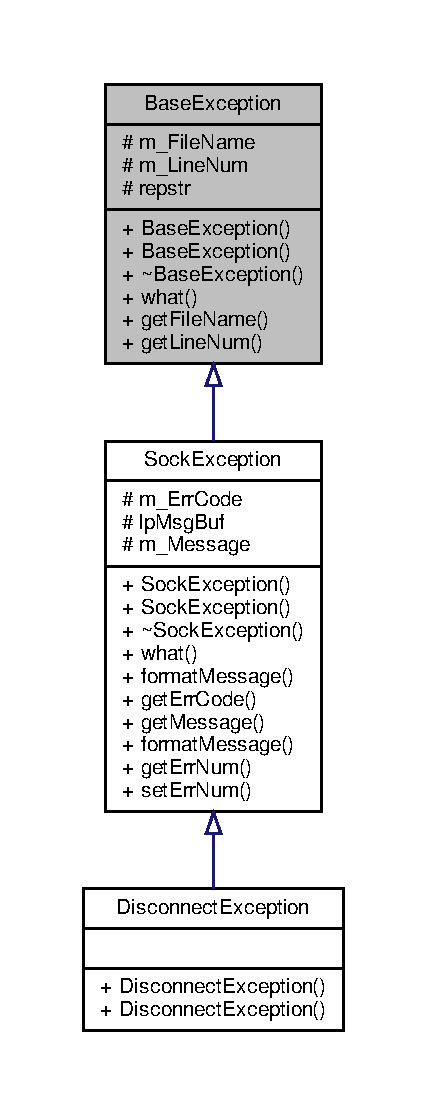
\includegraphics[width=205pt]{classBaseException__inherit__graph}
\end{center}
\end{figure}
\subsection*{Public Member Functions}
\begin{DoxyCompactItemize}
\item 
\hyperlink{group__EXCEPT__GROUP_ga50ebb96feb32366ffc4e992ae5b95e31}{Base\+Exception} (const char $\ast$File\+Name, int Line\+Num)
\item 
\hyperlink{group__EXCEPT__GROUP_ga7b53cdc179f7919010bd7e22c32081e7}{Base\+Exception} (const \hyperlink{classBaseException}{Base\+Exception} \&exp)
\item 
virtual \hyperlink{group__EXCEPT__GROUP_gabc351b149be47d3e078dc04b9b5c8891}{$\sim$\+Base\+Exception} ()
\item 
virtual const char $\ast$ \hyperlink{group__EXCEPT__GROUP_gaf092dd6587491cd7a8cdd987597b1018}{what} ()
\item 
const char $\ast$ \hyperlink{group__EXCEPT__GROUP_gaeea140646898fbe7642cd2dc13b2b22c}{get\+File\+Name} ()
\item 
int \hyperlink{group__EXCEPT__GROUP_ga70bef940bbfd7bb2cc50b8150e1bded2}{get\+Line\+Num} ()
\end{DoxyCompactItemize}
\subsection*{Protected Attributes}
\begin{DoxyCompactItemize}
\item 
char \hyperlink{group__EXCEPT__GROUP_gab2b4ea653318d8effd1d4d6d3cdc53d2}{m\+\_\+\+File\+Name} \mbox{[}256\mbox{]}
\begin{DoxyCompactList}\small\item\em Buffer for filename of the exception source. \end{DoxyCompactList}\item 
int \hyperlink{group__EXCEPT__GROUP_ga40bdabd0e0187fc6738ce0c44564da99}{m\+\_\+\+Line\+Num}
\begin{DoxyCompactList}\small\item\em Line number of the exception source. \end{DoxyCompactList}\item 
std\+::string \hyperlink{group__EXCEPT__GROUP_gad3dcd3ea212b160842c33b62955c4ff9}{repstr}
\begin{DoxyCompactList}\small\item\em String for the exception report will be build to. \end{DoxyCompactList}\end{DoxyCompactItemize}


\subsection{Detailed Description}
Base class for socket class library exceptions 

The documentation for this class was generated from the following file\+:\begin{DoxyCompactItemize}
\item 
\hyperlink{BaseException_8h}{Base\+Exception.\+h}\end{DoxyCompactItemize}

\hypertarget{classBoundSocketV4}{}\section{Bound\+Socket\+V4 Class Reference}
\label{classBoundSocketV4}\index{Bound\+Socket\+V4@{Bound\+Socket\+V4}}


Socket bounded to particular port and I\+Pv4 address (end-\/point).  




{\ttfamily \#include $<$Bound\+Socket\+V4.\+h$>$}



Inheritance diagram for Bound\+Socket\+V4\+:\nopagebreak
\begin{figure}[H]
\begin{center}
\leavevmode
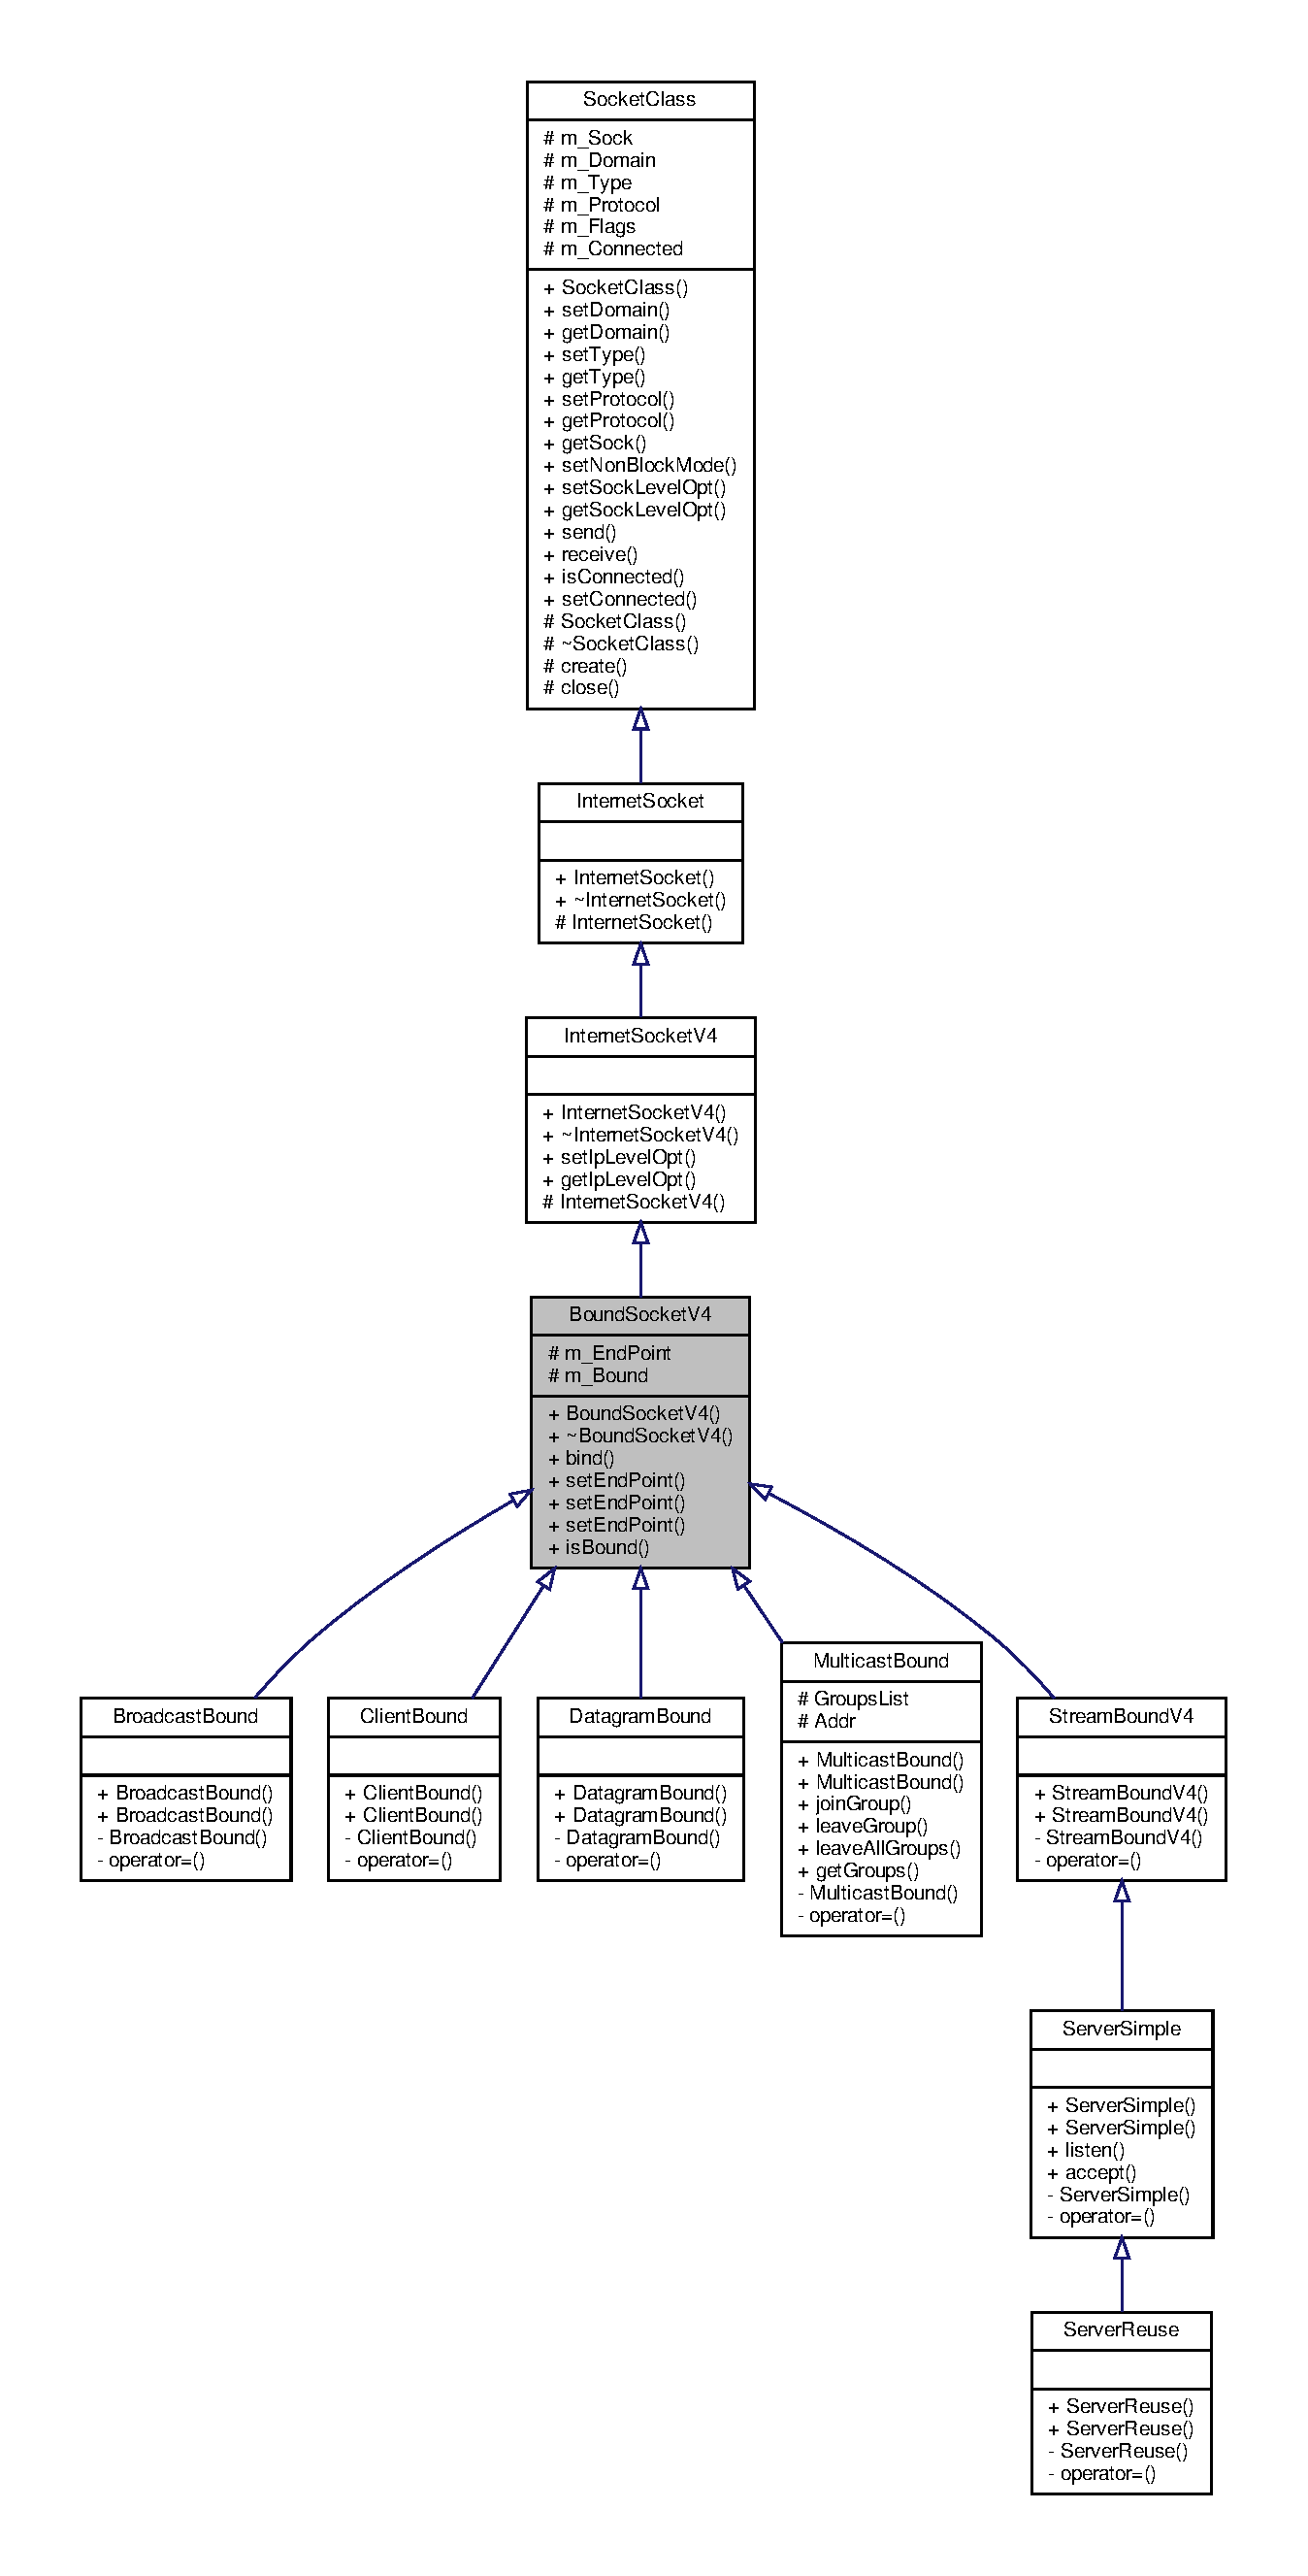
\includegraphics[height=550pt]{classBoundSocketV4__inherit__graph}
\end{center}
\end{figure}
\subsection*{Public Member Functions}
\begin{DoxyCompactItemize}
\item 
\hyperlink{classBoundSocketV4_a6de624ded6ab107a35c5420bacaa75ae}{Bound\+Socket\+V4} ()
\item 
virtual \hyperlink{classBoundSocketV4_a4cdcca1dc8bdcf1af76ac34fe07bc84f}{$\sim$\+Bound\+Socket\+V4} ()
\item 
virtual void \hyperlink{classBoundSocketV4_ad7165f6b77c9c813352179fcf3910b54}{bind} ()
\item 
virtual void \hyperlink{classBoundSocketV4_ac1985788415bf47dd7c91980e5079f1a}{set\+End\+Point} (sockaddr\+\_\+in Addr)
\item 
virtual void \hyperlink{classBoundSocketV4_a908a6e916879fc18585fef69d0518171}{set\+End\+Point} (in\+\_\+addr\+\_\+t Address, short Port)
\item 
virtual void \hyperlink{classBoundSocketV4_a5d3bb922ff5727df01e20782b546714e}{set\+End\+Point} (const char $\ast$Address, short Port)
\item 
bool \hyperlink{classBoundSocketV4_aa7a4ecb65ba394e04763bf486de67d4e}{is\+Bound} ()
\end{DoxyCompactItemize}
\subsection*{Protected Attributes}
\begin{DoxyCompactItemize}
\item 
sockaddr\+\_\+in \hyperlink{classBoundSocketV4_ac19d591b590885f2d34c4b49ba8672db}{m\+\_\+\+End\+Point}
\begin{DoxyCompactList}\small\item\em Socket\textquotesingle{}s bound endpoint. \end{DoxyCompactList}\item 
bool \hyperlink{classBoundSocketV4_a88412526307c31c1843010e5aad30dc7}{m\+\_\+\+Bound}
\begin{DoxyCompactList}\small\item\em Bound status. \end{DoxyCompactList}\end{DoxyCompactItemize}
\subsection*{Additional Inherited Members}


\subsection{Detailed Description}
Socket bounded to particular port and I\+Pv4 address (end-\/point). 

\subsection{Constructor \& Destructor Documentation}
\mbox{\Hypertarget{classBoundSocketV4_a6de624ded6ab107a35c5420bacaa75ae}\label{classBoundSocketV4_a6de624ded6ab107a35c5420bacaa75ae}} 
\index{Bound\+Socket\+V4@{Bound\+Socket\+V4}!Bound\+Socket\+V4@{Bound\+Socket\+V4}}
\index{Bound\+Socket\+V4@{Bound\+Socket\+V4}!Bound\+Socket\+V4@{Bound\+Socket\+V4}}
\subsubsection{\texorpdfstring{Bound\+Socket\+V4()}{BoundSocketV4()}}
{\footnotesize\ttfamily Bound\+Socket\+V4\+::\+Bound\+Socket\+V4 (\begin{DoxyParamCaption}{ }\end{DoxyParamCaption})}

Constructor. Default constructor. \mbox{\Hypertarget{classBoundSocketV4_a4cdcca1dc8bdcf1af76ac34fe07bc84f}\label{classBoundSocketV4_a4cdcca1dc8bdcf1af76ac34fe07bc84f}} 
\index{Bound\+Socket\+V4@{Bound\+Socket\+V4}!````~Bound\+Socket\+V4@{$\sim$\+Bound\+Socket\+V4}}
\index{````~Bound\+Socket\+V4@{$\sim$\+Bound\+Socket\+V4}!Bound\+Socket\+V4@{Bound\+Socket\+V4}}
\subsubsection{\texorpdfstring{$\sim$\+Bound\+Socket\+V4()}{~BoundSocketV4()}}
{\footnotesize\ttfamily virtual Bound\+Socket\+V4\+::$\sim$\+Bound\+Socket\+V4 (\begin{DoxyParamCaption}{ }\end{DoxyParamCaption})\hspace{0.3cm}{\ttfamily [inline]}, {\ttfamily [virtual]}}

Destructor Empty virtual destructor for warning elimination in Eclipse 

\subsection{Member Function Documentation}
\mbox{\Hypertarget{classBoundSocketV4_ad7165f6b77c9c813352179fcf3910b54}\label{classBoundSocketV4_ad7165f6b77c9c813352179fcf3910b54}} 
\index{Bound\+Socket\+V4@{Bound\+Socket\+V4}!bind@{bind}}
\index{bind@{bind}!Bound\+Socket\+V4@{Bound\+Socket\+V4}}
\subsubsection{\texorpdfstring{bind()}{bind()}}
{\footnotesize\ttfamily void Bound\+Socket\+V4\+::bind (\begin{DoxyParamCaption}{ }\end{DoxyParamCaption})\hspace{0.3cm}{\ttfamily [virtual]}}

Bind socket to endpoint. 
\begin{DoxyExceptions}{Exceptions}
{\em Sock\+Exception.} & \\
\hline
\end{DoxyExceptions}
\mbox{\Hypertarget{classBoundSocketV4_aa7a4ecb65ba394e04763bf486de67d4e}\label{classBoundSocketV4_aa7a4ecb65ba394e04763bf486de67d4e}} 
\index{Bound\+Socket\+V4@{Bound\+Socket\+V4}!is\+Bound@{is\+Bound}}
\index{is\+Bound@{is\+Bound}!Bound\+Socket\+V4@{Bound\+Socket\+V4}}
\subsubsection{\texorpdfstring{is\+Bound()}{isBound()}}
{\footnotesize\ttfamily bool Bound\+Socket\+V4\+::is\+Bound (\begin{DoxyParamCaption}{ }\end{DoxyParamCaption})\hspace{0.3cm}{\ttfamily [inline]}}

Is the socket bound already? \begin{DoxyReturn}{Returns}
Bound status. 
\end{DoxyReturn}
\mbox{\Hypertarget{classBoundSocketV4_ac1985788415bf47dd7c91980e5079f1a}\label{classBoundSocketV4_ac1985788415bf47dd7c91980e5079f1a}} 
\index{Bound\+Socket\+V4@{Bound\+Socket\+V4}!set\+End\+Point@{set\+End\+Point}}
\index{set\+End\+Point@{set\+End\+Point}!Bound\+Socket\+V4@{Bound\+Socket\+V4}}
\subsubsection{\texorpdfstring{set\+End\+Point()}{setEndPoint()}\hspace{0.1cm}{\footnotesize\ttfamily [1/3]}}
{\footnotesize\ttfamily virtual void Bound\+Socket\+V4\+::set\+End\+Point (\begin{DoxyParamCaption}\item[{sockaddr\+\_\+in}]{Addr }\end{DoxyParamCaption})\hspace{0.3cm}{\ttfamily [inline]}, {\ttfamily [virtual]}}

Set endpoint for bind the socket. 
\begin{DoxyParams}{Parameters}
{\em Addr} & \+: sockaddr\+\_\+in structure filled with endpoint properties. \\
\hline
\end{DoxyParams}
\mbox{\Hypertarget{classBoundSocketV4_a908a6e916879fc18585fef69d0518171}\label{classBoundSocketV4_a908a6e916879fc18585fef69d0518171}} 
\index{Bound\+Socket\+V4@{Bound\+Socket\+V4}!set\+End\+Point@{set\+End\+Point}}
\index{set\+End\+Point@{set\+End\+Point}!Bound\+Socket\+V4@{Bound\+Socket\+V4}}
\subsubsection{\texorpdfstring{set\+End\+Point()}{setEndPoint()}\hspace{0.1cm}{\footnotesize\ttfamily [2/3]}}
{\footnotesize\ttfamily void Bound\+Socket\+V4\+::set\+End\+Point (\begin{DoxyParamCaption}\item[{in\+\_\+addr\+\_\+t}]{Address,  }\item[{short}]{Port }\end{DoxyParamCaption})\hspace{0.3cm}{\ttfamily [virtual]}}

Set endpoint for bind the socket. 
\begin{DoxyParams}{Parameters}
{\em Address} & \+: I\+Pv4 address in network byte order. \\
\hline
{\em Port} & \+: port number in network byte order. \\
\hline
\end{DoxyParams}
\mbox{\Hypertarget{classBoundSocketV4_a5d3bb922ff5727df01e20782b546714e}\label{classBoundSocketV4_a5d3bb922ff5727df01e20782b546714e}} 
\index{Bound\+Socket\+V4@{Bound\+Socket\+V4}!set\+End\+Point@{set\+End\+Point}}
\index{set\+End\+Point@{set\+End\+Point}!Bound\+Socket\+V4@{Bound\+Socket\+V4}}
\subsubsection{\texorpdfstring{set\+End\+Point()}{setEndPoint()}\hspace{0.1cm}{\footnotesize\ttfamily [3/3]}}
{\footnotesize\ttfamily void Bound\+Socket\+V4\+::set\+End\+Point (\begin{DoxyParamCaption}\item[{const char $\ast$}]{Address,  }\item[{short}]{Port }\end{DoxyParamCaption})\hspace{0.3cm}{\ttfamily [virtual]}}

Set endpoint for bind the socket. 
\begin{DoxyParams}{Parameters}
{\em Address} & \+: I\+Pv4 address in decimal dot notation. \\
\hline
{\em Port} & \+: port number in network byte order. \\
\hline
\end{DoxyParams}


\subsection{Member Data Documentation}
\mbox{\Hypertarget{classBoundSocketV4_a88412526307c31c1843010e5aad30dc7}\label{classBoundSocketV4_a88412526307c31c1843010e5aad30dc7}} 
\index{Bound\+Socket\+V4@{Bound\+Socket\+V4}!m\+\_\+\+Bound@{m\+\_\+\+Bound}}
\index{m\+\_\+\+Bound@{m\+\_\+\+Bound}!Bound\+Socket\+V4@{Bound\+Socket\+V4}}
\subsubsection{\texorpdfstring{m\+\_\+\+Bound}{m\_Bound}}
{\footnotesize\ttfamily bool Bound\+Socket\+V4\+::m\+\_\+\+Bound\hspace{0.3cm}{\ttfamily [protected]}}



Bound status. 

\mbox{\Hypertarget{classBoundSocketV4_ac19d591b590885f2d34c4b49ba8672db}\label{classBoundSocketV4_ac19d591b590885f2d34c4b49ba8672db}} 
\index{Bound\+Socket\+V4@{Bound\+Socket\+V4}!m\+\_\+\+End\+Point@{m\+\_\+\+End\+Point}}
\index{m\+\_\+\+End\+Point@{m\+\_\+\+End\+Point}!Bound\+Socket\+V4@{Bound\+Socket\+V4}}
\subsubsection{\texorpdfstring{m\+\_\+\+End\+Point}{m\_EndPoint}}
{\footnotesize\ttfamily sockaddr\+\_\+in Bound\+Socket\+V4\+::m\+\_\+\+End\+Point\hspace{0.3cm}{\ttfamily [protected]}}



Socket\textquotesingle{}s bound endpoint. 



The documentation for this class was generated from the following files\+:\begin{DoxyCompactItemize}
\item 
\hyperlink{BoundSocketV4_8h}{Bound\+Socket\+V4.\+h}\item 
\hyperlink{BoundSocketV4_8cpp}{Bound\+Socket\+V4.\+cpp}\end{DoxyCompactItemize}

\hypertarget{classBoundSocketV6}{}\section{Bound\+Socket\+V6 Class Reference}
\label{classBoundSocketV6}\index{Bound\+Socket\+V6@{Bound\+Socket\+V6}}


Socket bounded to particular port and I\+Pv6 address (end-\/point).  




{\ttfamily \#include $<$Bound\+Socket\+V6.\+h$>$}



Inheritance diagram for Bound\+Socket\+V6\+:\nopagebreak
\begin{figure}[H]
\begin{center}
\leavevmode
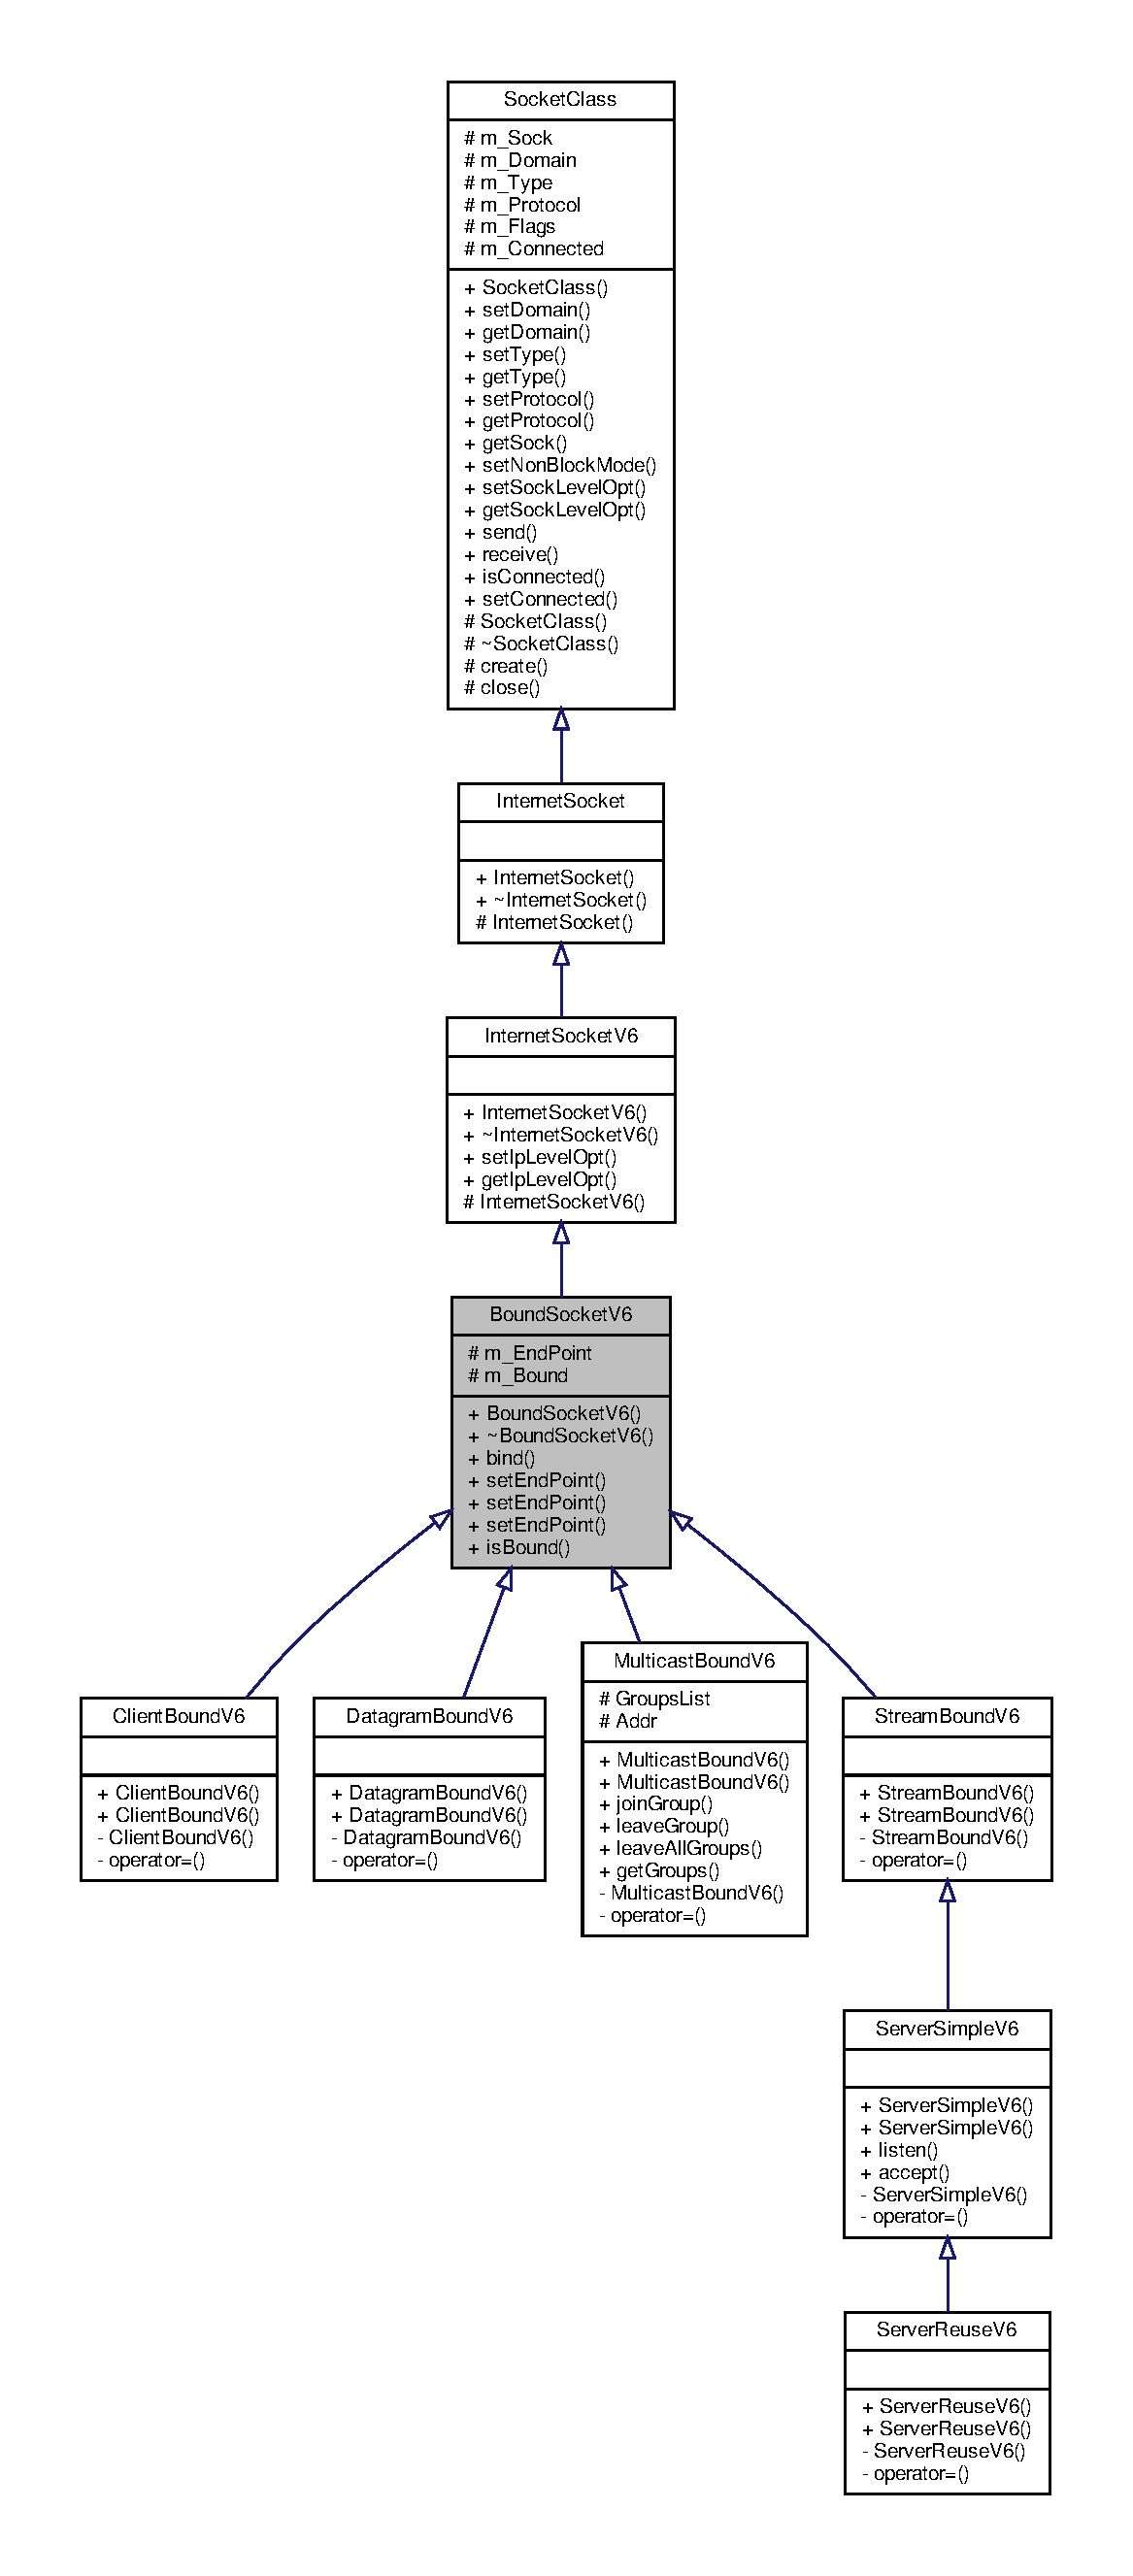
\includegraphics[height=550pt]{classBoundSocketV6__inherit__graph}
\end{center}
\end{figure}
\subsection*{Public Member Functions}
\begin{DoxyCompactItemize}
\item 
\hyperlink{classBoundSocketV6_a99bee564490f6efa36fe13355adcb7cc}{Bound\+Socket\+V6} ()
\item 
virtual \hyperlink{classBoundSocketV6_ac1c31ca5c4be106325146f76af312144}{$\sim$\+Bound\+Socket\+V6} ()
\item 
virtual void \hyperlink{classBoundSocketV6_a76ed837cd1fb36bbc1383f5e7e381095}{bind} ()
\item 
virtual void \hyperlink{classBoundSocketV6_a9f16093436c0325253bbb4069bffce0d}{set\+End\+Point} (sockaddr\+\_\+in6 Addr)
\item 
virtual void \hyperlink{classBoundSocketV6_a3bcb3acaa01f814957b5dc3233cdb0c9}{set\+End\+Point} (in6\+\_\+addr Address, short Port)
\item 
virtual void \hyperlink{classBoundSocketV6_a183ca4435804e6d1ea616c8c74e26e46}{set\+End\+Point} (const char $\ast$Address, short Port)
\item 
bool \hyperlink{classBoundSocketV6_a2a29edc5ad339f83b06bdbc413d949b2}{is\+Bound} ()
\end{DoxyCompactItemize}
\subsection*{Protected Attributes}
\begin{DoxyCompactItemize}
\item 
sockaddr\+\_\+in6 \hyperlink{classBoundSocketV6_abf6063eee350425ae5a105200be62df0}{m\+\_\+\+End\+Point}
\begin{DoxyCompactList}\small\item\em Socket\textquotesingle{}s bound endpoint. \end{DoxyCompactList}\item 
bool \hyperlink{classBoundSocketV6_a0f09faafc821fe3ebe890821d1b4cb10}{m\+\_\+\+Bound}
\begin{DoxyCompactList}\small\item\em Bound status. \end{DoxyCompactList}\end{DoxyCompactItemize}
\subsection*{Additional Inherited Members}


\subsection{Detailed Description}
Socket bounded to particular port and I\+Pv6 address (end-\/point). 

\subsection{Constructor \& Destructor Documentation}
\mbox{\Hypertarget{classBoundSocketV6_a99bee564490f6efa36fe13355adcb7cc}\label{classBoundSocketV6_a99bee564490f6efa36fe13355adcb7cc}} 
\index{Bound\+Socket\+V6@{Bound\+Socket\+V6}!Bound\+Socket\+V6@{Bound\+Socket\+V6}}
\index{Bound\+Socket\+V6@{Bound\+Socket\+V6}!Bound\+Socket\+V6@{Bound\+Socket\+V6}}
\subsubsection{\texorpdfstring{Bound\+Socket\+V6()}{BoundSocketV6()}}
{\footnotesize\ttfamily Bound\+Socket\+V6\+::\+Bound\+Socket\+V6 (\begin{DoxyParamCaption}{ }\end{DoxyParamCaption})}

Constructor. Default constructor. \mbox{\Hypertarget{classBoundSocketV6_ac1c31ca5c4be106325146f76af312144}\label{classBoundSocketV6_ac1c31ca5c4be106325146f76af312144}} 
\index{Bound\+Socket\+V6@{Bound\+Socket\+V6}!````~Bound\+Socket\+V6@{$\sim$\+Bound\+Socket\+V6}}
\index{````~Bound\+Socket\+V6@{$\sim$\+Bound\+Socket\+V6}!Bound\+Socket\+V6@{Bound\+Socket\+V6}}
\subsubsection{\texorpdfstring{$\sim$\+Bound\+Socket\+V6()}{~BoundSocketV6()}}
{\footnotesize\ttfamily virtual Bound\+Socket\+V6\+::$\sim$\+Bound\+Socket\+V6 (\begin{DoxyParamCaption}{ }\end{DoxyParamCaption})\hspace{0.3cm}{\ttfamily [inline]}, {\ttfamily [virtual]}}

Destructor Empty virtual destructor for warning elimination in Eclipse 

\subsection{Member Function Documentation}
\mbox{\Hypertarget{classBoundSocketV6_a76ed837cd1fb36bbc1383f5e7e381095}\label{classBoundSocketV6_a76ed837cd1fb36bbc1383f5e7e381095}} 
\index{Bound\+Socket\+V6@{Bound\+Socket\+V6}!bind@{bind}}
\index{bind@{bind}!Bound\+Socket\+V6@{Bound\+Socket\+V6}}
\subsubsection{\texorpdfstring{bind()}{bind()}}
{\footnotesize\ttfamily void Bound\+Socket\+V6\+::bind (\begin{DoxyParamCaption}{ }\end{DoxyParamCaption})\hspace{0.3cm}{\ttfamily [virtual]}}

Bind socket to endpoint. 
\begin{DoxyExceptions}{Exceptions}
{\em Sock\+Exception.} & \\
\hline
\end{DoxyExceptions}
\mbox{\Hypertarget{classBoundSocketV6_a2a29edc5ad339f83b06bdbc413d949b2}\label{classBoundSocketV6_a2a29edc5ad339f83b06bdbc413d949b2}} 
\index{Bound\+Socket\+V6@{Bound\+Socket\+V6}!is\+Bound@{is\+Bound}}
\index{is\+Bound@{is\+Bound}!Bound\+Socket\+V6@{Bound\+Socket\+V6}}
\subsubsection{\texorpdfstring{is\+Bound()}{isBound()}}
{\footnotesize\ttfamily bool Bound\+Socket\+V6\+::is\+Bound (\begin{DoxyParamCaption}{ }\end{DoxyParamCaption})\hspace{0.3cm}{\ttfamily [inline]}}

Is the socket bound already? \begin{DoxyReturn}{Returns}
Bound status. 
\end{DoxyReturn}
\mbox{\Hypertarget{classBoundSocketV6_a9f16093436c0325253bbb4069bffce0d}\label{classBoundSocketV6_a9f16093436c0325253bbb4069bffce0d}} 
\index{Bound\+Socket\+V6@{Bound\+Socket\+V6}!set\+End\+Point@{set\+End\+Point}}
\index{set\+End\+Point@{set\+End\+Point}!Bound\+Socket\+V6@{Bound\+Socket\+V6}}
\subsubsection{\texorpdfstring{set\+End\+Point()}{setEndPoint()}\hspace{0.1cm}{\footnotesize\ttfamily [1/3]}}
{\footnotesize\ttfamily virtual void Bound\+Socket\+V6\+::set\+End\+Point (\begin{DoxyParamCaption}\item[{sockaddr\+\_\+in6}]{Addr }\end{DoxyParamCaption})\hspace{0.3cm}{\ttfamily [inline]}, {\ttfamily [virtual]}}

Set endpoint for bind the socket. 
\begin{DoxyParams}{Parameters}
{\em Addr} & \+: sockaddr\+\_\+in6 structure filled with endpoint properties. \\
\hline
\end{DoxyParams}
\mbox{\Hypertarget{classBoundSocketV6_a3bcb3acaa01f814957b5dc3233cdb0c9}\label{classBoundSocketV6_a3bcb3acaa01f814957b5dc3233cdb0c9}} 
\index{Bound\+Socket\+V6@{Bound\+Socket\+V6}!set\+End\+Point@{set\+End\+Point}}
\index{set\+End\+Point@{set\+End\+Point}!Bound\+Socket\+V6@{Bound\+Socket\+V6}}
\subsubsection{\texorpdfstring{set\+End\+Point()}{setEndPoint()}\hspace{0.1cm}{\footnotesize\ttfamily [2/3]}}
{\footnotesize\ttfamily void Bound\+Socket\+V6\+::set\+End\+Point (\begin{DoxyParamCaption}\item[{in6\+\_\+addr}]{Address,  }\item[{short}]{Port }\end{DoxyParamCaption})\hspace{0.3cm}{\ttfamily [virtual]}}

Set endpoint for bind the socket. 
\begin{DoxyParams}{Parameters}
{\em Address} & \+: I\+Pv6 address in network byte order. \\
\hline
{\em Port} & \+: port number in network byte order. \\
\hline
\end{DoxyParams}
\mbox{\Hypertarget{classBoundSocketV6_a183ca4435804e6d1ea616c8c74e26e46}\label{classBoundSocketV6_a183ca4435804e6d1ea616c8c74e26e46}} 
\index{Bound\+Socket\+V6@{Bound\+Socket\+V6}!set\+End\+Point@{set\+End\+Point}}
\index{set\+End\+Point@{set\+End\+Point}!Bound\+Socket\+V6@{Bound\+Socket\+V6}}
\subsubsection{\texorpdfstring{set\+End\+Point()}{setEndPoint()}\hspace{0.1cm}{\footnotesize\ttfamily [3/3]}}
{\footnotesize\ttfamily void Bound\+Socket\+V6\+::set\+End\+Point (\begin{DoxyParamCaption}\item[{const char $\ast$}]{Address,  }\item[{short}]{Port }\end{DoxyParamCaption})\hspace{0.3cm}{\ttfamily [virtual]}}

Set endpoint for bind the socket. 
\begin{DoxyParams}{Parameters}
{\em Address} & \+: I\+Pv6 address textual notation. \\
\hline
{\em Port} & \+: port number in network byte order. \\
\hline
\end{DoxyParams}


\subsection{Member Data Documentation}
\mbox{\Hypertarget{classBoundSocketV6_a0f09faafc821fe3ebe890821d1b4cb10}\label{classBoundSocketV6_a0f09faafc821fe3ebe890821d1b4cb10}} 
\index{Bound\+Socket\+V6@{Bound\+Socket\+V6}!m\+\_\+\+Bound@{m\+\_\+\+Bound}}
\index{m\+\_\+\+Bound@{m\+\_\+\+Bound}!Bound\+Socket\+V6@{Bound\+Socket\+V6}}
\subsubsection{\texorpdfstring{m\+\_\+\+Bound}{m\_Bound}}
{\footnotesize\ttfamily bool Bound\+Socket\+V6\+::m\+\_\+\+Bound\hspace{0.3cm}{\ttfamily [protected]}}



Bound status. 

\mbox{\Hypertarget{classBoundSocketV6_abf6063eee350425ae5a105200be62df0}\label{classBoundSocketV6_abf6063eee350425ae5a105200be62df0}} 
\index{Bound\+Socket\+V6@{Bound\+Socket\+V6}!m\+\_\+\+End\+Point@{m\+\_\+\+End\+Point}}
\index{m\+\_\+\+End\+Point@{m\+\_\+\+End\+Point}!Bound\+Socket\+V6@{Bound\+Socket\+V6}}
\subsubsection{\texorpdfstring{m\+\_\+\+End\+Point}{m\_EndPoint}}
{\footnotesize\ttfamily sockaddr\+\_\+in6 Bound\+Socket\+V6\+::m\+\_\+\+End\+Point\hspace{0.3cm}{\ttfamily [protected]}}



Socket\textquotesingle{}s bound endpoint. 



The documentation for this class was generated from the following files\+:\begin{DoxyCompactItemize}
\item 
\hyperlink{BoundSocketV6_8h}{Bound\+Socket\+V6.\+h}\item 
\hyperlink{BoundSocketV6_8cpp}{Bound\+Socket\+V6.\+cpp}\end{DoxyCompactItemize}

\hypertarget{classBroadcastBound}{}\section{Broadcast\+Bound Class Reference}
\label{classBroadcastBound}\index{Broadcast\+Bound@{Broadcast\+Bound}}


Bounded socket with broadcast capabilities.  




{\ttfamily \#include $<$Broadcast\+Bound.\+h$>$}



Inheritance diagram for Broadcast\+Bound\+:\nopagebreak
\begin{figure}[H]
\begin{center}
\leavevmode
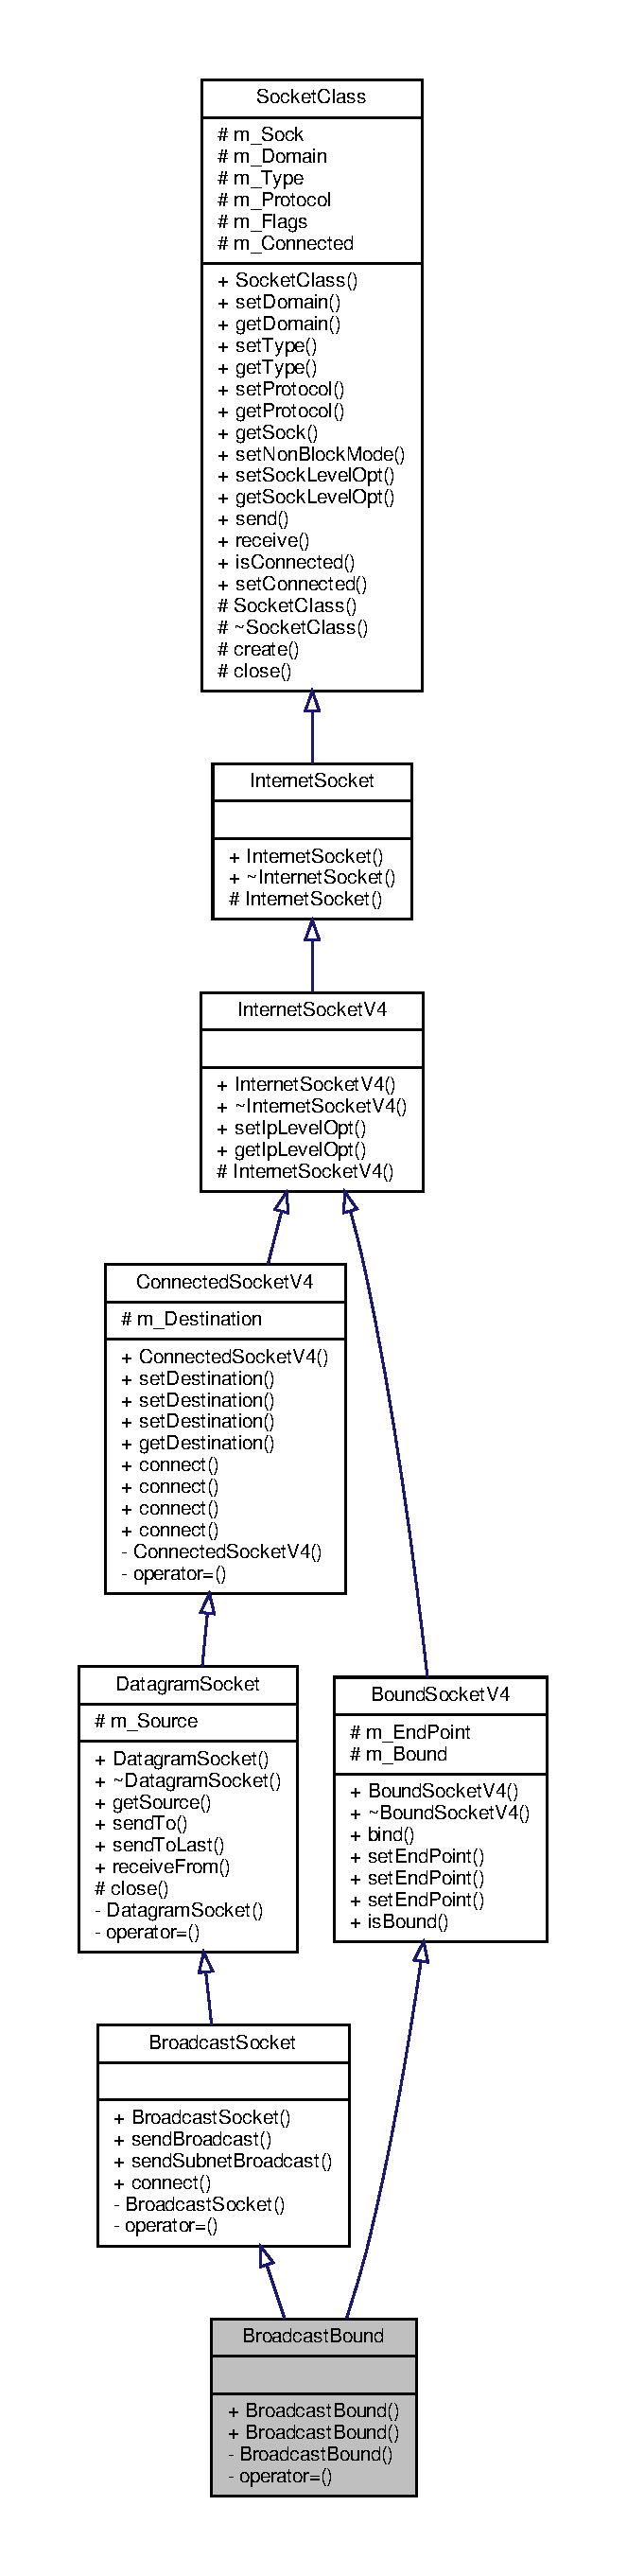
\includegraphics[height=550pt]{classBroadcastBound__inherit__graph}
\end{center}
\end{figure}
\subsection*{Public Member Functions}
\begin{DoxyCompactItemize}
\item 
\hyperlink{classBroadcastBound_a22bb046de1f37baeb7c912c6383365f1}{Broadcast\+Bound} (short Port, in\+\_\+addr\+\_\+t Address=I\+N\+A\+D\+D\+R\+\_\+\+A\+NY)
\item 
\hyperlink{classBroadcastBound_a77bafc8d719b40f9e8de10ca8f9969c1}{Broadcast\+Bound} (short Port, const char $\ast$Address)
\end{DoxyCompactItemize}
\subsection*{Private Member Functions}
\begin{DoxyCompactItemize}
\item 
\hyperlink{classBroadcastBound_a154c02a5f59ba620ac0b09431a1fae07}{Broadcast\+Bound} (\hyperlink{classBroadcastBound}{Broadcast\+Bound} \&d)
\item 
\hyperlink{classBroadcastBound}{Broadcast\+Bound} \& \hyperlink{classBroadcastBound_ad87e73f7cba821eea8f111c64868356b}{operator=} (\hyperlink{classBroadcastBound}{Broadcast\+Bound} \&d)
\end{DoxyCompactItemize}
\subsection*{Additional Inherited Members}


\subsection{Detailed Description}
Bounded socket with broadcast capabilities. 

\subsection{Constructor \& Destructor Documentation}
\mbox{\Hypertarget{classBroadcastBound_a22bb046de1f37baeb7c912c6383365f1}\label{classBroadcastBound_a22bb046de1f37baeb7c912c6383365f1}} 
\index{Broadcast\+Bound@{Broadcast\+Bound}!Broadcast\+Bound@{Broadcast\+Bound}}
\index{Broadcast\+Bound@{Broadcast\+Bound}!Broadcast\+Bound@{Broadcast\+Bound}}
\subsubsection{\texorpdfstring{Broadcast\+Bound()}{BroadcastBound()}\hspace{0.1cm}{\footnotesize\ttfamily [1/3]}}
{\footnotesize\ttfamily Broadcast\+Bound\+::\+Broadcast\+Bound (\begin{DoxyParamCaption}\item[{short}]{Port,  }\item[{in\+\_\+addr\+\_\+t}]{Address = {\ttfamily INADDR\+\_\+ANY} }\end{DoxyParamCaption})}

Constructor. 
\begin{DoxyParams}{Parameters}
{\em Port} & \+: port number for bind in network byte order. \\
\hline
{\em Address} & \+: address for bind in network byte order. \\
\hline
\end{DoxyParams}

\begin{DoxyExceptions}{Exceptions}
{\em Sock\+Exception.} & \\
\hline
\end{DoxyExceptions}
\mbox{\Hypertarget{classBroadcastBound_a77bafc8d719b40f9e8de10ca8f9969c1}\label{classBroadcastBound_a77bafc8d719b40f9e8de10ca8f9969c1}} 
\index{Broadcast\+Bound@{Broadcast\+Bound}!Broadcast\+Bound@{Broadcast\+Bound}}
\index{Broadcast\+Bound@{Broadcast\+Bound}!Broadcast\+Bound@{Broadcast\+Bound}}
\subsubsection{\texorpdfstring{Broadcast\+Bound()}{BroadcastBound()}\hspace{0.1cm}{\footnotesize\ttfamily [2/3]}}
{\footnotesize\ttfamily Broadcast\+Bound\+::\+Broadcast\+Bound (\begin{DoxyParamCaption}\item[{short}]{Port,  }\item[{const char $\ast$}]{Address }\end{DoxyParamCaption})}

Constructor. 
\begin{DoxyParams}{Parameters}
{\em Port} & \+: port number for bind in network byte order. \\
\hline
{\em Address} & \+: address for bind in decimal dot notation. \\
\hline
\end{DoxyParams}

\begin{DoxyExceptions}{Exceptions}
{\em Sock\+Exception.} & \\
\hline
\end{DoxyExceptions}
\mbox{\Hypertarget{classBroadcastBound_a154c02a5f59ba620ac0b09431a1fae07}\label{classBroadcastBound_a154c02a5f59ba620ac0b09431a1fae07}} 
\index{Broadcast\+Bound@{Broadcast\+Bound}!Broadcast\+Bound@{Broadcast\+Bound}}
\index{Broadcast\+Bound@{Broadcast\+Bound}!Broadcast\+Bound@{Broadcast\+Bound}}
\subsubsection{\texorpdfstring{Broadcast\+Bound()}{BroadcastBound()}\hspace{0.1cm}{\footnotesize\ttfamily [3/3]}}
{\footnotesize\ttfamily Broadcast\+Bound\+::\+Broadcast\+Bound (\begin{DoxyParamCaption}\item[{\hyperlink{classBroadcastBound}{Broadcast\+Bound} \&}]{d }\end{DoxyParamCaption})\hspace{0.3cm}{\ttfamily [private]}}

Copy constructor. Makes the class uncopyable. 

\subsection{Member Function Documentation}
\mbox{\Hypertarget{classBroadcastBound_ad87e73f7cba821eea8f111c64868356b}\label{classBroadcastBound_ad87e73f7cba821eea8f111c64868356b}} 
\index{Broadcast\+Bound@{Broadcast\+Bound}!operator=@{operator=}}
\index{operator=@{operator=}!Broadcast\+Bound@{Broadcast\+Bound}}
\subsubsection{\texorpdfstring{operator=()}{operator=()}}
{\footnotesize\ttfamily \hyperlink{classBroadcastBound}{Broadcast\+Bound}\& Broadcast\+Bound\+::operator= (\begin{DoxyParamCaption}\item[{\hyperlink{classBroadcastBound}{Broadcast\+Bound} \&}]{d }\end{DoxyParamCaption})\hspace{0.3cm}{\ttfamily [private]}}

Operator assign. Makes the class uncopyable. 

The documentation for this class was generated from the following files\+:\begin{DoxyCompactItemize}
\item 
\hyperlink{BroadcastBound_8h}{Broadcast\+Bound.\+h}\item 
\hyperlink{BroadcastBound_8cpp}{Broadcast\+Bound.\+cpp}\end{DoxyCompactItemize}

\hypertarget{classBroadcastSocket}{}\section{Broadcast\+Socket Class Reference}
\label{classBroadcastSocket}\index{Broadcast\+Socket@{Broadcast\+Socket}}


Broadcast socket class.  




{\ttfamily \#include $<$Broadcast\+Socket.\+h$>$}



Inheritance diagram for Broadcast\+Socket\+:\nopagebreak
\begin{figure}[H]
\begin{center}
\leavevmode
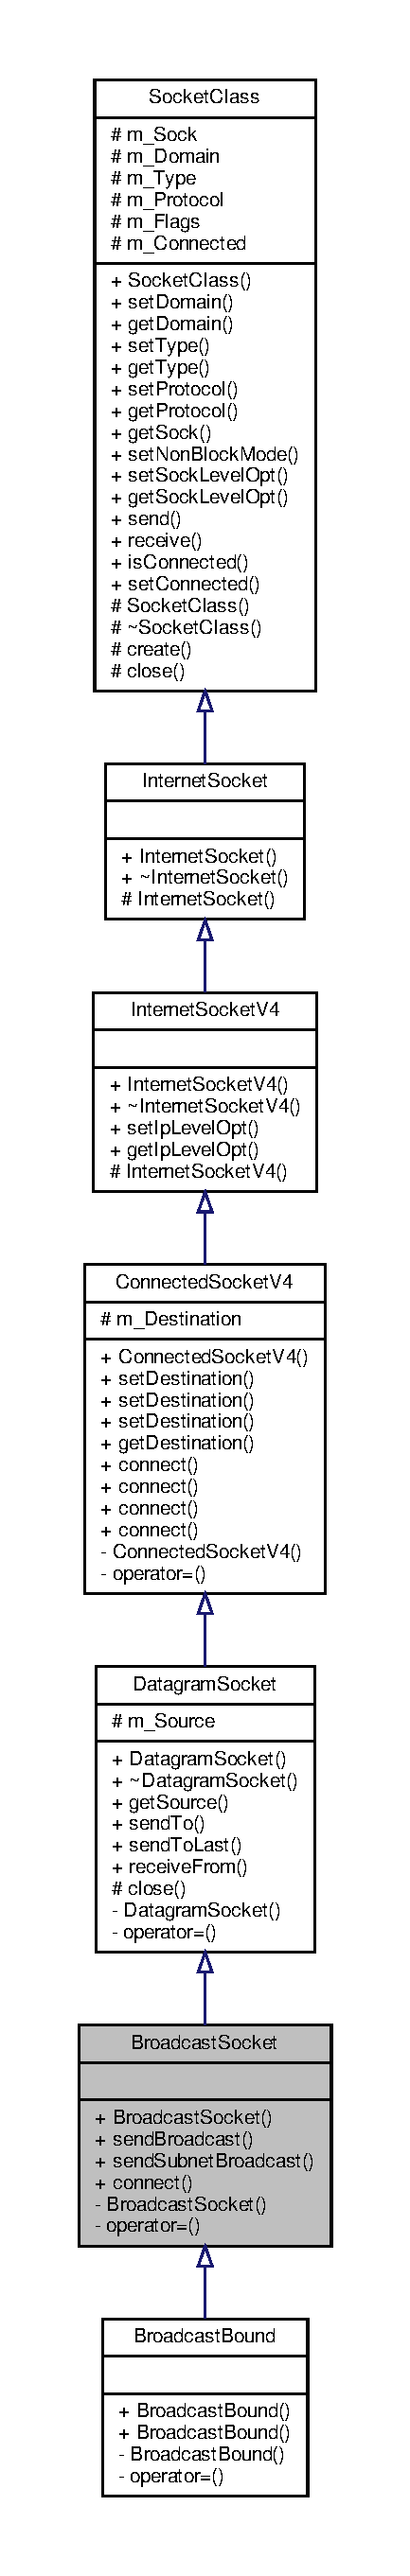
\includegraphics[height=550pt]{classBroadcastSocket__inherit__graph}
\end{center}
\end{figure}
\subsection*{Public Member Functions}
\begin{DoxyCompactItemize}
\item 
\hyperlink{classBroadcastSocket_a1d24d481f9947743896280d1f1c2cc8a}{Broadcast\+Socket} ()
\item 
int \hyperlink{classBroadcastSocket_a5e8f0ca3c127e9e5be5b6c994feb46ad}{send\+Broadcast} (short Port, const void $\ast$Buffer, size\+\_\+t Length, int Flags=0)
\item 
int \hyperlink{classBroadcastSocket_a184bc48d22498cb3a8c8de927cbae917}{send\+Subnet\+Broadcast} (in\+\_\+addr\+\_\+t Addr, short Port, const void $\ast$Buffer, size\+\_\+t Length, int Flags=0)
\item 
virtual void \hyperlink{classBroadcastSocket_a330f3448f2c53eef77af683cfd94eafd}{connect} ()
\end{DoxyCompactItemize}
\subsection*{Private Member Functions}
\begin{DoxyCompactItemize}
\item 
\hyperlink{classBroadcastSocket_a3f141e2a8c35c074ae18e8f6da272189}{Broadcast\+Socket} (\hyperlink{classBroadcastSocket}{Broadcast\+Socket} \&b)
\item 
\hyperlink{classBroadcastSocket}{Broadcast\+Socket} \& \hyperlink{classBroadcastSocket_adf79ba7c618dd87731908773e77bea8b}{operator=} (\hyperlink{classBroadcastSocket}{Broadcast\+Socket} \&b)
\end{DoxyCompactItemize}
\subsection*{Additional Inherited Members}


\subsection{Detailed Description}
Broadcast socket class. 

\subsection{Constructor \& Destructor Documentation}
\mbox{\Hypertarget{classBroadcastSocket_a1d24d481f9947743896280d1f1c2cc8a}\label{classBroadcastSocket_a1d24d481f9947743896280d1f1c2cc8a}} 
\index{Broadcast\+Socket@{Broadcast\+Socket}!Broadcast\+Socket@{Broadcast\+Socket}}
\index{Broadcast\+Socket@{Broadcast\+Socket}!Broadcast\+Socket@{Broadcast\+Socket}}
\subsubsection{\texorpdfstring{Broadcast\+Socket()}{BroadcastSocket()}\hspace{0.1cm}{\footnotesize\ttfamily [1/2]}}
{\footnotesize\ttfamily Broadcast\+Socket\+::\+Broadcast\+Socket (\begin{DoxyParamCaption}{ }\end{DoxyParamCaption})}

Constructor. Default constructor. 
\begin{DoxyExceptions}{Exceptions}
{\em Sock\+Exception.} & \\
\hline
\end{DoxyExceptions}
\mbox{\Hypertarget{classBroadcastSocket_a3f141e2a8c35c074ae18e8f6da272189}\label{classBroadcastSocket_a3f141e2a8c35c074ae18e8f6da272189}} 
\index{Broadcast\+Socket@{Broadcast\+Socket}!Broadcast\+Socket@{Broadcast\+Socket}}
\index{Broadcast\+Socket@{Broadcast\+Socket}!Broadcast\+Socket@{Broadcast\+Socket}}
\subsubsection{\texorpdfstring{Broadcast\+Socket()}{BroadcastSocket()}\hspace{0.1cm}{\footnotesize\ttfamily [2/2]}}
{\footnotesize\ttfamily Broadcast\+Socket\+::\+Broadcast\+Socket (\begin{DoxyParamCaption}\item[{\hyperlink{classBroadcastSocket}{Broadcast\+Socket} \&}]{b }\end{DoxyParamCaption})\hspace{0.3cm}{\ttfamily [private]}}

Copy constructor. Makes the class uncopyable. 

\subsection{Member Function Documentation}
\mbox{\Hypertarget{classBroadcastSocket_a330f3448f2c53eef77af683cfd94eafd}\label{classBroadcastSocket_a330f3448f2c53eef77af683cfd94eafd}} 
\index{Broadcast\+Socket@{Broadcast\+Socket}!connect@{connect}}
\index{connect@{connect}!Broadcast\+Socket@{Broadcast\+Socket}}
\subsubsection{\texorpdfstring{connect()}{connect()}}
{\footnotesize\ttfamily virtual void Broadcast\+Socket\+::connect (\begin{DoxyParamCaption}{ }\end{DoxyParamCaption})\hspace{0.3cm}{\ttfamily [inline]}, {\ttfamily [virtual]}}

Connect the socket. Implements pure virtual function of base class. Has no meaning for this particular class. 
\begin{DoxyExceptions}{Exceptions}
{\em Sock\+Exception.} & \\
\hline
\end{DoxyExceptions}


Reimplemented from \hyperlink{classConnectedSocketV4_a034d0c949fa1a0f14c136f839915d1a4}{Connected\+Socket\+V4}.

\mbox{\Hypertarget{classBroadcastSocket_adf79ba7c618dd87731908773e77bea8b}\label{classBroadcastSocket_adf79ba7c618dd87731908773e77bea8b}} 
\index{Broadcast\+Socket@{Broadcast\+Socket}!operator=@{operator=}}
\index{operator=@{operator=}!Broadcast\+Socket@{Broadcast\+Socket}}
\subsubsection{\texorpdfstring{operator=()}{operator=()}}
{\footnotesize\ttfamily \hyperlink{classBroadcastSocket}{Broadcast\+Socket}\& Broadcast\+Socket\+::operator= (\begin{DoxyParamCaption}\item[{\hyperlink{classBroadcastSocket}{Broadcast\+Socket} \&}]{b }\end{DoxyParamCaption})\hspace{0.3cm}{\ttfamily [private]}}

Operator assign. Makes the class uncopyable. \mbox{\Hypertarget{classBroadcastSocket_a5e8f0ca3c127e9e5be5b6c994feb46ad}\label{classBroadcastSocket_a5e8f0ca3c127e9e5be5b6c994feb46ad}} 
\index{Broadcast\+Socket@{Broadcast\+Socket}!send\+Broadcast@{send\+Broadcast}}
\index{send\+Broadcast@{send\+Broadcast}!Broadcast\+Socket@{Broadcast\+Socket}}
\subsubsection{\texorpdfstring{send\+Broadcast()}{sendBroadcast()}}
{\footnotesize\ttfamily int Broadcast\+Socket\+::send\+Broadcast (\begin{DoxyParamCaption}\item[{short}]{Port,  }\item[{const void $\ast$}]{Buffer,  }\item[{size\+\_\+t}]{Length,  }\item[{int}]{Flags = {\ttfamily 0} }\end{DoxyParamCaption})\hspace{0.3cm}{\ttfamily [inline]}}

Send broadcast. 
\begin{DoxyParams}{Parameters}
{\em Port} & \+: destination port in network byte order. \\
\hline
{\em Buffer} & \+: data to send. \\
\hline
{\em Length} & \+: amount of the data. \\
\hline
{\em Flags} & \+: flags, default value -\/ 0. \\
\hline
\end{DoxyParams}

\begin{DoxyExceptions}{Exceptions}
{\em Sock\+Exception.} & \\
\hline
\end{DoxyExceptions}
\mbox{\Hypertarget{classBroadcastSocket_a184bc48d22498cb3a8c8de927cbae917}\label{classBroadcastSocket_a184bc48d22498cb3a8c8de927cbae917}} 
\index{Broadcast\+Socket@{Broadcast\+Socket}!send\+Subnet\+Broadcast@{send\+Subnet\+Broadcast}}
\index{send\+Subnet\+Broadcast@{send\+Subnet\+Broadcast}!Broadcast\+Socket@{Broadcast\+Socket}}
\subsubsection{\texorpdfstring{send\+Subnet\+Broadcast()}{sendSubnetBroadcast()}}
{\footnotesize\ttfamily int Broadcast\+Socket\+::send\+Subnet\+Broadcast (\begin{DoxyParamCaption}\item[{in\+\_\+addr\+\_\+t}]{Addr,  }\item[{short}]{Port,  }\item[{const void $\ast$}]{Buffer,  }\item[{size\+\_\+t}]{Length,  }\item[{int}]{Flags = {\ttfamily 0} }\end{DoxyParamCaption})\hspace{0.3cm}{\ttfamily [inline]}}

Send subnet broadcast. 
\begin{DoxyParams}{Parameters}
{\em Addr} & \+: subnet address in network byte order. \\
\hline
{\em Port} & \+: destination port in network byte order. \\
\hline
{\em Buffer} & \+: data to send. \\
\hline
{\em Length} & \+: amount of the data. \\
\hline
{\em Flags} & \+: flags, default value -\/ 0. \\
\hline
\end{DoxyParams}

\begin{DoxyExceptions}{Exceptions}
{\em Sock\+Exception.} & \\
\hline
\end{DoxyExceptions}


The documentation for this class was generated from the following files\+:\begin{DoxyCompactItemize}
\item 
\hyperlink{BroadcastSocket_8h}{Broadcast\+Socket.\+h}\item 
\hyperlink{BroadcastSocket_8cpp}{Broadcast\+Socket.\+cpp}\end{DoxyCompactItemize}

\hypertarget{classClientBound}{}\section{Client\+Bound Class Reference}
\label{classClientBound}\index{Client\+Bound@{Client\+Bound}}


Client socket bound to specified port and address.  




{\ttfamily \#include $<$Client\+Bound.\+h$>$}



Inheritance diagram for Client\+Bound\+:\nopagebreak
\begin{figure}[H]
\begin{center}
\leavevmode
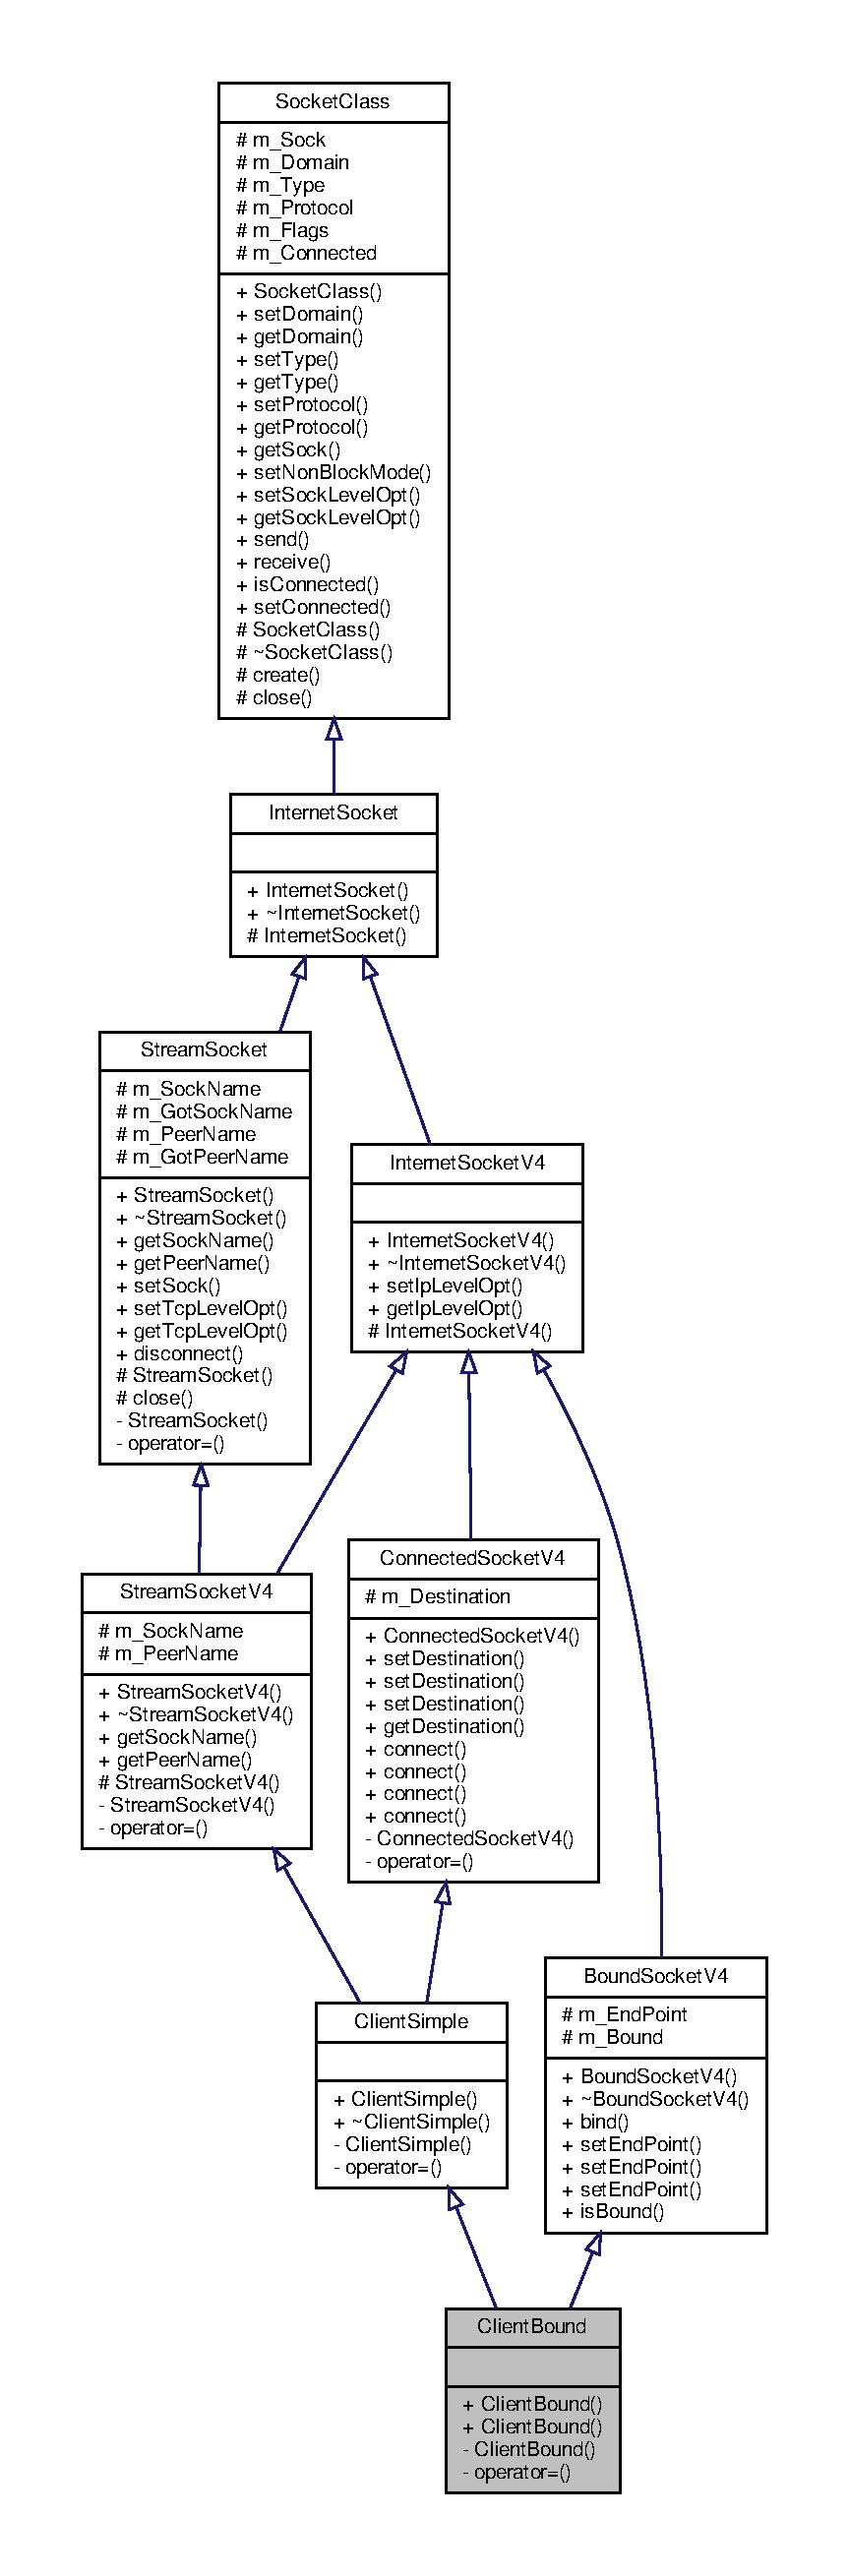
\includegraphics[height=550pt]{classClientBound__inherit__graph}
\end{center}
\end{figure}
\subsection*{Public Member Functions}
\begin{DoxyCompactItemize}
\item 
\hyperlink{classClientBound_adc8c442faa9ed2b05ea24cfe1bcb7679}{Client\+Bound} (short Port, in\+\_\+addr\+\_\+t Address=I\+N\+A\+D\+D\+R\+\_\+\+A\+NY, bool Late\+Bind=false)  throw (\+Sock\+Exception)
\item 
\hyperlink{classClientBound_a2ca4ff662cd665bf2bd6b43e5f8cc900}{Client\+Bound} (short Port, const char $\ast$Address, bool Late\+Bind=false)  throw (\+Sock\+Exception)
\end{DoxyCompactItemize}
\subsection*{Private Member Functions}
\begin{DoxyCompactItemize}
\item 
\hyperlink{classClientBound_a522f849f74cff7047dee970636d2ceb8}{Client\+Bound} (\hyperlink{classClientBound}{Client\+Bound} \&s)
\item 
\hyperlink{classClientBound}{Client\+Bound} \& \hyperlink{classClientBound_ad45c42b6d277891f1672fd8b6de9af7b}{operator=} (\hyperlink{classClientBound}{Client\+Bound} \&s)
\end{DoxyCompactItemize}
\subsection*{Additional Inherited Members}


\subsection{Detailed Description}
Client socket bound to specified port and address. 

\subsection{Constructor \& Destructor Documentation}
\mbox{\Hypertarget{classClientBound_adc8c442faa9ed2b05ea24cfe1bcb7679}\label{classClientBound_adc8c442faa9ed2b05ea24cfe1bcb7679}} 
\index{Client\+Bound@{Client\+Bound}!Client\+Bound@{Client\+Bound}}
\index{Client\+Bound@{Client\+Bound}!Client\+Bound@{Client\+Bound}}
\subsubsection{\texorpdfstring{Client\+Bound()}{ClientBound()}\hspace{0.1cm}{\footnotesize\ttfamily [1/3]}}
{\footnotesize\ttfamily Client\+Bound\+::\+Client\+Bound (\begin{DoxyParamCaption}\item[{short}]{Port,  }\item[{in\+\_\+addr\+\_\+t}]{Address = {\ttfamily INADDR\+\_\+ANY},  }\item[{bool}]{Late\+Bind = {\ttfamily false} }\end{DoxyParamCaption}) throw  \hyperlink{classSockException}{Sock\+Exception}) \hspace{0.3cm}{\ttfamily [inline]}}

Constructor. 
\begin{DoxyParams}{Parameters}
{\em Port} & \+: port number for bind in network byte order. \\
\hline
{\em Address} & \+: I\+Pv4 address for bind in network byte order. \\
\hline
{\em Late\+Bind} & \+: do bind now or later according to bind method call. \\
\hline
\end{DoxyParams}

\begin{DoxyExceptions}{Exceptions}
{\em Sock\+Exception.} & \\
\hline
\end{DoxyExceptions}
\mbox{\Hypertarget{classClientBound_a2ca4ff662cd665bf2bd6b43e5f8cc900}\label{classClientBound_a2ca4ff662cd665bf2bd6b43e5f8cc900}} 
\index{Client\+Bound@{Client\+Bound}!Client\+Bound@{Client\+Bound}}
\index{Client\+Bound@{Client\+Bound}!Client\+Bound@{Client\+Bound}}
\subsubsection{\texorpdfstring{Client\+Bound()}{ClientBound()}\hspace{0.1cm}{\footnotesize\ttfamily [2/3]}}
{\footnotesize\ttfamily Client\+Bound\+::\+Client\+Bound (\begin{DoxyParamCaption}\item[{short}]{Port,  }\item[{const char $\ast$}]{Address,  }\item[{bool}]{Late\+Bind = {\ttfamily false} }\end{DoxyParamCaption}) throw  \hyperlink{classSockException}{Sock\+Exception}) \hspace{0.3cm}{\ttfamily [inline]}}

Constructor. 
\begin{DoxyParams}{Parameters}
{\em Port} & \+: port number for bind in network byte order. \\
\hline
{\em Address} & \+: I\+Pv4 address for bind in decimal dot notation. \\
\hline
{\em Late\+Bind} & \+: do bind now or later according to bind method call. \\
\hline
\end{DoxyParams}

\begin{DoxyExceptions}{Exceptions}
{\em Sock\+Exception.} & \\
\hline
\end{DoxyExceptions}
\mbox{\Hypertarget{classClientBound_a522f849f74cff7047dee970636d2ceb8}\label{classClientBound_a522f849f74cff7047dee970636d2ceb8}} 
\index{Client\+Bound@{Client\+Bound}!Client\+Bound@{Client\+Bound}}
\index{Client\+Bound@{Client\+Bound}!Client\+Bound@{Client\+Bound}}
\subsubsection{\texorpdfstring{Client\+Bound()}{ClientBound()}\hspace{0.1cm}{\footnotesize\ttfamily [3/3]}}
{\footnotesize\ttfamily Client\+Bound\+::\+Client\+Bound (\begin{DoxyParamCaption}\item[{\hyperlink{classClientBound}{Client\+Bound} \&}]{s }\end{DoxyParamCaption})\hspace{0.3cm}{\ttfamily [private]}}

Copy constructor. Makes the class uncopyable. 

\subsection{Member Function Documentation}
\mbox{\Hypertarget{classClientBound_ad45c42b6d277891f1672fd8b6de9af7b}\label{classClientBound_ad45c42b6d277891f1672fd8b6de9af7b}} 
\index{Client\+Bound@{Client\+Bound}!operator=@{operator=}}
\index{operator=@{operator=}!Client\+Bound@{Client\+Bound}}
\subsubsection{\texorpdfstring{operator=()}{operator=()}}
{\footnotesize\ttfamily \hyperlink{classClientBound}{Client\+Bound}\& Client\+Bound\+::operator= (\begin{DoxyParamCaption}\item[{\hyperlink{classClientBound}{Client\+Bound} \&}]{s }\end{DoxyParamCaption})\hspace{0.3cm}{\ttfamily [private]}}

Operator assign. Makes the class uncopyable. 

The documentation for this class was generated from the following file\+:\begin{DoxyCompactItemize}
\item 
\hyperlink{ClientBound_8h}{Client\+Bound.\+h}\end{DoxyCompactItemize}

\hypertarget{classClientBoundV6}{}\section{Client\+Bound\+V6 Class Reference}
\label{classClientBoundV6}\index{Client\+Bound\+V6@{Client\+Bound\+V6}}


Client socket bound to specified port and address.  




{\ttfamily \#include $<$Client\+Bound\+V6.\+h$>$}



Inheritance diagram for Client\+Bound\+V6\+:\nopagebreak
\begin{figure}[H]
\begin{center}
\leavevmode
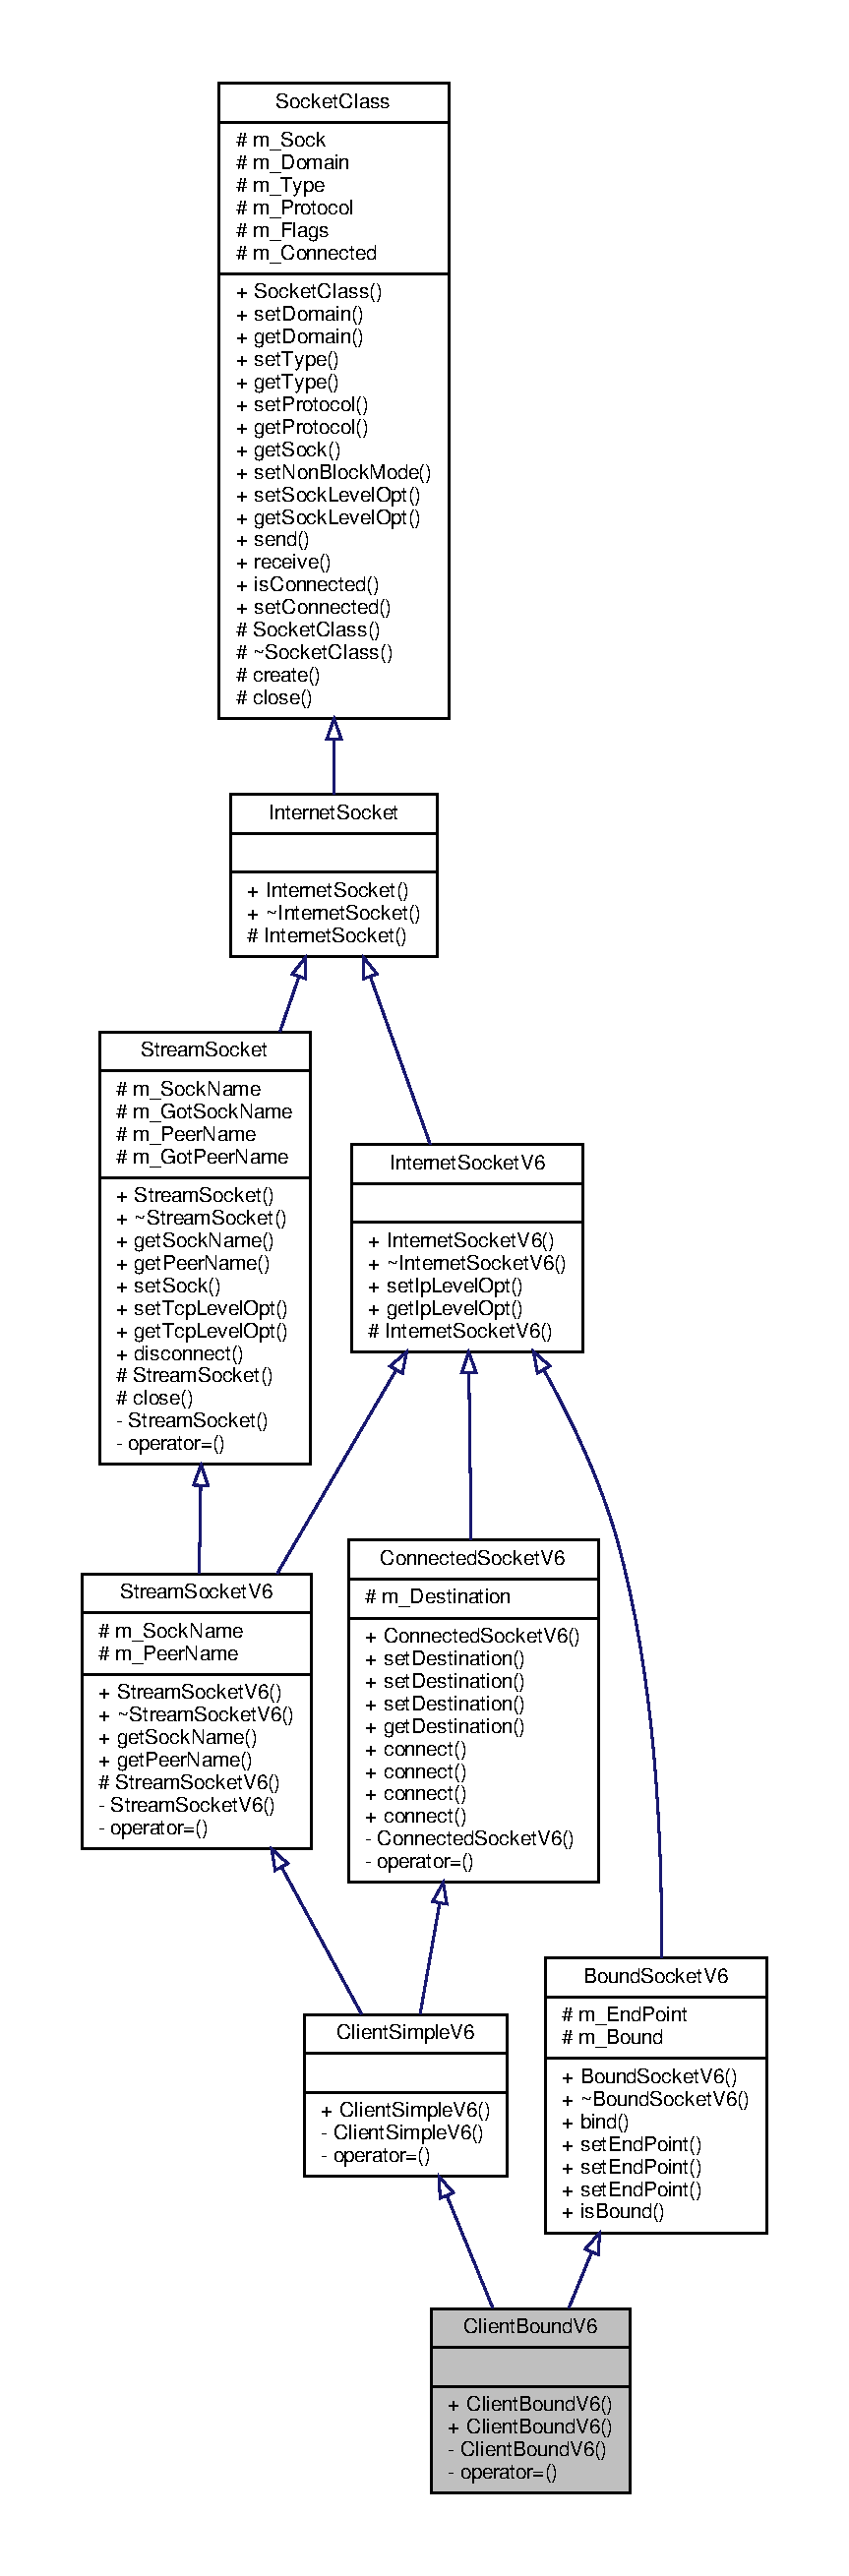
\includegraphics[height=550pt]{classClientBoundV6__inherit__graph}
\end{center}
\end{figure}
\subsection*{Public Member Functions}
\begin{DoxyCompactItemize}
\item 
\hyperlink{classClientBoundV6_a139f971557848afbc4201a16f081d441}{Client\+Bound\+V6} (short Port, in6\+\_\+addr Address=in6addr\+\_\+any, bool Late\+Bind=false)  throw (\+Sock\+Exception)
\item 
\hyperlink{classClientBoundV6_a41e5be655ddcf900ba3a166eed533982}{Client\+Bound\+V6} (short Port, const char $\ast$Address, bool Late\+Bind=false)  throw (\+Sock\+Exception)
\end{DoxyCompactItemize}
\subsection*{Private Member Functions}
\begin{DoxyCompactItemize}
\item 
\hyperlink{classClientBoundV6_a997dffff351c17df41e6cf2e8f69d1ee}{Client\+Bound\+V6} (\hyperlink{classClientBoundV6}{Client\+Bound\+V6} \&s)
\item 
\hyperlink{classClientBoundV6}{Client\+Bound\+V6} \& \hyperlink{classClientBoundV6_a0f04bf3652e27ac44ebc8e7694d7fcbe}{operator=} (\hyperlink{classClientBoundV6}{Client\+Bound\+V6} \&s)
\end{DoxyCompactItemize}
\subsection*{Additional Inherited Members}


\subsection{Detailed Description}
Client socket bound to specified port and address. 

\subsection{Constructor \& Destructor Documentation}
\mbox{\Hypertarget{classClientBoundV6_a139f971557848afbc4201a16f081d441}\label{classClientBoundV6_a139f971557848afbc4201a16f081d441}} 
\index{Client\+Bound\+V6@{Client\+Bound\+V6}!Client\+Bound\+V6@{Client\+Bound\+V6}}
\index{Client\+Bound\+V6@{Client\+Bound\+V6}!Client\+Bound\+V6@{Client\+Bound\+V6}}
\subsubsection{\texorpdfstring{Client\+Bound\+V6()}{ClientBoundV6()}\hspace{0.1cm}{\footnotesize\ttfamily [1/3]}}
{\footnotesize\ttfamily Client\+Bound\+V6\+::\+Client\+Bound\+V6 (\begin{DoxyParamCaption}\item[{short}]{Port,  }\item[{in6\+\_\+addr}]{Address = {\ttfamily in6addr\+\_\+any},  }\item[{bool}]{Late\+Bind = {\ttfamily false} }\end{DoxyParamCaption}) throw  \hyperlink{classSockException}{Sock\+Exception}) \hspace{0.3cm}{\ttfamily [inline]}}

Constructor. 
\begin{DoxyParams}{Parameters}
{\em Port} & \+: port number for bind in network byte order. \\
\hline
{\em Address} & \+: I\+Pv6 address for bind in network byte order. \\
\hline
{\em Late\+Bind} & \+: do bind now or later according to bind method call. \\
\hline
\end{DoxyParams}

\begin{DoxyExceptions}{Exceptions}
{\em Sock\+Exception.} & \\
\hline
\end{DoxyExceptions}
\mbox{\Hypertarget{classClientBoundV6_a41e5be655ddcf900ba3a166eed533982}\label{classClientBoundV6_a41e5be655ddcf900ba3a166eed533982}} 
\index{Client\+Bound\+V6@{Client\+Bound\+V6}!Client\+Bound\+V6@{Client\+Bound\+V6}}
\index{Client\+Bound\+V6@{Client\+Bound\+V6}!Client\+Bound\+V6@{Client\+Bound\+V6}}
\subsubsection{\texorpdfstring{Client\+Bound\+V6()}{ClientBoundV6()}\hspace{0.1cm}{\footnotesize\ttfamily [2/3]}}
{\footnotesize\ttfamily Client\+Bound\+V6\+::\+Client\+Bound\+V6 (\begin{DoxyParamCaption}\item[{short}]{Port,  }\item[{const char $\ast$}]{Address,  }\item[{bool}]{Late\+Bind = {\ttfamily false} }\end{DoxyParamCaption}) throw  \hyperlink{classSockException}{Sock\+Exception}) \hspace{0.3cm}{\ttfamily [inline]}}

Constructor. 
\begin{DoxyParams}{Parameters}
{\em Port} & \+: port number for bind in network byte order. \\
\hline
{\em Address} & \+: I\+Pv6 address for bind in textual notation. \\
\hline
{\em Late\+Bind} & \+: do bind now or later according to bind method call. \\
\hline
\end{DoxyParams}

\begin{DoxyExceptions}{Exceptions}
{\em Sock\+Exception.} & \\
\hline
\end{DoxyExceptions}
\mbox{\Hypertarget{classClientBoundV6_a997dffff351c17df41e6cf2e8f69d1ee}\label{classClientBoundV6_a997dffff351c17df41e6cf2e8f69d1ee}} 
\index{Client\+Bound\+V6@{Client\+Bound\+V6}!Client\+Bound\+V6@{Client\+Bound\+V6}}
\index{Client\+Bound\+V6@{Client\+Bound\+V6}!Client\+Bound\+V6@{Client\+Bound\+V6}}
\subsubsection{\texorpdfstring{Client\+Bound\+V6()}{ClientBoundV6()}\hspace{0.1cm}{\footnotesize\ttfamily [3/3]}}
{\footnotesize\ttfamily Client\+Bound\+V6\+::\+Client\+Bound\+V6 (\begin{DoxyParamCaption}\item[{\hyperlink{classClientBoundV6}{Client\+Bound\+V6} \&}]{s }\end{DoxyParamCaption})\hspace{0.3cm}{\ttfamily [private]}}

Copy constructor. Makes the class uncopyable. 

\subsection{Member Function Documentation}
\mbox{\Hypertarget{classClientBoundV6_a0f04bf3652e27ac44ebc8e7694d7fcbe}\label{classClientBoundV6_a0f04bf3652e27ac44ebc8e7694d7fcbe}} 
\index{Client\+Bound\+V6@{Client\+Bound\+V6}!operator=@{operator=}}
\index{operator=@{operator=}!Client\+Bound\+V6@{Client\+Bound\+V6}}
\subsubsection{\texorpdfstring{operator=()}{operator=()}}
{\footnotesize\ttfamily \hyperlink{classClientBoundV6}{Client\+Bound\+V6}\& Client\+Bound\+V6\+::operator= (\begin{DoxyParamCaption}\item[{\hyperlink{classClientBoundV6}{Client\+Bound\+V6} \&}]{s }\end{DoxyParamCaption})\hspace{0.3cm}{\ttfamily [private]}}

Operator assign. Makes the class uncopyable. 

The documentation for this class was generated from the following file\+:\begin{DoxyCompactItemize}
\item 
\hyperlink{ClientBoundV6_8h}{Client\+Bound\+V6.\+h}\end{DoxyCompactItemize}

\hypertarget{classClientSimple}{}\section{Client\+Simple Class Reference}
\label{classClientSimple}\index{Client\+Simple@{Client\+Simple}}


Stream oriented socket with connection ability.  




{\ttfamily \#include $<$Client\+Simple.\+h$>$}



Inheritance diagram for Client\+Simple\+:\nopagebreak
\begin{figure}[H]
\begin{center}
\leavevmode
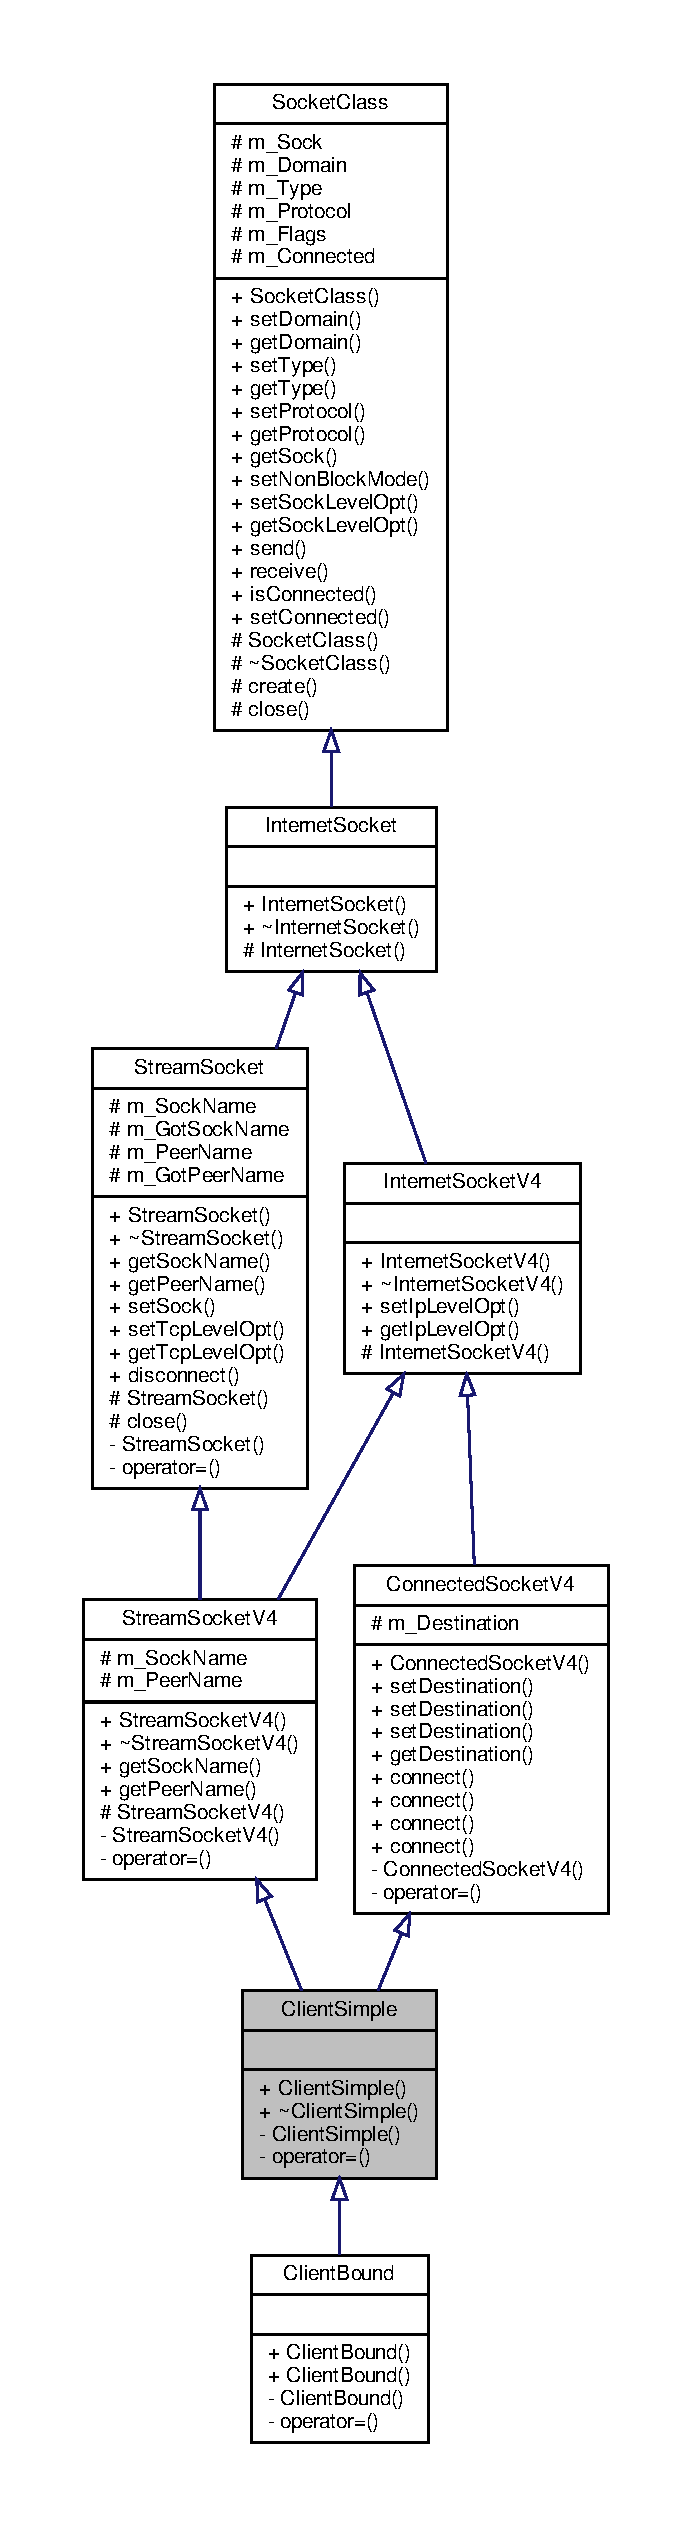
\includegraphics[height=550pt]{classClientSimple__inherit__graph}
\end{center}
\end{figure}
\subsection*{Public Member Functions}
\begin{DoxyCompactItemize}
\item 
\hyperlink{classClientSimple_a29949bd6c34b124b0ced310e9b400664}{Client\+Simple} ()
\item 
virtual \hyperlink{classClientSimple_ae095fffdeca191749c72be5502b7b64b}{$\sim$\+Client\+Simple} ()
\end{DoxyCompactItemize}
\subsection*{Private Member Functions}
\begin{DoxyCompactItemize}
\item 
\hyperlink{classClientSimple_a5ef01407050f965155efe56ad1338ad3}{Client\+Simple} (\hyperlink{classClientSimple}{Client\+Simple} \&s)
\item 
\hyperlink{classClientSimple}{Client\+Simple} \& \hyperlink{classClientSimple_a59b6462085e8ac3aa1b634f28fe7efb4}{operator=} (\hyperlink{classClientSimple}{Client\+Simple} \&s)
\end{DoxyCompactItemize}
\subsection*{Additional Inherited Members}


\subsection{Detailed Description}
Stream oriented socket with connection ability. 

\subsection{Constructor \& Destructor Documentation}
\mbox{\Hypertarget{classClientSimple_a29949bd6c34b124b0ced310e9b400664}\label{classClientSimple_a29949bd6c34b124b0ced310e9b400664}} 
\index{Client\+Simple@{Client\+Simple}!Client\+Simple@{Client\+Simple}}
\index{Client\+Simple@{Client\+Simple}!Client\+Simple@{Client\+Simple}}
\subsubsection{\texorpdfstring{Client\+Simple()}{ClientSimple()}\hspace{0.1cm}{\footnotesize\ttfamily [1/2]}}
{\footnotesize\ttfamily Client\+Simple\+::\+Client\+Simple (\begin{DoxyParamCaption}{ }\end{DoxyParamCaption})\hspace{0.3cm}{\ttfamily [inline]}}

Constructor. Default constructor. \mbox{\Hypertarget{classClientSimple_ae095fffdeca191749c72be5502b7b64b}\label{classClientSimple_ae095fffdeca191749c72be5502b7b64b}} 
\index{Client\+Simple@{Client\+Simple}!````~Client\+Simple@{$\sim$\+Client\+Simple}}
\index{````~Client\+Simple@{$\sim$\+Client\+Simple}!Client\+Simple@{Client\+Simple}}
\subsubsection{\texorpdfstring{$\sim$\+Client\+Simple()}{~ClientSimple()}}
{\footnotesize\ttfamily virtual Client\+Simple\+::$\sim$\+Client\+Simple (\begin{DoxyParamCaption}{ }\end{DoxyParamCaption})\hspace{0.3cm}{\ttfamily [inline]}, {\ttfamily [virtual]}}

\mbox{\Hypertarget{classClientSimple_a5ef01407050f965155efe56ad1338ad3}\label{classClientSimple_a5ef01407050f965155efe56ad1338ad3}} 
\index{Client\+Simple@{Client\+Simple}!Client\+Simple@{Client\+Simple}}
\index{Client\+Simple@{Client\+Simple}!Client\+Simple@{Client\+Simple}}
\subsubsection{\texorpdfstring{Client\+Simple()}{ClientSimple()}\hspace{0.1cm}{\footnotesize\ttfamily [2/2]}}
{\footnotesize\ttfamily Client\+Simple\+::\+Client\+Simple (\begin{DoxyParamCaption}\item[{\hyperlink{classClientSimple}{Client\+Simple} \&}]{s }\end{DoxyParamCaption})\hspace{0.3cm}{\ttfamily [private]}}

Copy constructor. Makes the class uncopyable. 

\subsection{Member Function Documentation}
\mbox{\Hypertarget{classClientSimple_a59b6462085e8ac3aa1b634f28fe7efb4}\label{classClientSimple_a59b6462085e8ac3aa1b634f28fe7efb4}} 
\index{Client\+Simple@{Client\+Simple}!operator=@{operator=}}
\index{operator=@{operator=}!Client\+Simple@{Client\+Simple}}
\subsubsection{\texorpdfstring{operator=()}{operator=()}}
{\footnotesize\ttfamily \hyperlink{classClientSimple}{Client\+Simple}\& Client\+Simple\+::operator= (\begin{DoxyParamCaption}\item[{\hyperlink{classClientSimple}{Client\+Simple} \&}]{s }\end{DoxyParamCaption})\hspace{0.3cm}{\ttfamily [private]}}

Operator assign. Makes the class uncopyable. 

The documentation for this class was generated from the following file\+:\begin{DoxyCompactItemize}
\item 
\hyperlink{ClientSimple_8h}{Client\+Simple.\+h}\end{DoxyCompactItemize}

\hypertarget{classClientSimpleV6}{}\section{Client\+Simple\+V6 Class Reference}
\label{classClientSimpleV6}\index{Client\+Simple\+V6@{Client\+Simple\+V6}}


Stream oriented socket with connection ability for I\+Pv6.  




{\ttfamily \#include $<$Client\+Simple\+V6.\+h$>$}



Inheritance diagram for Client\+Simple\+V6\+:\nopagebreak
\begin{figure}[H]
\begin{center}
\leavevmode
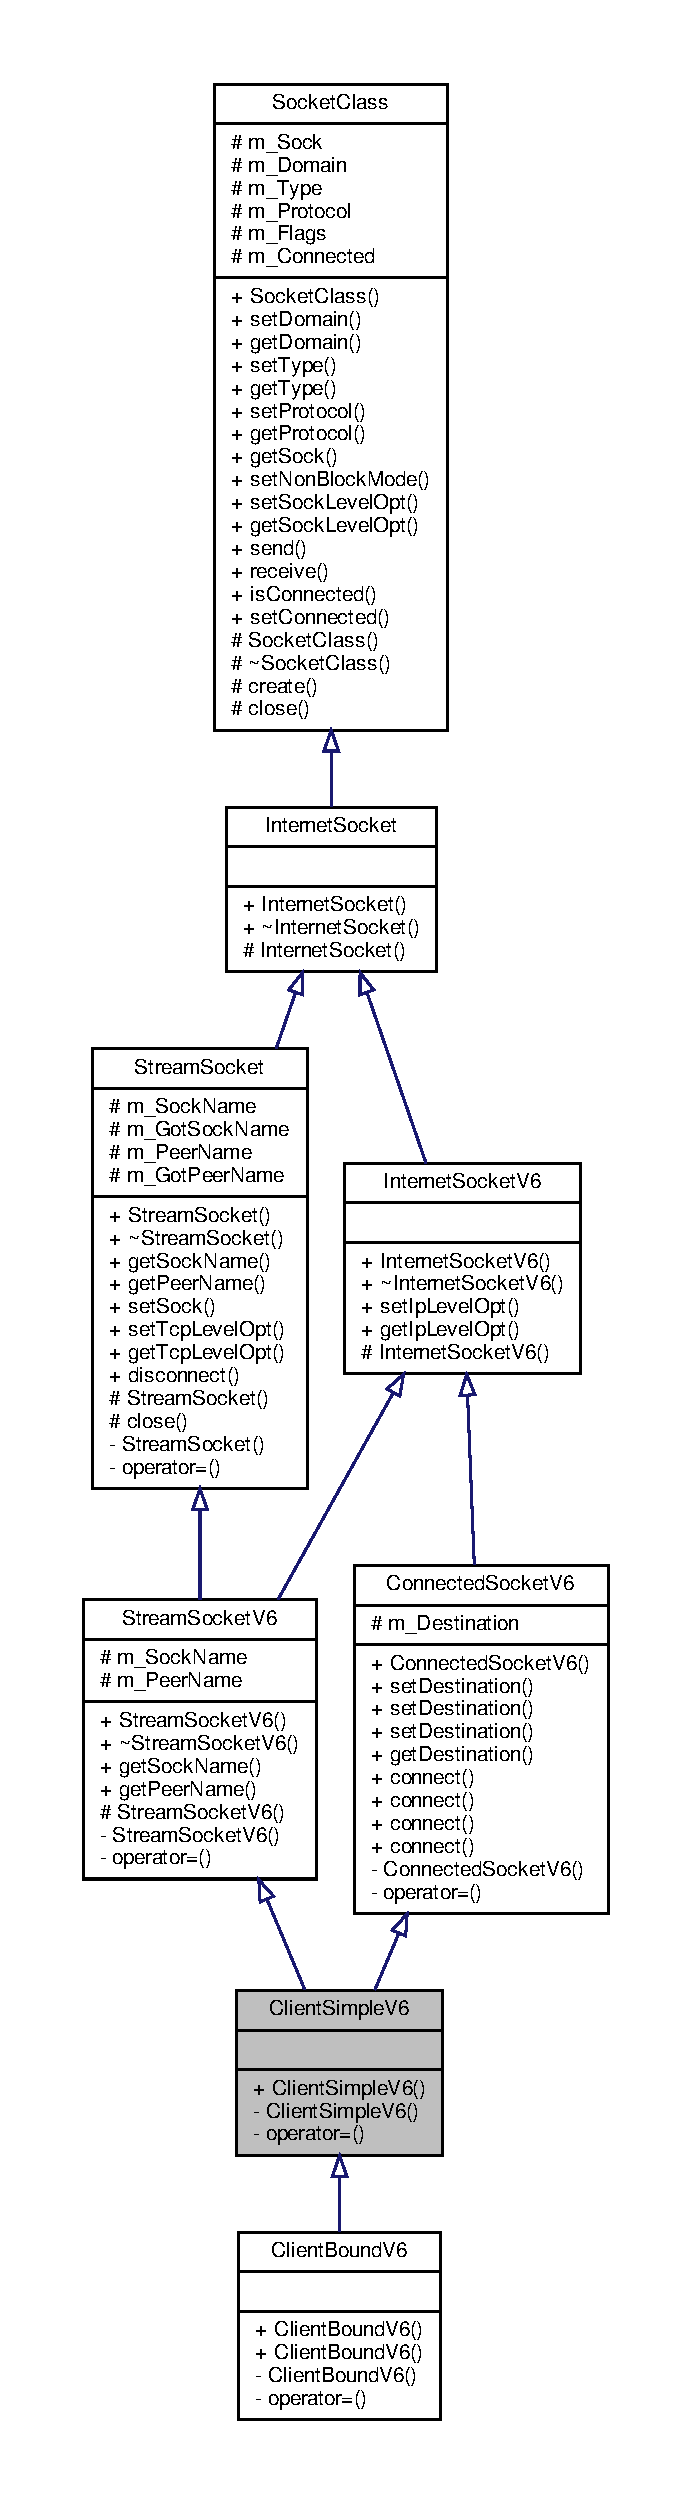
\includegraphics[height=550pt]{classClientSimpleV6__inherit__graph}
\end{center}
\end{figure}
\subsection*{Public Member Functions}
\begin{DoxyCompactItemize}
\item 
\hyperlink{classClientSimpleV6_a9e064f9b3c0b4b33f92b14c4eb8f5ac4}{Client\+Simple\+V6} ()
\end{DoxyCompactItemize}
\subsection*{Private Member Functions}
\begin{DoxyCompactItemize}
\item 
\hyperlink{classClientSimpleV6_a11b2623f14326d304d9679f04499bea2}{Client\+Simple\+V6} (\hyperlink{classClientSimpleV6}{Client\+Simple\+V6} \&s)
\item 
\hyperlink{classClientSimpleV6}{Client\+Simple\+V6} \& \hyperlink{classClientSimpleV6_a9ca646eeda4e4d5670c0eb70b915d3e4}{operator=} (\hyperlink{classClientSimpleV6}{Client\+Simple\+V6} \&s)
\end{DoxyCompactItemize}
\subsection*{Additional Inherited Members}


\subsection{Detailed Description}
Stream oriented socket with connection ability for I\+Pv6. 

\subsection{Constructor \& Destructor Documentation}
\mbox{\Hypertarget{classClientSimpleV6_a9e064f9b3c0b4b33f92b14c4eb8f5ac4}\label{classClientSimpleV6_a9e064f9b3c0b4b33f92b14c4eb8f5ac4}} 
\index{Client\+Simple\+V6@{Client\+Simple\+V6}!Client\+Simple\+V6@{Client\+Simple\+V6}}
\index{Client\+Simple\+V6@{Client\+Simple\+V6}!Client\+Simple\+V6@{Client\+Simple\+V6}}
\subsubsection{\texorpdfstring{Client\+Simple\+V6()}{ClientSimpleV6()}\hspace{0.1cm}{\footnotesize\ttfamily [1/2]}}
{\footnotesize\ttfamily Client\+Simple\+V6\+::\+Client\+Simple\+V6 (\begin{DoxyParamCaption}{ }\end{DoxyParamCaption})\hspace{0.3cm}{\ttfamily [inline]}}

Constructor. Default constructor. \mbox{\Hypertarget{classClientSimpleV6_a11b2623f14326d304d9679f04499bea2}\label{classClientSimpleV6_a11b2623f14326d304d9679f04499bea2}} 
\index{Client\+Simple\+V6@{Client\+Simple\+V6}!Client\+Simple\+V6@{Client\+Simple\+V6}}
\index{Client\+Simple\+V6@{Client\+Simple\+V6}!Client\+Simple\+V6@{Client\+Simple\+V6}}
\subsubsection{\texorpdfstring{Client\+Simple\+V6()}{ClientSimpleV6()}\hspace{0.1cm}{\footnotesize\ttfamily [2/2]}}
{\footnotesize\ttfamily Client\+Simple\+V6\+::\+Client\+Simple\+V6 (\begin{DoxyParamCaption}\item[{\hyperlink{classClientSimpleV6}{Client\+Simple\+V6} \&}]{s }\end{DoxyParamCaption})\hspace{0.3cm}{\ttfamily [private]}}

Copy constructor. Makes the class uncopyable. 

\subsection{Member Function Documentation}
\mbox{\Hypertarget{classClientSimpleV6_a9ca646eeda4e4d5670c0eb70b915d3e4}\label{classClientSimpleV6_a9ca646eeda4e4d5670c0eb70b915d3e4}} 
\index{Client\+Simple\+V6@{Client\+Simple\+V6}!operator=@{operator=}}
\index{operator=@{operator=}!Client\+Simple\+V6@{Client\+Simple\+V6}}
\subsubsection{\texorpdfstring{operator=()}{operator=()}}
{\footnotesize\ttfamily \hyperlink{classClientSimpleV6}{Client\+Simple\+V6}\& Client\+Simple\+V6\+::operator= (\begin{DoxyParamCaption}\item[{\hyperlink{classClientSimpleV6}{Client\+Simple\+V6} \&}]{s }\end{DoxyParamCaption})\hspace{0.3cm}{\ttfamily [private]}}

Operator assign. Makes the class uncopyable. 

The documentation for this class was generated from the following file\+:\begin{DoxyCompactItemize}
\item 
\hyperlink{ClientSimpleV6_8h}{Client\+Simple\+V6.\+h}\end{DoxyCompactItemize}

\hypertarget{classConnectedSocketV4}{}\section{Connected\+Socket\+V4 Class Reference}
\label{classConnectedSocketV4}\index{Connected\+Socket\+V4@{Connected\+Socket\+V4}}


Socket that can connect to another.  




{\ttfamily \#include $<$Connected\+Socket\+V4.\+h$>$}



Inheritance diagram for Connected\+Socket\+V4\+:\nopagebreak
\begin{figure}[H]
\begin{center}
\leavevmode
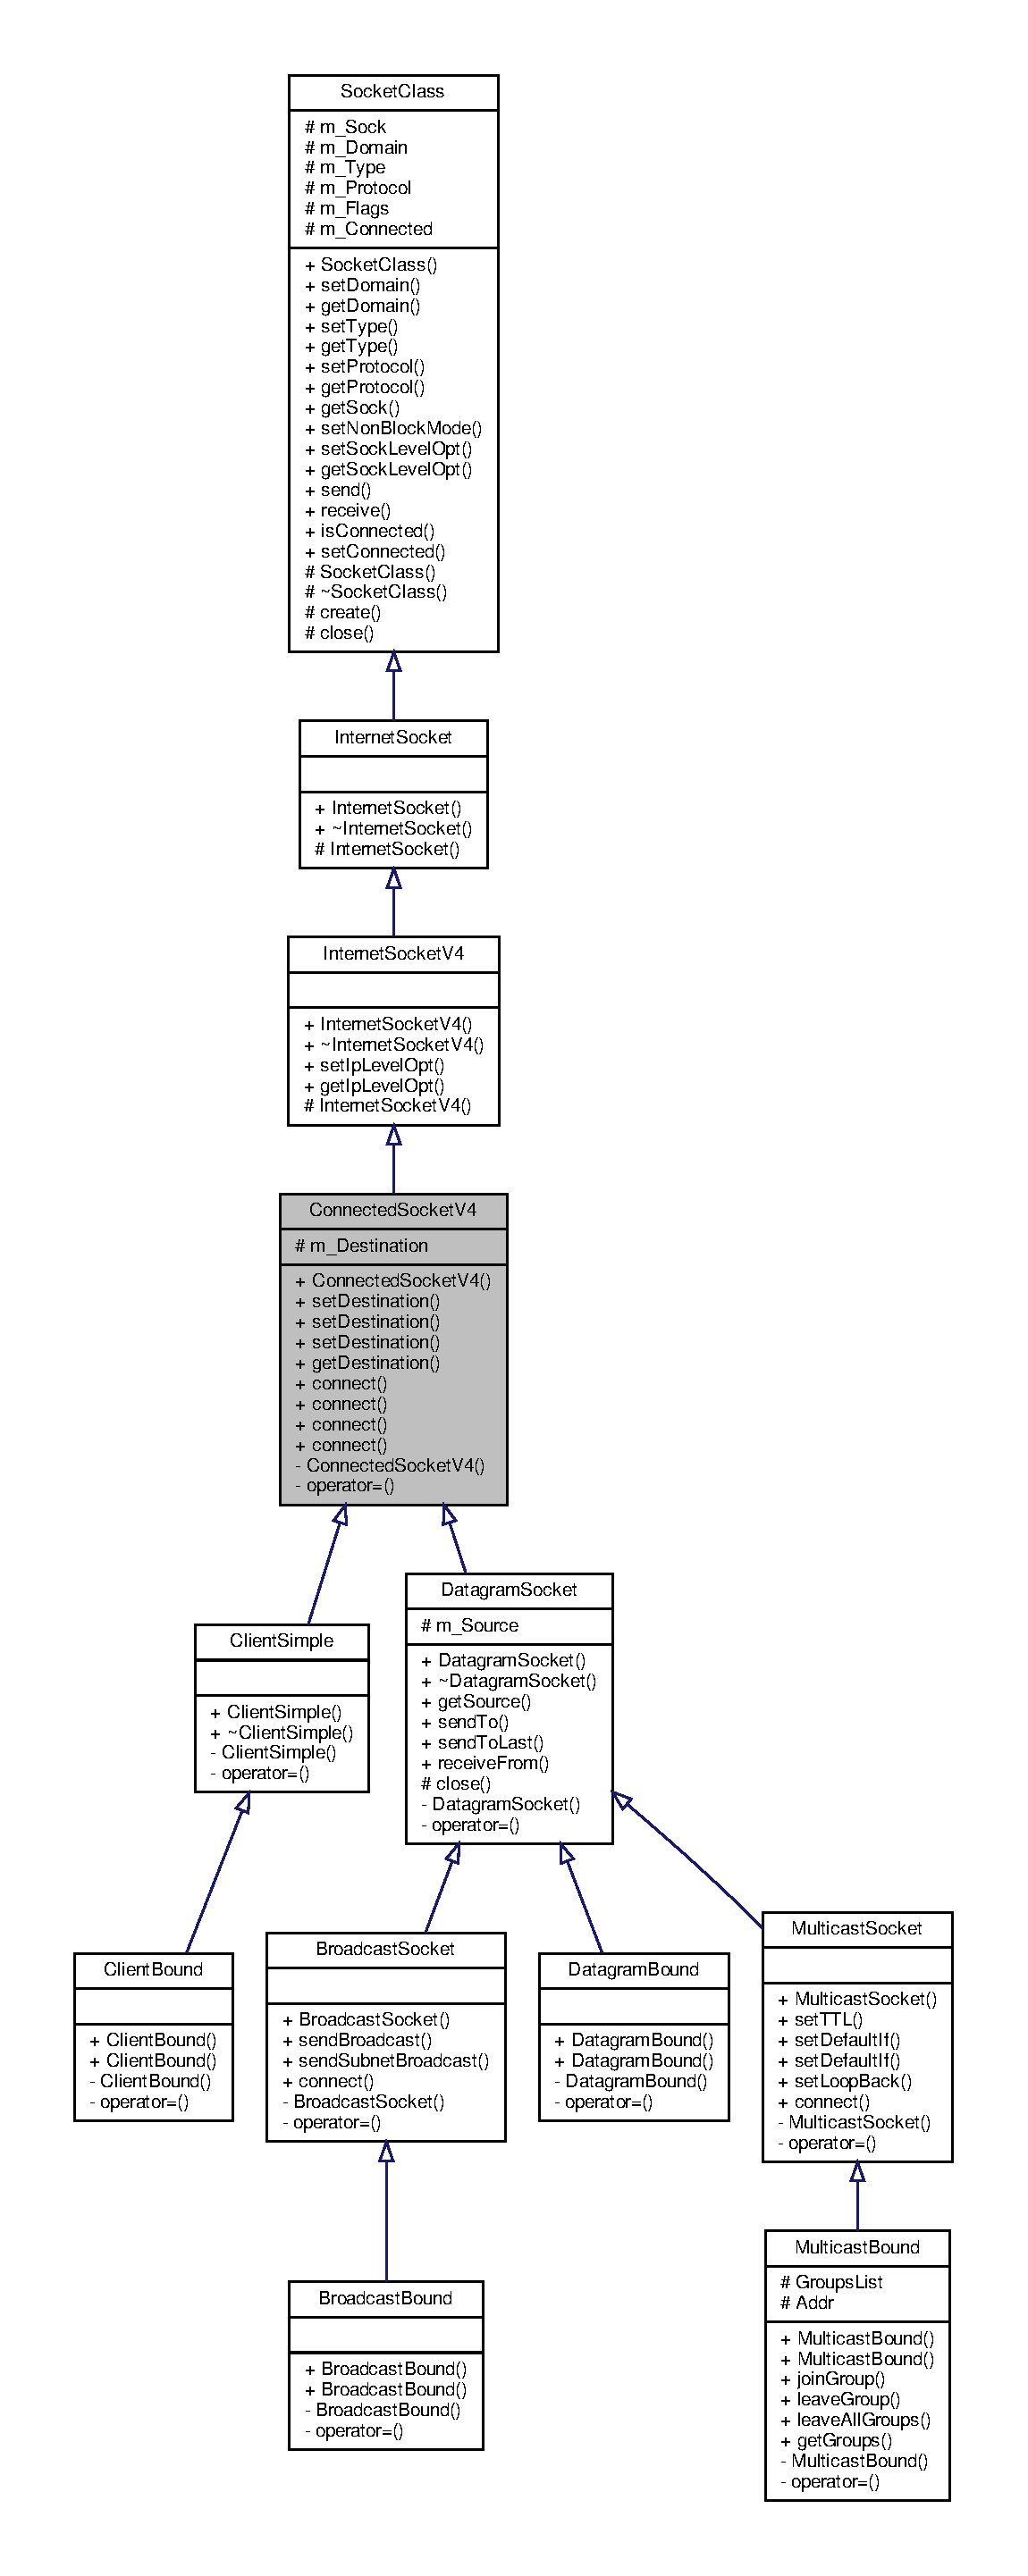
\includegraphics[height=550pt]{classConnectedSocketV4__inherit__graph}
\end{center}
\end{figure}
\subsection*{Public Member Functions}
\begin{DoxyCompactItemize}
\item 
\hyperlink{classConnectedSocketV4_ab6fd7088764d07f276a6be26e2dd8334}{Connected\+Socket\+V4} ()
\item 
void \hyperlink{classConnectedSocketV4_a550cc6530361565ea80e0b2ce892402e}{set\+Destination} (sockaddr\+\_\+in Dest)
\item 
void \hyperlink{classConnectedSocketV4_a8f069939a6796530ba9f2a781e787db7}{set\+Destination} (in\+\_\+addr\+\_\+t Address, short Port)
\item 
void \hyperlink{classConnectedSocketV4_a9ba0783ad8bdeabd25a1ba5a2a1178fc}{set\+Destination} (const char $\ast$Address, short Port)
\item 
sockaddr\+\_\+in \& \hyperlink{classConnectedSocketV4_aba8df9ab0af83ab20a522e32b6d8e3bb}{get\+Destination} ()
\item 
virtual void \hyperlink{classConnectedSocketV4_a034d0c949fa1a0f14c136f839915d1a4}{connect} ()
\item 
void \hyperlink{classConnectedSocketV4_a9998be702c3a10a686bc6dfd914a10fe}{connect} (in\+\_\+addr\+\_\+t Address, short Port)
\item 
void \hyperlink{classConnectedSocketV4_af094a90dbff1746f213f7dcb2a46a0b7}{connect} (const char $\ast$Address, short Port)
\item 
void \hyperlink{classConnectedSocketV4_a751123cd0d6a737e87748ce2a175cd47}{connect} (sockaddr\+\_\+in Dest)
\end{DoxyCompactItemize}
\subsection*{Protected Attributes}
\begin{DoxyCompactItemize}
\item 
sockaddr\+\_\+in \hyperlink{classConnectedSocketV4_ab07c2124a1a10a7f402bba27e457d15d}{m\+\_\+\+Destination}
\begin{DoxyCompactList}\small\item\em Destination endpoint properties. \end{DoxyCompactList}\end{DoxyCompactItemize}
\subsection*{Private Member Functions}
\begin{DoxyCompactItemize}
\item 
\hyperlink{classConnectedSocketV4_a12724341a7a57fd8b5d79bce7b1dd385}{Connected\+Socket\+V4} (\hyperlink{classConnectedSocketV4}{Connected\+Socket\+V4} \&s)
\item 
\hyperlink{classConnectedSocketV4}{Connected\+Socket\+V4} \& \hyperlink{classConnectedSocketV4_a9fcb520d8f3aa2454155b6a6b5e97b39}{operator=} (\hyperlink{classConnectedSocketV4}{Connected\+Socket\+V4} \&s)
\end{DoxyCompactItemize}
\subsection*{Additional Inherited Members}


\subsection{Detailed Description}
Socket that can connect to another. 

\subsection{Constructor \& Destructor Documentation}
\mbox{\Hypertarget{classConnectedSocketV4_ab6fd7088764d07f276a6be26e2dd8334}\label{classConnectedSocketV4_ab6fd7088764d07f276a6be26e2dd8334}} 
\index{Connected\+Socket\+V4@{Connected\+Socket\+V4}!Connected\+Socket\+V4@{Connected\+Socket\+V4}}
\index{Connected\+Socket\+V4@{Connected\+Socket\+V4}!Connected\+Socket\+V4@{Connected\+Socket\+V4}}
\subsubsection{\texorpdfstring{Connected\+Socket\+V4()}{ConnectedSocketV4()}\hspace{0.1cm}{\footnotesize\ttfamily [1/2]}}
{\footnotesize\ttfamily Connected\+Socket\+V4\+::\+Connected\+Socket\+V4 (\begin{DoxyParamCaption}{ }\end{DoxyParamCaption})\hspace{0.3cm}{\ttfamily [inline]}}

Constructor. Default constructor. \mbox{\Hypertarget{classConnectedSocketV4_a12724341a7a57fd8b5d79bce7b1dd385}\label{classConnectedSocketV4_a12724341a7a57fd8b5d79bce7b1dd385}} 
\index{Connected\+Socket\+V4@{Connected\+Socket\+V4}!Connected\+Socket\+V4@{Connected\+Socket\+V4}}
\index{Connected\+Socket\+V4@{Connected\+Socket\+V4}!Connected\+Socket\+V4@{Connected\+Socket\+V4}}
\subsubsection{\texorpdfstring{Connected\+Socket\+V4()}{ConnectedSocketV4()}\hspace{0.1cm}{\footnotesize\ttfamily [2/2]}}
{\footnotesize\ttfamily Connected\+Socket\+V4\+::\+Connected\+Socket\+V4 (\begin{DoxyParamCaption}\item[{\hyperlink{classConnectedSocketV4}{Connected\+Socket\+V4} \&}]{s }\end{DoxyParamCaption})\hspace{0.3cm}{\ttfamily [private]}}

Copy constructor. Makes the class uncopyable . 

\subsection{Member Function Documentation}
\mbox{\Hypertarget{classConnectedSocketV4_a034d0c949fa1a0f14c136f839915d1a4}\label{classConnectedSocketV4_a034d0c949fa1a0f14c136f839915d1a4}} 
\index{Connected\+Socket\+V4@{Connected\+Socket\+V4}!connect@{connect}}
\index{connect@{connect}!Connected\+Socket\+V4@{Connected\+Socket\+V4}}
\subsubsection{\texorpdfstring{connect()}{connect()}\hspace{0.1cm}{\footnotesize\ttfamily [1/4]}}
{\footnotesize\ttfamily void Connected\+Socket\+V4\+::connect (\begin{DoxyParamCaption}{ }\end{DoxyParamCaption})\hspace{0.3cm}{\ttfamily [virtual]}}

Connect to destination endpoint. 
\begin{DoxyExceptions}{Exceptions}
{\em Sock\+Exception.} & \\
\hline
\end{DoxyExceptions}


Reimplemented in \hyperlink{classBroadcastSocket_a330f3448f2c53eef77af683cfd94eafd}{Broadcast\+Socket}, and \hyperlink{classMulticastSocket_a30ffd3d7fe782c2d74d69d994e465a4d}{Multicast\+Socket}.

\mbox{\Hypertarget{classConnectedSocketV4_a9998be702c3a10a686bc6dfd914a10fe}\label{classConnectedSocketV4_a9998be702c3a10a686bc6dfd914a10fe}} 
\index{Connected\+Socket\+V4@{Connected\+Socket\+V4}!connect@{connect}}
\index{connect@{connect}!Connected\+Socket\+V4@{Connected\+Socket\+V4}}
\subsubsection{\texorpdfstring{connect()}{connect()}\hspace{0.1cm}{\footnotesize\ttfamily [2/4]}}
{\footnotesize\ttfamily void Connected\+Socket\+V4\+::connect (\begin{DoxyParamCaption}\item[{in\+\_\+addr\+\_\+t}]{Address,  }\item[{short}]{Port }\end{DoxyParamCaption})\hspace{0.3cm}{\ttfamily [inline]}}

Connect to destination endpoint. 
\begin{DoxyParams}{Parameters}
{\em Address} & \+: I\+Pv4 address in network byte order. \\
\hline
{\em Port} & \+: port number in network byte order. \\
\hline
\end{DoxyParams}

\begin{DoxyExceptions}{Exceptions}
{\em Sock\+Exception.} & \\
\hline
\end{DoxyExceptions}
\mbox{\Hypertarget{classConnectedSocketV4_af094a90dbff1746f213f7dcb2a46a0b7}\label{classConnectedSocketV4_af094a90dbff1746f213f7dcb2a46a0b7}} 
\index{Connected\+Socket\+V4@{Connected\+Socket\+V4}!connect@{connect}}
\index{connect@{connect}!Connected\+Socket\+V4@{Connected\+Socket\+V4}}
\subsubsection{\texorpdfstring{connect()}{connect()}\hspace{0.1cm}{\footnotesize\ttfamily [3/4]}}
{\footnotesize\ttfamily void Connected\+Socket\+V4\+::connect (\begin{DoxyParamCaption}\item[{const char $\ast$}]{Address,  }\item[{short}]{Port }\end{DoxyParamCaption})\hspace{0.3cm}{\ttfamily [inline]}}

Connect to destination endpoint. 
\begin{DoxyParams}{Parameters}
{\em Address} & \+: I\+Pv4 address in decimal dot notation. \\
\hline
{\em Port} & \+: port number in network byte order. \\
\hline
\end{DoxyParams}

\begin{DoxyExceptions}{Exceptions}
{\em Sock\+Exception.} & \\
\hline
\end{DoxyExceptions}
\mbox{\Hypertarget{classConnectedSocketV4_a751123cd0d6a737e87748ce2a175cd47}\label{classConnectedSocketV4_a751123cd0d6a737e87748ce2a175cd47}} 
\index{Connected\+Socket\+V4@{Connected\+Socket\+V4}!connect@{connect}}
\index{connect@{connect}!Connected\+Socket\+V4@{Connected\+Socket\+V4}}
\subsubsection{\texorpdfstring{connect()}{connect()}\hspace{0.1cm}{\footnotesize\ttfamily [4/4]}}
{\footnotesize\ttfamily void Connected\+Socket\+V4\+::connect (\begin{DoxyParamCaption}\item[{sockaddr\+\_\+in}]{Dest }\end{DoxyParamCaption})\hspace{0.3cm}{\ttfamily [inline]}}

Connect to destination endpoint. 
\begin{DoxyParams}{Parameters}
{\em Dest} & \+: sockaddr\+\_\+in structure filled with destination endpoint properties. \\
\hline
\end{DoxyParams}

\begin{DoxyExceptions}{Exceptions}
{\em Sock\+Exception.} & \\
\hline
\end{DoxyExceptions}
\mbox{\Hypertarget{classConnectedSocketV4_aba8df9ab0af83ab20a522e32b6d8e3bb}\label{classConnectedSocketV4_aba8df9ab0af83ab20a522e32b6d8e3bb}} 
\index{Connected\+Socket\+V4@{Connected\+Socket\+V4}!get\+Destination@{get\+Destination}}
\index{get\+Destination@{get\+Destination}!Connected\+Socket\+V4@{Connected\+Socket\+V4}}
\subsubsection{\texorpdfstring{get\+Destination()}{getDestination()}}
{\footnotesize\ttfamily sockaddr\+\_\+in\& Connected\+Socket\+V4\+::get\+Destination (\begin{DoxyParamCaption}{ }\end{DoxyParamCaption})\hspace{0.3cm}{\ttfamily [inline]}}

Deliver destination endpoint properties. \begin{DoxyReturn}{Returns}
sockaddr\+\_\+in structure filled with endpoint properties. 
\end{DoxyReturn}
\mbox{\Hypertarget{classConnectedSocketV4_a9fcb520d8f3aa2454155b6a6b5e97b39}\label{classConnectedSocketV4_a9fcb520d8f3aa2454155b6a6b5e97b39}} 
\index{Connected\+Socket\+V4@{Connected\+Socket\+V4}!operator=@{operator=}}
\index{operator=@{operator=}!Connected\+Socket\+V4@{Connected\+Socket\+V4}}
\subsubsection{\texorpdfstring{operator=()}{operator=()}}
{\footnotesize\ttfamily \hyperlink{classConnectedSocketV4}{Connected\+Socket\+V4}\& Connected\+Socket\+V4\+::operator= (\begin{DoxyParamCaption}\item[{\hyperlink{classConnectedSocketV4}{Connected\+Socket\+V4} \&}]{s }\end{DoxyParamCaption})\hspace{0.3cm}{\ttfamily [private]}}

Operator assign. Makes the class uncopyable . \mbox{\Hypertarget{classConnectedSocketV4_a550cc6530361565ea80e0b2ce892402e}\label{classConnectedSocketV4_a550cc6530361565ea80e0b2ce892402e}} 
\index{Connected\+Socket\+V4@{Connected\+Socket\+V4}!set\+Destination@{set\+Destination}}
\index{set\+Destination@{set\+Destination}!Connected\+Socket\+V4@{Connected\+Socket\+V4}}
\subsubsection{\texorpdfstring{set\+Destination()}{setDestination()}\hspace{0.1cm}{\footnotesize\ttfamily [1/3]}}
{\footnotesize\ttfamily void Connected\+Socket\+V4\+::set\+Destination (\begin{DoxyParamCaption}\item[{sockaddr\+\_\+in}]{Dest }\end{DoxyParamCaption})\hspace{0.3cm}{\ttfamily [inline]}}

Set connection destination endpoint. 
\begin{DoxyParams}{Parameters}
{\em Dest} & \+: sockaddr\+\_\+in structure filled with destination endpoint properties. \\
\hline
\end{DoxyParams}
\mbox{\Hypertarget{classConnectedSocketV4_a8f069939a6796530ba9f2a781e787db7}\label{classConnectedSocketV4_a8f069939a6796530ba9f2a781e787db7}} 
\index{Connected\+Socket\+V4@{Connected\+Socket\+V4}!set\+Destination@{set\+Destination}}
\index{set\+Destination@{set\+Destination}!Connected\+Socket\+V4@{Connected\+Socket\+V4}}
\subsubsection{\texorpdfstring{set\+Destination()}{setDestination()}\hspace{0.1cm}{\footnotesize\ttfamily [2/3]}}
{\footnotesize\ttfamily void Connected\+Socket\+V4\+::set\+Destination (\begin{DoxyParamCaption}\item[{in\+\_\+addr\+\_\+t}]{Address,  }\item[{short}]{Port }\end{DoxyParamCaption})}

Set connection destination endpoint. 
\begin{DoxyParams}{Parameters}
{\em Address} & \+: I\+Pv4 address in network byte order. \\
\hline
{\em Port} & \+: port number in network byte order. \\
\hline
\end{DoxyParams}
\mbox{\Hypertarget{classConnectedSocketV4_a9ba0783ad8bdeabd25a1ba5a2a1178fc}\label{classConnectedSocketV4_a9ba0783ad8bdeabd25a1ba5a2a1178fc}} 
\index{Connected\+Socket\+V4@{Connected\+Socket\+V4}!set\+Destination@{set\+Destination}}
\index{set\+Destination@{set\+Destination}!Connected\+Socket\+V4@{Connected\+Socket\+V4}}
\subsubsection{\texorpdfstring{set\+Destination()}{setDestination()}\hspace{0.1cm}{\footnotesize\ttfamily [3/3]}}
{\footnotesize\ttfamily void Connected\+Socket\+V4\+::set\+Destination (\begin{DoxyParamCaption}\item[{const char $\ast$}]{Address,  }\item[{short}]{Port }\end{DoxyParamCaption})}

Set connection destination endpoint. 
\begin{DoxyParams}{Parameters}
{\em Address} & \+: I\+Pv4 address in decimal dot notation. \\
\hline
{\em Port} & \+: port number in network byte order. \\
\hline
\end{DoxyParams}


\subsection{Member Data Documentation}
\mbox{\Hypertarget{classConnectedSocketV4_ab07c2124a1a10a7f402bba27e457d15d}\label{classConnectedSocketV4_ab07c2124a1a10a7f402bba27e457d15d}} 
\index{Connected\+Socket\+V4@{Connected\+Socket\+V4}!m\+\_\+\+Destination@{m\+\_\+\+Destination}}
\index{m\+\_\+\+Destination@{m\+\_\+\+Destination}!Connected\+Socket\+V4@{Connected\+Socket\+V4}}
\subsubsection{\texorpdfstring{m\+\_\+\+Destination}{m\_Destination}}
{\footnotesize\ttfamily sockaddr\+\_\+in Connected\+Socket\+V4\+::m\+\_\+\+Destination\hspace{0.3cm}{\ttfamily [protected]}}



Destination endpoint properties. 



The documentation for this class was generated from the following files\+:\begin{DoxyCompactItemize}
\item 
\hyperlink{ConnectedSocketV4_8h}{Connected\+Socket\+V4.\+h}\item 
\hyperlink{ConnectedSocketV4_8cpp}{Connected\+Socket\+V4.\+cpp}\end{DoxyCompactItemize}

\hypertarget{classConnectedSocketV6}{}\section{Connected\+Socket\+V6 Class Reference}
\label{classConnectedSocketV6}\index{Connected\+Socket\+V6@{Connected\+Socket\+V6}}


Socket that can connect to another.  




{\ttfamily \#include $<$Connected\+Socket\+V6.\+h$>$}



Inheritance diagram for Connected\+Socket\+V6\+:\nopagebreak
\begin{figure}[H]
\begin{center}
\leavevmode
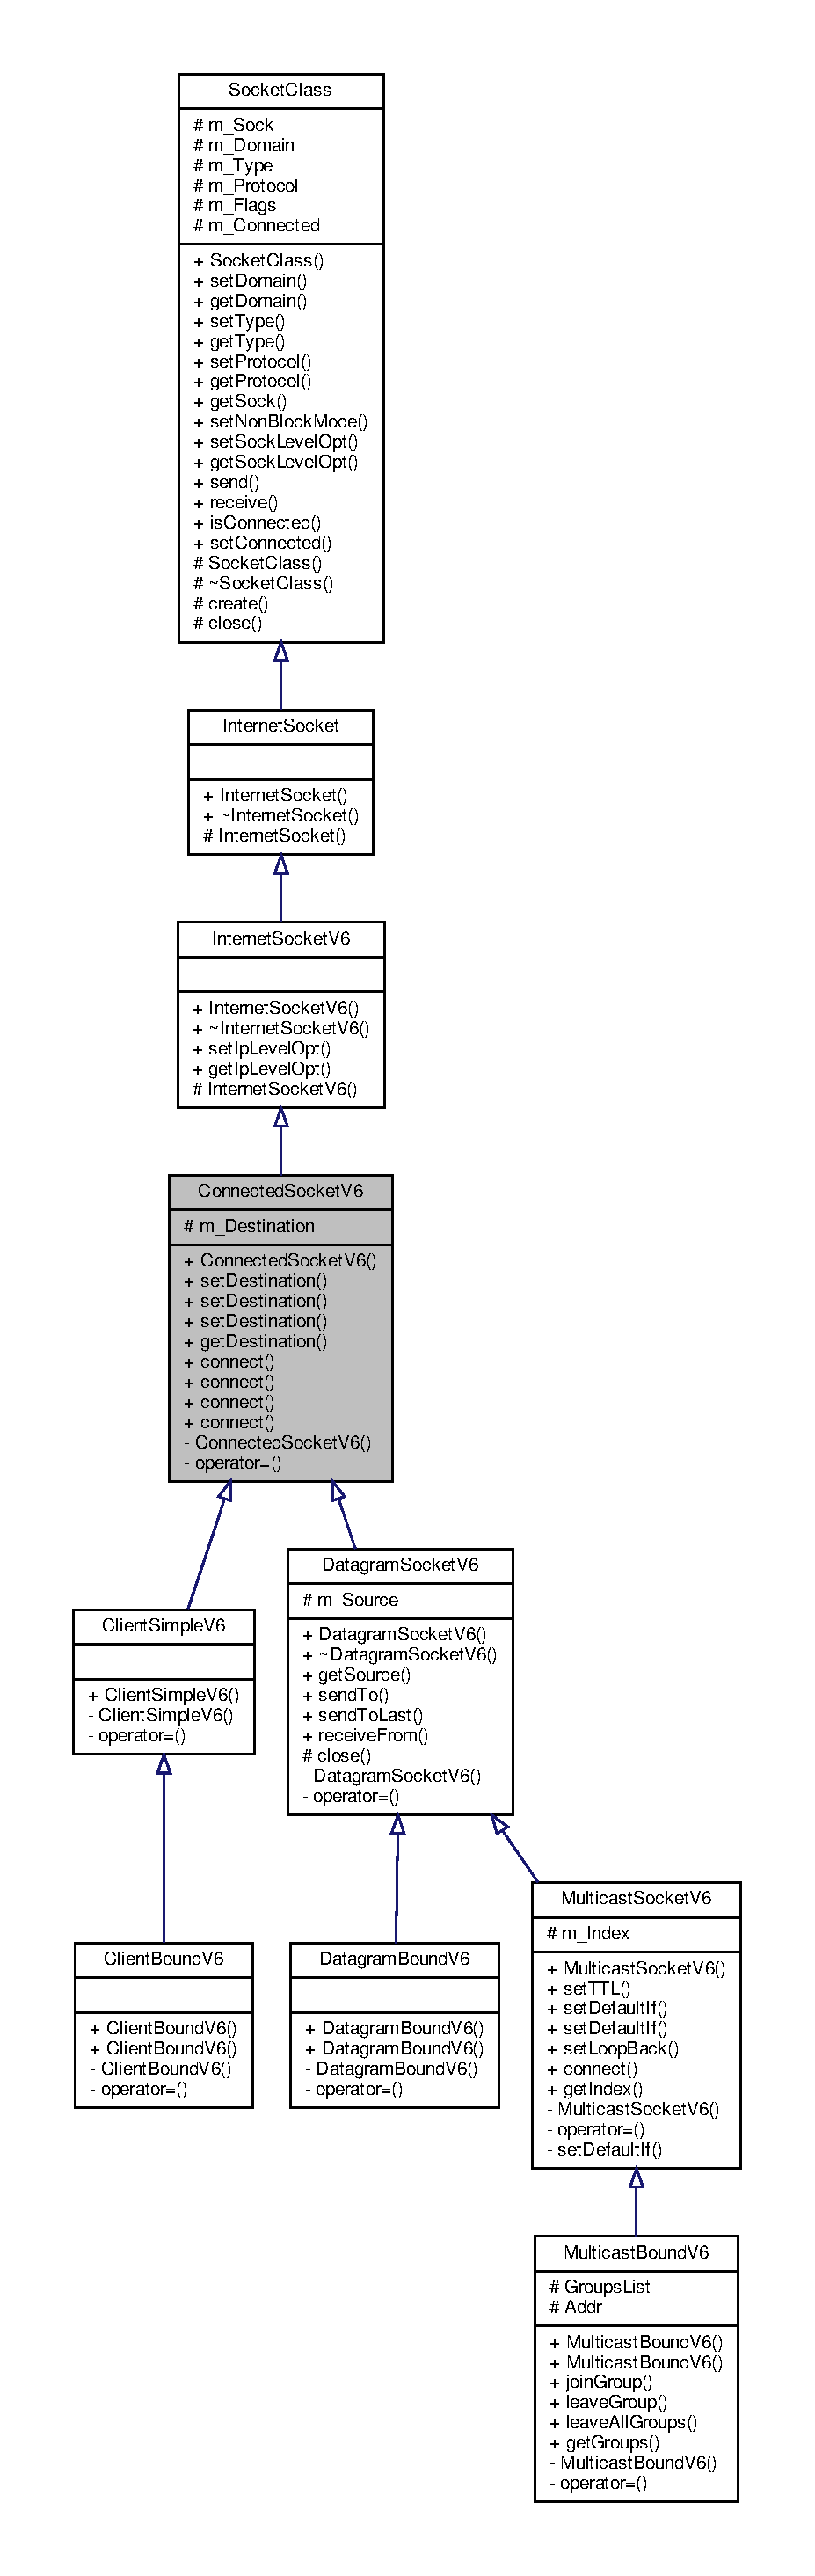
\includegraphics[height=550pt]{classConnectedSocketV6__inherit__graph}
\end{center}
\end{figure}
\subsection*{Public Member Functions}
\begin{DoxyCompactItemize}
\item 
\hyperlink{classConnectedSocketV6_a3669db7a7ad6af9824f56d1565b86889}{Connected\+Socket\+V6} ()
\item 
void \hyperlink{classConnectedSocketV6_ac95a20c1700d3a95b83c253c695f9838}{set\+Destination} (sockaddr\+\_\+in6 Dest)
\item 
void \hyperlink{classConnectedSocketV6_aa4f9dd426ff72420bdd315a9668d2139}{set\+Destination} (in6\+\_\+addr Address, short Port)
\item 
void \hyperlink{classConnectedSocketV6_aefa8952aeb0d63332c4afcd5538b118e}{set\+Destination} (const char $\ast$Address, short Port)
\item 
sockaddr\+\_\+in6 \& \hyperlink{classConnectedSocketV6_a113422dc7ea93e8abfaecbfe4763a260}{get\+Destination} ()
\item 
virtual void \hyperlink{classConnectedSocketV6_ad08bcbb9f35ac5c5693e352d1bbc5460}{connect} ()
\item 
void \hyperlink{classConnectedSocketV6_adfdf319dc49b3ff8cb2507178dfeda3f}{connect} (in6\+\_\+addr Address, short Port)
\item 
void \hyperlink{classConnectedSocketV6_a9b3101138e8dc3df9a70fd3a8d325a8a}{connect} (const char $\ast$Address, short Port)
\item 
void \hyperlink{classConnectedSocketV6_a2f93ef688800a0631eae284661c08368}{connect} (sockaddr\+\_\+in6 Dest)
\end{DoxyCompactItemize}
\subsection*{Protected Attributes}
\begin{DoxyCompactItemize}
\item 
sockaddr\+\_\+in6 \hyperlink{classConnectedSocketV6_ab05802f2cded1638b11541be1e78942c}{m\+\_\+\+Destination}
\begin{DoxyCompactList}\small\item\em Destination endpoint properties. \end{DoxyCompactList}\end{DoxyCompactItemize}
\subsection*{Private Member Functions}
\begin{DoxyCompactItemize}
\item 
\hyperlink{classConnectedSocketV6_ad4936b91c36fca90b65a995145a68692}{Connected\+Socket\+V6} (\hyperlink{classConnectedSocketV6}{Connected\+Socket\+V6} \&s)
\item 
\hyperlink{classConnectedSocketV6}{Connected\+Socket\+V6} \& \hyperlink{classConnectedSocketV6_a75cc4a8c5c0d52167e652eccac12859b}{operator=} (\hyperlink{classConnectedSocketV6}{Connected\+Socket\+V6} \&s)
\end{DoxyCompactItemize}
\subsection*{Additional Inherited Members}


\subsection{Detailed Description}
Socket that can connect to another. 

\subsection{Constructor \& Destructor Documentation}
\mbox{\Hypertarget{classConnectedSocketV6_a3669db7a7ad6af9824f56d1565b86889}\label{classConnectedSocketV6_a3669db7a7ad6af9824f56d1565b86889}} 
\index{Connected\+Socket\+V6@{Connected\+Socket\+V6}!Connected\+Socket\+V6@{Connected\+Socket\+V6}}
\index{Connected\+Socket\+V6@{Connected\+Socket\+V6}!Connected\+Socket\+V6@{Connected\+Socket\+V6}}
\subsubsection{\texorpdfstring{Connected\+Socket\+V6()}{ConnectedSocketV6()}\hspace{0.1cm}{\footnotesize\ttfamily [1/2]}}
{\footnotesize\ttfamily Connected\+Socket\+V6\+::\+Connected\+Socket\+V6 (\begin{DoxyParamCaption}{ }\end{DoxyParamCaption})\hspace{0.3cm}{\ttfamily [inline]}}

Constructor. Default constructor. \mbox{\Hypertarget{classConnectedSocketV6_ad4936b91c36fca90b65a995145a68692}\label{classConnectedSocketV6_ad4936b91c36fca90b65a995145a68692}} 
\index{Connected\+Socket\+V6@{Connected\+Socket\+V6}!Connected\+Socket\+V6@{Connected\+Socket\+V6}}
\index{Connected\+Socket\+V6@{Connected\+Socket\+V6}!Connected\+Socket\+V6@{Connected\+Socket\+V6}}
\subsubsection{\texorpdfstring{Connected\+Socket\+V6()}{ConnectedSocketV6()}\hspace{0.1cm}{\footnotesize\ttfamily [2/2]}}
{\footnotesize\ttfamily Connected\+Socket\+V6\+::\+Connected\+Socket\+V6 (\begin{DoxyParamCaption}\item[{\hyperlink{classConnectedSocketV6}{Connected\+Socket\+V6} \&}]{s }\end{DoxyParamCaption})\hspace{0.3cm}{\ttfamily [private]}}

Copy constructor. Makes the class uncopyable . 

\subsection{Member Function Documentation}
\mbox{\Hypertarget{classConnectedSocketV6_ad08bcbb9f35ac5c5693e352d1bbc5460}\label{classConnectedSocketV6_ad08bcbb9f35ac5c5693e352d1bbc5460}} 
\index{Connected\+Socket\+V6@{Connected\+Socket\+V6}!connect@{connect}}
\index{connect@{connect}!Connected\+Socket\+V6@{Connected\+Socket\+V6}}
\subsubsection{\texorpdfstring{connect()}{connect()}\hspace{0.1cm}{\footnotesize\ttfamily [1/4]}}
{\footnotesize\ttfamily void Connected\+Socket\+V6\+::connect (\begin{DoxyParamCaption}{ }\end{DoxyParamCaption})\hspace{0.3cm}{\ttfamily [virtual]}}

Connect to destination endpoint. 
\begin{DoxyExceptions}{Exceptions}
{\em Sock\+Exception.} & \\
\hline
\end{DoxyExceptions}


Reimplemented in \hyperlink{classMulticastSocketV6_a81b62a13aff687c5b94b8f8a946c58ed}{Multicast\+Socket\+V6}.

\mbox{\Hypertarget{classConnectedSocketV6_adfdf319dc49b3ff8cb2507178dfeda3f}\label{classConnectedSocketV6_adfdf319dc49b3ff8cb2507178dfeda3f}} 
\index{Connected\+Socket\+V6@{Connected\+Socket\+V6}!connect@{connect}}
\index{connect@{connect}!Connected\+Socket\+V6@{Connected\+Socket\+V6}}
\subsubsection{\texorpdfstring{connect()}{connect()}\hspace{0.1cm}{\footnotesize\ttfamily [2/4]}}
{\footnotesize\ttfamily void Connected\+Socket\+V6\+::connect (\begin{DoxyParamCaption}\item[{in6\+\_\+addr}]{Address,  }\item[{short}]{Port }\end{DoxyParamCaption})\hspace{0.3cm}{\ttfamily [inline]}}

Connect to destination endpoint. 
\begin{DoxyParams}{Parameters}
{\em Address} & \+: I\+Pv6 address structure. \\
\hline
{\em Port} & \+: port number in network byte order. \\
\hline
\end{DoxyParams}

\begin{DoxyExceptions}{Exceptions}
{\em Sock\+Exception.} & \\
\hline
\end{DoxyExceptions}
\mbox{\Hypertarget{classConnectedSocketV6_a9b3101138e8dc3df9a70fd3a8d325a8a}\label{classConnectedSocketV6_a9b3101138e8dc3df9a70fd3a8d325a8a}} 
\index{Connected\+Socket\+V6@{Connected\+Socket\+V6}!connect@{connect}}
\index{connect@{connect}!Connected\+Socket\+V6@{Connected\+Socket\+V6}}
\subsubsection{\texorpdfstring{connect()}{connect()}\hspace{0.1cm}{\footnotesize\ttfamily [3/4]}}
{\footnotesize\ttfamily void Connected\+Socket\+V6\+::connect (\begin{DoxyParamCaption}\item[{const char $\ast$}]{Address,  }\item[{short}]{Port }\end{DoxyParamCaption})\hspace{0.3cm}{\ttfamily [inline]}}

Connect to destination endpoint. 
\begin{DoxyParams}{Parameters}
{\em Address} & \+: I\+Pv6 address in textual notation. \\
\hline
{\em Port} & \+: port number in network byte order. \\
\hline
\end{DoxyParams}

\begin{DoxyExceptions}{Exceptions}
{\em Sock\+Exception.} & \\
\hline
\end{DoxyExceptions}
\mbox{\Hypertarget{classConnectedSocketV6_a2f93ef688800a0631eae284661c08368}\label{classConnectedSocketV6_a2f93ef688800a0631eae284661c08368}} 
\index{Connected\+Socket\+V6@{Connected\+Socket\+V6}!connect@{connect}}
\index{connect@{connect}!Connected\+Socket\+V6@{Connected\+Socket\+V6}}
\subsubsection{\texorpdfstring{connect()}{connect()}\hspace{0.1cm}{\footnotesize\ttfamily [4/4]}}
{\footnotesize\ttfamily void Connected\+Socket\+V6\+::connect (\begin{DoxyParamCaption}\item[{sockaddr\+\_\+in6}]{Dest }\end{DoxyParamCaption})\hspace{0.3cm}{\ttfamily [inline]}}

Connect to destination endpoint. 
\begin{DoxyParams}{Parameters}
{\em Dest} & \+: sockaddr\+\_\+in6 structure filled with destination endpoint properties. \\
\hline
\end{DoxyParams}

\begin{DoxyExceptions}{Exceptions}
{\em Sock\+Exception.} & \\
\hline
\end{DoxyExceptions}
\mbox{\Hypertarget{classConnectedSocketV6_a113422dc7ea93e8abfaecbfe4763a260}\label{classConnectedSocketV6_a113422dc7ea93e8abfaecbfe4763a260}} 
\index{Connected\+Socket\+V6@{Connected\+Socket\+V6}!get\+Destination@{get\+Destination}}
\index{get\+Destination@{get\+Destination}!Connected\+Socket\+V6@{Connected\+Socket\+V6}}
\subsubsection{\texorpdfstring{get\+Destination()}{getDestination()}}
{\footnotesize\ttfamily sockaddr\+\_\+in6\& Connected\+Socket\+V6\+::get\+Destination (\begin{DoxyParamCaption}{ }\end{DoxyParamCaption})\hspace{0.3cm}{\ttfamily [inline]}}

Deliver destination endpoint properties. \begin{DoxyReturn}{Returns}
sockaddr\+\_\+in structure filled with endpoint properties. 
\end{DoxyReturn}
\mbox{\Hypertarget{classConnectedSocketV6_a75cc4a8c5c0d52167e652eccac12859b}\label{classConnectedSocketV6_a75cc4a8c5c0d52167e652eccac12859b}} 
\index{Connected\+Socket\+V6@{Connected\+Socket\+V6}!operator=@{operator=}}
\index{operator=@{operator=}!Connected\+Socket\+V6@{Connected\+Socket\+V6}}
\subsubsection{\texorpdfstring{operator=()}{operator=()}}
{\footnotesize\ttfamily \hyperlink{classConnectedSocketV6}{Connected\+Socket\+V6}\& Connected\+Socket\+V6\+::operator= (\begin{DoxyParamCaption}\item[{\hyperlink{classConnectedSocketV6}{Connected\+Socket\+V6} \&}]{s }\end{DoxyParamCaption})\hspace{0.3cm}{\ttfamily [private]}}

Operator assign. Makes the class uncopyable . \mbox{\Hypertarget{classConnectedSocketV6_ac95a20c1700d3a95b83c253c695f9838}\label{classConnectedSocketV6_ac95a20c1700d3a95b83c253c695f9838}} 
\index{Connected\+Socket\+V6@{Connected\+Socket\+V6}!set\+Destination@{set\+Destination}}
\index{set\+Destination@{set\+Destination}!Connected\+Socket\+V6@{Connected\+Socket\+V6}}
\subsubsection{\texorpdfstring{set\+Destination()}{setDestination()}\hspace{0.1cm}{\footnotesize\ttfamily [1/3]}}
{\footnotesize\ttfamily void Connected\+Socket\+V6\+::set\+Destination (\begin{DoxyParamCaption}\item[{sockaddr\+\_\+in6}]{Dest }\end{DoxyParamCaption})\hspace{0.3cm}{\ttfamily [inline]}}

Set connection destination endpoint. 
\begin{DoxyParams}{Parameters}
{\em Dest} & \+: sockaddr\+\_\+in6 structure filled with destination endpoint properties. \\
\hline
\end{DoxyParams}
\mbox{\Hypertarget{classConnectedSocketV6_aa4f9dd426ff72420bdd315a9668d2139}\label{classConnectedSocketV6_aa4f9dd426ff72420bdd315a9668d2139}} 
\index{Connected\+Socket\+V6@{Connected\+Socket\+V6}!set\+Destination@{set\+Destination}}
\index{set\+Destination@{set\+Destination}!Connected\+Socket\+V6@{Connected\+Socket\+V6}}
\subsubsection{\texorpdfstring{set\+Destination()}{setDestination()}\hspace{0.1cm}{\footnotesize\ttfamily [2/3]}}
{\footnotesize\ttfamily void Connected\+Socket\+V6\+::set\+Destination (\begin{DoxyParamCaption}\item[{in6\+\_\+addr}]{Address,  }\item[{short}]{Port }\end{DoxyParamCaption})}

Set connection destination endpoint. 
\begin{DoxyParams}{Parameters}
{\em Address} & \+: I\+Pv6 address structure. \\
\hline
{\em Port} & \+: port number in network byte order. \\
\hline
\end{DoxyParams}
\mbox{\Hypertarget{classConnectedSocketV6_aefa8952aeb0d63332c4afcd5538b118e}\label{classConnectedSocketV6_aefa8952aeb0d63332c4afcd5538b118e}} 
\index{Connected\+Socket\+V6@{Connected\+Socket\+V6}!set\+Destination@{set\+Destination}}
\index{set\+Destination@{set\+Destination}!Connected\+Socket\+V6@{Connected\+Socket\+V6}}
\subsubsection{\texorpdfstring{set\+Destination()}{setDestination()}\hspace{0.1cm}{\footnotesize\ttfamily [3/3]}}
{\footnotesize\ttfamily void Connected\+Socket\+V6\+::set\+Destination (\begin{DoxyParamCaption}\item[{const char $\ast$}]{Address,  }\item[{short}]{Port }\end{DoxyParamCaption})}

Set connection destination endpoint. 
\begin{DoxyParams}{Parameters}
{\em Address} & \+: I\+Pv6 address in textual notation. \\
\hline
{\em Port} & \+: port number in network byte order. \\
\hline
\end{DoxyParams}


\subsection{Member Data Documentation}
\mbox{\Hypertarget{classConnectedSocketV6_ab05802f2cded1638b11541be1e78942c}\label{classConnectedSocketV6_ab05802f2cded1638b11541be1e78942c}} 
\index{Connected\+Socket\+V6@{Connected\+Socket\+V6}!m\+\_\+\+Destination@{m\+\_\+\+Destination}}
\index{m\+\_\+\+Destination@{m\+\_\+\+Destination}!Connected\+Socket\+V6@{Connected\+Socket\+V6}}
\subsubsection{\texorpdfstring{m\+\_\+\+Destination}{m\_Destination}}
{\footnotesize\ttfamily sockaddr\+\_\+in6 Connected\+Socket\+V6\+::m\+\_\+\+Destination\hspace{0.3cm}{\ttfamily [protected]}}



Destination endpoint properties. 



The documentation for this class was generated from the following files\+:\begin{DoxyCompactItemize}
\item 
\hyperlink{ConnectedSocketV6_8h}{Connected\+Socket\+V6.\+h}\item 
\hyperlink{ConnectedSocketV6_8cpp}{Connected\+Socket\+V6.\+cpp}\end{DoxyCompactItemize}

\hypertarget{classDatagramBound}{}\section{Datagram\+Bound Class Reference}
\label{classDatagramBound}\index{Datagram\+Bound@{Datagram\+Bound}}


U\+DP socket bound to specified port and address (aka U\+DP server).  




{\ttfamily \#include $<$Datagram\+Bound.\+h$>$}



Inheritance diagram for Datagram\+Bound\+:\nopagebreak
\begin{figure}[H]
\begin{center}
\leavevmode
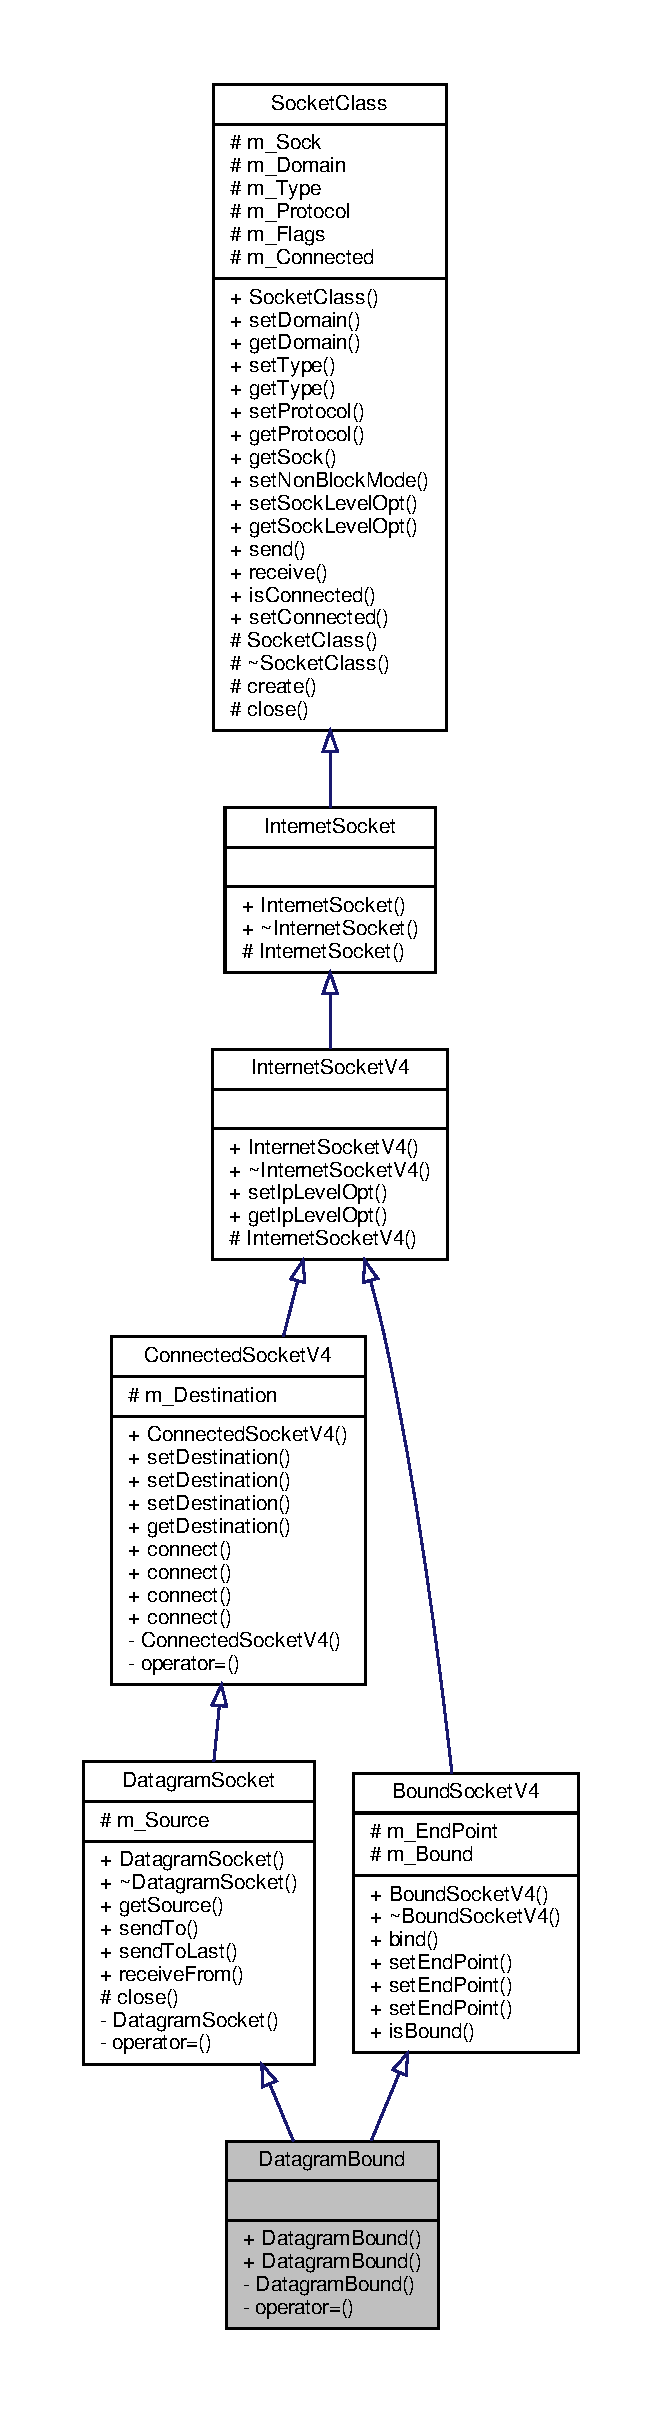
\includegraphics[height=550pt]{classDatagramBound__inherit__graph}
\end{center}
\end{figure}
\subsection*{Public Member Functions}
\begin{DoxyCompactItemize}
\item 
\hyperlink{classDatagramBound_a0a4b53fd787e0c1e038484917655397f}{Datagram\+Bound} (short Port, in\+\_\+addr\+\_\+t Address=I\+N\+A\+D\+D\+R\+\_\+\+A\+NY)
\item 
\hyperlink{classDatagramBound_acc69d2a4bb9bac09b98fec275cc81780}{Datagram\+Bound} (short Port, const char $\ast$Address)
\end{DoxyCompactItemize}
\subsection*{Private Member Functions}
\begin{DoxyCompactItemize}
\item 
\hyperlink{classDatagramBound_a834acb4cd0993871974a6069dceafe9c}{Datagram\+Bound} (\hyperlink{classDatagramBound}{Datagram\+Bound} \&d)
\item 
\hyperlink{classDatagramBound}{Datagram\+Bound} \& \hyperlink{classDatagramBound_a2b499dba8e0be3618e45b75232e050d0}{operator=} (\hyperlink{classDatagramBound}{Datagram\+Bound} \&d)
\end{DoxyCompactItemize}
\subsection*{Additional Inherited Members}


\subsection{Detailed Description}
U\+DP socket bound to specified port and address (aka U\+DP server). 

\subsection{Constructor \& Destructor Documentation}
\mbox{\Hypertarget{classDatagramBound_a0a4b53fd787e0c1e038484917655397f}\label{classDatagramBound_a0a4b53fd787e0c1e038484917655397f}} 
\index{Datagram\+Bound@{Datagram\+Bound}!Datagram\+Bound@{Datagram\+Bound}}
\index{Datagram\+Bound@{Datagram\+Bound}!Datagram\+Bound@{Datagram\+Bound}}
\subsubsection{\texorpdfstring{Datagram\+Bound()}{DatagramBound()}\hspace{0.1cm}{\footnotesize\ttfamily [1/3]}}
{\footnotesize\ttfamily Datagram\+Bound\+::\+Datagram\+Bound (\begin{DoxyParamCaption}\item[{short}]{Port,  }\item[{in\+\_\+addr\+\_\+t}]{Address = {\ttfamily INADDR\+\_\+ANY} }\end{DoxyParamCaption})}

Constructor. 
\begin{DoxyParams}{Parameters}
{\em Port} & \+: port number for bind in network byte order. \\
\hline
{\em Address} & \+: I\+Pv4 address for bind in network byte order. \\
\hline
\end{DoxyParams}

\begin{DoxyExceptions}{Exceptions}
{\em Sock\+Exception.} & \\
\hline
\end{DoxyExceptions}
\mbox{\Hypertarget{classDatagramBound_acc69d2a4bb9bac09b98fec275cc81780}\label{classDatagramBound_acc69d2a4bb9bac09b98fec275cc81780}} 
\index{Datagram\+Bound@{Datagram\+Bound}!Datagram\+Bound@{Datagram\+Bound}}
\index{Datagram\+Bound@{Datagram\+Bound}!Datagram\+Bound@{Datagram\+Bound}}
\subsubsection{\texorpdfstring{Datagram\+Bound()}{DatagramBound()}\hspace{0.1cm}{\footnotesize\ttfamily [2/3]}}
{\footnotesize\ttfamily Datagram\+Bound\+::\+Datagram\+Bound (\begin{DoxyParamCaption}\item[{short}]{Port,  }\item[{const char $\ast$}]{Address }\end{DoxyParamCaption})}

Constructor. 
\begin{DoxyParams}{Parameters}
{\em Port} & \+: port number for bind in network byte order. \\
\hline
{\em Address} & \+: I\+Pv4 address for bind in decimal dot notation. \\
\hline
\end{DoxyParams}

\begin{DoxyExceptions}{Exceptions}
{\em Sock\+Exception.} & \\
\hline
\end{DoxyExceptions}
\mbox{\Hypertarget{classDatagramBound_a834acb4cd0993871974a6069dceafe9c}\label{classDatagramBound_a834acb4cd0993871974a6069dceafe9c}} 
\index{Datagram\+Bound@{Datagram\+Bound}!Datagram\+Bound@{Datagram\+Bound}}
\index{Datagram\+Bound@{Datagram\+Bound}!Datagram\+Bound@{Datagram\+Bound}}
\subsubsection{\texorpdfstring{Datagram\+Bound()}{DatagramBound()}\hspace{0.1cm}{\footnotesize\ttfamily [3/3]}}
{\footnotesize\ttfamily Datagram\+Bound\+::\+Datagram\+Bound (\begin{DoxyParamCaption}\item[{\hyperlink{classDatagramBound}{Datagram\+Bound} \&}]{d }\end{DoxyParamCaption})\hspace{0.3cm}{\ttfamily [private]}}

Copy constructor. Makes the class uncopyable. 

\subsection{Member Function Documentation}
\mbox{\Hypertarget{classDatagramBound_a2b499dba8e0be3618e45b75232e050d0}\label{classDatagramBound_a2b499dba8e0be3618e45b75232e050d0}} 
\index{Datagram\+Bound@{Datagram\+Bound}!operator=@{operator=}}
\index{operator=@{operator=}!Datagram\+Bound@{Datagram\+Bound}}
\subsubsection{\texorpdfstring{operator=()}{operator=()}}
{\footnotesize\ttfamily \hyperlink{classDatagramBound}{Datagram\+Bound}\& Datagram\+Bound\+::operator= (\begin{DoxyParamCaption}\item[{\hyperlink{classDatagramBound}{Datagram\+Bound} \&}]{d }\end{DoxyParamCaption})\hspace{0.3cm}{\ttfamily [private]}}

Operator assign. Makes the class uncopyable. 

The documentation for this class was generated from the following files\+:\begin{DoxyCompactItemize}
\item 
\hyperlink{DatagramBound_8h}{Datagram\+Bound.\+h}\item 
\hyperlink{DatagramBound_8cpp}{Datagram\+Bound.\+cpp}\end{DoxyCompactItemize}

\hypertarget{classDatagramBoundV6}{}\section{Datagram\+Bound\+V6 Class Reference}
\label{classDatagramBoundV6}\index{Datagram\+Bound\+V6@{Datagram\+Bound\+V6}}


U\+DP socket bound to specified port and address (aka U\+DP server) for I\+Pv6.  




{\ttfamily \#include $<$Datagram\+Bound\+V6.\+h$>$}



Inheritance diagram for Datagram\+Bound\+V6\+:\nopagebreak
\begin{figure}[H]
\begin{center}
\leavevmode
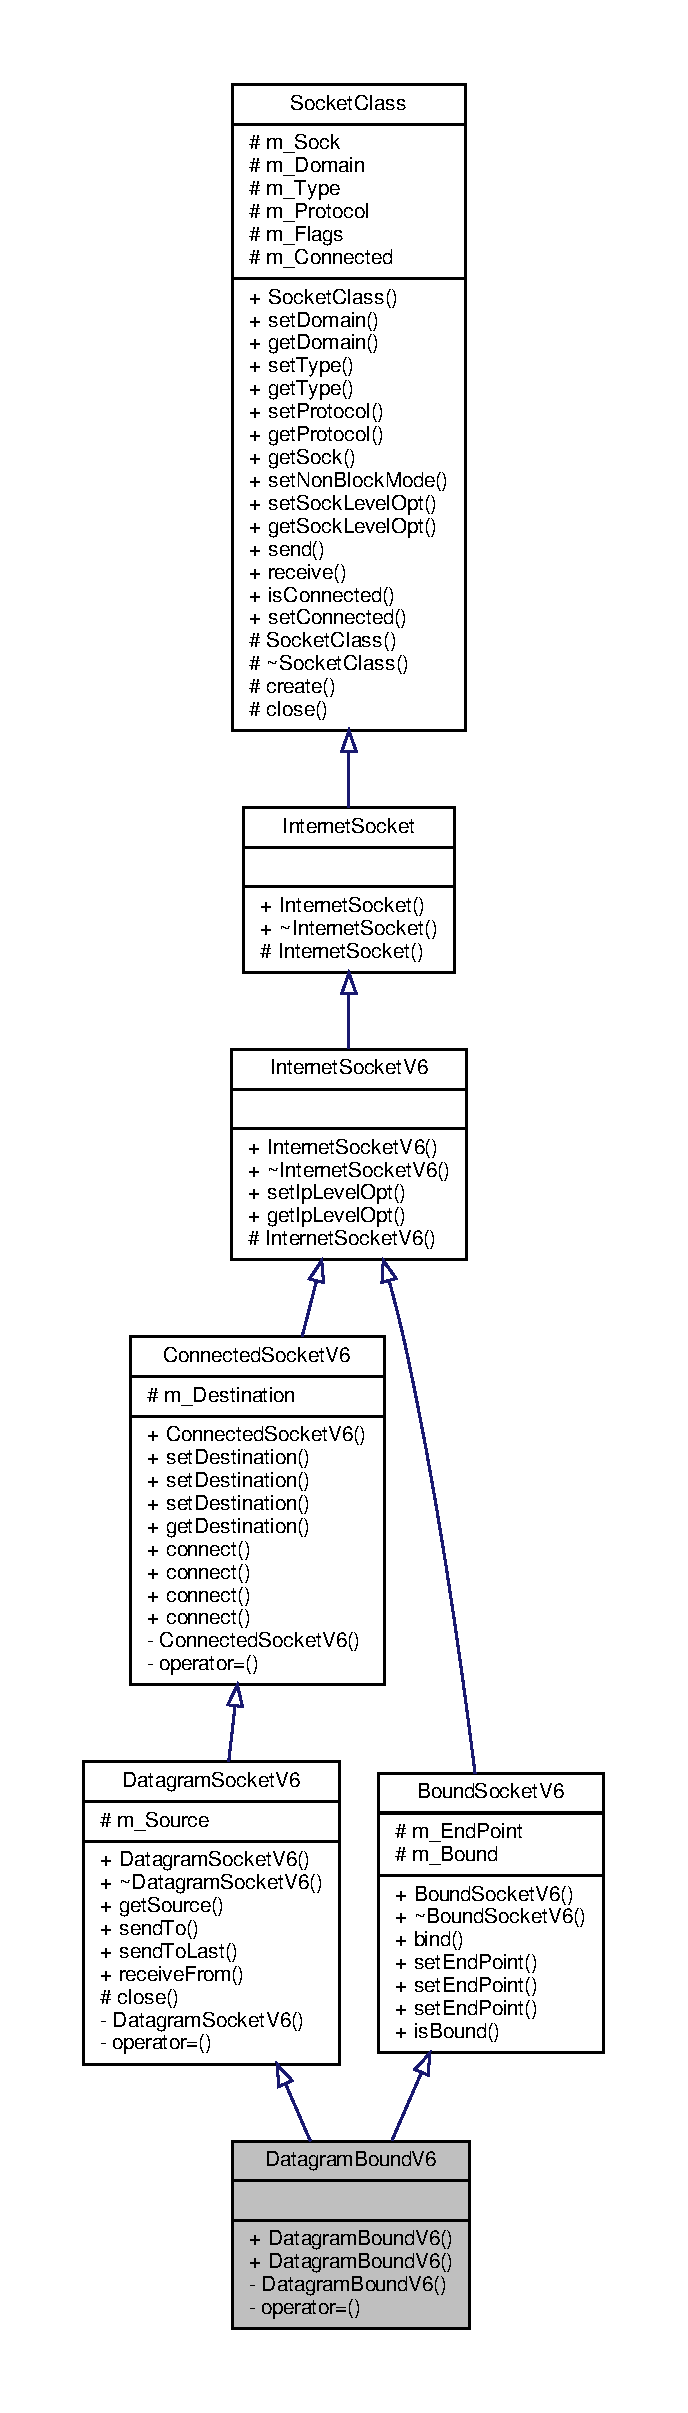
\includegraphics[height=550pt]{classDatagramBoundV6__inherit__graph}
\end{center}
\end{figure}
\subsection*{Public Member Functions}
\begin{DoxyCompactItemize}
\item 
\hyperlink{classDatagramBoundV6_a2ea297627599924828a2ba5f3841f5b6}{Datagram\+Bound\+V6} (short Port, in6\+\_\+addr Address=in6addr\+\_\+any)
\item 
\hyperlink{classDatagramBoundV6_a10466ff587a48113bafaedfd6fe7b0be}{Datagram\+Bound\+V6} (short Port, const char $\ast$Address)
\end{DoxyCompactItemize}
\subsection*{Private Member Functions}
\begin{DoxyCompactItemize}
\item 
\hyperlink{classDatagramBoundV6_ac392602b5e9fa32a4ef137e97ddc0842}{Datagram\+Bound\+V6} (\hyperlink{classDatagramBoundV6}{Datagram\+Bound\+V6} \&d)
\item 
\hyperlink{classDatagramBoundV6}{Datagram\+Bound\+V6} \& \hyperlink{classDatagramBoundV6_ad4e4d9bf21708ecb03786df5230bd769}{operator=} (\hyperlink{classDatagramBoundV6}{Datagram\+Bound\+V6} \&d)
\end{DoxyCompactItemize}
\subsection*{Additional Inherited Members}


\subsection{Detailed Description}
U\+DP socket bound to specified port and address (aka U\+DP server) for I\+Pv6. 

\subsection{Constructor \& Destructor Documentation}
\mbox{\Hypertarget{classDatagramBoundV6_a2ea297627599924828a2ba5f3841f5b6}\label{classDatagramBoundV6_a2ea297627599924828a2ba5f3841f5b6}} 
\index{Datagram\+Bound\+V6@{Datagram\+Bound\+V6}!Datagram\+Bound\+V6@{Datagram\+Bound\+V6}}
\index{Datagram\+Bound\+V6@{Datagram\+Bound\+V6}!Datagram\+Bound\+V6@{Datagram\+Bound\+V6}}
\subsubsection{\texorpdfstring{Datagram\+Bound\+V6()}{DatagramBoundV6()}\hspace{0.1cm}{\footnotesize\ttfamily [1/3]}}
{\footnotesize\ttfamily Datagram\+Bound\+V6\+::\+Datagram\+Bound\+V6 (\begin{DoxyParamCaption}\item[{short}]{Port,  }\item[{in6\+\_\+addr}]{Address = {\ttfamily in6addr\+\_\+any} }\end{DoxyParamCaption})}

Constructor. 
\begin{DoxyParams}{Parameters}
{\em Port} & \+: port number for bind in network byte order. \\
\hline
{\em Address} & \+: I\+Pv6 address for bind in network byte order. \\
\hline
\end{DoxyParams}

\begin{DoxyExceptions}{Exceptions}
{\em Sock\+Exception.} & \\
\hline
\end{DoxyExceptions}
\mbox{\Hypertarget{classDatagramBoundV6_a10466ff587a48113bafaedfd6fe7b0be}\label{classDatagramBoundV6_a10466ff587a48113bafaedfd6fe7b0be}} 
\index{Datagram\+Bound\+V6@{Datagram\+Bound\+V6}!Datagram\+Bound\+V6@{Datagram\+Bound\+V6}}
\index{Datagram\+Bound\+V6@{Datagram\+Bound\+V6}!Datagram\+Bound\+V6@{Datagram\+Bound\+V6}}
\subsubsection{\texorpdfstring{Datagram\+Bound\+V6()}{DatagramBoundV6()}\hspace{0.1cm}{\footnotesize\ttfamily [2/3]}}
{\footnotesize\ttfamily Datagram\+Bound\+V6\+::\+Datagram\+Bound\+V6 (\begin{DoxyParamCaption}\item[{short}]{Port,  }\item[{const char $\ast$}]{Address }\end{DoxyParamCaption})}

Constructor. 
\begin{DoxyParams}{Parameters}
{\em Port} & \+: port number for bind in network byte order. \\
\hline
{\em Address} & \+: I\+Pv6 address for bind in textual notation. \\
\hline
\end{DoxyParams}

\begin{DoxyExceptions}{Exceptions}
{\em Sock\+Exception.} & \\
\hline
\end{DoxyExceptions}
\mbox{\Hypertarget{classDatagramBoundV6_ac392602b5e9fa32a4ef137e97ddc0842}\label{classDatagramBoundV6_ac392602b5e9fa32a4ef137e97ddc0842}} 
\index{Datagram\+Bound\+V6@{Datagram\+Bound\+V6}!Datagram\+Bound\+V6@{Datagram\+Bound\+V6}}
\index{Datagram\+Bound\+V6@{Datagram\+Bound\+V6}!Datagram\+Bound\+V6@{Datagram\+Bound\+V6}}
\subsubsection{\texorpdfstring{Datagram\+Bound\+V6()}{DatagramBoundV6()}\hspace{0.1cm}{\footnotesize\ttfamily [3/3]}}
{\footnotesize\ttfamily Datagram\+Bound\+V6\+::\+Datagram\+Bound\+V6 (\begin{DoxyParamCaption}\item[{\hyperlink{classDatagramBoundV6}{Datagram\+Bound\+V6} \&}]{d }\end{DoxyParamCaption})\hspace{0.3cm}{\ttfamily [private]}}

Copy constructor. Makes the class uncopyable. 

\subsection{Member Function Documentation}
\mbox{\Hypertarget{classDatagramBoundV6_ad4e4d9bf21708ecb03786df5230bd769}\label{classDatagramBoundV6_ad4e4d9bf21708ecb03786df5230bd769}} 
\index{Datagram\+Bound\+V6@{Datagram\+Bound\+V6}!operator=@{operator=}}
\index{operator=@{operator=}!Datagram\+Bound\+V6@{Datagram\+Bound\+V6}}
\subsubsection{\texorpdfstring{operator=()}{operator=()}}
{\footnotesize\ttfamily \hyperlink{classDatagramBoundV6}{Datagram\+Bound\+V6}\& Datagram\+Bound\+V6\+::operator= (\begin{DoxyParamCaption}\item[{\hyperlink{classDatagramBoundV6}{Datagram\+Bound\+V6} \&}]{d }\end{DoxyParamCaption})\hspace{0.3cm}{\ttfamily [private]}}

Operator assign. Makes the class uncopyable. 

The documentation for this class was generated from the following files\+:\begin{DoxyCompactItemize}
\item 
\hyperlink{DatagramBoundV6_8h}{Datagram\+Bound\+V6.\+h}\item 
\hyperlink{DatagramBoundV6_8cpp}{Datagram\+Bound\+V6.\+cpp}\end{DoxyCompactItemize}

\hypertarget{classDatagramSocket}{}\section{Datagram\+Socket Class Reference}
\label{classDatagramSocket}\index{Datagram\+Socket@{Datagram\+Socket}}


Class for U\+DP sockets.  




{\ttfamily \#include $<$Datagram\+Socket.\+h$>$}



Inheritance diagram for Datagram\+Socket\+:\nopagebreak
\begin{figure}[H]
\begin{center}
\leavevmode
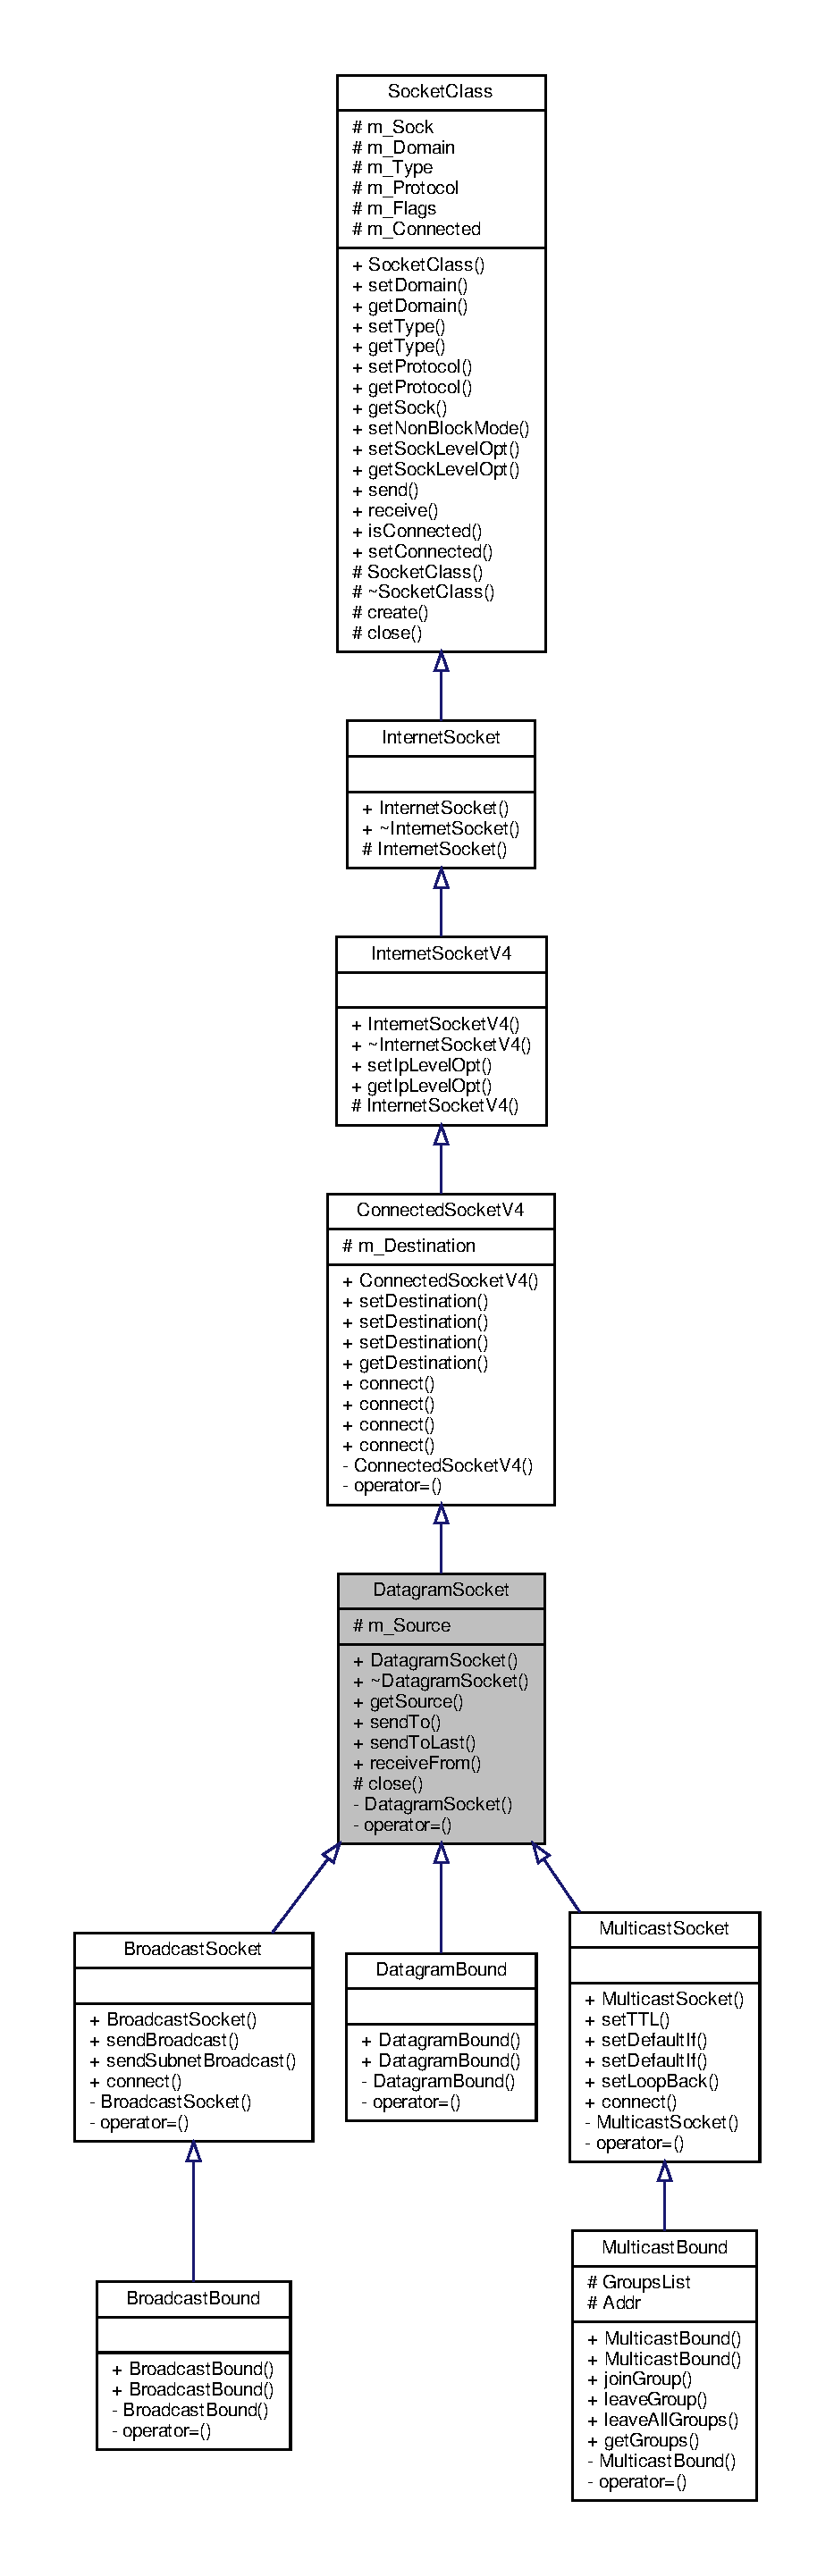
\includegraphics[height=550pt]{classDatagramSocket__inherit__graph}
\end{center}
\end{figure}
\subsection*{Public Member Functions}
\begin{DoxyCompactItemize}
\item 
\hyperlink{classDatagramSocket_a154493cb7278a67055b303aed93c4272}{Datagram\+Socket} (int protocol=0)
\item 
virtual \hyperlink{classDatagramSocket_a749202f672a5c649ef1b3efee31cbe64}{$\sim$\+Datagram\+Socket} ()
\begin{DoxyCompactList}\small\item\em Destructor. \end{DoxyCompactList}\item 
sockaddr\+\_\+in \& \hyperlink{classDatagramSocket_a3ab11d022387bea4f04d8bd2385d6560}{get\+Source} ()
\item 
int \hyperlink{classDatagramSocket_a85adaaa4c3a7ecf4259c4608a7d02de4}{send\+To} (const void $\ast$Buffer, size\+\_\+t Length, int Flags=0)
\item 
int \hyperlink{classDatagramSocket_a74cdf74e62415895600df98a5115826a}{send\+To\+Last} (const void $\ast$Buffer, size\+\_\+t Length, int Flags=0)
\item 
int \hyperlink{classDatagramSocket_a0366888764a76a89db65f61795e55c07}{receive\+From} (void $\ast$Buffer, size\+\_\+t Length, int Flags=0)
\end{DoxyCompactItemize}
\subsection*{Protected Member Functions}
\begin{DoxyCompactItemize}
\item 
virtual void \hyperlink{classDatagramSocket_a5c926c1d93a9e1b2e19d73170c4984cb}{close} ()
\begin{DoxyCompactList}\small\item\em Close socket. \end{DoxyCompactList}\end{DoxyCompactItemize}
\subsection*{Protected Attributes}
\begin{DoxyCompactItemize}
\item 
sockaddr\+\_\+in \hyperlink{classDatagramSocket_a1b7784d4356ad11fdb109c44c5b227ab}{m\+\_\+\+Source}
\begin{DoxyCompactList}\small\item\em Properties of the endpoint, that last received datagram was send from. \end{DoxyCompactList}\end{DoxyCompactItemize}
\subsection*{Private Member Functions}
\begin{DoxyCompactItemize}
\item 
\hyperlink{classDatagramSocket_a46a9ca425d2204ab613a28c090f289cb}{Datagram\+Socket} (\hyperlink{classDatagramSocket}{Datagram\+Socket} \&d)
\item 
\hyperlink{classDatagramSocket}{Datagram\+Socket} \& \hyperlink{classDatagramSocket_a41156b8c7e27298d96ea4414654f6cb4}{operator=} (\hyperlink{classDatagramSocket}{Datagram\+Socket} \&d)
\end{DoxyCompactItemize}
\subsection*{Additional Inherited Members}


\subsection{Detailed Description}
Class for U\+DP sockets. 

\subsection{Constructor \& Destructor Documentation}
\mbox{\Hypertarget{classDatagramSocket_a154493cb7278a67055b303aed93c4272}\label{classDatagramSocket_a154493cb7278a67055b303aed93c4272}} 
\index{Datagram\+Socket@{Datagram\+Socket}!Datagram\+Socket@{Datagram\+Socket}}
\index{Datagram\+Socket@{Datagram\+Socket}!Datagram\+Socket@{Datagram\+Socket}}
\subsubsection{\texorpdfstring{Datagram\+Socket()}{DatagramSocket()}\hspace{0.1cm}{\footnotesize\ttfamily [1/2]}}
{\footnotesize\ttfamily Datagram\+Socket\+::\+Datagram\+Socket (\begin{DoxyParamCaption}\item[{int}]{protocol = {\ttfamily 0} }\end{DoxyParamCaption})}

Constructor. Default constructor. 
\begin{DoxyParams}{Parameters}
{\em protocol} & \+: socket protocol, default value -\/ 0. \\
\hline
\end{DoxyParams}

\begin{DoxyExceptions}{Exceptions}
{\em \hyperlink{classSockException}{Sock\+Exception}} & \\
\hline
\end{DoxyExceptions}
\mbox{\Hypertarget{classDatagramSocket_a749202f672a5c649ef1b3efee31cbe64}\label{classDatagramSocket_a749202f672a5c649ef1b3efee31cbe64}} 
\index{Datagram\+Socket@{Datagram\+Socket}!````~Datagram\+Socket@{$\sim$\+Datagram\+Socket}}
\index{````~Datagram\+Socket@{$\sim$\+Datagram\+Socket}!Datagram\+Socket@{Datagram\+Socket}}
\subsubsection{\texorpdfstring{$\sim$\+Datagram\+Socket()}{~DatagramSocket()}}
{\footnotesize\ttfamily virtual Datagram\+Socket\+::$\sim$\+Datagram\+Socket (\begin{DoxyParamCaption}{ }\end{DoxyParamCaption})\hspace{0.3cm}{\ttfamily [inline]}, {\ttfamily [virtual]}}



Destructor. 

\mbox{\Hypertarget{classDatagramSocket_a46a9ca425d2204ab613a28c090f289cb}\label{classDatagramSocket_a46a9ca425d2204ab613a28c090f289cb}} 
\index{Datagram\+Socket@{Datagram\+Socket}!Datagram\+Socket@{Datagram\+Socket}}
\index{Datagram\+Socket@{Datagram\+Socket}!Datagram\+Socket@{Datagram\+Socket}}
\subsubsection{\texorpdfstring{Datagram\+Socket()}{DatagramSocket()}\hspace{0.1cm}{\footnotesize\ttfamily [2/2]}}
{\footnotesize\ttfamily Datagram\+Socket\+::\+Datagram\+Socket (\begin{DoxyParamCaption}\item[{\hyperlink{classDatagramSocket}{Datagram\+Socket} \&}]{d }\end{DoxyParamCaption})\hspace{0.3cm}{\ttfamily [private]}}

Copy constructor. Makes the class uncopyable. 

\subsection{Member Function Documentation}
\mbox{\Hypertarget{classDatagramSocket_a5c926c1d93a9e1b2e19d73170c4984cb}\label{classDatagramSocket_a5c926c1d93a9e1b2e19d73170c4984cb}} 
\index{Datagram\+Socket@{Datagram\+Socket}!close@{close}}
\index{close@{close}!Datagram\+Socket@{Datagram\+Socket}}
\subsubsection{\texorpdfstring{close()}{close()}}
{\footnotesize\ttfamily virtual void Datagram\+Socket\+::close (\begin{DoxyParamCaption}{ }\end{DoxyParamCaption})\hspace{0.3cm}{\ttfamily [inline]}, {\ttfamily [protected]}, {\ttfamily [virtual]}}



Close socket. 



Implements \hyperlink{classSocketClass_a92c8c1b22b98f0231932cbd84cdc4cfe}{Socket\+Class}.

\mbox{\Hypertarget{classDatagramSocket_a3ab11d022387bea4f04d8bd2385d6560}\label{classDatagramSocket_a3ab11d022387bea4f04d8bd2385d6560}} 
\index{Datagram\+Socket@{Datagram\+Socket}!get\+Source@{get\+Source}}
\index{get\+Source@{get\+Source}!Datagram\+Socket@{Datagram\+Socket}}
\subsubsection{\texorpdfstring{get\+Source()}{getSource()}}
{\footnotesize\ttfamily sockaddr\+\_\+in\& Datagram\+Socket\+::get\+Source (\begin{DoxyParamCaption}{ }\end{DoxyParamCaption})\hspace{0.3cm}{\ttfamily [inline]}}

Delivers source of the last received datagram. \begin{DoxyReturn}{Returns}
sockaddr\+\_\+in structure field with source of the last received datagram. 
\end{DoxyReturn}
\mbox{\Hypertarget{classDatagramSocket_a41156b8c7e27298d96ea4414654f6cb4}\label{classDatagramSocket_a41156b8c7e27298d96ea4414654f6cb4}} 
\index{Datagram\+Socket@{Datagram\+Socket}!operator=@{operator=}}
\index{operator=@{operator=}!Datagram\+Socket@{Datagram\+Socket}}
\subsubsection{\texorpdfstring{operator=()}{operator=()}}
{\footnotesize\ttfamily \hyperlink{classDatagramSocket}{Datagram\+Socket}\& Datagram\+Socket\+::operator= (\begin{DoxyParamCaption}\item[{\hyperlink{classDatagramSocket}{Datagram\+Socket} \&}]{d }\end{DoxyParamCaption})\hspace{0.3cm}{\ttfamily [private]}}

Operator assign. Makes the class uncopyable. \mbox{\Hypertarget{classDatagramSocket_a0366888764a76a89db65f61795e55c07}\label{classDatagramSocket_a0366888764a76a89db65f61795e55c07}} 
\index{Datagram\+Socket@{Datagram\+Socket}!receive\+From@{receive\+From}}
\index{receive\+From@{receive\+From}!Datagram\+Socket@{Datagram\+Socket}}
\subsubsection{\texorpdfstring{receive\+From()}{receiveFrom()}}
{\footnotesize\ttfamily int Datagram\+Socket\+::receive\+From (\begin{DoxyParamCaption}\item[{void $\ast$}]{Buffer,  }\item[{size\+\_\+t}]{Length,  }\item[{int}]{Flags = {\ttfamily 0} }\end{DoxyParamCaption})}

Receive datagram. 
\begin{DoxyParams}{Parameters}
{\em Buffer} & \+: buffer for received data . \\
\hline
{\em Length} & \+: size of buffer. \\
\hline
{\em Flags} & \+: flags, default value -\/ 0. \\
\hline
\end{DoxyParams}

\begin{DoxyExceptions}{Exceptions}
{\em \hyperlink{classSockException}{Sock\+Exception}} & \\
\hline
\end{DoxyExceptions}
\mbox{\Hypertarget{classDatagramSocket_a85adaaa4c3a7ecf4259c4608a7d02de4}\label{classDatagramSocket_a85adaaa4c3a7ecf4259c4608a7d02de4}} 
\index{Datagram\+Socket@{Datagram\+Socket}!send\+To@{send\+To}}
\index{send\+To@{send\+To}!Datagram\+Socket@{Datagram\+Socket}}
\subsubsection{\texorpdfstring{send\+To()}{sendTo()}}
{\footnotesize\ttfamily int Datagram\+Socket\+::send\+To (\begin{DoxyParamCaption}\item[{const void $\ast$}]{Buffer,  }\item[{size\+\_\+t}]{Length,  }\item[{int}]{Flags = {\ttfamily 0} }\end{DoxyParamCaption})}

Send datagram to defined destination. Destination should be define with \char`\"{}set\+Destination\char`\"{} method. 
\begin{DoxyParams}{Parameters}
{\em Buffer} & \+: data for send. \\
\hline
{\em Length} & \+: size of data to send. \\
\hline
{\em Flags} & \+: flags, default value -\/ 0. \\
\hline
\end{DoxyParams}

\begin{DoxyExceptions}{Exceptions}
{\em \hyperlink{classSockException}{Sock\+Exception}} & \\
\hline
\end{DoxyExceptions}
\mbox{\Hypertarget{classDatagramSocket_a74cdf74e62415895600df98a5115826a}\label{classDatagramSocket_a74cdf74e62415895600df98a5115826a}} 
\index{Datagram\+Socket@{Datagram\+Socket}!send\+To\+Last@{send\+To\+Last}}
\index{send\+To\+Last@{send\+To\+Last}!Datagram\+Socket@{Datagram\+Socket}}
\subsubsection{\texorpdfstring{send\+To\+Last()}{sendToLast()}}
{\footnotesize\ttfamily int Datagram\+Socket\+::send\+To\+Last (\begin{DoxyParamCaption}\item[{const void $\ast$}]{Buffer,  }\item[{size\+\_\+t}]{Length,  }\item[{int}]{Flags = {\ttfamily 0} }\end{DoxyParamCaption})\hspace{0.3cm}{\ttfamily [inline]}}

Send datagram to the source of last received datagram. 
\begin{DoxyParams}{Parameters}
{\em Buffer} & \+: data for send. \\
\hline
{\em Length} & \+: size of data to send. \\
\hline
{\em Flags} & \+: flags, default value -\/ 0. \\
\hline
\end{DoxyParams}

\begin{DoxyExceptions}{Exceptions}
{\em \hyperlink{classSockException}{Sock\+Exception}} & \\
\hline
\end{DoxyExceptions}


\subsection{Member Data Documentation}
\mbox{\Hypertarget{classDatagramSocket_a1b7784d4356ad11fdb109c44c5b227ab}\label{classDatagramSocket_a1b7784d4356ad11fdb109c44c5b227ab}} 
\index{Datagram\+Socket@{Datagram\+Socket}!m\+\_\+\+Source@{m\+\_\+\+Source}}
\index{m\+\_\+\+Source@{m\+\_\+\+Source}!Datagram\+Socket@{Datagram\+Socket}}
\subsubsection{\texorpdfstring{m\+\_\+\+Source}{m\_Source}}
{\footnotesize\ttfamily sockaddr\+\_\+in Datagram\+Socket\+::m\+\_\+\+Source\hspace{0.3cm}{\ttfamily [protected]}}



Properties of the endpoint, that last received datagram was send from. 



The documentation for this class was generated from the following files\+:\begin{DoxyCompactItemize}
\item 
\hyperlink{DatagramSocket_8h}{Datagram\+Socket.\+h}\item 
\hyperlink{DatagramSocket_8cpp}{Datagram\+Socket.\+cpp}\end{DoxyCompactItemize}

\hypertarget{classDatagramSocketV6}{}\section{Datagram\+Socket\+V6 Class Reference}
\label{classDatagramSocketV6}\index{Datagram\+Socket\+V6@{Datagram\+Socket\+V6}}


Class for U\+DP sockets I\+Pv6.  




{\ttfamily \#include $<$Datagram\+Socket\+V6.\+h$>$}



Inheritance diagram for Datagram\+Socket\+V6\+:\nopagebreak
\begin{figure}[H]
\begin{center}
\leavevmode
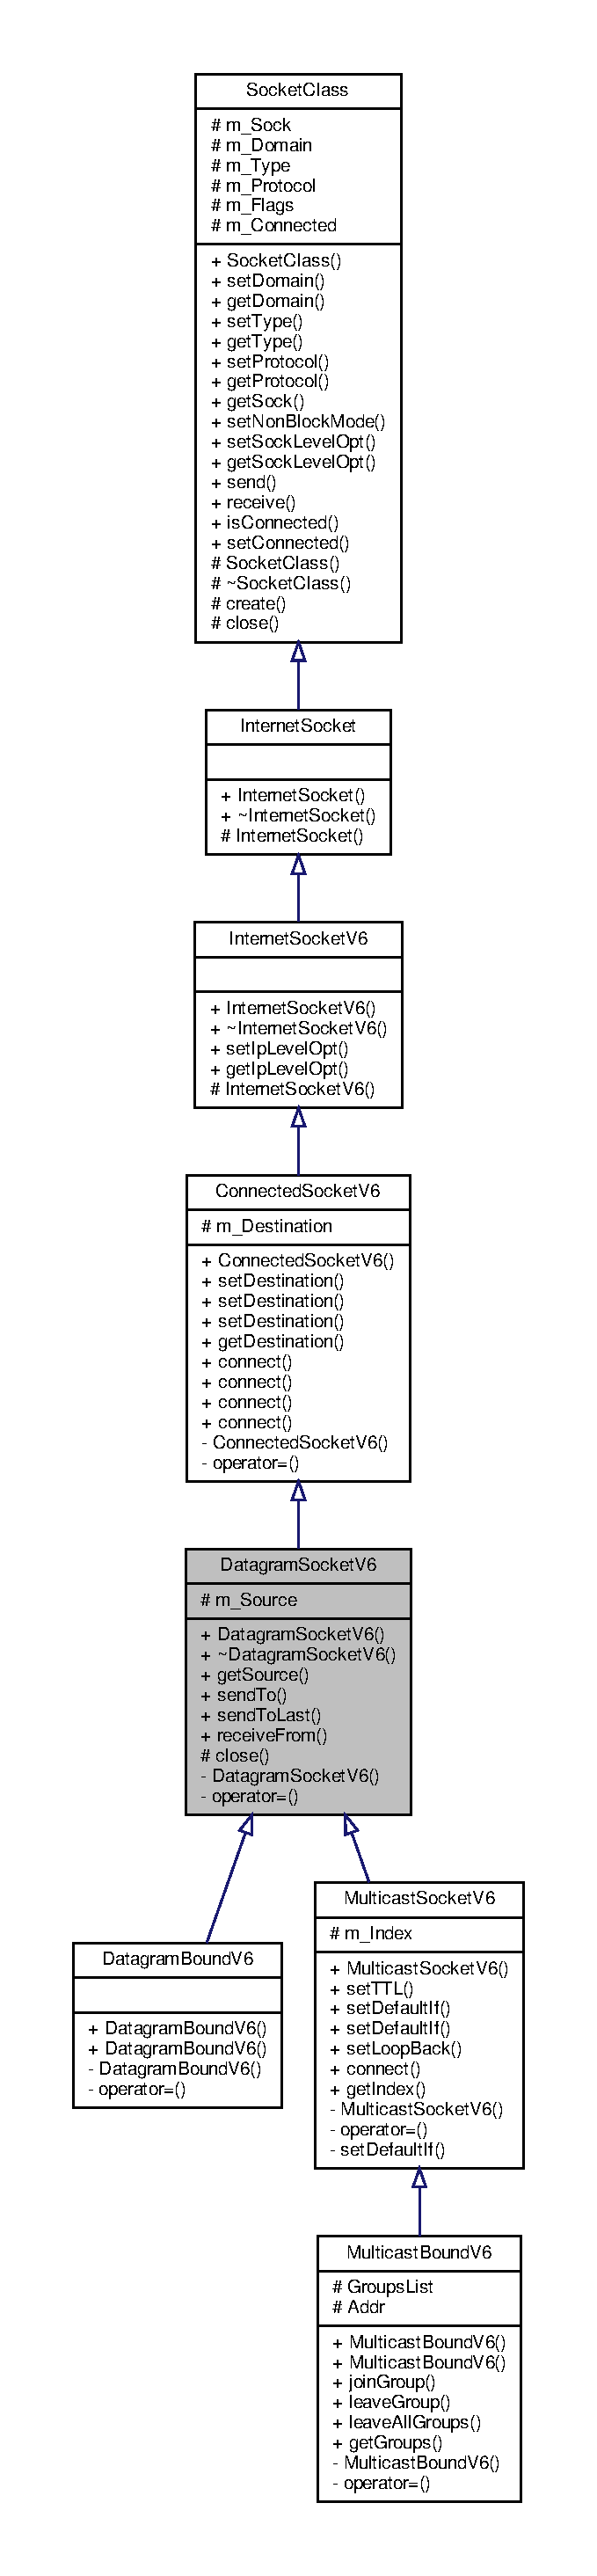
\includegraphics[height=550pt]{classDatagramSocketV6__inherit__graph}
\end{center}
\end{figure}
\subsection*{Public Member Functions}
\begin{DoxyCompactItemize}
\item 
\hyperlink{classDatagramSocketV6_a6ef4a140f2eca611448413ef768ffee3}{Datagram\+Socket\+V6} (int protocol=0)
\item 
virtual \hyperlink{classDatagramSocketV6_a4057e9a144bcc237411d32f76d034b7c}{$\sim$\+Datagram\+Socket\+V6} ()
\begin{DoxyCompactList}\small\item\em Destructor. \end{DoxyCompactList}\item 
sockaddr\+\_\+in6 \& \hyperlink{classDatagramSocketV6_abc2e68bf8b201e882f7ef4c273f02e19}{get\+Source} ()
\item 
int \hyperlink{classDatagramSocketV6_a2dbde712807a402b1cc06aa9093932c3}{send\+To} (const void $\ast$Buffer, size\+\_\+t Length, int Flags=0)
\item 
int \hyperlink{classDatagramSocketV6_ab94e99d82f82e9819e529873aadfa567}{send\+To\+Last} (const void $\ast$Buffer, size\+\_\+t Length, int Flags=0)
\item 
int \hyperlink{classDatagramSocketV6_a86966965f492e9b7f1beb627ca7c4d4b}{receive\+From} (void $\ast$Buffer, size\+\_\+t Length, int Flags=0)
\end{DoxyCompactItemize}
\subsection*{Protected Member Functions}
\begin{DoxyCompactItemize}
\item 
virtual void \hyperlink{classDatagramSocketV6_ad002933c38f60f789a5a425921d9ca4d}{close} ()
\begin{DoxyCompactList}\small\item\em Close socket. \end{DoxyCompactList}\end{DoxyCompactItemize}
\subsection*{Protected Attributes}
\begin{DoxyCompactItemize}
\item 
sockaddr\+\_\+in6 \hyperlink{classDatagramSocketV6_a5a82b5500e449bcd0017284e8b18a9a5}{m\+\_\+\+Source}
\begin{DoxyCompactList}\small\item\em Properties of the endpoint, that last received datagram was send from. \end{DoxyCompactList}\end{DoxyCompactItemize}
\subsection*{Private Member Functions}
\begin{DoxyCompactItemize}
\item 
\hyperlink{classDatagramSocketV6_abafce8dec242d3f9899ddcc5dfa11761}{Datagram\+Socket\+V6} (\hyperlink{classDatagramSocketV6}{Datagram\+Socket\+V6} \&d)
\item 
\hyperlink{classDatagramSocketV6}{Datagram\+Socket\+V6} \& \hyperlink{classDatagramSocketV6_a0c09ba2187bbbf0fceeba81d96d111b7}{operator=} (\hyperlink{classDatagramSocketV6}{Datagram\+Socket\+V6} \&d)
\end{DoxyCompactItemize}
\subsection*{Additional Inherited Members}


\subsection{Detailed Description}
Class for U\+DP sockets I\+Pv6. 

\subsection{Constructor \& Destructor Documentation}
\mbox{\Hypertarget{classDatagramSocketV6_a6ef4a140f2eca611448413ef768ffee3}\label{classDatagramSocketV6_a6ef4a140f2eca611448413ef768ffee3}} 
\index{Datagram\+Socket\+V6@{Datagram\+Socket\+V6}!Datagram\+Socket\+V6@{Datagram\+Socket\+V6}}
\index{Datagram\+Socket\+V6@{Datagram\+Socket\+V6}!Datagram\+Socket\+V6@{Datagram\+Socket\+V6}}
\subsubsection{\texorpdfstring{Datagram\+Socket\+V6()}{DatagramSocketV6()}\hspace{0.1cm}{\footnotesize\ttfamily [1/2]}}
{\footnotesize\ttfamily Datagram\+Socket\+V6\+::\+Datagram\+Socket\+V6 (\begin{DoxyParamCaption}\item[{int}]{protocol = {\ttfamily 0} }\end{DoxyParamCaption})}

Constructor. Default constructor. 
\begin{DoxyParams}{Parameters}
{\em protocol} & \+: socket protocol, default value -\/ 0. \\
\hline
\end{DoxyParams}

\begin{DoxyExceptions}{Exceptions}
{\em \hyperlink{classSockException}{Sock\+Exception}} & \\
\hline
\end{DoxyExceptions}
\mbox{\Hypertarget{classDatagramSocketV6_a4057e9a144bcc237411d32f76d034b7c}\label{classDatagramSocketV6_a4057e9a144bcc237411d32f76d034b7c}} 
\index{Datagram\+Socket\+V6@{Datagram\+Socket\+V6}!````~Datagram\+Socket\+V6@{$\sim$\+Datagram\+Socket\+V6}}
\index{````~Datagram\+Socket\+V6@{$\sim$\+Datagram\+Socket\+V6}!Datagram\+Socket\+V6@{Datagram\+Socket\+V6}}
\subsubsection{\texorpdfstring{$\sim$\+Datagram\+Socket\+V6()}{~DatagramSocketV6()}}
{\footnotesize\ttfamily virtual Datagram\+Socket\+V6\+::$\sim$\+Datagram\+Socket\+V6 (\begin{DoxyParamCaption}{ }\end{DoxyParamCaption})\hspace{0.3cm}{\ttfamily [inline]}, {\ttfamily [virtual]}}



Destructor. 

\mbox{\Hypertarget{classDatagramSocketV6_abafce8dec242d3f9899ddcc5dfa11761}\label{classDatagramSocketV6_abafce8dec242d3f9899ddcc5dfa11761}} 
\index{Datagram\+Socket\+V6@{Datagram\+Socket\+V6}!Datagram\+Socket\+V6@{Datagram\+Socket\+V6}}
\index{Datagram\+Socket\+V6@{Datagram\+Socket\+V6}!Datagram\+Socket\+V6@{Datagram\+Socket\+V6}}
\subsubsection{\texorpdfstring{Datagram\+Socket\+V6()}{DatagramSocketV6()}\hspace{0.1cm}{\footnotesize\ttfamily [2/2]}}
{\footnotesize\ttfamily Datagram\+Socket\+V6\+::\+Datagram\+Socket\+V6 (\begin{DoxyParamCaption}\item[{\hyperlink{classDatagramSocketV6}{Datagram\+Socket\+V6} \&}]{d }\end{DoxyParamCaption})\hspace{0.3cm}{\ttfamily [private]}}

Copy constructor. Makes the class uncopyable. 

\subsection{Member Function Documentation}
\mbox{\Hypertarget{classDatagramSocketV6_ad002933c38f60f789a5a425921d9ca4d}\label{classDatagramSocketV6_ad002933c38f60f789a5a425921d9ca4d}} 
\index{Datagram\+Socket\+V6@{Datagram\+Socket\+V6}!close@{close}}
\index{close@{close}!Datagram\+Socket\+V6@{Datagram\+Socket\+V6}}
\subsubsection{\texorpdfstring{close()}{close()}}
{\footnotesize\ttfamily virtual void Datagram\+Socket\+V6\+::close (\begin{DoxyParamCaption}{ }\end{DoxyParamCaption})\hspace{0.3cm}{\ttfamily [inline]}, {\ttfamily [protected]}, {\ttfamily [virtual]}}



Close socket. 



Implements \hyperlink{classSocketClass_a92c8c1b22b98f0231932cbd84cdc4cfe}{Socket\+Class}.

\mbox{\Hypertarget{classDatagramSocketV6_abc2e68bf8b201e882f7ef4c273f02e19}\label{classDatagramSocketV6_abc2e68bf8b201e882f7ef4c273f02e19}} 
\index{Datagram\+Socket\+V6@{Datagram\+Socket\+V6}!get\+Source@{get\+Source}}
\index{get\+Source@{get\+Source}!Datagram\+Socket\+V6@{Datagram\+Socket\+V6}}
\subsubsection{\texorpdfstring{get\+Source()}{getSource()}}
{\footnotesize\ttfamily sockaddr\+\_\+in6\& Datagram\+Socket\+V6\+::get\+Source (\begin{DoxyParamCaption}{ }\end{DoxyParamCaption})\hspace{0.3cm}{\ttfamily [inline]}}

Delivers source of the last received datagram. \begin{DoxyReturn}{Returns}
sockaddr\+\_\+in6 structure field with source of the last received datagram. 
\end{DoxyReturn}
\mbox{\Hypertarget{classDatagramSocketV6_a0c09ba2187bbbf0fceeba81d96d111b7}\label{classDatagramSocketV6_a0c09ba2187bbbf0fceeba81d96d111b7}} 
\index{Datagram\+Socket\+V6@{Datagram\+Socket\+V6}!operator=@{operator=}}
\index{operator=@{operator=}!Datagram\+Socket\+V6@{Datagram\+Socket\+V6}}
\subsubsection{\texorpdfstring{operator=()}{operator=()}}
{\footnotesize\ttfamily \hyperlink{classDatagramSocketV6}{Datagram\+Socket\+V6}\& Datagram\+Socket\+V6\+::operator= (\begin{DoxyParamCaption}\item[{\hyperlink{classDatagramSocketV6}{Datagram\+Socket\+V6} \&}]{d }\end{DoxyParamCaption})\hspace{0.3cm}{\ttfamily [private]}}

Operator assign. Makes the class uncopyable. \mbox{\Hypertarget{classDatagramSocketV6_a86966965f492e9b7f1beb627ca7c4d4b}\label{classDatagramSocketV6_a86966965f492e9b7f1beb627ca7c4d4b}} 
\index{Datagram\+Socket\+V6@{Datagram\+Socket\+V6}!receive\+From@{receive\+From}}
\index{receive\+From@{receive\+From}!Datagram\+Socket\+V6@{Datagram\+Socket\+V6}}
\subsubsection{\texorpdfstring{receive\+From()}{receiveFrom()}}
{\footnotesize\ttfamily int Datagram\+Socket\+V6\+::receive\+From (\begin{DoxyParamCaption}\item[{void $\ast$}]{Buffer,  }\item[{size\+\_\+t}]{Length,  }\item[{int}]{Flags = {\ttfamily 0} }\end{DoxyParamCaption})}

Receive datagram. 
\begin{DoxyParams}{Parameters}
{\em Buffer} & \+: buffer for received data . \\
\hline
{\em Length} & \+: size of buffer. \\
\hline
{\em Flags} & \+: flags, default value -\/ 0. \\
\hline
\end{DoxyParams}

\begin{DoxyExceptions}{Exceptions}
{\em \hyperlink{classSockException}{Sock\+Exception}} & \\
\hline
\end{DoxyExceptions}
\mbox{\Hypertarget{classDatagramSocketV6_a2dbde712807a402b1cc06aa9093932c3}\label{classDatagramSocketV6_a2dbde712807a402b1cc06aa9093932c3}} 
\index{Datagram\+Socket\+V6@{Datagram\+Socket\+V6}!send\+To@{send\+To}}
\index{send\+To@{send\+To}!Datagram\+Socket\+V6@{Datagram\+Socket\+V6}}
\subsubsection{\texorpdfstring{send\+To()}{sendTo()}}
{\footnotesize\ttfamily int Datagram\+Socket\+V6\+::send\+To (\begin{DoxyParamCaption}\item[{const void $\ast$}]{Buffer,  }\item[{size\+\_\+t}]{Length,  }\item[{int}]{Flags = {\ttfamily 0} }\end{DoxyParamCaption})}

Send datagram to defined destination. Destination should be define with \char`\"{}set\+Destination\char`\"{} method. 
\begin{DoxyParams}{Parameters}
{\em Buffer} & \+: data for send. \\
\hline
{\em Length} & \+: size of data to send. \\
\hline
{\em Flags} & \+: flags, default value -\/ 0. \\
\hline
\end{DoxyParams}

\begin{DoxyExceptions}{Exceptions}
{\em \hyperlink{classSockException}{Sock\+Exception}} & \\
\hline
\end{DoxyExceptions}
\mbox{\Hypertarget{classDatagramSocketV6_ab94e99d82f82e9819e529873aadfa567}\label{classDatagramSocketV6_ab94e99d82f82e9819e529873aadfa567}} 
\index{Datagram\+Socket\+V6@{Datagram\+Socket\+V6}!send\+To\+Last@{send\+To\+Last}}
\index{send\+To\+Last@{send\+To\+Last}!Datagram\+Socket\+V6@{Datagram\+Socket\+V6}}
\subsubsection{\texorpdfstring{send\+To\+Last()}{sendToLast()}}
{\footnotesize\ttfamily int Datagram\+Socket\+V6\+::send\+To\+Last (\begin{DoxyParamCaption}\item[{const void $\ast$}]{Buffer,  }\item[{size\+\_\+t}]{Length,  }\item[{int}]{Flags = {\ttfamily 0} }\end{DoxyParamCaption})\hspace{0.3cm}{\ttfamily [inline]}}

Send datagram to the source of last received datagram. 
\begin{DoxyParams}{Parameters}
{\em Buffer} & \+: data for send. \\
\hline
{\em Length} & \+: size of data to send. \\
\hline
{\em Flags} & \+: flags, default value -\/ 0. \\
\hline
\end{DoxyParams}

\begin{DoxyExceptions}{Exceptions}
{\em \hyperlink{classSockException}{Sock\+Exception}} & \\
\hline
\end{DoxyExceptions}


\subsection{Member Data Documentation}
\mbox{\Hypertarget{classDatagramSocketV6_a5a82b5500e449bcd0017284e8b18a9a5}\label{classDatagramSocketV6_a5a82b5500e449bcd0017284e8b18a9a5}} 
\index{Datagram\+Socket\+V6@{Datagram\+Socket\+V6}!m\+\_\+\+Source@{m\+\_\+\+Source}}
\index{m\+\_\+\+Source@{m\+\_\+\+Source}!Datagram\+Socket\+V6@{Datagram\+Socket\+V6}}
\subsubsection{\texorpdfstring{m\+\_\+\+Source}{m\_Source}}
{\footnotesize\ttfamily sockaddr\+\_\+in6 Datagram\+Socket\+V6\+::m\+\_\+\+Source\hspace{0.3cm}{\ttfamily [protected]}}



Properties of the endpoint, that last received datagram was send from. 



The documentation for this class was generated from the following files\+:\begin{DoxyCompactItemize}
\item 
\hyperlink{DatagramSocketV6_8h}{Datagram\+Socket\+V6.\+h}\item 
\hyperlink{DatagramSocketV6_8cpp}{Datagram\+Socket\+V6.\+cpp}\end{DoxyCompactItemize}

\hypertarget{classDisconnectException}{}\section{Disconnect\+Exception Class Reference}
\label{classDisconnectException}\index{Disconnect\+Exception@{Disconnect\+Exception}}


{\ttfamily \#include $<$Disconnect\+Exception.\+h$>$}



Inheritance diagram for Disconnect\+Exception\+:\nopagebreak
\begin{figure}[H]
\begin{center}
\leavevmode
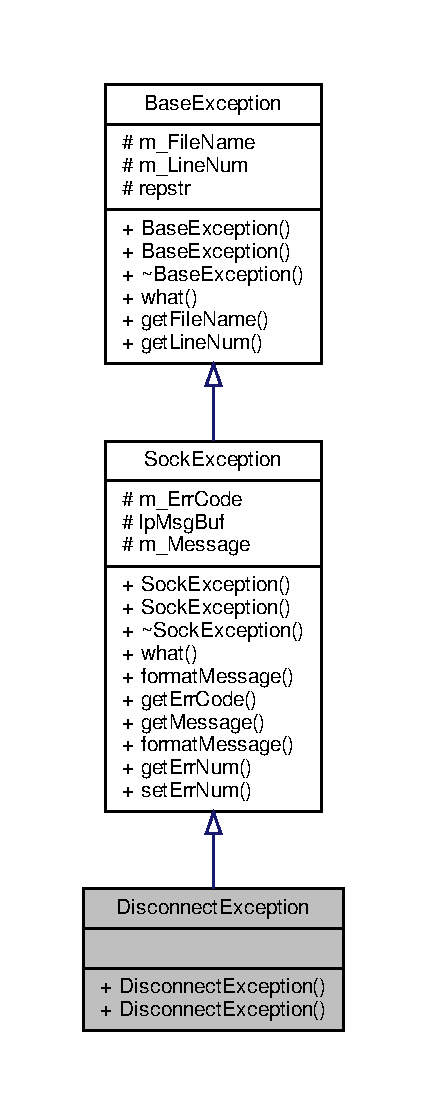
\includegraphics[width=205pt]{classDisconnectException__inherit__graph}
\end{center}
\end{figure}
\subsection*{Public Member Functions}
\begin{DoxyCompactItemize}
\item 
\hyperlink{classDisconnectException_a83047c402b0a683f0d9ca5a424775510}{Disconnect\+Exception} (const char $\ast$File\+Name, int Line\+Num, int errcode=\hyperlink{sockclasslib_8h_a990acc876290fc28437b4cce88c897a8}{W\+S\+A\+E\+C\+O\+N\+N\+R\+E\+S\+ET})
\item 
\hyperlink{classDisconnectException_af47f56084a2c38ed629b4e0ea486a3dd}{Disconnect\+Exception} (const char $\ast$File\+Name, int Line\+Num, const char $\ast$Msg)
\end{DoxyCompactItemize}
\subsection*{Additional Inherited Members}


\subsection{Detailed Description}
Stream socket disconnection exception. 

\subsection{Constructor \& Destructor Documentation}
\mbox{\Hypertarget{classDisconnectException_a83047c402b0a683f0d9ca5a424775510}\label{classDisconnectException_a83047c402b0a683f0d9ca5a424775510}} 
\index{Disconnect\+Exception@{Disconnect\+Exception}!Disconnect\+Exception@{Disconnect\+Exception}}
\index{Disconnect\+Exception@{Disconnect\+Exception}!Disconnect\+Exception@{Disconnect\+Exception}}
\subsubsection{\texorpdfstring{Disconnect\+Exception()}{DisconnectException()}\hspace{0.1cm}{\footnotesize\ttfamily [1/2]}}
{\footnotesize\ttfamily Disconnect\+Exception\+::\+Disconnect\+Exception (\begin{DoxyParamCaption}\item[{const char $\ast$}]{File\+Name,  }\item[{int}]{Line\+Num,  }\item[{int}]{errcode = {\ttfamily \hyperlink{sockclasslib_8h_a990acc876290fc28437b4cce88c897a8}{W\+S\+A\+E\+C\+O\+N\+N\+R\+E\+S\+ET}} }\end{DoxyParamCaption})\hspace{0.3cm}{\ttfamily [inline]}}

Constructor

Constructs exception object with filename and line number. 
\begin{DoxyParams}{Parameters}
{\em File\+Name} & \+: name of source file. \\
\hline
{\em Line\+Num} & \+: number of code line. \\
\hline
{\em errcode} & \+: error numeric code, default value C\+O\+N\+N\+R\+E\+S\+ET. \\
\hline
\end{DoxyParams}
\mbox{\Hypertarget{classDisconnectException_af47f56084a2c38ed629b4e0ea486a3dd}\label{classDisconnectException_af47f56084a2c38ed629b4e0ea486a3dd}} 
\index{Disconnect\+Exception@{Disconnect\+Exception}!Disconnect\+Exception@{Disconnect\+Exception}}
\index{Disconnect\+Exception@{Disconnect\+Exception}!Disconnect\+Exception@{Disconnect\+Exception}}
\subsubsection{\texorpdfstring{Disconnect\+Exception()}{DisconnectException()}\hspace{0.1cm}{\footnotesize\ttfamily [2/2]}}
{\footnotesize\ttfamily Disconnect\+Exception\+::\+Disconnect\+Exception (\begin{DoxyParamCaption}\item[{const char $\ast$}]{File\+Name,  }\item[{int}]{Line\+Num,  }\item[{const char $\ast$}]{Msg }\end{DoxyParamCaption})\hspace{0.3cm}{\ttfamily [inline]}}

Constructor

Constructs exception object with filename, line number and text message 
\begin{DoxyParams}{Parameters}
{\em File\+Name} & \+: name of source file. \\
\hline
{\em Line\+Num} & \+: number of code line. \\
\hline
{\em Msg} & \+: user message. \\
\hline
\end{DoxyParams}


The documentation for this class was generated from the following file\+:\begin{DoxyCompactItemize}
\item 
\hyperlink{DisconnectException_8h}{Disconnect\+Exception.\+h}\end{DoxyCompactItemize}

\hypertarget{classInternetSocket}{}\section{Internet\+Socket Class Reference}
\label{classInternetSocket}\index{Internet\+Socket@{Internet\+Socket}}


{\ttfamily \#include $<$Internet\+Socket.\+h$>$}



Inheritance diagram for Internet\+Socket\+:\nopagebreak
\begin{figure}[H]
\begin{center}
\leavevmode
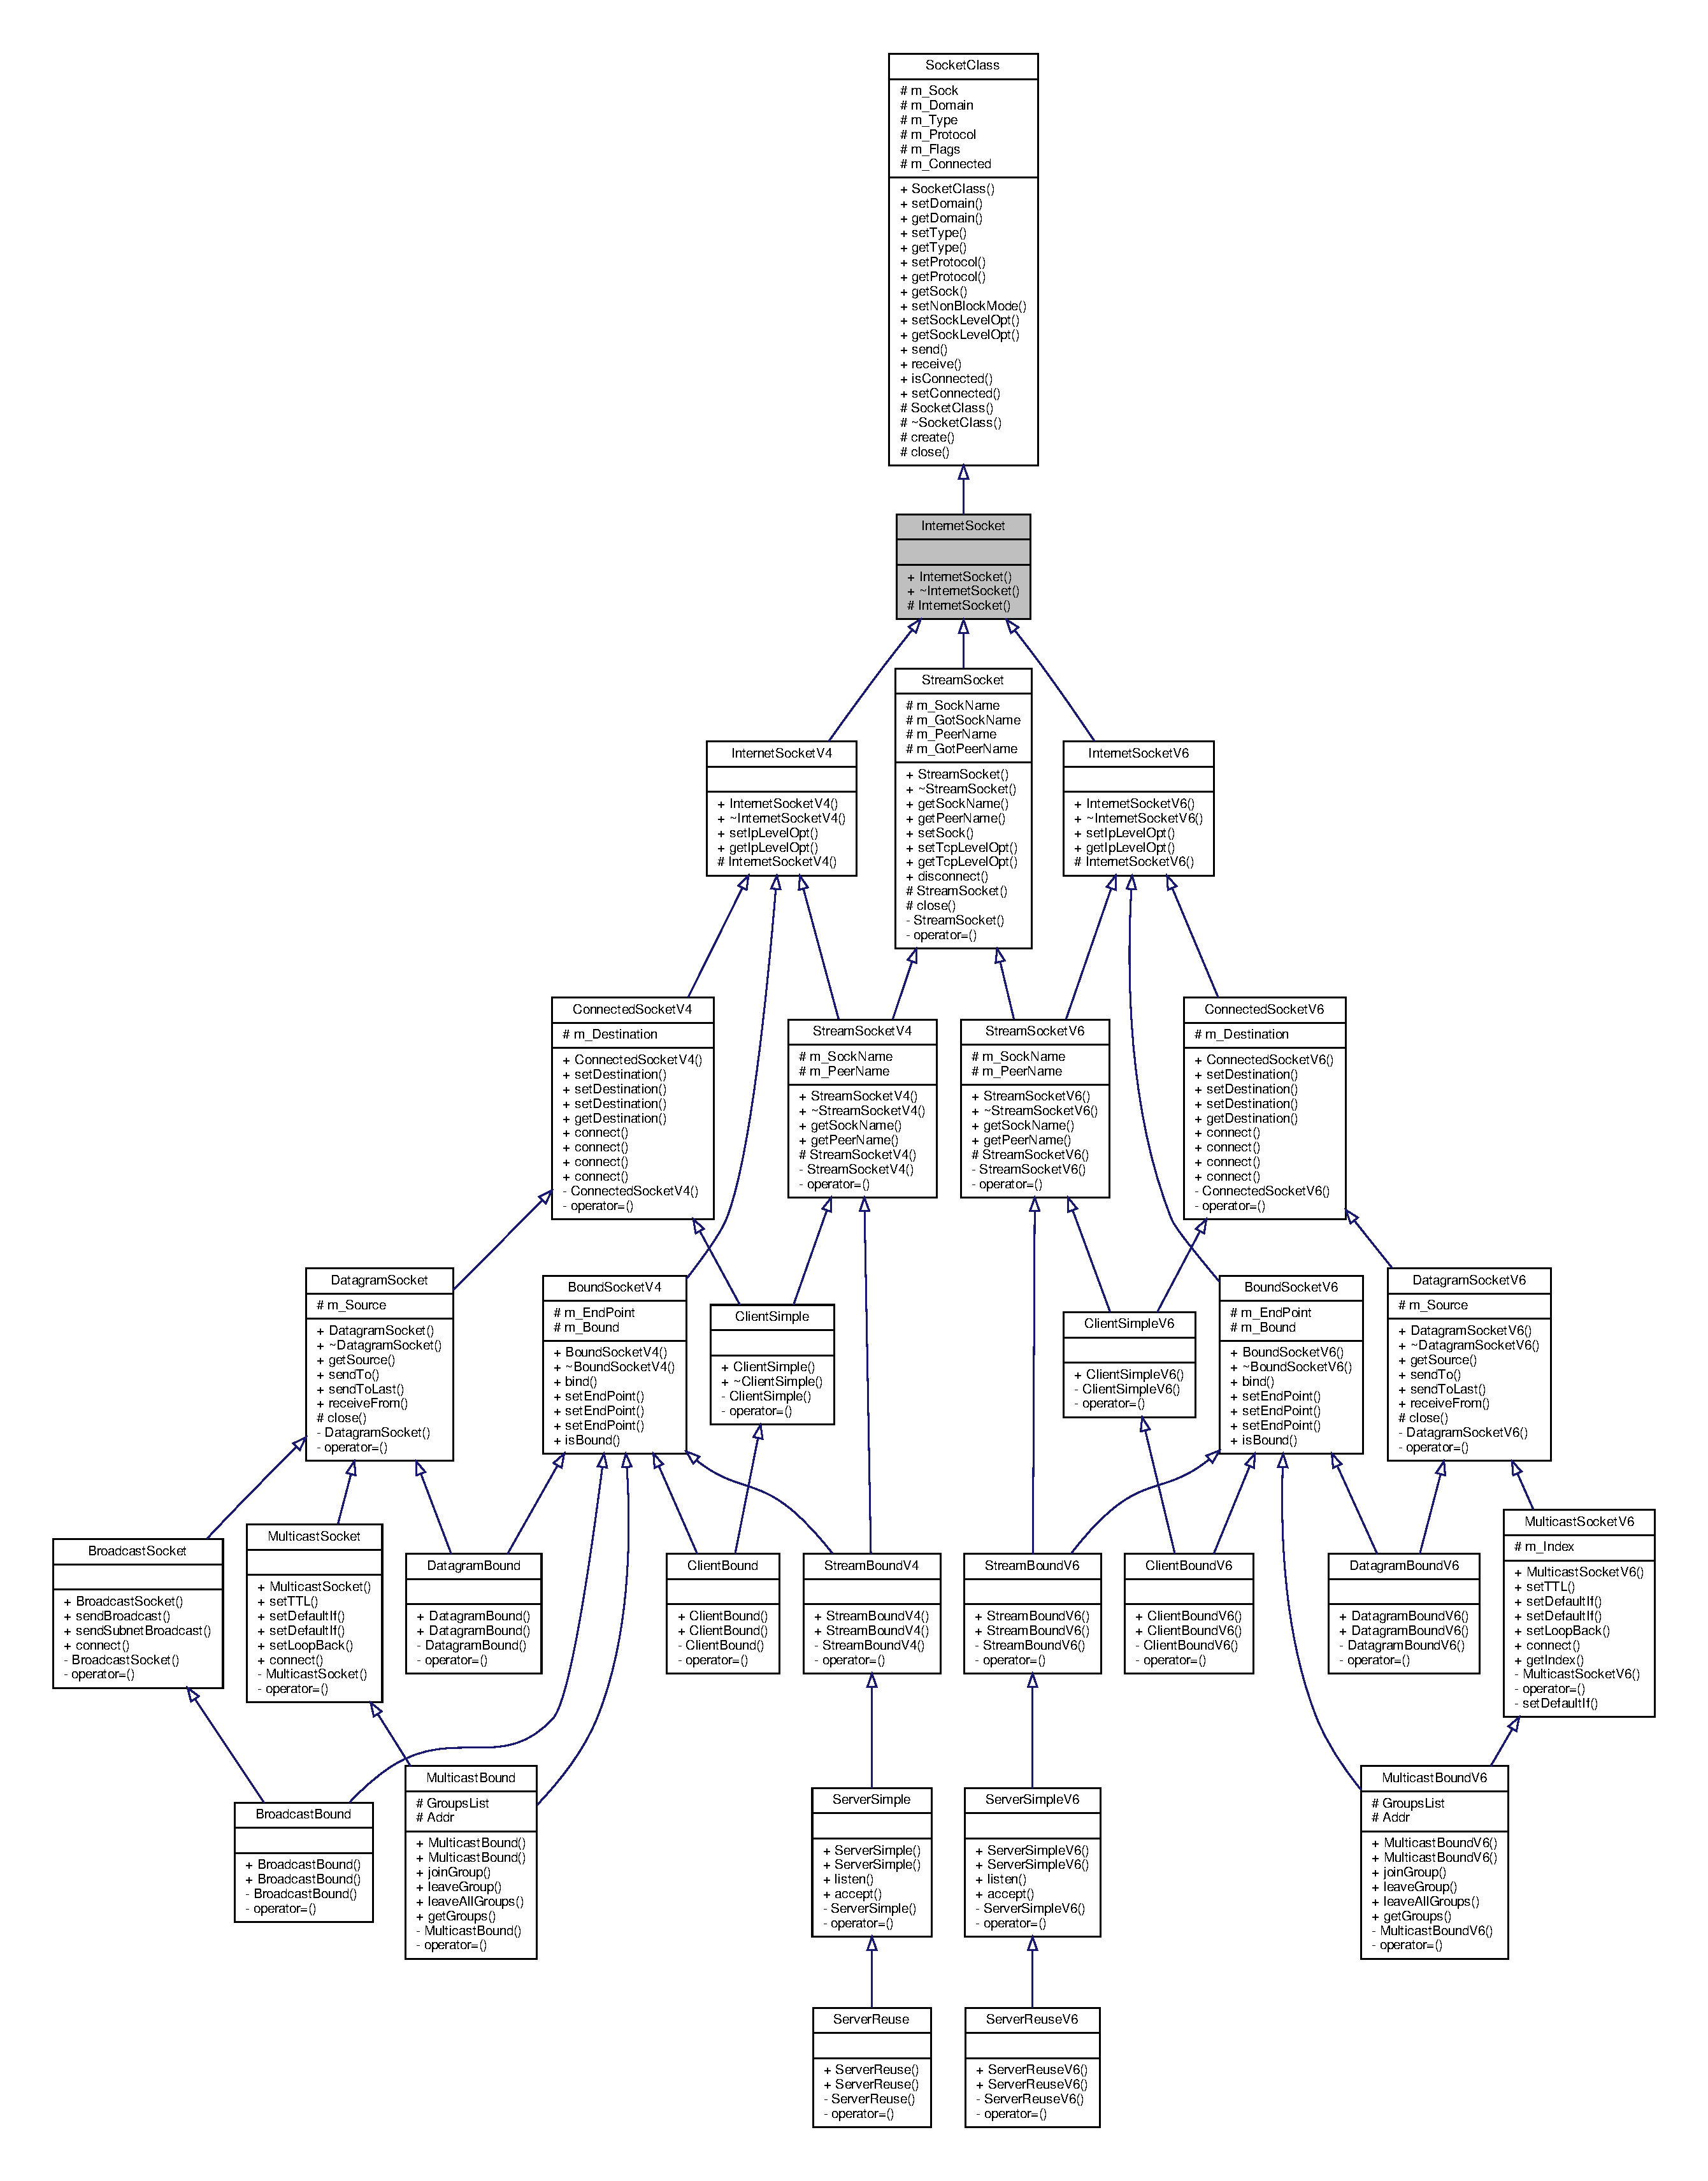
\includegraphics[width=350pt]{classInternetSocket__inherit__graph}
\end{center}
\end{figure}
\subsection*{Public Member Functions}
\begin{DoxyCompactItemize}
\item 
\hyperlink{classInternetSocket_afcbe1350ae9e2c4f256c986a371952ac}{Internet\+Socket} (\hyperlink{classSocketClass_ac940413abaa7328db8518a9f121babb6}{Sock\+Domain} domain=\hyperlink{classSocketClass_ac940413abaa7328db8518a9f121babb6aa9ec2a4d642c47813fe90f362603f1c4}{N\+O\+\_\+\+D\+O\+M\+A\+IN}, \hyperlink{classSocketClass_a2182dd9fee09459fabb99e6ae717f595}{Sock\+Type} type=\hyperlink{classSocketClass_a2182dd9fee09459fabb99e6ae717f595a8c7f955ea5b71498ff1d469345d813ad}{N\+O\+\_\+\+T\+Y\+PE}, int protocol=0)
\item 
virtual \hyperlink{classInternetSocket_aa05d862f91ae89c523f30c8af75e4bae}{$\sim$\+Internet\+Socket} ()
\begin{DoxyCompactList}\small\item\em Destructor. \end{DoxyCompactList}\end{DoxyCompactItemize}
\subsection*{Protected Member Functions}
\begin{DoxyCompactItemize}
\item 
\hyperlink{classInternetSocket_a1e7caaf50313a0f4d25ef9479c90b689}{Internet\+Socket} (int sock, \hyperlink{classSocketClass_ac940413abaa7328db8518a9f121babb6}{Sock\+Domain} domain, \hyperlink{classSocketClass_a2182dd9fee09459fabb99e6ae717f595}{Sock\+Type} type=\hyperlink{classSocketClass_a2182dd9fee09459fabb99e6ae717f595a8c7f955ea5b71498ff1d469345d813ad}{N\+O\+\_\+\+T\+Y\+PE}, int protocol=0)
\end{DoxyCompactItemize}
\subsection*{Additional Inherited Members}


\subsection{Detailed Description}
Bbase abstract class. Is base for all kinds of IP sockets, delivers functionality of manipulating IP level socket options. 

\subsection{Constructor \& Destructor Documentation}
\mbox{\Hypertarget{classInternetSocket_afcbe1350ae9e2c4f256c986a371952ac}\label{classInternetSocket_afcbe1350ae9e2c4f256c986a371952ac}} 
\index{Internet\+Socket@{Internet\+Socket}!Internet\+Socket@{Internet\+Socket}}
\index{Internet\+Socket@{Internet\+Socket}!Internet\+Socket@{Internet\+Socket}}
\subsubsection{\texorpdfstring{Internet\+Socket()}{InternetSocket()}\hspace{0.1cm}{\footnotesize\ttfamily [1/2]}}
{\footnotesize\ttfamily Internet\+Socket\+::\+Internet\+Socket (\begin{DoxyParamCaption}\item[{\hyperlink{classSocketClass_ac940413abaa7328db8518a9f121babb6}{Sock\+Domain}}]{domain = {\ttfamily \hyperlink{classSocketClass_ac940413abaa7328db8518a9f121babb6aa9ec2a4d642c47813fe90f362603f1c4}{N\+O\+\_\+\+D\+O\+M\+A\+IN}},  }\item[{\hyperlink{classSocketClass_a2182dd9fee09459fabb99e6ae717f595}{Sock\+Type}}]{type = {\ttfamily \hyperlink{classSocketClass_a2182dd9fee09459fabb99e6ae717f595a8c7f955ea5b71498ff1d469345d813ad}{N\+O\+\_\+\+T\+Y\+PE}},  }\item[{int}]{protocol = {\ttfamily 0} }\end{DoxyParamCaption})\hspace{0.3cm}{\ttfamily [inline]}}

Constructor. Default constructor. \mbox{\Hypertarget{classInternetSocket_aa05d862f91ae89c523f30c8af75e4bae}\label{classInternetSocket_aa05d862f91ae89c523f30c8af75e4bae}} 
\index{Internet\+Socket@{Internet\+Socket}!````~Internet\+Socket@{$\sim$\+Internet\+Socket}}
\index{````~Internet\+Socket@{$\sim$\+Internet\+Socket}!Internet\+Socket@{Internet\+Socket}}
\subsubsection{\texorpdfstring{$\sim$\+Internet\+Socket()}{~InternetSocket()}}
{\footnotesize\ttfamily virtual Internet\+Socket\+::$\sim$\+Internet\+Socket (\begin{DoxyParamCaption}{ }\end{DoxyParamCaption})\hspace{0.3cm}{\ttfamily [inline]}, {\ttfamily [virtual]}}



Destructor. 

\mbox{\Hypertarget{classInternetSocket_a1e7caaf50313a0f4d25ef9479c90b689}\label{classInternetSocket_a1e7caaf50313a0f4d25ef9479c90b689}} 
\index{Internet\+Socket@{Internet\+Socket}!Internet\+Socket@{Internet\+Socket}}
\index{Internet\+Socket@{Internet\+Socket}!Internet\+Socket@{Internet\+Socket}}
\subsubsection{\texorpdfstring{Internet\+Socket()}{InternetSocket()}\hspace{0.1cm}{\footnotesize\ttfamily [2/2]}}
{\footnotesize\ttfamily Internet\+Socket\+::\+Internet\+Socket (\begin{DoxyParamCaption}\item[{int}]{sock,  }\item[{\hyperlink{classSocketClass_ac940413abaa7328db8518a9f121babb6}{Sock\+Domain}}]{domain,  }\item[{\hyperlink{classSocketClass_a2182dd9fee09459fabb99e6ae717f595}{Sock\+Type}}]{type = {\ttfamily \hyperlink{classSocketClass_a2182dd9fee09459fabb99e6ae717f595a8c7f955ea5b71498ff1d469345d813ad}{N\+O\+\_\+\+T\+Y\+PE}},  }\item[{int}]{protocol = {\ttfamily 0} }\end{DoxyParamCaption})\hspace{0.3cm}{\ttfamily [inline]}, {\ttfamily [protected]}}

Constructor. Constructs socket on given socket file descriptor/handle. 
\begin{DoxyParams}{Parameters}
{\em sock} & \+: socket file descriptor/handle. \\
\hline
{\em domain} & \+: socket domain (I\+Pv4 or I\+Pv6) \\
\hline
{\em type} & \+: socket type. \\
\hline
{\em protocol} & \+: socket protocol. \\
\hline
\end{DoxyParams}


The documentation for this class was generated from the following file\+:\begin{DoxyCompactItemize}
\item 
\hyperlink{InternetSocket_8h}{Internet\+Socket.\+h}\end{DoxyCompactItemize}

\hypertarget{classInternetSocketV4}{}\section{Internet\+Socket\+V4 Class Reference}
\label{classInternetSocketV4}\index{Internet\+Socket\+V4@{Internet\+Socket\+V4}}


{\ttfamily \#include $<$Internet\+Socket\+V4.\+h$>$}



Inheritance diagram for Internet\+Socket\+V4\+:\nopagebreak
\begin{figure}[H]
\begin{center}
\leavevmode
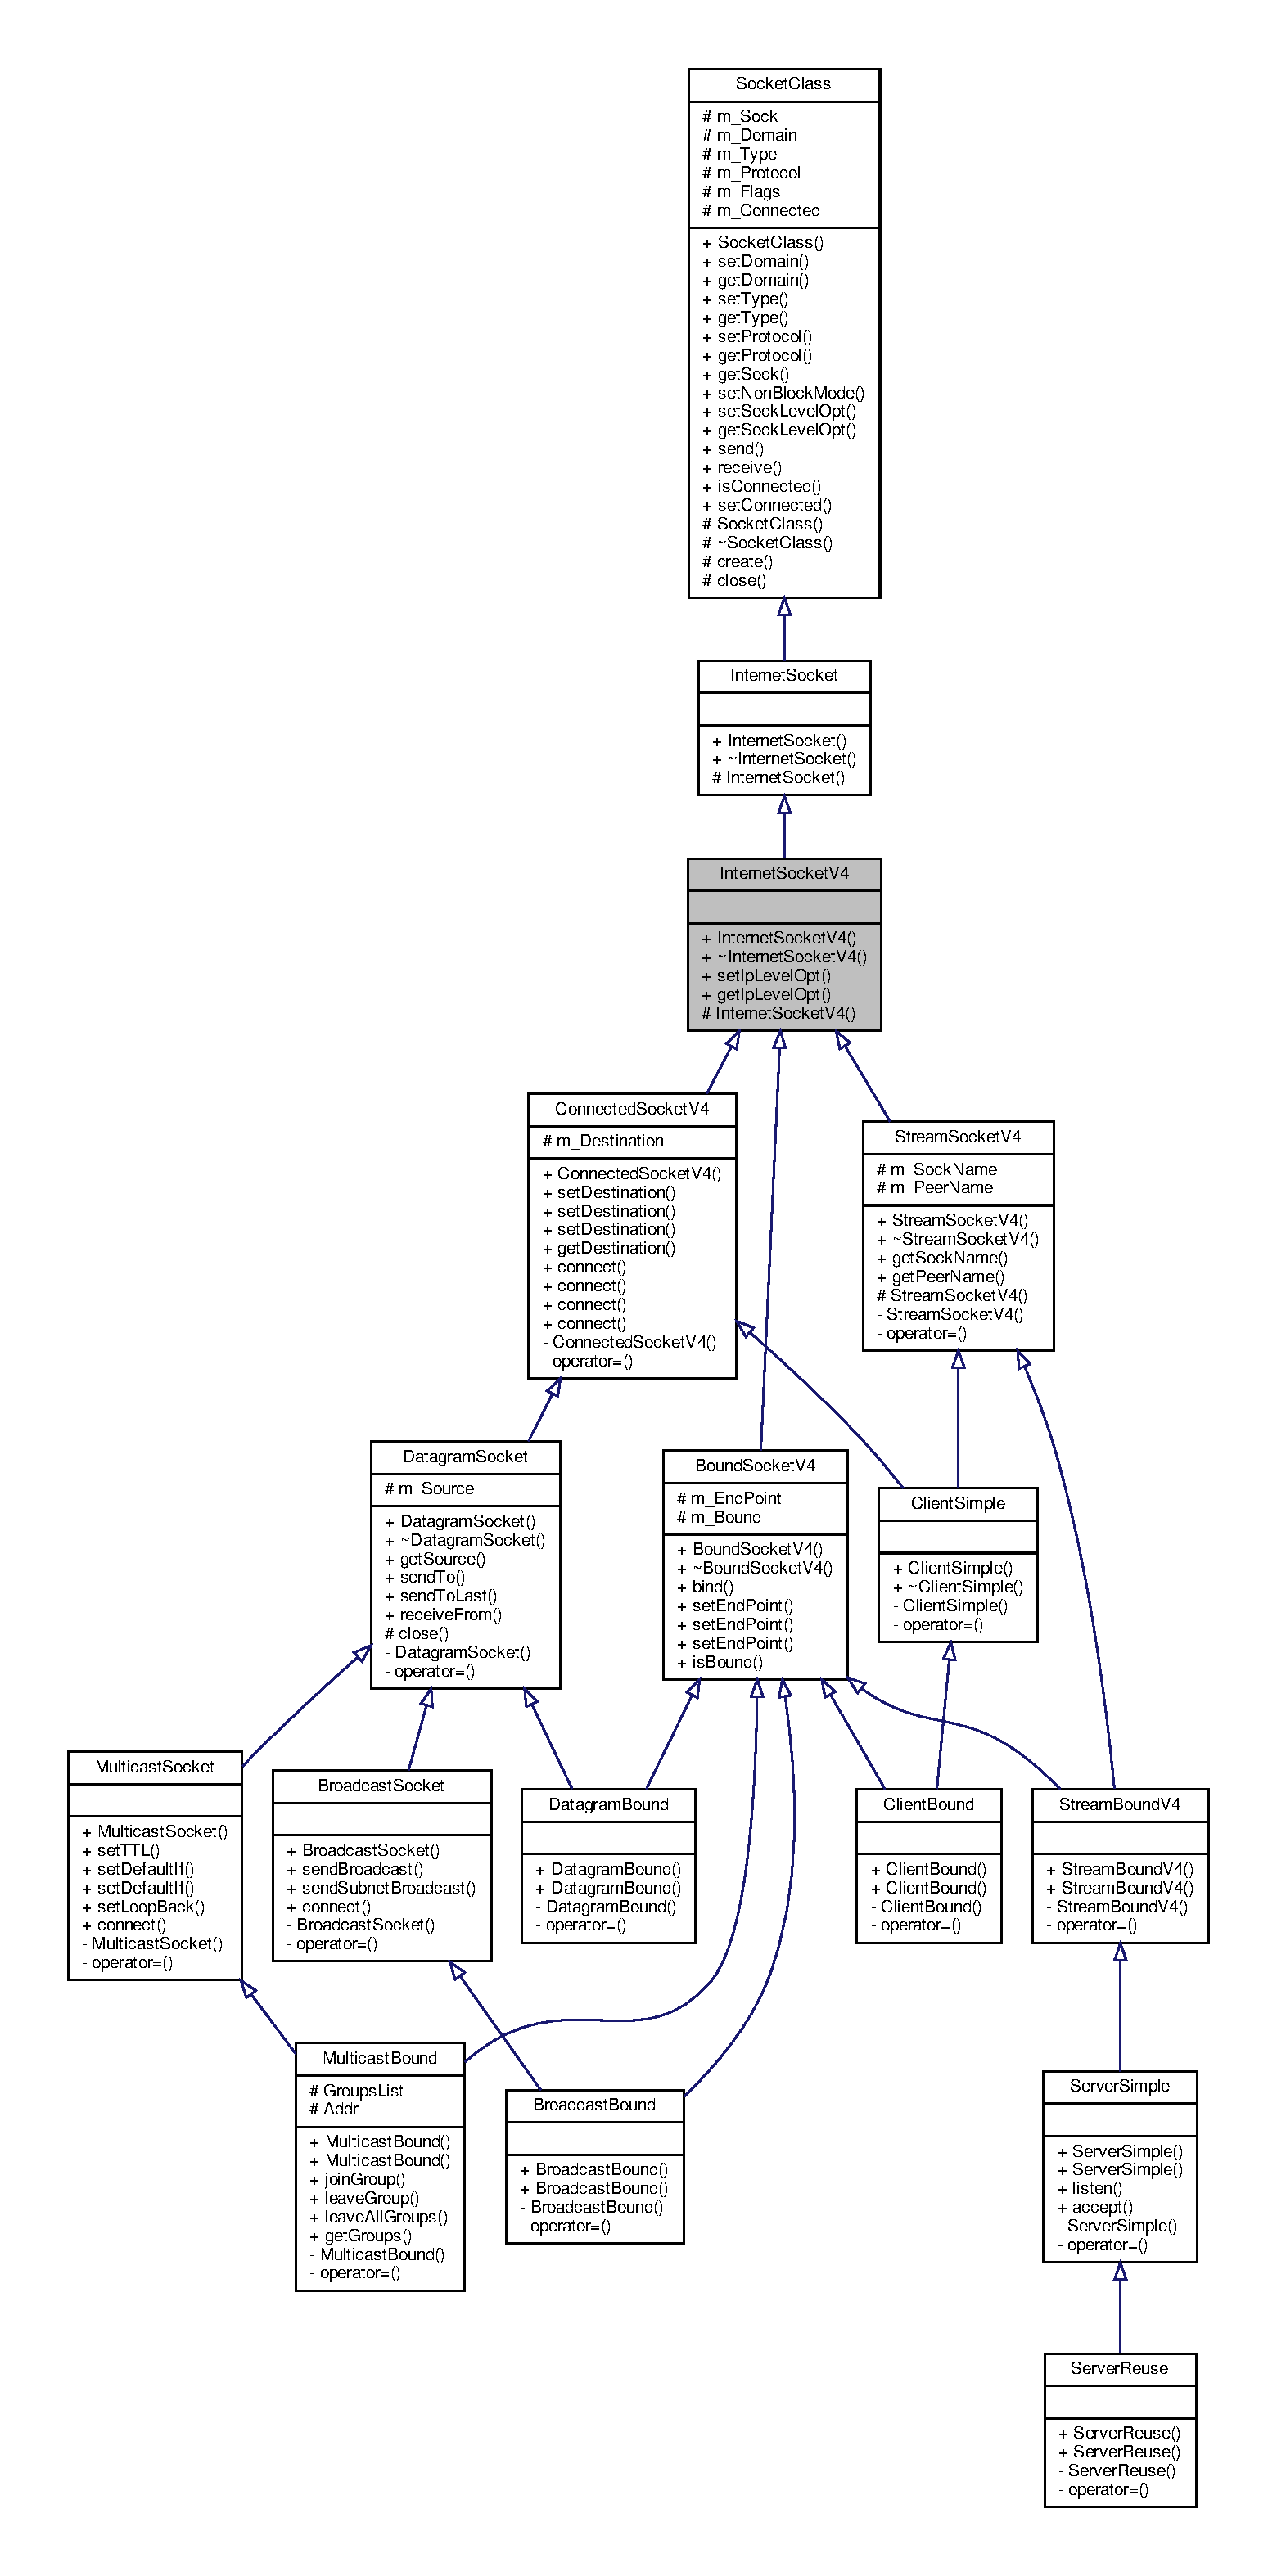
\includegraphics[height=550pt]{classInternetSocketV4__inherit__graph}
\end{center}
\end{figure}
\subsection*{Public Member Functions}
\begin{DoxyCompactItemize}
\item 
\hyperlink{classInternetSocketV4_a021a3ec93a3800a2fe879ec3df34a29b}{Internet\+Socket\+V4} (\hyperlink{classSocketClass_a2182dd9fee09459fabb99e6ae717f595}{Sock\+Type} type=\hyperlink{classSocketClass_a2182dd9fee09459fabb99e6ae717f595a8c7f955ea5b71498ff1d469345d813ad}{N\+O\+\_\+\+T\+Y\+PE}, int protocol=0)
\item 
virtual \hyperlink{classInternetSocketV4_af7edfb3b33ba40c6c93bfb9ffe0ce318}{$\sim$\+Internet\+Socket\+V4} ()
\item 
void \hyperlink{classInternetSocketV4_af890a3acb0a072f7da484113c1910a76}{set\+Ip\+Level\+Opt} (int Opt, const char $\ast$Value, int Opt\+Len)
\item 
void \hyperlink{classInternetSocketV4_a77bd7005098fb32f5214bbc140b99fe6}{get\+Ip\+Level\+Opt} (int Opt, char $\ast$Value, int $\ast$Opt\+Len)
\end{DoxyCompactItemize}
\subsection*{Protected Member Functions}
\begin{DoxyCompactItemize}
\item 
\hyperlink{classInternetSocketV4_ad2e60863f606afa5d1a45b413538baff}{Internet\+Socket\+V4} (int sock, \hyperlink{classSocketClass_a2182dd9fee09459fabb99e6ae717f595}{Sock\+Type} type=\hyperlink{classSocketClass_a2182dd9fee09459fabb99e6ae717f595a8c7f955ea5b71498ff1d469345d813ad}{N\+O\+\_\+\+T\+Y\+PE}, int protocol=0)
\end{DoxyCompactItemize}
\subsection*{Additional Inherited Members}


\subsection{Detailed Description}
I\+Pv4 base abstract class. Is base for all kinds of I\+Pv4 sockets. 

\subsection{Constructor \& Destructor Documentation}
\mbox{\Hypertarget{classInternetSocketV4_a021a3ec93a3800a2fe879ec3df34a29b}\label{classInternetSocketV4_a021a3ec93a3800a2fe879ec3df34a29b}} 
\index{Internet\+Socket\+V4@{Internet\+Socket\+V4}!Internet\+Socket\+V4@{Internet\+Socket\+V4}}
\index{Internet\+Socket\+V4@{Internet\+Socket\+V4}!Internet\+Socket\+V4@{Internet\+Socket\+V4}}
\subsubsection{\texorpdfstring{Internet\+Socket\+V4()}{InternetSocketV4()}\hspace{0.1cm}{\footnotesize\ttfamily [1/2]}}
{\footnotesize\ttfamily Internet\+Socket\+V4\+::\+Internet\+Socket\+V4 (\begin{DoxyParamCaption}\item[{\hyperlink{classSocketClass_a2182dd9fee09459fabb99e6ae717f595}{Sock\+Type}}]{type = {\ttfamily \hyperlink{classSocketClass_a2182dd9fee09459fabb99e6ae717f595a8c7f955ea5b71498ff1d469345d813ad}{N\+O\+\_\+\+T\+Y\+PE}},  }\item[{int}]{protocol = {\ttfamily 0} }\end{DoxyParamCaption})\hspace{0.3cm}{\ttfamily [inline]}}

Constructor. Default constructor. \mbox{\Hypertarget{classInternetSocketV4_af7edfb3b33ba40c6c93bfb9ffe0ce318}\label{classInternetSocketV4_af7edfb3b33ba40c6c93bfb9ffe0ce318}} 
\index{Internet\+Socket\+V4@{Internet\+Socket\+V4}!````~Internet\+Socket\+V4@{$\sim$\+Internet\+Socket\+V4}}
\index{````~Internet\+Socket\+V4@{$\sim$\+Internet\+Socket\+V4}!Internet\+Socket\+V4@{Internet\+Socket\+V4}}
\subsubsection{\texorpdfstring{$\sim$\+Internet\+Socket\+V4()}{~InternetSocketV4()}}
{\footnotesize\ttfamily virtual Internet\+Socket\+V4\+::$\sim$\+Internet\+Socket\+V4 (\begin{DoxyParamCaption}{ }\end{DoxyParamCaption})\hspace{0.3cm}{\ttfamily [inline]}, {\ttfamily [virtual]}}

\mbox{\Hypertarget{classInternetSocketV4_ad2e60863f606afa5d1a45b413538baff}\label{classInternetSocketV4_ad2e60863f606afa5d1a45b413538baff}} 
\index{Internet\+Socket\+V4@{Internet\+Socket\+V4}!Internet\+Socket\+V4@{Internet\+Socket\+V4}}
\index{Internet\+Socket\+V4@{Internet\+Socket\+V4}!Internet\+Socket\+V4@{Internet\+Socket\+V4}}
\subsubsection{\texorpdfstring{Internet\+Socket\+V4()}{InternetSocketV4()}\hspace{0.1cm}{\footnotesize\ttfamily [2/2]}}
{\footnotesize\ttfamily Internet\+Socket\+V4\+::\+Internet\+Socket\+V4 (\begin{DoxyParamCaption}\item[{int}]{sock,  }\item[{\hyperlink{classSocketClass_a2182dd9fee09459fabb99e6ae717f595}{Sock\+Type}}]{type = {\ttfamily \hyperlink{classSocketClass_a2182dd9fee09459fabb99e6ae717f595a8c7f955ea5b71498ff1d469345d813ad}{N\+O\+\_\+\+T\+Y\+PE}},  }\item[{int}]{protocol = {\ttfamily 0} }\end{DoxyParamCaption})\hspace{0.3cm}{\ttfamily [inline]}, {\ttfamily [protected]}}

Constructor. Constructs socket on given socket file descriptor/handle. 
\begin{DoxyParams}{Parameters}
{\em sock} & \+: socket file descriptor/handle. \\
\hline
{\em type} & \+: socket type. \\
\hline
{\em protocol} & \+: socket protocol. \\
\hline
\end{DoxyParams}


\subsection{Member Function Documentation}
\mbox{\Hypertarget{classInternetSocketV4_a77bd7005098fb32f5214bbc140b99fe6}\label{classInternetSocketV4_a77bd7005098fb32f5214bbc140b99fe6}} 
\index{Internet\+Socket\+V4@{Internet\+Socket\+V4}!get\+Ip\+Level\+Opt@{get\+Ip\+Level\+Opt}}
\index{get\+Ip\+Level\+Opt@{get\+Ip\+Level\+Opt}!Internet\+Socket\+V4@{Internet\+Socket\+V4}}
\subsubsection{\texorpdfstring{get\+Ip\+Level\+Opt()}{getIpLevelOpt()}}
{\footnotesize\ttfamily void Internet\+Socket\+V4\+::get\+Ip\+Level\+Opt (\begin{DoxyParamCaption}\item[{int}]{Opt,  }\item[{char $\ast$}]{Value,  }\item[{int $\ast$}]{Opt\+Len }\end{DoxyParamCaption})}

Deliver I\+Pv4 level option. 
\begin{DoxyParams}{Parameters}
{\em Opt} & \+: option type. \\
\hline
{\em Value} & \+: option value. \\
\hline
{\em Opt\+Len} & \+: option value length. \\
\hline
\end{DoxyParams}

\begin{DoxyExceptions}{Exceptions}
{\em \hyperlink{classSockException}{Sock\+Exception}} & \\
\hline
\end{DoxyExceptions}
\mbox{\Hypertarget{classInternetSocketV4_af890a3acb0a072f7da484113c1910a76}\label{classInternetSocketV4_af890a3acb0a072f7da484113c1910a76}} 
\index{Internet\+Socket\+V4@{Internet\+Socket\+V4}!set\+Ip\+Level\+Opt@{set\+Ip\+Level\+Opt}}
\index{set\+Ip\+Level\+Opt@{set\+Ip\+Level\+Opt}!Internet\+Socket\+V4@{Internet\+Socket\+V4}}
\subsubsection{\texorpdfstring{set\+Ip\+Level\+Opt()}{setIpLevelOpt()}}
{\footnotesize\ttfamily void Internet\+Socket\+V4\+::set\+Ip\+Level\+Opt (\begin{DoxyParamCaption}\item[{int}]{Opt,  }\item[{const char $\ast$}]{Value,  }\item[{int}]{Opt\+Len }\end{DoxyParamCaption})}

Set I\+Pv4 level option. 
\begin{DoxyParams}{Parameters}
{\em Opt} & \+: option type. \\
\hline
{\em Value} & \+: option value. \\
\hline
{\em Opt\+Len} & \+: option value length. \\
\hline
\end{DoxyParams}

\begin{DoxyExceptions}{Exceptions}
{\em \hyperlink{classSockException}{Sock\+Exception}} & \\
\hline
\end{DoxyExceptions}


The documentation for this class was generated from the following files\+:\begin{DoxyCompactItemize}
\item 
\hyperlink{InternetSocketV4_8h}{Internet\+Socket\+V4.\+h}\item 
\hyperlink{InternetSocketV4_8cpp}{Internet\+Socket\+V4.\+cpp}\end{DoxyCompactItemize}

\hypertarget{classInternetSocketV6}{}\section{Internet\+Socket\+V6 Class Reference}
\label{classInternetSocketV6}\index{Internet\+Socket\+V6@{Internet\+Socket\+V6}}


{\ttfamily \#include $<$Internet\+Socket\+V6.\+h$>$}



Inheritance diagram for Internet\+Socket\+V6\+:\nopagebreak
\begin{figure}[H]
\begin{center}
\leavevmode
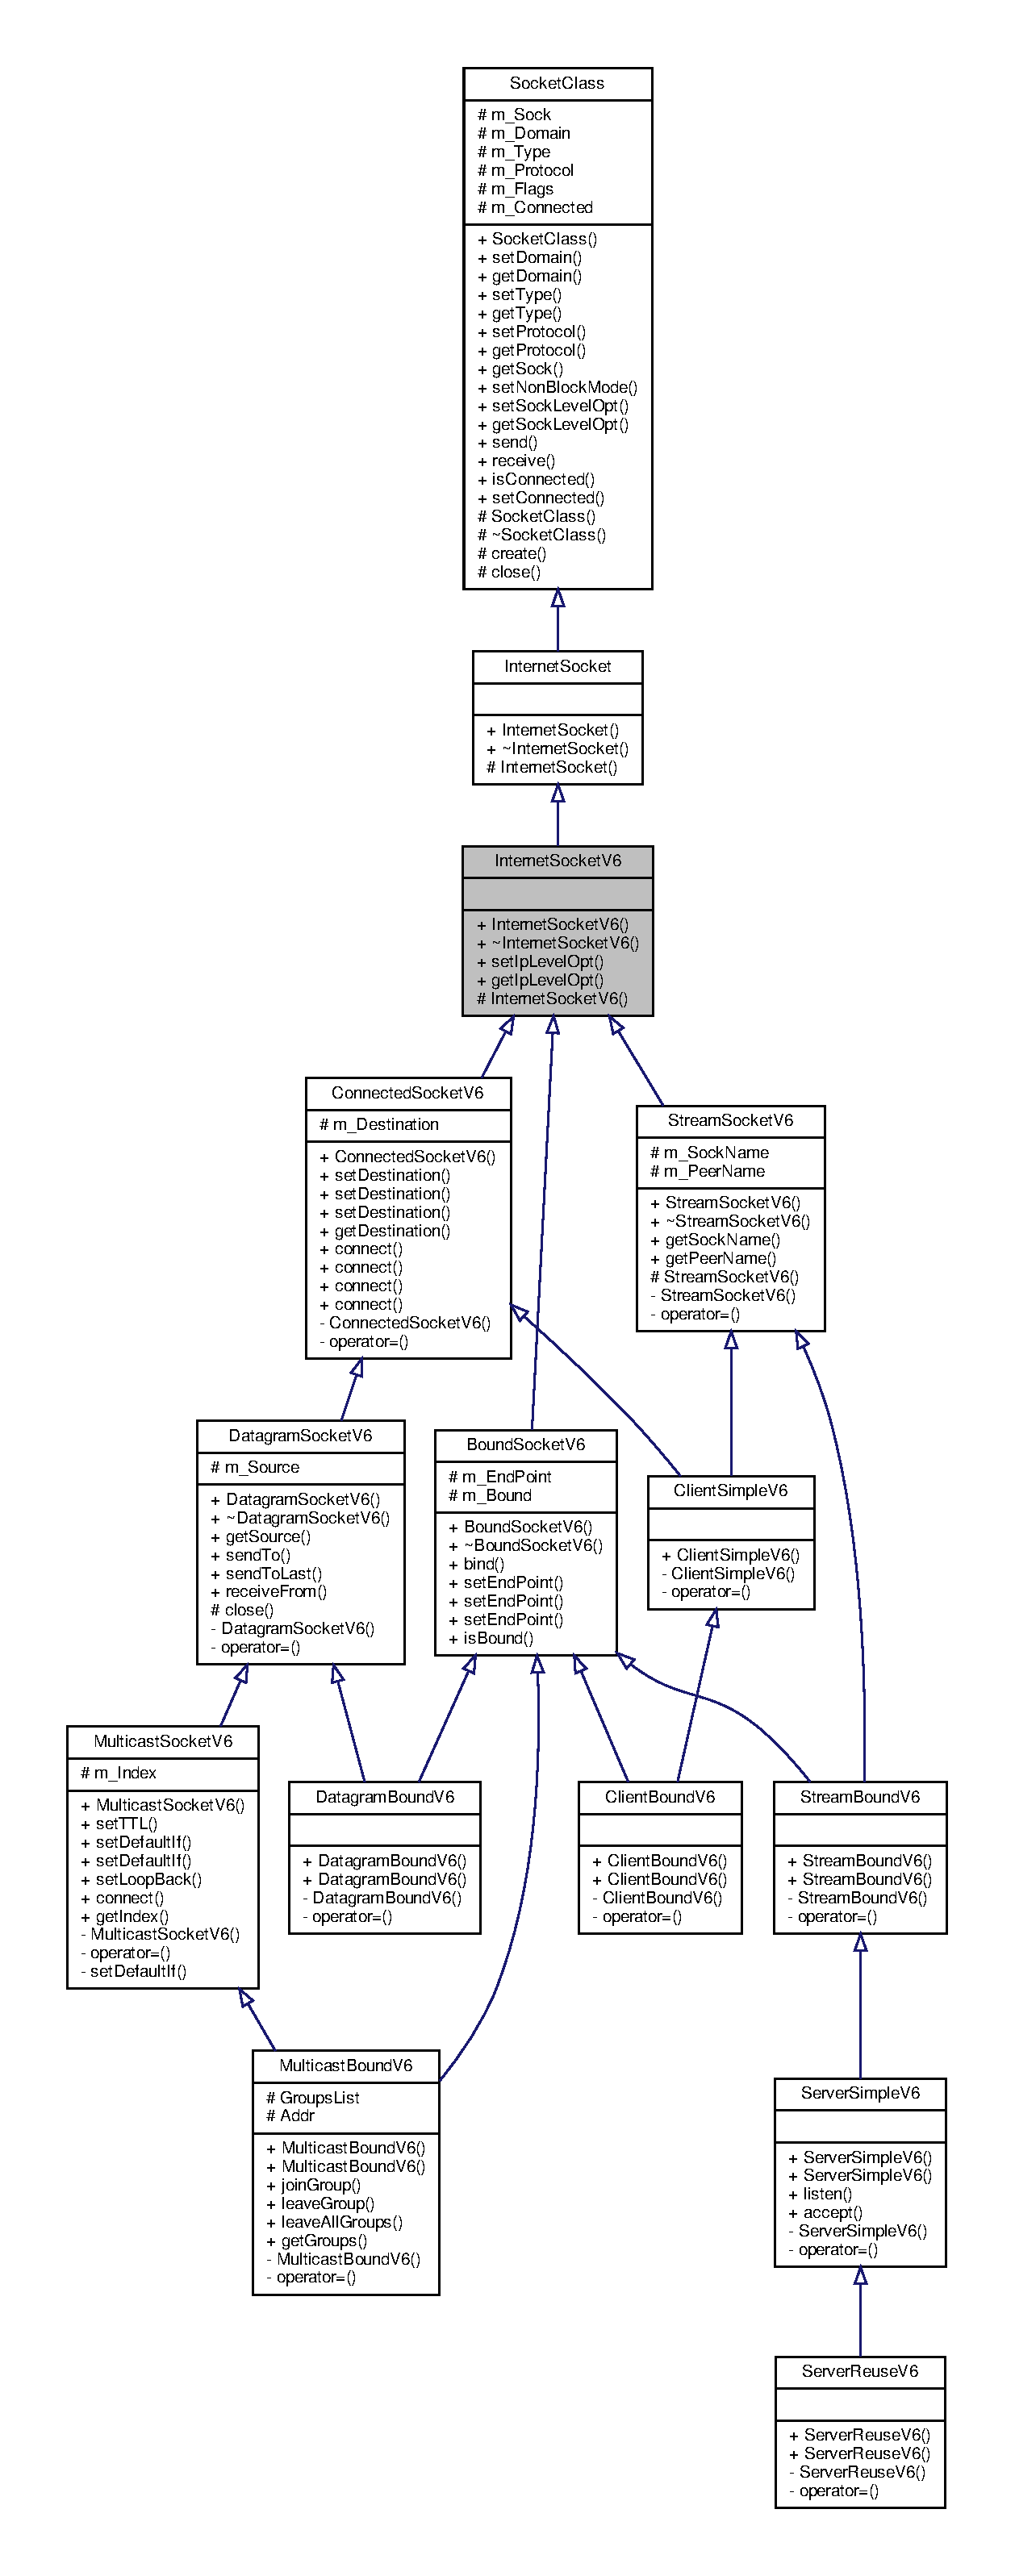
\includegraphics[height=550pt]{classInternetSocketV6__inherit__graph}
\end{center}
\end{figure}
\subsection*{Public Member Functions}
\begin{DoxyCompactItemize}
\item 
\hyperlink{classInternetSocketV6_a9be445b17d5fc20a56c95a129f4e3bfd}{Internet\+Socket\+V6} (\hyperlink{classSocketClass_a2182dd9fee09459fabb99e6ae717f595}{Sock\+Type} type=\hyperlink{classSocketClass_a2182dd9fee09459fabb99e6ae717f595a8c7f955ea5b71498ff1d469345d813ad}{N\+O\+\_\+\+T\+Y\+PE}, int protocol=0)
\item 
virtual \hyperlink{classInternetSocketV6_aa91c9ad4f01dd5c7a305cc868d46af2c}{$\sim$\+Internet\+Socket\+V6} ()
\item 
void \hyperlink{classInternetSocketV6_a6150f7fdce307a1b4dd0adf20cafbc54}{set\+Ip\+Level\+Opt} (int Opt, const char $\ast$Value, int Opt\+Len)
\item 
void \hyperlink{classInternetSocketV6_a455f355f674add52641d4713c42f8f6b}{get\+Ip\+Level\+Opt} (int Opt, char $\ast$Value, int $\ast$Opt\+Len)
\end{DoxyCompactItemize}
\subsection*{Protected Member Functions}
\begin{DoxyCompactItemize}
\item 
\hyperlink{classInternetSocketV6_a30243b27e0d83abaacd9c8c170fd684b}{Internet\+Socket\+V6} (int sock, \hyperlink{classSocketClass_a2182dd9fee09459fabb99e6ae717f595}{Sock\+Type} type=\hyperlink{classSocketClass_a2182dd9fee09459fabb99e6ae717f595a8c7f955ea5b71498ff1d469345d813ad}{N\+O\+\_\+\+T\+Y\+PE}, int protocol=0)
\end{DoxyCompactItemize}
\subsection*{Additional Inherited Members}


\subsection{Detailed Description}
I\+Pv6 base abstract class. Is base for all kinds of I\+Pv6 sockets. 

\subsection{Constructor \& Destructor Documentation}
\mbox{\Hypertarget{classInternetSocketV6_a9be445b17d5fc20a56c95a129f4e3bfd}\label{classInternetSocketV6_a9be445b17d5fc20a56c95a129f4e3bfd}} 
\index{Internet\+Socket\+V6@{Internet\+Socket\+V6}!Internet\+Socket\+V6@{Internet\+Socket\+V6}}
\index{Internet\+Socket\+V6@{Internet\+Socket\+V6}!Internet\+Socket\+V6@{Internet\+Socket\+V6}}
\subsubsection{\texorpdfstring{Internet\+Socket\+V6()}{InternetSocketV6()}\hspace{0.1cm}{\footnotesize\ttfamily [1/2]}}
{\footnotesize\ttfamily Internet\+Socket\+V6\+::\+Internet\+Socket\+V6 (\begin{DoxyParamCaption}\item[{\hyperlink{classSocketClass_a2182dd9fee09459fabb99e6ae717f595}{Sock\+Type}}]{type = {\ttfamily \hyperlink{classSocketClass_a2182dd9fee09459fabb99e6ae717f595a8c7f955ea5b71498ff1d469345d813ad}{N\+O\+\_\+\+T\+Y\+PE}},  }\item[{int}]{protocol = {\ttfamily 0} }\end{DoxyParamCaption})\hspace{0.3cm}{\ttfamily [inline]}}

Constructor. Default constructor. \mbox{\Hypertarget{classInternetSocketV6_aa91c9ad4f01dd5c7a305cc868d46af2c}\label{classInternetSocketV6_aa91c9ad4f01dd5c7a305cc868d46af2c}} 
\index{Internet\+Socket\+V6@{Internet\+Socket\+V6}!````~Internet\+Socket\+V6@{$\sim$\+Internet\+Socket\+V6}}
\index{````~Internet\+Socket\+V6@{$\sim$\+Internet\+Socket\+V6}!Internet\+Socket\+V6@{Internet\+Socket\+V6}}
\subsubsection{\texorpdfstring{$\sim$\+Internet\+Socket\+V6()}{~InternetSocketV6()}}
{\footnotesize\ttfamily virtual Internet\+Socket\+V6\+::$\sim$\+Internet\+Socket\+V6 (\begin{DoxyParamCaption}{ }\end{DoxyParamCaption})\hspace{0.3cm}{\ttfamily [inline]}, {\ttfamily [virtual]}}

\mbox{\Hypertarget{classInternetSocketV6_a30243b27e0d83abaacd9c8c170fd684b}\label{classInternetSocketV6_a30243b27e0d83abaacd9c8c170fd684b}} 
\index{Internet\+Socket\+V6@{Internet\+Socket\+V6}!Internet\+Socket\+V6@{Internet\+Socket\+V6}}
\index{Internet\+Socket\+V6@{Internet\+Socket\+V6}!Internet\+Socket\+V6@{Internet\+Socket\+V6}}
\subsubsection{\texorpdfstring{Internet\+Socket\+V6()}{InternetSocketV6()}\hspace{0.1cm}{\footnotesize\ttfamily [2/2]}}
{\footnotesize\ttfamily Internet\+Socket\+V6\+::\+Internet\+Socket\+V6 (\begin{DoxyParamCaption}\item[{int}]{sock,  }\item[{\hyperlink{classSocketClass_a2182dd9fee09459fabb99e6ae717f595}{Sock\+Type}}]{type = {\ttfamily \hyperlink{classSocketClass_a2182dd9fee09459fabb99e6ae717f595a8c7f955ea5b71498ff1d469345d813ad}{N\+O\+\_\+\+T\+Y\+PE}},  }\item[{int}]{protocol = {\ttfamily 0} }\end{DoxyParamCaption})\hspace{0.3cm}{\ttfamily [inline]}, {\ttfamily [protected]}}

Constructor. Constructs socket on given socket file descriptor/handle. 
\begin{DoxyParams}{Parameters}
{\em sock} & \+: socket file descriptor/handle. \\
\hline
{\em type} & \+: socket type. \\
\hline
{\em protocol} & \+: socket protocol. \\
\hline
\end{DoxyParams}


\subsection{Member Function Documentation}
\mbox{\Hypertarget{classInternetSocketV6_a455f355f674add52641d4713c42f8f6b}\label{classInternetSocketV6_a455f355f674add52641d4713c42f8f6b}} 
\index{Internet\+Socket\+V6@{Internet\+Socket\+V6}!get\+Ip\+Level\+Opt@{get\+Ip\+Level\+Opt}}
\index{get\+Ip\+Level\+Opt@{get\+Ip\+Level\+Opt}!Internet\+Socket\+V6@{Internet\+Socket\+V6}}
\subsubsection{\texorpdfstring{get\+Ip\+Level\+Opt()}{getIpLevelOpt()}}
{\footnotesize\ttfamily void Internet\+Socket\+V6\+::get\+Ip\+Level\+Opt (\begin{DoxyParamCaption}\item[{int}]{Opt,  }\item[{char $\ast$}]{Value,  }\item[{int $\ast$}]{Opt\+Len }\end{DoxyParamCaption})}

Deliver I\+Pv6 level option. 
\begin{DoxyParams}{Parameters}
{\em Opt} & \+: option type. \\
\hline
{\em Value} & \+: option value. \\
\hline
{\em Opt\+Len} & \+: option value length. \\
\hline
\end{DoxyParams}

\begin{DoxyExceptions}{Exceptions}
{\em \hyperlink{classSockException}{Sock\+Exception}} & \\
\hline
\end{DoxyExceptions}
\mbox{\Hypertarget{classInternetSocketV6_a6150f7fdce307a1b4dd0adf20cafbc54}\label{classInternetSocketV6_a6150f7fdce307a1b4dd0adf20cafbc54}} 
\index{Internet\+Socket\+V6@{Internet\+Socket\+V6}!set\+Ip\+Level\+Opt@{set\+Ip\+Level\+Opt}}
\index{set\+Ip\+Level\+Opt@{set\+Ip\+Level\+Opt}!Internet\+Socket\+V6@{Internet\+Socket\+V6}}
\subsubsection{\texorpdfstring{set\+Ip\+Level\+Opt()}{setIpLevelOpt()}}
{\footnotesize\ttfamily void Internet\+Socket\+V6\+::set\+Ip\+Level\+Opt (\begin{DoxyParamCaption}\item[{int}]{Opt,  }\item[{const char $\ast$}]{Value,  }\item[{int}]{Opt\+Len }\end{DoxyParamCaption})}

Set I\+Pv6 level option. 
\begin{DoxyParams}{Parameters}
{\em Opt} & \+: option type. \\
\hline
{\em Value} & \+: option value. \\
\hline
{\em Opt\+Len} & \+: option value length. \\
\hline
\end{DoxyParams}

\begin{DoxyExceptions}{Exceptions}
{\em \hyperlink{classSockException}{Sock\+Exception}} & \\
\hline
\end{DoxyExceptions}


The documentation for this class was generated from the following files\+:\begin{DoxyCompactItemize}
\item 
\hyperlink{InternetSocketV6_8h}{Internet\+Socket\+V6.\+h}\item 
\hyperlink{InternetSocketV6_8cpp}{Internet\+Socket\+V6.\+cpp}\end{DoxyCompactItemize}

\hypertarget{classMulticastBound}{}\section{Multicast\+Bound Class Reference}
\label{classMulticastBound}\index{Multicast\+Bound@{Multicast\+Bound}}


I\+Pv4 socket capable to receive multicast datagrams.  




{\ttfamily \#include $<$Multicast\+Bound.\+h$>$}



Inheritance diagram for Multicast\+Bound\+:\nopagebreak
\begin{figure}[H]
\begin{center}
\leavevmode
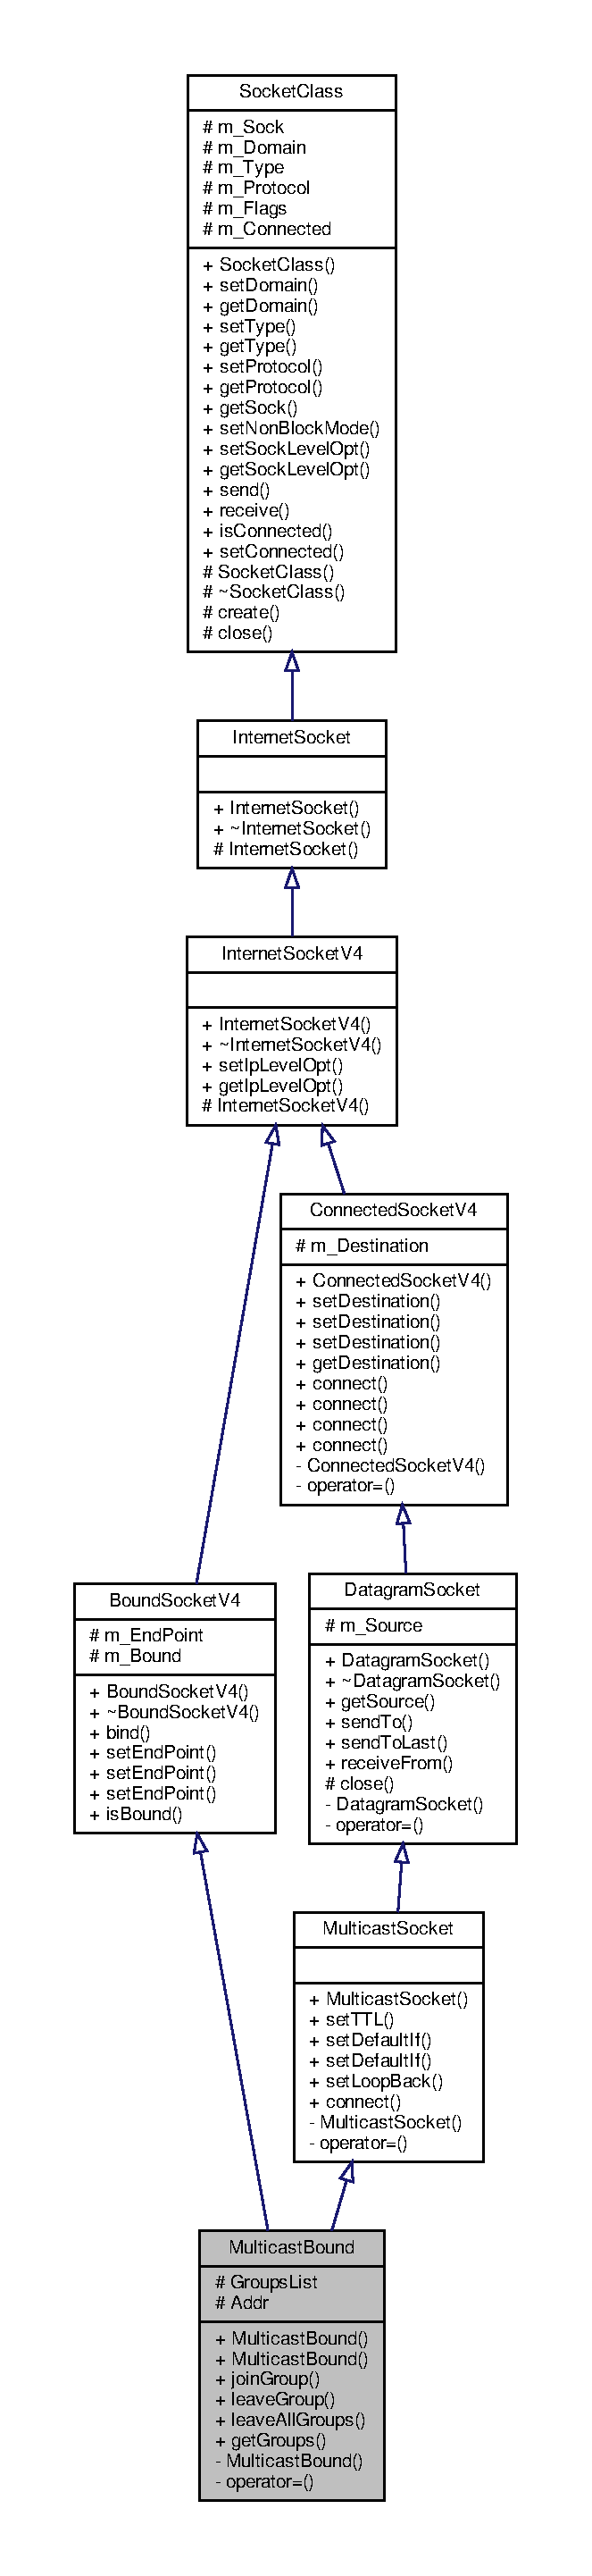
\includegraphics[height=550pt]{classMulticastBound__inherit__graph}
\end{center}
\end{figure}
\subsection*{Public Member Functions}
\begin{DoxyCompactItemize}
\item 
\hyperlink{classMulticastBound_aed105f983bf0ec03ddea66770e2622e7}{Multicast\+Bound} (short Port, in\+\_\+addr\+\_\+t Address=I\+N\+A\+D\+D\+R\+\_\+\+A\+NY)
\item 
\hyperlink{classMulticastBound_ae761776cabab795de9070aa631cbe7a7}{Multicast\+Bound} (short Port, const char $\ast$Address)
\item 
void \hyperlink{classMulticastBound_acfbbffdce81eb2930757ad6472b9b683}{join\+Group} (in\+\_\+addr\+\_\+t Group)
\item 
void \hyperlink{classMulticastBound_a85305ecf42f299160a535429563e6b94}{leave\+Group} (in\+\_\+addr\+\_\+t Group)
\item 
void \hyperlink{classMulticastBound_a3e61ea82cb090a348a1445b2c2a99dae}{leave\+All\+Groups} ()
\item 
\hyperlink{MulticastBound_8h_a9584173a620a338ea7d88264229e36dd}{Groups\+List\+Type} $\ast$ \hyperlink{classMulticastBound_a6d13e9136309c456b242cdc652e47062}{get\+Groups} ()
\end{DoxyCompactItemize}
\subsection*{Protected Attributes}
\begin{DoxyCompactItemize}
\item 
\hyperlink{MulticastBound_8h_a9584173a620a338ea7d88264229e36dd}{Groups\+List\+Type} \hyperlink{classMulticastBound_a717064ed29a84f4cc2c514eb3b1e695f}{Groups\+List}
\begin{DoxyCompactList}\small\item\em Joined multicast groups list. \end{DoxyCompactList}\item 
in\+\_\+addr\+\_\+t \hyperlink{classMulticastBound_ac7596721222c7cac2c3dcc44309aebc2}{Addr}
\begin{DoxyCompactList}\small\item\em Bound address. \end{DoxyCompactList}\end{DoxyCompactItemize}
\subsection*{Private Member Functions}
\begin{DoxyCompactItemize}
\item 
\hyperlink{classMulticastBound_ad5d067caa09a43a6eb3a6cdee5065550}{Multicast\+Bound} (\hyperlink{classMulticastBound}{Multicast\+Bound} \&s)
\item 
\hyperlink{classMulticastBound}{Multicast\+Bound} \& \hyperlink{classMulticastBound_a8b956721a93be63018cc49fe04775207}{operator=} (\hyperlink{classMulticastBound}{Multicast\+Bound} \&)
\end{DoxyCompactItemize}
\subsection*{Additional Inherited Members}


\subsection{Detailed Description}
I\+Pv4 socket capable to receive multicast datagrams. 

\subsection{Constructor \& Destructor Documentation}
\mbox{\Hypertarget{classMulticastBound_aed105f983bf0ec03ddea66770e2622e7}\label{classMulticastBound_aed105f983bf0ec03ddea66770e2622e7}} 
\index{Multicast\+Bound@{Multicast\+Bound}!Multicast\+Bound@{Multicast\+Bound}}
\index{Multicast\+Bound@{Multicast\+Bound}!Multicast\+Bound@{Multicast\+Bound}}
\subsubsection{\texorpdfstring{Multicast\+Bound()}{MulticastBound()}\hspace{0.1cm}{\footnotesize\ttfamily [1/3]}}
{\footnotesize\ttfamily Multicast\+Bound\+::\+Multicast\+Bound (\begin{DoxyParamCaption}\item[{short}]{Port,  }\item[{in\+\_\+addr\+\_\+t}]{Address = {\ttfamily INADDR\+\_\+ANY} }\end{DoxyParamCaption})}

Constructor. 
\begin{DoxyParams}{Parameters}
{\em Port} & \+: port number for bind in network byte order. \\
\hline
{\em Address} & \+: address for bind in network byte order. \\
\hline
\end{DoxyParams}

\begin{DoxyExceptions}{Exceptions}
{\em Sock\+Exception.} & \\
\hline
\end{DoxyExceptions}
\mbox{\Hypertarget{classMulticastBound_ae761776cabab795de9070aa631cbe7a7}\label{classMulticastBound_ae761776cabab795de9070aa631cbe7a7}} 
\index{Multicast\+Bound@{Multicast\+Bound}!Multicast\+Bound@{Multicast\+Bound}}
\index{Multicast\+Bound@{Multicast\+Bound}!Multicast\+Bound@{Multicast\+Bound}}
\subsubsection{\texorpdfstring{Multicast\+Bound()}{MulticastBound()}\hspace{0.1cm}{\footnotesize\ttfamily [2/3]}}
{\footnotesize\ttfamily Multicast\+Bound\+::\+Multicast\+Bound (\begin{DoxyParamCaption}\item[{short}]{Port,  }\item[{const char $\ast$}]{Address }\end{DoxyParamCaption})}

Constructor. 
\begin{DoxyParams}{Parameters}
{\em Port} & \+: port number for bind in network byte order. \\
\hline
{\em Address} & \+: address for bind in decimal dot notation. \\
\hline
\end{DoxyParams}

\begin{DoxyExceptions}{Exceptions}
{\em Sock\+Exception.} & \\
\hline
\end{DoxyExceptions}
\mbox{\Hypertarget{classMulticastBound_ad5d067caa09a43a6eb3a6cdee5065550}\label{classMulticastBound_ad5d067caa09a43a6eb3a6cdee5065550}} 
\index{Multicast\+Bound@{Multicast\+Bound}!Multicast\+Bound@{Multicast\+Bound}}
\index{Multicast\+Bound@{Multicast\+Bound}!Multicast\+Bound@{Multicast\+Bound}}
\subsubsection{\texorpdfstring{Multicast\+Bound()}{MulticastBound()}\hspace{0.1cm}{\footnotesize\ttfamily [3/3]}}
{\footnotesize\ttfamily Multicast\+Bound\+::\+Multicast\+Bound (\begin{DoxyParamCaption}\item[{\hyperlink{classMulticastBound}{Multicast\+Bound} \&}]{s }\end{DoxyParamCaption})\hspace{0.3cm}{\ttfamily [private]}}

Copy constructor. Makes the class uncopyable. 

\subsection{Member Function Documentation}
\mbox{\Hypertarget{classMulticastBound_a6d13e9136309c456b242cdc652e47062}\label{classMulticastBound_a6d13e9136309c456b242cdc652e47062}} 
\index{Multicast\+Bound@{Multicast\+Bound}!get\+Groups@{get\+Groups}}
\index{get\+Groups@{get\+Groups}!Multicast\+Bound@{Multicast\+Bound}}
\subsubsection{\texorpdfstring{get\+Groups()}{getGroups()}}
{\footnotesize\ttfamily \hyperlink{MulticastBound_8h_a9584173a620a338ea7d88264229e36dd}{Groups\+List\+Type}$\ast$ Multicast\+Bound\+::get\+Groups (\begin{DoxyParamCaption}{ }\end{DoxyParamCaption})\hspace{0.3cm}{\ttfamily [inline]}}

Get list of joined multicast groups. \begin{DoxyReturn}{Returns}
group list pointer. 
\end{DoxyReturn}
\mbox{\Hypertarget{classMulticastBound_acfbbffdce81eb2930757ad6472b9b683}\label{classMulticastBound_acfbbffdce81eb2930757ad6472b9b683}} 
\index{Multicast\+Bound@{Multicast\+Bound}!join\+Group@{join\+Group}}
\index{join\+Group@{join\+Group}!Multicast\+Bound@{Multicast\+Bound}}
\subsubsection{\texorpdfstring{join\+Group()}{joinGroup()}}
{\footnotesize\ttfamily void Multicast\+Bound\+::join\+Group (\begin{DoxyParamCaption}\item[{in\+\_\+addr\+\_\+t}]{Group }\end{DoxyParamCaption})}

Join multicast group. Param Group \+: multicast group address in network byte order. 
\begin{DoxyExceptions}{Exceptions}
{\em Sock\+Exception.} & \\
\hline
\end{DoxyExceptions}
\mbox{\Hypertarget{classMulticastBound_a3e61ea82cb090a348a1445b2c2a99dae}\label{classMulticastBound_a3e61ea82cb090a348a1445b2c2a99dae}} 
\index{Multicast\+Bound@{Multicast\+Bound}!leave\+All\+Groups@{leave\+All\+Groups}}
\index{leave\+All\+Groups@{leave\+All\+Groups}!Multicast\+Bound@{Multicast\+Bound}}
\subsubsection{\texorpdfstring{leave\+All\+Groups()}{leaveAllGroups()}}
{\footnotesize\ttfamily void Multicast\+Bound\+::leave\+All\+Groups (\begin{DoxyParamCaption}{ }\end{DoxyParamCaption})}

Leave all multicast groups previously joined. 
\begin{DoxyExceptions}{Exceptions}
{\em Sock\+Exception.} & \\
\hline
\end{DoxyExceptions}
\mbox{\Hypertarget{classMulticastBound_a85305ecf42f299160a535429563e6b94}\label{classMulticastBound_a85305ecf42f299160a535429563e6b94}} 
\index{Multicast\+Bound@{Multicast\+Bound}!leave\+Group@{leave\+Group}}
\index{leave\+Group@{leave\+Group}!Multicast\+Bound@{Multicast\+Bound}}
\subsubsection{\texorpdfstring{leave\+Group()}{leaveGroup()}}
{\footnotesize\ttfamily void Multicast\+Bound\+::leave\+Group (\begin{DoxyParamCaption}\item[{in\+\_\+addr\+\_\+t}]{Group }\end{DoxyParamCaption})}

Leave multicast group. Param Group \+: multicast group address in network byte order. 
\begin{DoxyExceptions}{Exceptions}
{\em Sock\+Exception.} & \\
\hline
\end{DoxyExceptions}
\mbox{\Hypertarget{classMulticastBound_a8b956721a93be63018cc49fe04775207}\label{classMulticastBound_a8b956721a93be63018cc49fe04775207}} 
\index{Multicast\+Bound@{Multicast\+Bound}!operator=@{operator=}}
\index{operator=@{operator=}!Multicast\+Bound@{Multicast\+Bound}}
\subsubsection{\texorpdfstring{operator=()}{operator=()}}
{\footnotesize\ttfamily \hyperlink{classMulticastBound}{Multicast\+Bound}\& Multicast\+Bound\+::operator= (\begin{DoxyParamCaption}\item[{\hyperlink{classMulticastBound}{Multicast\+Bound} \&}]{ }\end{DoxyParamCaption})\hspace{0.3cm}{\ttfamily [private]}}

Operator assign. Makes the class uncopyable. 

\subsection{Member Data Documentation}
\mbox{\Hypertarget{classMulticastBound_ac7596721222c7cac2c3dcc44309aebc2}\label{classMulticastBound_ac7596721222c7cac2c3dcc44309aebc2}} 
\index{Multicast\+Bound@{Multicast\+Bound}!Addr@{Addr}}
\index{Addr@{Addr}!Multicast\+Bound@{Multicast\+Bound}}
\subsubsection{\texorpdfstring{Addr}{Addr}}
{\footnotesize\ttfamily in\+\_\+addr\+\_\+t Multicast\+Bound\+::\+Addr\hspace{0.3cm}{\ttfamily [protected]}}



Bound address. 

\mbox{\Hypertarget{classMulticastBound_a717064ed29a84f4cc2c514eb3b1e695f}\label{classMulticastBound_a717064ed29a84f4cc2c514eb3b1e695f}} 
\index{Multicast\+Bound@{Multicast\+Bound}!Groups\+List@{Groups\+List}}
\index{Groups\+List@{Groups\+List}!Multicast\+Bound@{Multicast\+Bound}}
\subsubsection{\texorpdfstring{Groups\+List}{GroupsList}}
{\footnotesize\ttfamily \hyperlink{MulticastBound_8h_a9584173a620a338ea7d88264229e36dd}{Groups\+List\+Type} Multicast\+Bound\+::\+Groups\+List\hspace{0.3cm}{\ttfamily [protected]}}



Joined multicast groups list. 



The documentation for this class was generated from the following files\+:\begin{DoxyCompactItemize}
\item 
\hyperlink{MulticastBound_8h}{Multicast\+Bound.\+h}\item 
\hyperlink{MulticastBound_8cpp}{Multicast\+Bound.\+cpp}\end{DoxyCompactItemize}

\hypertarget{classMulticastBoundV6}{}\section{Multicast\+Bound\+V6 Class Reference}
\label{classMulticastBoundV6}\index{Multicast\+Bound\+V6@{Multicast\+Bound\+V6}}


I\+Pv4 socket capable to receive multicast datagrams.  




{\ttfamily \#include $<$Multicast\+Bound\+V6.\+h$>$}



Inheritance diagram for Multicast\+Bound\+V6\+:\nopagebreak
\begin{figure}[H]
\begin{center}
\leavevmode
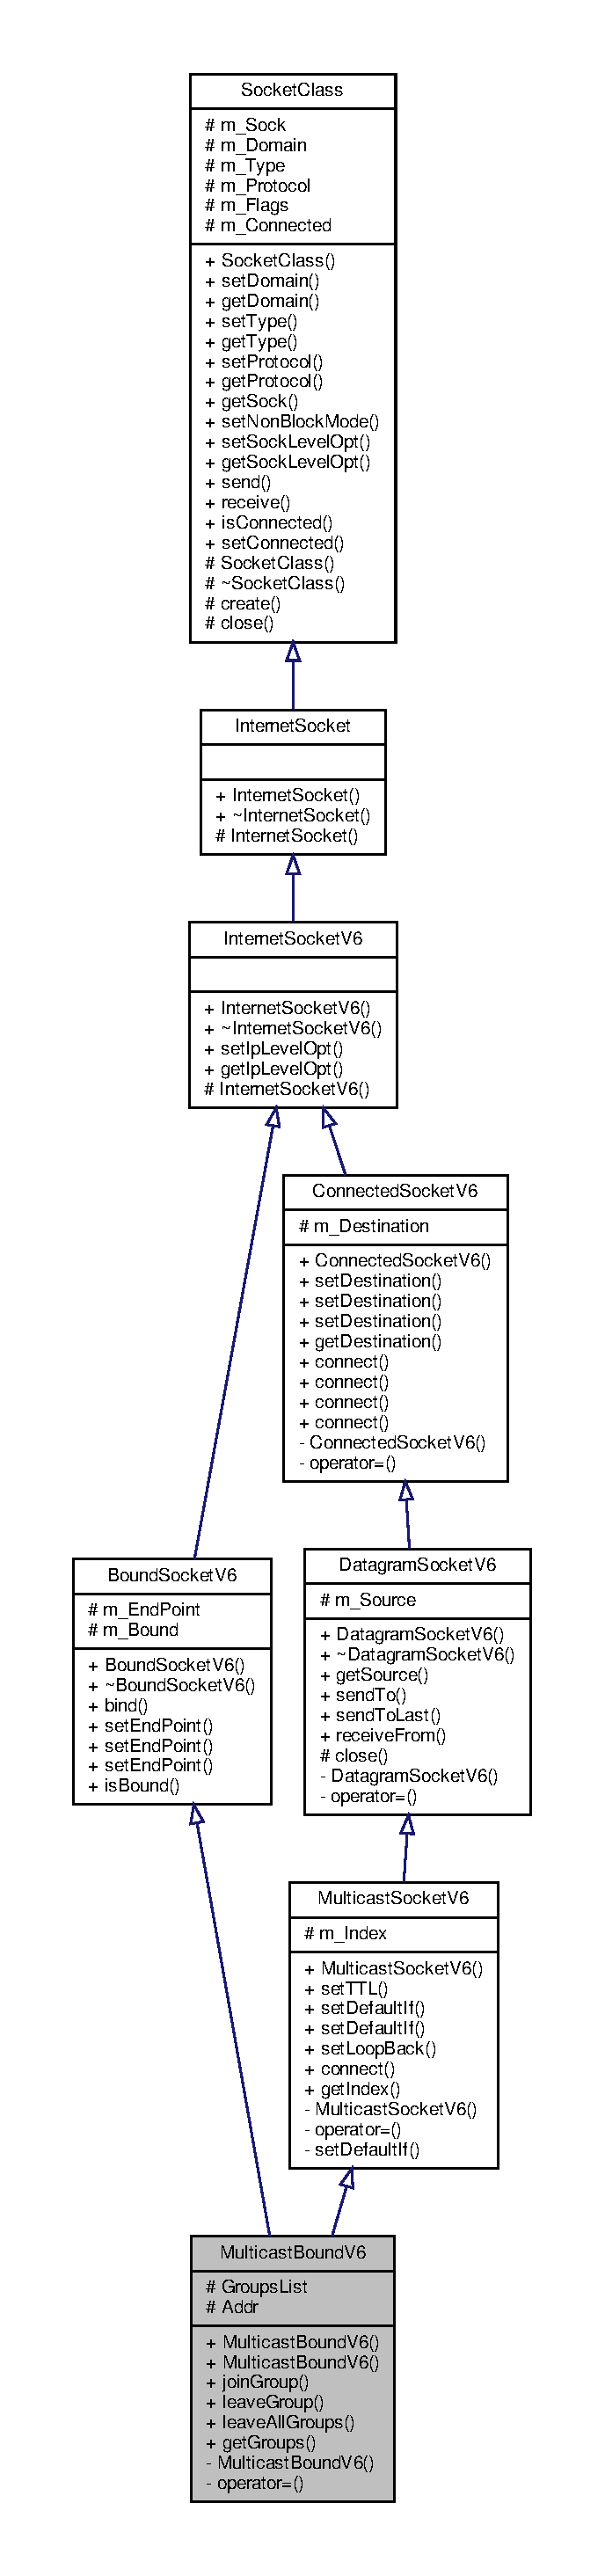
\includegraphics[height=550pt]{classMulticastBoundV6__inherit__graph}
\end{center}
\end{figure}
\subsection*{Public Member Functions}
\begin{DoxyCompactItemize}
\item 
\hyperlink{classMulticastBoundV6_aeff8613d8b6c8c7e5ecbdbbc2b73bf8a}{Multicast\+Bound\+V6} (short Port, in6\+\_\+addr Address=in6addr\+\_\+any)
\item 
\hyperlink{classMulticastBoundV6_a90c23a309b94b8e997dff8177a478ab2}{Multicast\+Bound\+V6} (short Port, const char $\ast$Address)
\item 
void \hyperlink{classMulticastBoundV6_a8ad4a26d4469cc1ffd3f451d4ce8ebd9}{join\+Group} (in6\+\_\+addr Group)
\item 
void \hyperlink{classMulticastBoundV6_a7264da712de9e131b3a3ab1e8a86942a}{leave\+Group} (in6\+\_\+addr Group)
\item 
void \hyperlink{classMulticastBoundV6_a94ea6a1c81af951376b82d23d58a7acd}{leave\+All\+Groups} ()
\item 
\hyperlink{MulticastBound_8h_a9584173a620a338ea7d88264229e36dd}{Groups\+List\+Type} $\ast$ \hyperlink{classMulticastBoundV6_afcb2560007274a519ed11101bc95fbee}{get\+Groups} ()
\end{DoxyCompactItemize}
\subsection*{Protected Attributes}
\begin{DoxyCompactItemize}
\item 
\hyperlink{MulticastBound_8h_a9584173a620a338ea7d88264229e36dd}{Groups\+List\+Type} \hyperlink{classMulticastBoundV6_a6ccdbb56f54017f5a4372eb816b5b077}{Groups\+List}
\begin{DoxyCompactList}\small\item\em Joined multicast groups list. \end{DoxyCompactList}\item 
in6\+\_\+addr \hyperlink{classMulticastBoundV6_a792a38740cf29b50fb74785b12358988}{Addr}
\begin{DoxyCompactList}\small\item\em Bound address. \end{DoxyCompactList}\end{DoxyCompactItemize}
\subsection*{Private Member Functions}
\begin{DoxyCompactItemize}
\item 
\hyperlink{classMulticastBoundV6_a207359a0e4b496dfe9a00ceb33be4c18}{Multicast\+Bound\+V6} (\hyperlink{classMulticastBoundV6}{Multicast\+Bound\+V6} \&s)
\item 
\hyperlink{classMulticastBoundV6}{Multicast\+Bound\+V6} \& \hyperlink{classMulticastBoundV6_a5bcf54776fe97dd2ffd26a36de092284}{operator=} (\hyperlink{classMulticastBoundV6}{Multicast\+Bound\+V6} \&)
\end{DoxyCompactItemize}
\subsection*{Additional Inherited Members}


\subsection{Detailed Description}
I\+Pv4 socket capable to receive multicast datagrams. 

\subsection{Constructor \& Destructor Documentation}
\mbox{\Hypertarget{classMulticastBoundV6_aeff8613d8b6c8c7e5ecbdbbc2b73bf8a}\label{classMulticastBoundV6_aeff8613d8b6c8c7e5ecbdbbc2b73bf8a}} 
\index{Multicast\+Bound\+V6@{Multicast\+Bound\+V6}!Multicast\+Bound\+V6@{Multicast\+Bound\+V6}}
\index{Multicast\+Bound\+V6@{Multicast\+Bound\+V6}!Multicast\+Bound\+V6@{Multicast\+Bound\+V6}}
\subsubsection{\texorpdfstring{Multicast\+Bound\+V6()}{MulticastBoundV6()}\hspace{0.1cm}{\footnotesize\ttfamily [1/3]}}
{\footnotesize\ttfamily Multicast\+Bound\+V6\+::\+Multicast\+Bound\+V6 (\begin{DoxyParamCaption}\item[{short}]{Port,  }\item[{in6\+\_\+addr}]{Address = {\ttfamily in6addr\+\_\+any} }\end{DoxyParamCaption})}

Constructor. 
\begin{DoxyParams}{Parameters}
{\em Port} & \+: port number for bind in network byte order. \\
\hline
{\em Address} & \+: address for bind in network byte order. \\
\hline
\end{DoxyParams}

\begin{DoxyExceptions}{Exceptions}
{\em Sock\+Exception.} & \\
\hline
\end{DoxyExceptions}
\mbox{\Hypertarget{classMulticastBoundV6_a90c23a309b94b8e997dff8177a478ab2}\label{classMulticastBoundV6_a90c23a309b94b8e997dff8177a478ab2}} 
\index{Multicast\+Bound\+V6@{Multicast\+Bound\+V6}!Multicast\+Bound\+V6@{Multicast\+Bound\+V6}}
\index{Multicast\+Bound\+V6@{Multicast\+Bound\+V6}!Multicast\+Bound\+V6@{Multicast\+Bound\+V6}}
\subsubsection{\texorpdfstring{Multicast\+Bound\+V6()}{MulticastBoundV6()}\hspace{0.1cm}{\footnotesize\ttfamily [2/3]}}
{\footnotesize\ttfamily Multicast\+Bound\+V6\+::\+Multicast\+Bound\+V6 (\begin{DoxyParamCaption}\item[{short}]{Port,  }\item[{const char $\ast$}]{Address }\end{DoxyParamCaption})}

Constructor. 
\begin{DoxyParams}{Parameters}
{\em Port} & \+: port number for bind in network byte order. \\
\hline
{\em Address} & \+: address for bind in textual notation. \\
\hline
\end{DoxyParams}

\begin{DoxyExceptions}{Exceptions}
{\em Sock\+Exception.} & \\
\hline
\end{DoxyExceptions}
\mbox{\Hypertarget{classMulticastBoundV6_a207359a0e4b496dfe9a00ceb33be4c18}\label{classMulticastBoundV6_a207359a0e4b496dfe9a00ceb33be4c18}} 
\index{Multicast\+Bound\+V6@{Multicast\+Bound\+V6}!Multicast\+Bound\+V6@{Multicast\+Bound\+V6}}
\index{Multicast\+Bound\+V6@{Multicast\+Bound\+V6}!Multicast\+Bound\+V6@{Multicast\+Bound\+V6}}
\subsubsection{\texorpdfstring{Multicast\+Bound\+V6()}{MulticastBoundV6()}\hspace{0.1cm}{\footnotesize\ttfamily [3/3]}}
{\footnotesize\ttfamily Multicast\+Bound\+V6\+::\+Multicast\+Bound\+V6 (\begin{DoxyParamCaption}\item[{\hyperlink{classMulticastBoundV6}{Multicast\+Bound\+V6} \&}]{s }\end{DoxyParamCaption})\hspace{0.3cm}{\ttfamily [private]}}

Copy constructor. Makes the class uncopyable. 

\subsection{Member Function Documentation}
\mbox{\Hypertarget{classMulticastBoundV6_afcb2560007274a519ed11101bc95fbee}\label{classMulticastBoundV6_afcb2560007274a519ed11101bc95fbee}} 
\index{Multicast\+Bound\+V6@{Multicast\+Bound\+V6}!get\+Groups@{get\+Groups}}
\index{get\+Groups@{get\+Groups}!Multicast\+Bound\+V6@{Multicast\+Bound\+V6}}
\subsubsection{\texorpdfstring{get\+Groups()}{getGroups()}}
{\footnotesize\ttfamily \hyperlink{MulticastBound_8h_a9584173a620a338ea7d88264229e36dd}{Groups\+List\+Type}$\ast$ Multicast\+Bound\+V6\+::get\+Groups (\begin{DoxyParamCaption}{ }\end{DoxyParamCaption})\hspace{0.3cm}{\ttfamily [inline]}}

Get list of joined multicast groups. \begin{DoxyReturn}{Returns}
group list pointer. 
\end{DoxyReturn}
\mbox{\Hypertarget{classMulticastBoundV6_a8ad4a26d4469cc1ffd3f451d4ce8ebd9}\label{classMulticastBoundV6_a8ad4a26d4469cc1ffd3f451d4ce8ebd9}} 
\index{Multicast\+Bound\+V6@{Multicast\+Bound\+V6}!join\+Group@{join\+Group}}
\index{join\+Group@{join\+Group}!Multicast\+Bound\+V6@{Multicast\+Bound\+V6}}
\subsubsection{\texorpdfstring{join\+Group()}{joinGroup()}}
{\footnotesize\ttfamily void Multicast\+Bound\+V6\+::join\+Group (\begin{DoxyParamCaption}\item[{in6\+\_\+addr}]{Group }\end{DoxyParamCaption})}

Join multicast group. Param Group \+: multicast group address in network byte order. 
\begin{DoxyExceptions}{Exceptions}
{\em Sock\+Exception.} & \\
\hline
\end{DoxyExceptions}
\mbox{\Hypertarget{classMulticastBoundV6_a94ea6a1c81af951376b82d23d58a7acd}\label{classMulticastBoundV6_a94ea6a1c81af951376b82d23d58a7acd}} 
\index{Multicast\+Bound\+V6@{Multicast\+Bound\+V6}!leave\+All\+Groups@{leave\+All\+Groups}}
\index{leave\+All\+Groups@{leave\+All\+Groups}!Multicast\+Bound\+V6@{Multicast\+Bound\+V6}}
\subsubsection{\texorpdfstring{leave\+All\+Groups()}{leaveAllGroups()}}
{\footnotesize\ttfamily void Multicast\+Bound\+V6\+::leave\+All\+Groups (\begin{DoxyParamCaption}{ }\end{DoxyParamCaption})}

Leave all multicast groups previously joined. 
\begin{DoxyExceptions}{Exceptions}
{\em Sock\+Exception.} & \\
\hline
\end{DoxyExceptions}
\mbox{\Hypertarget{classMulticastBoundV6_a7264da712de9e131b3a3ab1e8a86942a}\label{classMulticastBoundV6_a7264da712de9e131b3a3ab1e8a86942a}} 
\index{Multicast\+Bound\+V6@{Multicast\+Bound\+V6}!leave\+Group@{leave\+Group}}
\index{leave\+Group@{leave\+Group}!Multicast\+Bound\+V6@{Multicast\+Bound\+V6}}
\subsubsection{\texorpdfstring{leave\+Group()}{leaveGroup()}}
{\footnotesize\ttfamily void Multicast\+Bound\+V6\+::leave\+Group (\begin{DoxyParamCaption}\item[{in6\+\_\+addr}]{Group }\end{DoxyParamCaption})}

Leave multicast group. Param Group \+: multicast group address in network byte order. 
\begin{DoxyExceptions}{Exceptions}
{\em Sock\+Exception.} & \\
\hline
\end{DoxyExceptions}
\mbox{\Hypertarget{classMulticastBoundV6_a5bcf54776fe97dd2ffd26a36de092284}\label{classMulticastBoundV6_a5bcf54776fe97dd2ffd26a36de092284}} 
\index{Multicast\+Bound\+V6@{Multicast\+Bound\+V6}!operator=@{operator=}}
\index{operator=@{operator=}!Multicast\+Bound\+V6@{Multicast\+Bound\+V6}}
\subsubsection{\texorpdfstring{operator=()}{operator=()}}
{\footnotesize\ttfamily \hyperlink{classMulticastBoundV6}{Multicast\+Bound\+V6}\& Multicast\+Bound\+V6\+::operator= (\begin{DoxyParamCaption}\item[{\hyperlink{classMulticastBoundV6}{Multicast\+Bound\+V6} \&}]{ }\end{DoxyParamCaption})\hspace{0.3cm}{\ttfamily [private]}}

Operator assign. Makes the class uncopyable. 

\subsection{Member Data Documentation}
\mbox{\Hypertarget{classMulticastBoundV6_a792a38740cf29b50fb74785b12358988}\label{classMulticastBoundV6_a792a38740cf29b50fb74785b12358988}} 
\index{Multicast\+Bound\+V6@{Multicast\+Bound\+V6}!Addr@{Addr}}
\index{Addr@{Addr}!Multicast\+Bound\+V6@{Multicast\+Bound\+V6}}
\subsubsection{\texorpdfstring{Addr}{Addr}}
{\footnotesize\ttfamily in6\+\_\+addr Multicast\+Bound\+V6\+::\+Addr\hspace{0.3cm}{\ttfamily [protected]}}



Bound address. 

\mbox{\Hypertarget{classMulticastBoundV6_a6ccdbb56f54017f5a4372eb816b5b077}\label{classMulticastBoundV6_a6ccdbb56f54017f5a4372eb816b5b077}} 
\index{Multicast\+Bound\+V6@{Multicast\+Bound\+V6}!Groups\+List@{Groups\+List}}
\index{Groups\+List@{Groups\+List}!Multicast\+Bound\+V6@{Multicast\+Bound\+V6}}
\subsubsection{\texorpdfstring{Groups\+List}{GroupsList}}
{\footnotesize\ttfamily \hyperlink{MulticastBound_8h_a9584173a620a338ea7d88264229e36dd}{Groups\+List\+Type} Multicast\+Bound\+V6\+::\+Groups\+List\hspace{0.3cm}{\ttfamily [protected]}}



Joined multicast groups list. 



The documentation for this class was generated from the following files\+:\begin{DoxyCompactItemize}
\item 
\hyperlink{MulticastBoundV6_8h}{Multicast\+Bound\+V6.\+h}\item 
\hyperlink{MulticastBoundV6_8cpp}{Multicast\+Bound\+V6.\+cpp}\end{DoxyCompactItemize}

\hypertarget{classMulticastSocket}{}\section{Multicast\+Socket Class Reference}
\label{classMulticastSocket}\index{Multicast\+Socket@{Multicast\+Socket}}


I\+Pv4 datagram socket capable to send multicast datagrams.  




{\ttfamily \#include $<$Multicast\+Socket.\+h$>$}



Inheritance diagram for Multicast\+Socket\+:\nopagebreak
\begin{figure}[H]
\begin{center}
\leavevmode
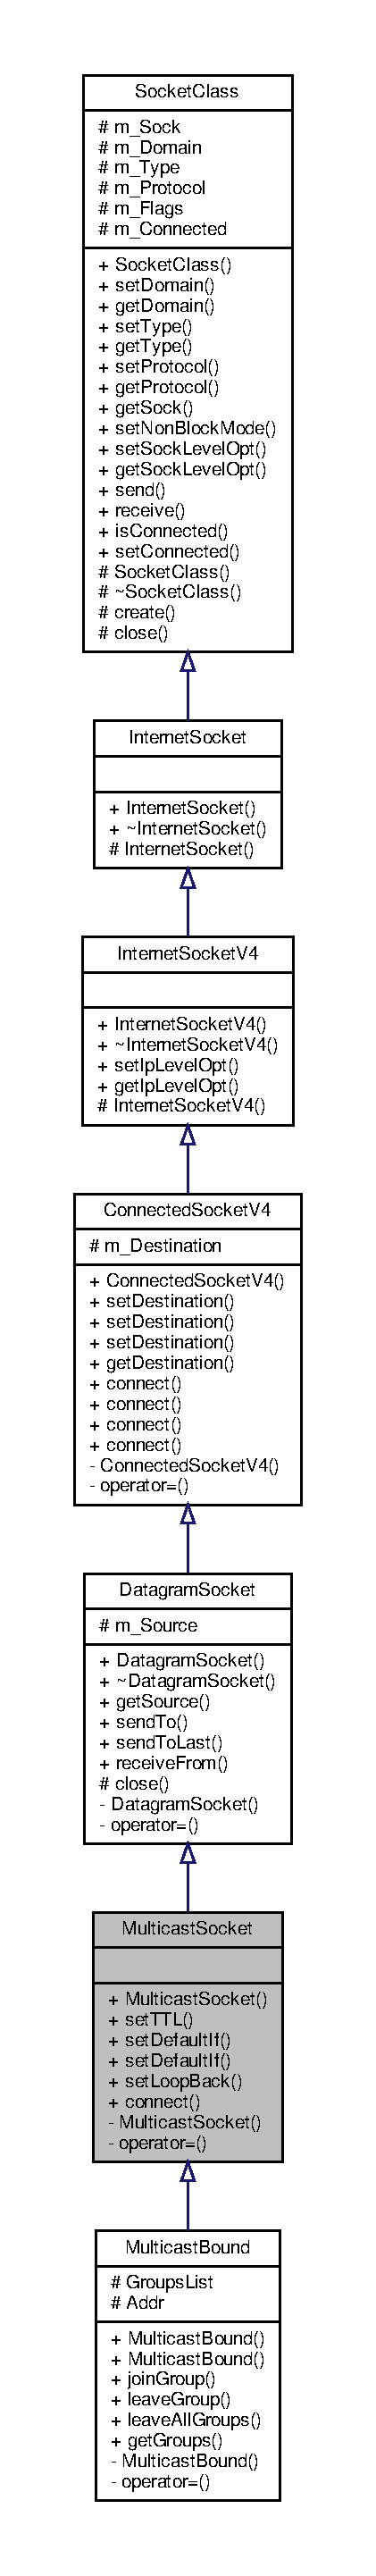
\includegraphics[height=550pt]{classMulticastSocket__inherit__graph}
\end{center}
\end{figure}
\subsection*{Public Member Functions}
\begin{DoxyCompactItemize}
\item 
\hyperlink{classMulticastSocket_a757cf27883d58403d8c407ac6e1b9abb}{Multicast\+Socket} ()
\item 
void \hyperlink{classMulticastSocket_abf3fae43ee2575adfc7c90ee31b1fc0a}{set\+T\+TL} (unsigned char ttl)
\item 
void \hyperlink{classMulticastSocket_a64399ca9f96c7f8fcf453c6233d17165}{set\+Default\+If} (in\+\_\+addr\+\_\+t Address)
\item 
void \hyperlink{classMulticastSocket_abd769428b74a9dc88fca8c27bb53da1a}{set\+Default\+If} (const char $\ast$Address)
\item 
void \hyperlink{classMulticastSocket_a3f30553f778aa0bf541fc8d1c772e2e2}{set\+Loop\+Back} (bool On=true)
\item 
virtual void \hyperlink{classMulticastSocket_a30ffd3d7fe782c2d74d69d994e465a4d}{connect} ()
\end{DoxyCompactItemize}
\subsection*{Private Member Functions}
\begin{DoxyCompactItemize}
\item 
\hyperlink{classMulticastSocket_a85ca1e8e1c4c726d906393eec29adf00}{Multicast\+Socket} (\hyperlink{classMulticastSocket}{Multicast\+Socket} \&s)
\item 
\hyperlink{classMulticastSocket}{Multicast\+Socket} \& \hyperlink{classMulticastSocket_a644a16ae716496f9d92389f7a9e80b3e}{operator=} (\hyperlink{classMulticastSocket}{Multicast\+Socket} \&)
\end{DoxyCompactItemize}
\subsection*{Additional Inherited Members}


\subsection{Detailed Description}
I\+Pv4 datagram socket capable to send multicast datagrams. 

\subsection{Constructor \& Destructor Documentation}
\mbox{\Hypertarget{classMulticastSocket_a757cf27883d58403d8c407ac6e1b9abb}\label{classMulticastSocket_a757cf27883d58403d8c407ac6e1b9abb}} 
\index{Multicast\+Socket@{Multicast\+Socket}!Multicast\+Socket@{Multicast\+Socket}}
\index{Multicast\+Socket@{Multicast\+Socket}!Multicast\+Socket@{Multicast\+Socket}}
\subsubsection{\texorpdfstring{Multicast\+Socket()}{MulticastSocket()}\hspace{0.1cm}{\footnotesize\ttfamily [1/2]}}
{\footnotesize\ttfamily Multicast\+Socket\+::\+Multicast\+Socket (\begin{DoxyParamCaption}{ }\end{DoxyParamCaption})\hspace{0.3cm}{\ttfamily [inline]}}

Constructor. 
\begin{DoxyExceptions}{Exceptions}
{\em Sock\+Exception.} & \\
\hline
\end{DoxyExceptions}
\mbox{\Hypertarget{classMulticastSocket_a85ca1e8e1c4c726d906393eec29adf00}\label{classMulticastSocket_a85ca1e8e1c4c726d906393eec29adf00}} 
\index{Multicast\+Socket@{Multicast\+Socket}!Multicast\+Socket@{Multicast\+Socket}}
\index{Multicast\+Socket@{Multicast\+Socket}!Multicast\+Socket@{Multicast\+Socket}}
\subsubsection{\texorpdfstring{Multicast\+Socket()}{MulticastSocket()}\hspace{0.1cm}{\footnotesize\ttfamily [2/2]}}
{\footnotesize\ttfamily Multicast\+Socket\+::\+Multicast\+Socket (\begin{DoxyParamCaption}\item[{\hyperlink{classMulticastSocket}{Multicast\+Socket} \&}]{s }\end{DoxyParamCaption})\hspace{0.3cm}{\ttfamily [private]}}

Copy constructor. Makes the class uncopyable. 

\subsection{Member Function Documentation}
\mbox{\Hypertarget{classMulticastSocket_a30ffd3d7fe782c2d74d69d994e465a4d}\label{classMulticastSocket_a30ffd3d7fe782c2d74d69d994e465a4d}} 
\index{Multicast\+Socket@{Multicast\+Socket}!connect@{connect}}
\index{connect@{connect}!Multicast\+Socket@{Multicast\+Socket}}
\subsubsection{\texorpdfstring{connect()}{connect()}}
{\footnotesize\ttfamily virtual void Multicast\+Socket\+::connect (\begin{DoxyParamCaption}{ }\end{DoxyParamCaption})\hspace{0.3cm}{\ttfamily [inline]}, {\ttfamily [virtual]}}

Connect the socket. Implements pure virtual function of base class. Has no meaning for this particular class. 
\begin{DoxyExceptions}{Exceptions}
{\em Sock\+Exception.} & \\
\hline
\end{DoxyExceptions}


Reimplemented from \hyperlink{classConnectedSocketV4_a034d0c949fa1a0f14c136f839915d1a4}{Connected\+Socket\+V4}.

\mbox{\Hypertarget{classMulticastSocket_a644a16ae716496f9d92389f7a9e80b3e}\label{classMulticastSocket_a644a16ae716496f9d92389f7a9e80b3e}} 
\index{Multicast\+Socket@{Multicast\+Socket}!operator=@{operator=}}
\index{operator=@{operator=}!Multicast\+Socket@{Multicast\+Socket}}
\subsubsection{\texorpdfstring{operator=()}{operator=()}}
{\footnotesize\ttfamily \hyperlink{classMulticastSocket}{Multicast\+Socket}\& Multicast\+Socket\+::operator= (\begin{DoxyParamCaption}\item[{\hyperlink{classMulticastSocket}{Multicast\+Socket} \&}]{ }\end{DoxyParamCaption})\hspace{0.3cm}{\ttfamily [private]}}

Operator assign. Makes the class uncopyable. \mbox{\Hypertarget{classMulticastSocket_a64399ca9f96c7f8fcf453c6233d17165}\label{classMulticastSocket_a64399ca9f96c7f8fcf453c6233d17165}} 
\index{Multicast\+Socket@{Multicast\+Socket}!set\+Default\+If@{set\+Default\+If}}
\index{set\+Default\+If@{set\+Default\+If}!Multicast\+Socket@{Multicast\+Socket}}
\subsubsection{\texorpdfstring{set\+Default\+If()}{setDefaultIf()}\hspace{0.1cm}{\footnotesize\ttfamily [1/2]}}
{\footnotesize\ttfamily void Multicast\+Socket\+::set\+Default\+If (\begin{DoxyParamCaption}\item[{in\+\_\+addr\+\_\+t}]{Address }\end{DoxyParamCaption})}

Set default network interface. 
\begin{DoxyParams}{Parameters}
{\em Address} & \+: address of default network interface in network byte order. \\
\hline
\end{DoxyParams}

\begin{DoxyExceptions}{Exceptions}
{\em Sock\+Exception.} & \\
\hline
\end{DoxyExceptions}
\mbox{\Hypertarget{classMulticastSocket_abd769428b74a9dc88fca8c27bb53da1a}\label{classMulticastSocket_abd769428b74a9dc88fca8c27bb53da1a}} 
\index{Multicast\+Socket@{Multicast\+Socket}!set\+Default\+If@{set\+Default\+If}}
\index{set\+Default\+If@{set\+Default\+If}!Multicast\+Socket@{Multicast\+Socket}}
\subsubsection{\texorpdfstring{set\+Default\+If()}{setDefaultIf()}\hspace{0.1cm}{\footnotesize\ttfamily [2/2]}}
{\footnotesize\ttfamily void Multicast\+Socket\+::set\+Default\+If (\begin{DoxyParamCaption}\item[{const char $\ast$}]{Address }\end{DoxyParamCaption})}

Set default network interface. 
\begin{DoxyParams}{Parameters}
{\em Address} & \+: address of default network interface in decilmal dot notation. \\
\hline
\end{DoxyParams}

\begin{DoxyExceptions}{Exceptions}
{\em Sock\+Exception.} & \\
\hline
\end{DoxyExceptions}
\mbox{\Hypertarget{classMulticastSocket_a3f30553f778aa0bf541fc8d1c772e2e2}\label{classMulticastSocket_a3f30553f778aa0bf541fc8d1c772e2e2}} 
\index{Multicast\+Socket@{Multicast\+Socket}!set\+Loop\+Back@{set\+Loop\+Back}}
\index{set\+Loop\+Back@{set\+Loop\+Back}!Multicast\+Socket@{Multicast\+Socket}}
\subsubsection{\texorpdfstring{set\+Loop\+Back()}{setLoopBack()}}
{\footnotesize\ttfamily void Multicast\+Socket\+::set\+Loop\+Back (\begin{DoxyParamCaption}\item[{bool}]{On = {\ttfamily true} }\end{DoxyParamCaption})}

Switch on or off loppback for sent multicasts. 
\begin{DoxyParams}{Parameters}
{\em On} & \+: lopback on/off. \\
\hline
\end{DoxyParams}

\begin{DoxyExceptions}{Exceptions}
{\em Sock\+Exception.} & \\
\hline
\end{DoxyExceptions}
\mbox{\Hypertarget{classMulticastSocket_abf3fae43ee2575adfc7c90ee31b1fc0a}\label{classMulticastSocket_abf3fae43ee2575adfc7c90ee31b1fc0a}} 
\index{Multicast\+Socket@{Multicast\+Socket}!set\+T\+TL@{set\+T\+TL}}
\index{set\+T\+TL@{set\+T\+TL}!Multicast\+Socket@{Multicast\+Socket}}
\subsubsection{\texorpdfstring{set\+T\+T\+L()}{setTTL()}}
{\footnotesize\ttfamily void Multicast\+Socket\+::set\+T\+TL (\begin{DoxyParamCaption}\item[{unsigned char}]{ttl }\end{DoxyParamCaption})}

Set Time-\/\+To-\/\+Live for sent multicasts. 
\begin{DoxyParams}{Parameters}
{\em ttl} & \+: T\+TL number. \\
\hline
\end{DoxyParams}

\begin{DoxyExceptions}{Exceptions}
{\em Sock\+Exception.} & \\
\hline
\end{DoxyExceptions}


The documentation for this class was generated from the following files\+:\begin{DoxyCompactItemize}
\item 
\hyperlink{MulticastSocket_8h}{Multicast\+Socket.\+h}\item 
\hyperlink{MulticastSocket_8cpp}{Multicast\+Socket.\+cpp}\end{DoxyCompactItemize}

\hypertarget{classMulticastSocketV6}{}\section{Multicast\+Socket\+V6 Class Reference}
\label{classMulticastSocketV6}\index{Multicast\+Socket\+V6@{Multicast\+Socket\+V6}}


I\+Pv6 datagram socket capable to send multicast datagrams.  




{\ttfamily \#include $<$Multicast\+Socket\+V6.\+h$>$}



Inheritance diagram for Multicast\+Socket\+V6\+:\nopagebreak
\begin{figure}[H]
\begin{center}
\leavevmode
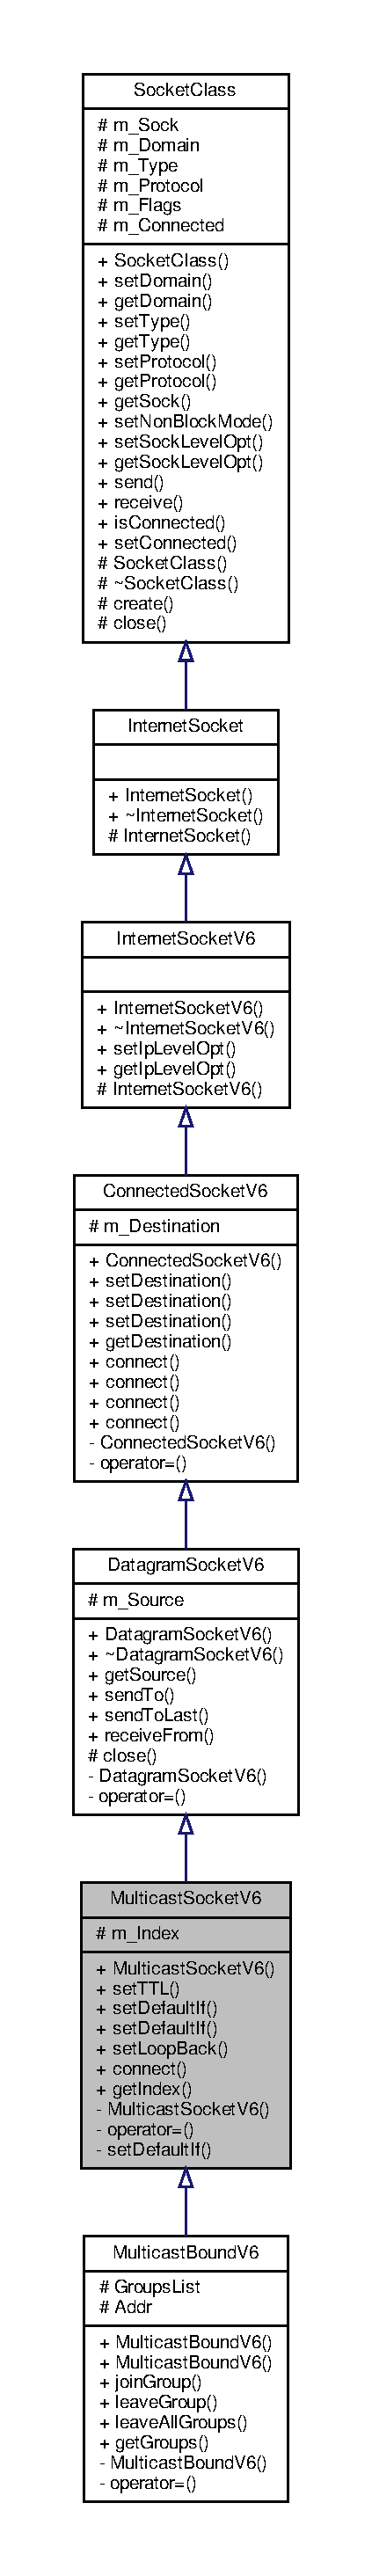
\includegraphics[height=550pt]{classMulticastSocketV6__inherit__graph}
\end{center}
\end{figure}
\subsection*{Public Member Functions}
\begin{DoxyCompactItemize}
\item 
\hyperlink{classMulticastSocketV6_ad99bb6fa0274bc92f4a342c004b395a2}{Multicast\+Socket\+V6} ()
\item 
void \hyperlink{classMulticastSocketV6_af33892d079526e17dfe7cac4128bc0d1}{set\+T\+TL} (unsigned char ttl)
\item 
void \hyperlink{classMulticastSocketV6_a79e2bd2544a73c01cc7e8c8b998da4e1}{set\+Default\+If} (in6\+\_\+addr Address)
\item 
void \hyperlink{classMulticastSocketV6_ad7534d71b628f9be4af98161cd35bdf9}{set\+Default\+If} (const char $\ast$Address)
\item 
void \hyperlink{classMulticastSocketV6_a04dea92292a94e6f395de06edf063711}{set\+Loop\+Back} (bool On=true)
\item 
virtual void \hyperlink{classMulticastSocketV6_a81b62a13aff687c5b94b8f8a946c58ed}{connect} ()
\item 
unsigned int \hyperlink{classMulticastSocketV6_a6f8366a51c3bb4c9403ec29f84432db0}{get\+Index} ()
\end{DoxyCompactItemize}
\subsection*{Protected Attributes}
\begin{DoxyCompactItemize}
\item 
unsigned int \hyperlink{classMulticastSocketV6_a97955011956119b7e551c3070f521f93}{m\+\_\+\+Index}
\begin{DoxyCompactList}\small\item\em I\+Pv6 interface index. \end{DoxyCompactList}\end{DoxyCompactItemize}
\subsection*{Private Member Functions}
\begin{DoxyCompactItemize}
\item 
\hyperlink{classMulticastSocketV6_a2a28ad5ec5326ce88700f6518eba6699}{Multicast\+Socket\+V6} (\hyperlink{classMulticastSocketV6}{Multicast\+Socket\+V6} \&s)
\item 
\hyperlink{classMulticastSocketV6}{Multicast\+Socket\+V6} \& \hyperlink{classMulticastSocketV6_a12383da396c4492f43fc9c0dfeb511b6}{operator=} (\hyperlink{classMulticastSocketV6}{Multicast\+Socket\+V6} \&)
\item 
void \hyperlink{classMulticastSocketV6_a4e211b18653d1a8ce29651068293960b}{set\+Default\+If} (unsigned int Index)
\end{DoxyCompactItemize}
\subsection*{Additional Inherited Members}


\subsection{Detailed Description}
I\+Pv6 datagram socket capable to send multicast datagrams. 

\subsection{Constructor \& Destructor Documentation}
\mbox{\Hypertarget{classMulticastSocketV6_ad99bb6fa0274bc92f4a342c004b395a2}\label{classMulticastSocketV6_ad99bb6fa0274bc92f4a342c004b395a2}} 
\index{Multicast\+Socket\+V6@{Multicast\+Socket\+V6}!Multicast\+Socket\+V6@{Multicast\+Socket\+V6}}
\index{Multicast\+Socket\+V6@{Multicast\+Socket\+V6}!Multicast\+Socket\+V6@{Multicast\+Socket\+V6}}
\subsubsection{\texorpdfstring{Multicast\+Socket\+V6()}{MulticastSocketV6()}\hspace{0.1cm}{\footnotesize\ttfamily [1/2]}}
{\footnotesize\ttfamily Multicast\+Socket\+V6\+::\+Multicast\+Socket\+V6 (\begin{DoxyParamCaption}{ }\end{DoxyParamCaption})\hspace{0.3cm}{\ttfamily [inline]}}

Constructor. 
\begin{DoxyExceptions}{Exceptions}
{\em Sock\+Exception.} & \\
\hline
\end{DoxyExceptions}
\mbox{\Hypertarget{classMulticastSocketV6_a2a28ad5ec5326ce88700f6518eba6699}\label{classMulticastSocketV6_a2a28ad5ec5326ce88700f6518eba6699}} 
\index{Multicast\+Socket\+V6@{Multicast\+Socket\+V6}!Multicast\+Socket\+V6@{Multicast\+Socket\+V6}}
\index{Multicast\+Socket\+V6@{Multicast\+Socket\+V6}!Multicast\+Socket\+V6@{Multicast\+Socket\+V6}}
\subsubsection{\texorpdfstring{Multicast\+Socket\+V6()}{MulticastSocketV6()}\hspace{0.1cm}{\footnotesize\ttfamily [2/2]}}
{\footnotesize\ttfamily Multicast\+Socket\+V6\+::\+Multicast\+Socket\+V6 (\begin{DoxyParamCaption}\item[{\hyperlink{classMulticastSocketV6}{Multicast\+Socket\+V6} \&}]{s }\end{DoxyParamCaption})\hspace{0.3cm}{\ttfamily [private]}}

Copy constructor. Makes the class uncopyable. 

\subsection{Member Function Documentation}
\mbox{\Hypertarget{classMulticastSocketV6_a81b62a13aff687c5b94b8f8a946c58ed}\label{classMulticastSocketV6_a81b62a13aff687c5b94b8f8a946c58ed}} 
\index{Multicast\+Socket\+V6@{Multicast\+Socket\+V6}!connect@{connect}}
\index{connect@{connect}!Multicast\+Socket\+V6@{Multicast\+Socket\+V6}}
\subsubsection{\texorpdfstring{connect()}{connect()}}
{\footnotesize\ttfamily virtual void Multicast\+Socket\+V6\+::connect (\begin{DoxyParamCaption}{ }\end{DoxyParamCaption})\hspace{0.3cm}{\ttfamily [inline]}, {\ttfamily [virtual]}}

Connect the socket. Implements pure virtual function of base class. Has no meaning for this particular class. 
\begin{DoxyExceptions}{Exceptions}
{\em Sock\+Exception.} & \\
\hline
\end{DoxyExceptions}


Reimplemented from \hyperlink{classConnectedSocketV6_ad08bcbb9f35ac5c5693e352d1bbc5460}{Connected\+Socket\+V6}.

\mbox{\Hypertarget{classMulticastSocketV6_a6f8366a51c3bb4c9403ec29f84432db0}\label{classMulticastSocketV6_a6f8366a51c3bb4c9403ec29f84432db0}} 
\index{Multicast\+Socket\+V6@{Multicast\+Socket\+V6}!get\+Index@{get\+Index}}
\index{get\+Index@{get\+Index}!Multicast\+Socket\+V6@{Multicast\+Socket\+V6}}
\subsubsection{\texorpdfstring{get\+Index()}{getIndex()}}
{\footnotesize\ttfamily unsigned int Multicast\+Socket\+V6\+::get\+Index (\begin{DoxyParamCaption}{ }\end{DoxyParamCaption})\hspace{0.3cm}{\ttfamily [inline]}}

\mbox{\Hypertarget{classMulticastSocketV6_a12383da396c4492f43fc9c0dfeb511b6}\label{classMulticastSocketV6_a12383da396c4492f43fc9c0dfeb511b6}} 
\index{Multicast\+Socket\+V6@{Multicast\+Socket\+V6}!operator=@{operator=}}
\index{operator=@{operator=}!Multicast\+Socket\+V6@{Multicast\+Socket\+V6}}
\subsubsection{\texorpdfstring{operator=()}{operator=()}}
{\footnotesize\ttfamily \hyperlink{classMulticastSocketV6}{Multicast\+Socket\+V6}\& Multicast\+Socket\+V6\+::operator= (\begin{DoxyParamCaption}\item[{\hyperlink{classMulticastSocketV6}{Multicast\+Socket\+V6} \&}]{ }\end{DoxyParamCaption})\hspace{0.3cm}{\ttfamily [private]}}

Operator assign. Makes the class uncopyable. \mbox{\Hypertarget{classMulticastSocketV6_a79e2bd2544a73c01cc7e8c8b998da4e1}\label{classMulticastSocketV6_a79e2bd2544a73c01cc7e8c8b998da4e1}} 
\index{Multicast\+Socket\+V6@{Multicast\+Socket\+V6}!set\+Default\+If@{set\+Default\+If}}
\index{set\+Default\+If@{set\+Default\+If}!Multicast\+Socket\+V6@{Multicast\+Socket\+V6}}
\subsubsection{\texorpdfstring{set\+Default\+If()}{setDefaultIf()}\hspace{0.1cm}{\footnotesize\ttfamily [1/3]}}
{\footnotesize\ttfamily void Multicast\+Socket\+V6\+::set\+Default\+If (\begin{DoxyParamCaption}\item[{in6\+\_\+addr}]{Address }\end{DoxyParamCaption})}

Set default network interface. 
\begin{DoxyParams}{Parameters}
{\em Address} & \+: I\+Pv6 address of default network interface. \\
\hline
\end{DoxyParams}

\begin{DoxyExceptions}{Exceptions}
{\em Sock\+Exception.} & \\
\hline
\end{DoxyExceptions}
\mbox{\Hypertarget{classMulticastSocketV6_ad7534d71b628f9be4af98161cd35bdf9}\label{classMulticastSocketV6_ad7534d71b628f9be4af98161cd35bdf9}} 
\index{Multicast\+Socket\+V6@{Multicast\+Socket\+V6}!set\+Default\+If@{set\+Default\+If}}
\index{set\+Default\+If@{set\+Default\+If}!Multicast\+Socket\+V6@{Multicast\+Socket\+V6}}
\subsubsection{\texorpdfstring{set\+Default\+If()}{setDefaultIf()}\hspace{0.1cm}{\footnotesize\ttfamily [2/3]}}
{\footnotesize\ttfamily void Multicast\+Socket\+V6\+::set\+Default\+If (\begin{DoxyParamCaption}\item[{const char $\ast$}]{Address }\end{DoxyParamCaption})}

Set default network interface. 
\begin{DoxyParams}{Parameters}
{\em Index} & \+: address of default network interface in textual dot notation. \\
\hline
\end{DoxyParams}

\begin{DoxyExceptions}{Exceptions}
{\em Sock\+Exception.} & \\
\hline
\end{DoxyExceptions}
\mbox{\Hypertarget{classMulticastSocketV6_a4e211b18653d1a8ce29651068293960b}\label{classMulticastSocketV6_a4e211b18653d1a8ce29651068293960b}} 
\index{Multicast\+Socket\+V6@{Multicast\+Socket\+V6}!set\+Default\+If@{set\+Default\+If}}
\index{set\+Default\+If@{set\+Default\+If}!Multicast\+Socket\+V6@{Multicast\+Socket\+V6}}
\subsubsection{\texorpdfstring{set\+Default\+If()}{setDefaultIf()}\hspace{0.1cm}{\footnotesize\ttfamily [3/3]}}
{\footnotesize\ttfamily void Multicast\+Socket\+V6\+::set\+Default\+If (\begin{DoxyParamCaption}\item[{unsigned int}]{Index }\end{DoxyParamCaption})\hspace{0.3cm}{\ttfamily [private]}}

Set default network interface. 
\begin{DoxyParams}{Parameters}
{\em Index} & \+: index of default network interface. \\
\hline
\end{DoxyParams}

\begin{DoxyExceptions}{Exceptions}
{\em Sock\+Exception.} & \\
\hline
\end{DoxyExceptions}
\mbox{\Hypertarget{classMulticastSocketV6_a04dea92292a94e6f395de06edf063711}\label{classMulticastSocketV6_a04dea92292a94e6f395de06edf063711}} 
\index{Multicast\+Socket\+V6@{Multicast\+Socket\+V6}!set\+Loop\+Back@{set\+Loop\+Back}}
\index{set\+Loop\+Back@{set\+Loop\+Back}!Multicast\+Socket\+V6@{Multicast\+Socket\+V6}}
\subsubsection{\texorpdfstring{set\+Loop\+Back()}{setLoopBack()}}
{\footnotesize\ttfamily void Multicast\+Socket\+V6\+::set\+Loop\+Back (\begin{DoxyParamCaption}\item[{bool}]{On = {\ttfamily true} }\end{DoxyParamCaption})}

Switch on or off loppback for sent multicasts. 
\begin{DoxyParams}{Parameters}
{\em On} & \+: lopback on/off. \\
\hline
\end{DoxyParams}

\begin{DoxyExceptions}{Exceptions}
{\em Sock\+Exception.} & \\
\hline
\end{DoxyExceptions}
\mbox{\Hypertarget{classMulticastSocketV6_af33892d079526e17dfe7cac4128bc0d1}\label{classMulticastSocketV6_af33892d079526e17dfe7cac4128bc0d1}} 
\index{Multicast\+Socket\+V6@{Multicast\+Socket\+V6}!set\+T\+TL@{set\+T\+TL}}
\index{set\+T\+TL@{set\+T\+TL}!Multicast\+Socket\+V6@{Multicast\+Socket\+V6}}
\subsubsection{\texorpdfstring{set\+T\+T\+L()}{setTTL()}}
{\footnotesize\ttfamily void Multicast\+Socket\+V6\+::set\+T\+TL (\begin{DoxyParamCaption}\item[{unsigned char}]{ttl }\end{DoxyParamCaption})}

Set Time-\/\+To-\/\+Live for sent multicasts. 
\begin{DoxyParams}{Parameters}
{\em ttl} & \+: T\+TL number. \\
\hline
\end{DoxyParams}

\begin{DoxyExceptions}{Exceptions}
{\em Sock\+Exception.} & \\
\hline
\end{DoxyExceptions}


\subsection{Member Data Documentation}
\mbox{\Hypertarget{classMulticastSocketV6_a97955011956119b7e551c3070f521f93}\label{classMulticastSocketV6_a97955011956119b7e551c3070f521f93}} 
\index{Multicast\+Socket\+V6@{Multicast\+Socket\+V6}!m\+\_\+\+Index@{m\+\_\+\+Index}}
\index{m\+\_\+\+Index@{m\+\_\+\+Index}!Multicast\+Socket\+V6@{Multicast\+Socket\+V6}}
\subsubsection{\texorpdfstring{m\+\_\+\+Index}{m\_Index}}
{\footnotesize\ttfamily unsigned int Multicast\+Socket\+V6\+::m\+\_\+\+Index\hspace{0.3cm}{\ttfamily [protected]}}



I\+Pv6 interface index. 



The documentation for this class was generated from the following files\+:\begin{DoxyCompactItemize}
\item 
\hyperlink{MulticastSocketV6_8h}{Multicast\+Socket\+V6.\+h}\item 
\hyperlink{MulticastSocketV6_8cpp}{Multicast\+Socket\+V6.\+cpp}\end{DoxyCompactItemize}

\hypertarget{classServerReuse}{}\section{Server\+Reuse Class Reference}
\label{classServerReuse}\index{Server\+Reuse@{Server\+Reuse}}


T\+CP server socket with reuse local address ability.  




{\ttfamily \#include $<$Server\+Reuse.\+h$>$}



Inheritance diagram for Server\+Reuse\+:\nopagebreak
\begin{figure}[H]
\begin{center}
\leavevmode
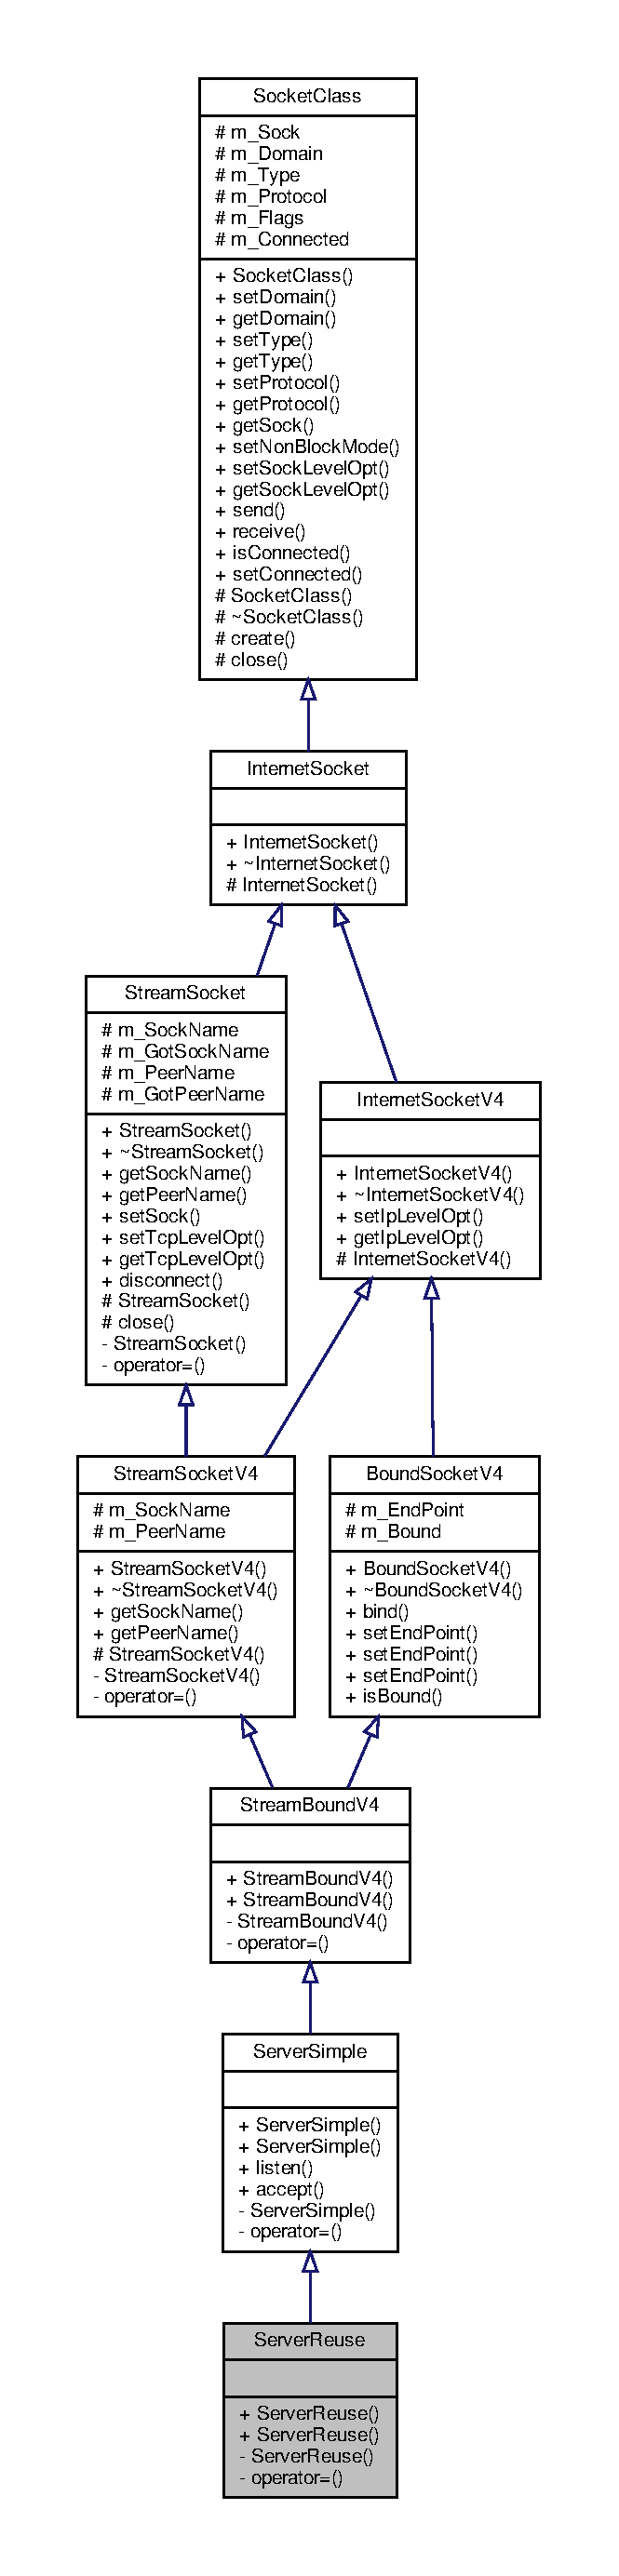
\includegraphics[height=550pt]{classServerReuse__inherit__graph}
\end{center}
\end{figure}
\subsection*{Public Member Functions}
\begin{DoxyCompactItemize}
\item 
\hyperlink{classServerReuse_ae875f0fb571e6df62a25b7371963e7bc}{Server\+Reuse} (short Port, in\+\_\+addr\+\_\+t Address=I\+N\+A\+D\+D\+R\+\_\+\+A\+NY)
\item 
\hyperlink{classServerReuse_abc7ad7021b9e7498488aeaca9712f378}{Server\+Reuse} (short Port, const char $\ast$Address)
\end{DoxyCompactItemize}
\subsection*{Private Member Functions}
\begin{DoxyCompactItemize}
\item 
\hyperlink{classServerReuse_af4d5bfd763f0411e025d86d5422abc74}{Server\+Reuse} (\hyperlink{classServerReuse}{Server\+Reuse} \&s)
\item 
\hyperlink{classServerReuse}{Server\+Reuse} \& \hyperlink{classServerReuse_a268c677f0e334f75d0d2151ab58b0131}{operator=} (\hyperlink{classServerReuse}{Server\+Reuse} \&s)
\end{DoxyCompactItemize}
\subsection*{Additional Inherited Members}


\subsection{Detailed Description}
T\+CP server socket with reuse local address ability. 

\subsection{Constructor \& Destructor Documentation}
\mbox{\Hypertarget{classServerReuse_ae875f0fb571e6df62a25b7371963e7bc}\label{classServerReuse_ae875f0fb571e6df62a25b7371963e7bc}} 
\index{Server\+Reuse@{Server\+Reuse}!Server\+Reuse@{Server\+Reuse}}
\index{Server\+Reuse@{Server\+Reuse}!Server\+Reuse@{Server\+Reuse}}
\subsubsection{\texorpdfstring{Server\+Reuse()}{ServerReuse()}\hspace{0.1cm}{\footnotesize\ttfamily [1/3]}}
{\footnotesize\ttfamily Server\+Reuse\+::\+Server\+Reuse (\begin{DoxyParamCaption}\item[{short}]{Port,  }\item[{in\+\_\+addr\+\_\+t}]{Address = {\ttfamily INADDR\+\_\+ANY} }\end{DoxyParamCaption})}

Constructor. 
\begin{DoxyParams}{Parameters}
{\em Port} & \+: port number for bind in network byte order. \\
\hline
{\em Address} & \+: I\+Pv4 address for bind in network byte order. \\
\hline
\end{DoxyParams}

\begin{DoxyExceptions}{Exceptions}
{\em Sock\+Exception.} & \\
\hline
\end{DoxyExceptions}
\mbox{\Hypertarget{classServerReuse_abc7ad7021b9e7498488aeaca9712f378}\label{classServerReuse_abc7ad7021b9e7498488aeaca9712f378}} 
\index{Server\+Reuse@{Server\+Reuse}!Server\+Reuse@{Server\+Reuse}}
\index{Server\+Reuse@{Server\+Reuse}!Server\+Reuse@{Server\+Reuse}}
\subsubsection{\texorpdfstring{Server\+Reuse()}{ServerReuse()}\hspace{0.1cm}{\footnotesize\ttfamily [2/3]}}
{\footnotesize\ttfamily Server\+Reuse\+::\+Server\+Reuse (\begin{DoxyParamCaption}\item[{short}]{Port,  }\item[{const char $\ast$}]{Address }\end{DoxyParamCaption})}

Constructor. 
\begin{DoxyParams}{Parameters}
{\em Port} & \+: port number for bind in network byte order. \\
\hline
{\em Address} & \+: I\+Pv4 address for bind in decimal dot notation. \\
\hline
\end{DoxyParams}

\begin{DoxyExceptions}{Exceptions}
{\em Sock\+Exception.} & \\
\hline
\end{DoxyExceptions}
\mbox{\Hypertarget{classServerReuse_af4d5bfd763f0411e025d86d5422abc74}\label{classServerReuse_af4d5bfd763f0411e025d86d5422abc74}} 
\index{Server\+Reuse@{Server\+Reuse}!Server\+Reuse@{Server\+Reuse}}
\index{Server\+Reuse@{Server\+Reuse}!Server\+Reuse@{Server\+Reuse}}
\subsubsection{\texorpdfstring{Server\+Reuse()}{ServerReuse()}\hspace{0.1cm}{\footnotesize\ttfamily [3/3]}}
{\footnotesize\ttfamily Server\+Reuse\+::\+Server\+Reuse (\begin{DoxyParamCaption}\item[{\hyperlink{classServerReuse}{Server\+Reuse} \&}]{s }\end{DoxyParamCaption})\hspace{0.3cm}{\ttfamily [private]}}

Copy constructor. Makes the class uncopyable. 

\subsection{Member Function Documentation}
\mbox{\Hypertarget{classServerReuse_a268c677f0e334f75d0d2151ab58b0131}\label{classServerReuse_a268c677f0e334f75d0d2151ab58b0131}} 
\index{Server\+Reuse@{Server\+Reuse}!operator=@{operator=}}
\index{operator=@{operator=}!Server\+Reuse@{Server\+Reuse}}
\subsubsection{\texorpdfstring{operator=()}{operator=()}}
{\footnotesize\ttfamily \hyperlink{classServerReuse}{Server\+Reuse}\& Server\+Reuse\+::operator= (\begin{DoxyParamCaption}\item[{\hyperlink{classServerReuse}{Server\+Reuse} \&}]{s }\end{DoxyParamCaption})\hspace{0.3cm}{\ttfamily [private]}}

Operator assign. Makes the class uncopyable. 

The documentation for this class was generated from the following files\+:\begin{DoxyCompactItemize}
\item 
\hyperlink{ServerReuse_8h}{Server\+Reuse.\+h}\item 
\hyperlink{ServerReuse_8cpp}{Server\+Reuse.\+cpp}\end{DoxyCompactItemize}

\hypertarget{classServerReuseV6}{}\section{Server\+Reuse\+V6 Class Reference}
\label{classServerReuseV6}\index{Server\+Reuse\+V6@{Server\+Reuse\+V6}}


T\+CP server socket with reuse local address ability.  




{\ttfamily \#include $<$Server\+Reuse\+V6.\+h$>$}



Inheritance diagram for Server\+Reuse\+V6\+:\nopagebreak
\begin{figure}[H]
\begin{center}
\leavevmode
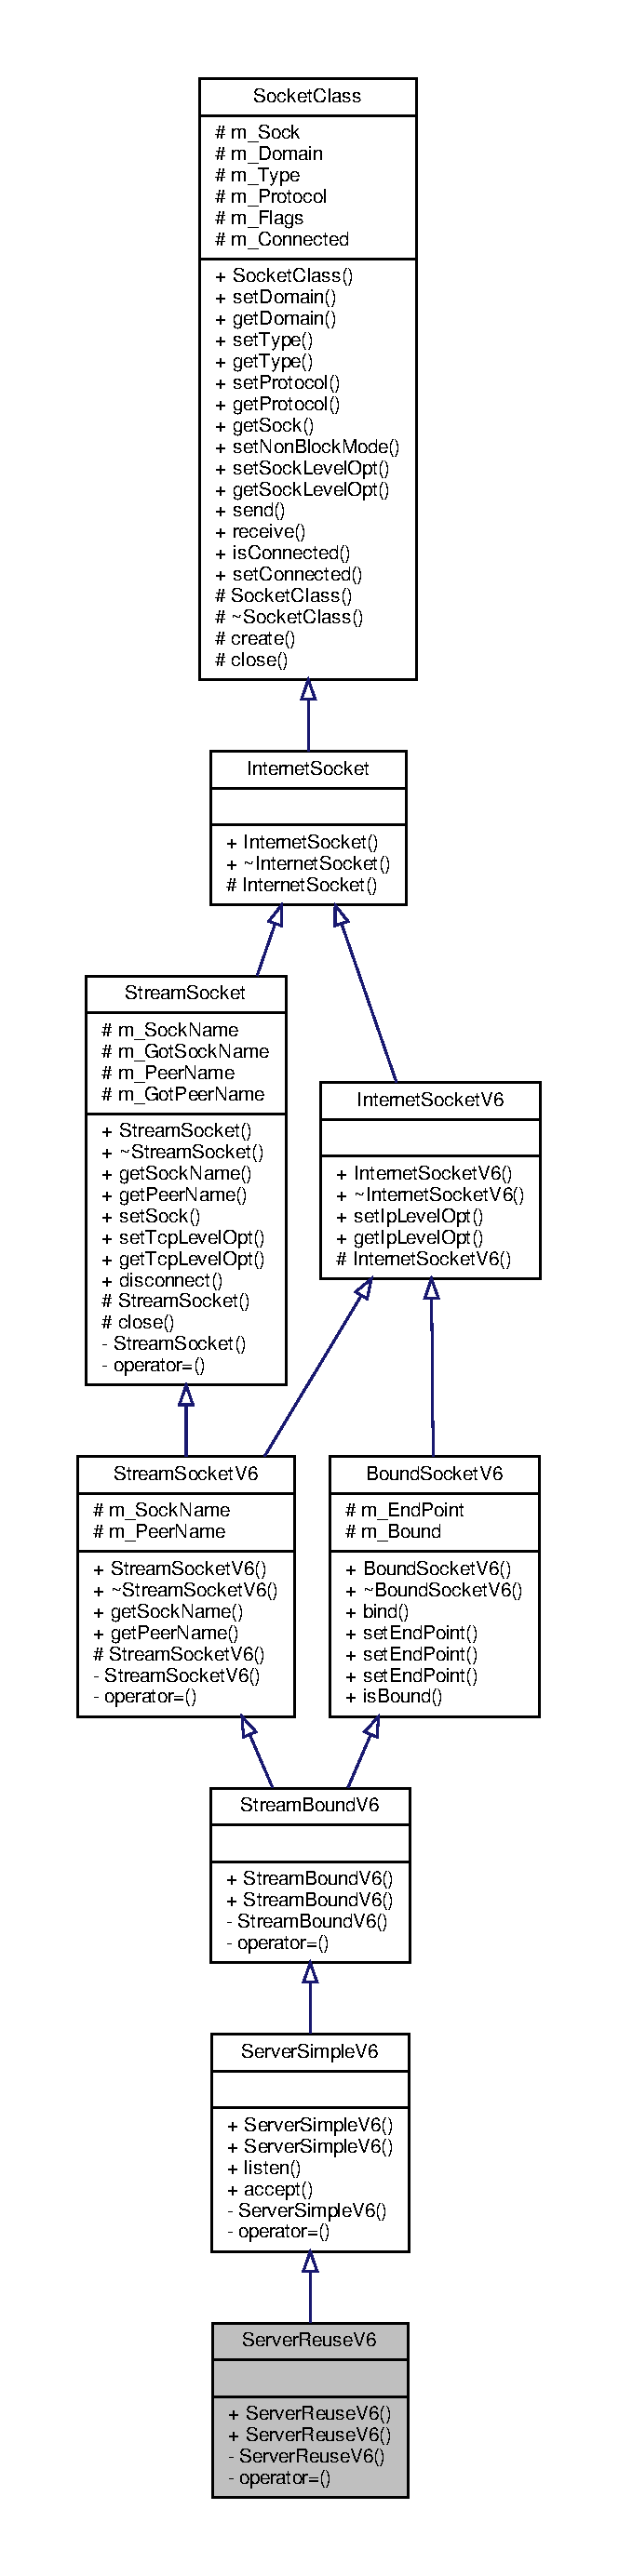
\includegraphics[height=550pt]{classServerReuseV6__inherit__graph}
\end{center}
\end{figure}
\subsection*{Public Member Functions}
\begin{DoxyCompactItemize}
\item 
\hyperlink{classServerReuseV6_ab18b2c131544cff19092e079cad65183}{Server\+Reuse\+V6} (short Port, in6\+\_\+addr Address=in6addr\+\_\+any)
\item 
\hyperlink{classServerReuseV6_aede672796d4fd33b27682fd6b0120ae2}{Server\+Reuse\+V6} (short Port, const char $\ast$Address)
\end{DoxyCompactItemize}
\subsection*{Private Member Functions}
\begin{DoxyCompactItemize}
\item 
\hyperlink{classServerReuseV6_a84ece67785e19d6ff31b002aa88d2bff}{Server\+Reuse\+V6} (\hyperlink{classServerReuseV6}{Server\+Reuse\+V6} \&s)
\item 
\hyperlink{classServerReuseV6}{Server\+Reuse\+V6} \& \hyperlink{classServerReuseV6_af517a336f3c8f9166ee1cc70e2e6a5f4}{operator=} (\hyperlink{classServerReuseV6}{Server\+Reuse\+V6} \&s)
\end{DoxyCompactItemize}
\subsection*{Additional Inherited Members}


\subsection{Detailed Description}
T\+CP server socket with reuse local address ability. 

\subsection{Constructor \& Destructor Documentation}
\mbox{\Hypertarget{classServerReuseV6_ab18b2c131544cff19092e079cad65183}\label{classServerReuseV6_ab18b2c131544cff19092e079cad65183}} 
\index{Server\+Reuse\+V6@{Server\+Reuse\+V6}!Server\+Reuse\+V6@{Server\+Reuse\+V6}}
\index{Server\+Reuse\+V6@{Server\+Reuse\+V6}!Server\+Reuse\+V6@{Server\+Reuse\+V6}}
\subsubsection{\texorpdfstring{Server\+Reuse\+V6()}{ServerReuseV6()}\hspace{0.1cm}{\footnotesize\ttfamily [1/3]}}
{\footnotesize\ttfamily Server\+Reuse\+V6\+::\+Server\+Reuse\+V6 (\begin{DoxyParamCaption}\item[{short}]{Port,  }\item[{in6\+\_\+addr}]{Address = {\ttfamily in6addr\+\_\+any} }\end{DoxyParamCaption})}

Constructor. 
\begin{DoxyParams}{Parameters}
{\em Port} & \+: port number for bind in network byte order. \\
\hline
{\em Address} & \+: I\+Pv6 address for bind in network byte order. \\
\hline
\end{DoxyParams}

\begin{DoxyExceptions}{Exceptions}
{\em Sock\+Exception.} & \\
\hline
\end{DoxyExceptions}
\mbox{\Hypertarget{classServerReuseV6_aede672796d4fd33b27682fd6b0120ae2}\label{classServerReuseV6_aede672796d4fd33b27682fd6b0120ae2}} 
\index{Server\+Reuse\+V6@{Server\+Reuse\+V6}!Server\+Reuse\+V6@{Server\+Reuse\+V6}}
\index{Server\+Reuse\+V6@{Server\+Reuse\+V6}!Server\+Reuse\+V6@{Server\+Reuse\+V6}}
\subsubsection{\texorpdfstring{Server\+Reuse\+V6()}{ServerReuseV6()}\hspace{0.1cm}{\footnotesize\ttfamily [2/3]}}
{\footnotesize\ttfamily Server\+Reuse\+V6\+::\+Server\+Reuse\+V6 (\begin{DoxyParamCaption}\item[{short}]{Port,  }\item[{const char $\ast$}]{Address }\end{DoxyParamCaption})}

Constructor. 
\begin{DoxyParams}{Parameters}
{\em Port} & \+: port number for bind in network byte order. \\
\hline
{\em Address} & \+: I\+Pv6 address for bind in textual notation. \\
\hline
\end{DoxyParams}

\begin{DoxyExceptions}{Exceptions}
{\em Sock\+Exception.} & \\
\hline
\end{DoxyExceptions}
\mbox{\Hypertarget{classServerReuseV6_a84ece67785e19d6ff31b002aa88d2bff}\label{classServerReuseV6_a84ece67785e19d6ff31b002aa88d2bff}} 
\index{Server\+Reuse\+V6@{Server\+Reuse\+V6}!Server\+Reuse\+V6@{Server\+Reuse\+V6}}
\index{Server\+Reuse\+V6@{Server\+Reuse\+V6}!Server\+Reuse\+V6@{Server\+Reuse\+V6}}
\subsubsection{\texorpdfstring{Server\+Reuse\+V6()}{ServerReuseV6()}\hspace{0.1cm}{\footnotesize\ttfamily [3/3]}}
{\footnotesize\ttfamily Server\+Reuse\+V6\+::\+Server\+Reuse\+V6 (\begin{DoxyParamCaption}\item[{\hyperlink{classServerReuseV6}{Server\+Reuse\+V6} \&}]{s }\end{DoxyParamCaption})\hspace{0.3cm}{\ttfamily [private]}}

Copy constructor. Makes the class uncopyable. 

\subsection{Member Function Documentation}
\mbox{\Hypertarget{classServerReuseV6_af517a336f3c8f9166ee1cc70e2e6a5f4}\label{classServerReuseV6_af517a336f3c8f9166ee1cc70e2e6a5f4}} 
\index{Server\+Reuse\+V6@{Server\+Reuse\+V6}!operator=@{operator=}}
\index{operator=@{operator=}!Server\+Reuse\+V6@{Server\+Reuse\+V6}}
\subsubsection{\texorpdfstring{operator=()}{operator=()}}
{\footnotesize\ttfamily \hyperlink{classServerReuseV6}{Server\+Reuse\+V6}\& Server\+Reuse\+V6\+::operator= (\begin{DoxyParamCaption}\item[{\hyperlink{classServerReuseV6}{Server\+Reuse\+V6} \&}]{s }\end{DoxyParamCaption})\hspace{0.3cm}{\ttfamily [private]}}

Operator assign. Makes the class uncopyable. 

The documentation for this class was generated from the following files\+:\begin{DoxyCompactItemize}
\item 
\hyperlink{ServerReuseV6_8h}{Server\+Reuse\+V6.\+h}\item 
\hyperlink{ServerReuseV6_8cpp}{Server\+Reuse\+V6.\+cpp}\end{DoxyCompactItemize}

\hypertarget{classServerSimple}{}\section{Server\+Simple Class Reference}
\label{classServerSimple}\index{Server\+Simple@{Server\+Simple}}


T\+CP server socket.  




{\ttfamily \#include $<$Server\+Simple.\+h$>$}



Inheritance diagram for Server\+Simple\+:\nopagebreak
\begin{figure}[H]
\begin{center}
\leavevmode
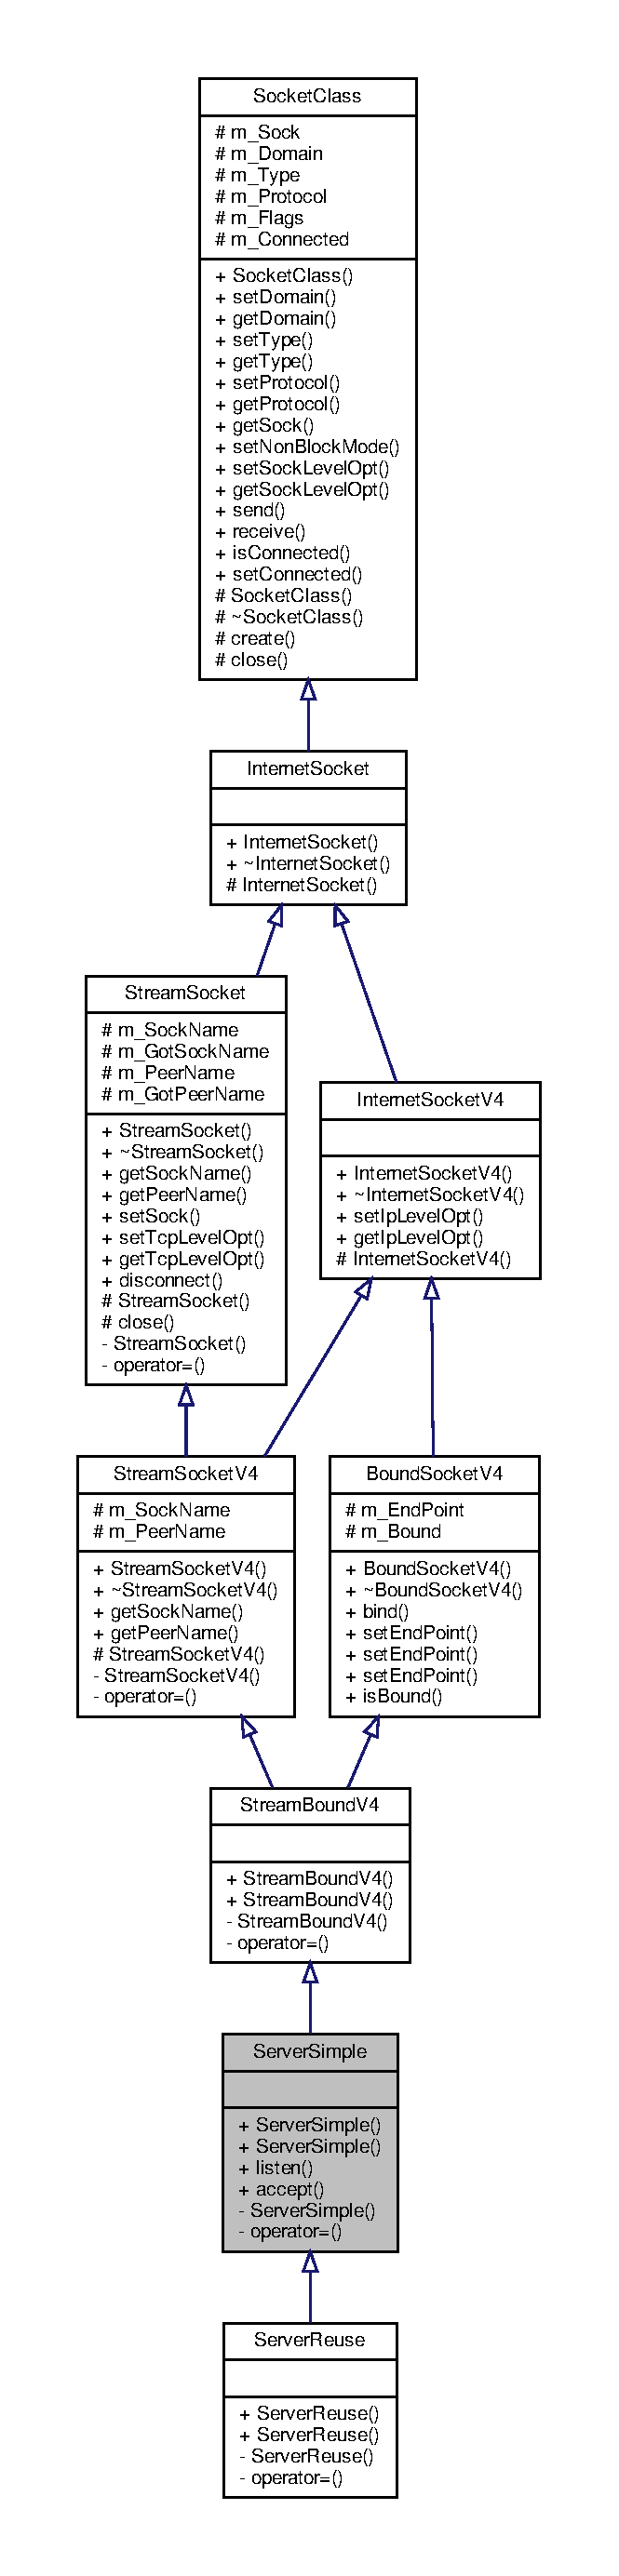
\includegraphics[height=550pt]{classServerSimple__inherit__graph}
\end{center}
\end{figure}
\subsection*{Public Member Functions}
\begin{DoxyCompactItemize}
\item 
\hyperlink{classServerSimple_a9ed49ad0f3ebaaae208886c472d06827}{Server\+Simple} (short Port, in\+\_\+addr\+\_\+t Address=I\+N\+A\+D\+D\+R\+\_\+\+A\+NY, bool Late\+Bind=false)
\item 
\hyperlink{classServerSimple_a47713f4385917c592b2db4236b27e20e}{Server\+Simple} (short Port, const char $\ast$Address, bool Late\+Bind=false)
\item 
virtual void \hyperlink{classServerSimple_ae2c87189faf4d3b0c87e160bd561be05}{listen} (int Backlog=5)
\item 
virtual \hyperlink{classStreamSocketV4}{Stream\+Socket\+V4} $\ast$ \hyperlink{classServerSimple_ad1494d88a28fdb9c392ed9b03172fdfd}{accept} ()
\end{DoxyCompactItemize}
\subsection*{Private Member Functions}
\begin{DoxyCompactItemize}
\item 
\hyperlink{classServerSimple_a8e89675d8a51130655cf8060d203c287}{Server\+Simple} (\hyperlink{classServerSimple}{Server\+Simple} \&s)
\item 
\hyperlink{classServerSimple}{Server\+Simple} \& \hyperlink{classServerSimple_a2c144e6e1b4a58b4edd838db998f5903}{operator=} (\hyperlink{classServerSimple}{Server\+Simple} \&s)
\end{DoxyCompactItemize}
\subsection*{Additional Inherited Members}


\subsection{Detailed Description}
T\+CP server socket. 

\subsection{Constructor \& Destructor Documentation}
\mbox{\Hypertarget{classServerSimple_a9ed49ad0f3ebaaae208886c472d06827}\label{classServerSimple_a9ed49ad0f3ebaaae208886c472d06827}} 
\index{Server\+Simple@{Server\+Simple}!Server\+Simple@{Server\+Simple}}
\index{Server\+Simple@{Server\+Simple}!Server\+Simple@{Server\+Simple}}
\subsubsection{\texorpdfstring{Server\+Simple()}{ServerSimple()}\hspace{0.1cm}{\footnotesize\ttfamily [1/3]}}
{\footnotesize\ttfamily Server\+Simple\+::\+Server\+Simple (\begin{DoxyParamCaption}\item[{short}]{Port,  }\item[{in\+\_\+addr\+\_\+t}]{Address = {\ttfamily INADDR\+\_\+ANY},  }\item[{bool}]{Late\+Bind = {\ttfamily false} }\end{DoxyParamCaption})\hspace{0.3cm}{\ttfamily [inline]}}

Constructor. 
\begin{DoxyParams}{Parameters}
{\em Port} & \+: port number for bind in network byte order. \\
\hline
{\em Address} & \+: address for bind in network byte order. \\
\hline
{\em Late\+Bind} & \+: do bind now or later according to bind method call. \\
\hline
\end{DoxyParams}

\begin{DoxyExceptions}{Exceptions}
{\em Sock\+Exception.} & \\
\hline
\end{DoxyExceptions}
\mbox{\Hypertarget{classServerSimple_a47713f4385917c592b2db4236b27e20e}\label{classServerSimple_a47713f4385917c592b2db4236b27e20e}} 
\index{Server\+Simple@{Server\+Simple}!Server\+Simple@{Server\+Simple}}
\index{Server\+Simple@{Server\+Simple}!Server\+Simple@{Server\+Simple}}
\subsubsection{\texorpdfstring{Server\+Simple()}{ServerSimple()}\hspace{0.1cm}{\footnotesize\ttfamily [2/3]}}
{\footnotesize\ttfamily Server\+Simple\+::\+Server\+Simple (\begin{DoxyParamCaption}\item[{short}]{Port,  }\item[{const char $\ast$}]{Address,  }\item[{bool}]{Late\+Bind = {\ttfamily false} }\end{DoxyParamCaption})\hspace{0.3cm}{\ttfamily [inline]}}

Constructor. 
\begin{DoxyParams}{Parameters}
{\em Port} & \+: port number for bind in network byte order. \\
\hline
{\em Address} & \+: I\+Pv4 address for bind in decimal dot notation. \\
\hline
{\em Late\+Bind} & \+: do bind now or later according to bind method call. \\
\hline
\end{DoxyParams}

\begin{DoxyExceptions}{Exceptions}
{\em Sock\+Exception.} & \\
\hline
\end{DoxyExceptions}
\mbox{\Hypertarget{classServerSimple_a8e89675d8a51130655cf8060d203c287}\label{classServerSimple_a8e89675d8a51130655cf8060d203c287}} 
\index{Server\+Simple@{Server\+Simple}!Server\+Simple@{Server\+Simple}}
\index{Server\+Simple@{Server\+Simple}!Server\+Simple@{Server\+Simple}}
\subsubsection{\texorpdfstring{Server\+Simple()}{ServerSimple()}\hspace{0.1cm}{\footnotesize\ttfamily [3/3]}}
{\footnotesize\ttfamily Server\+Simple\+::\+Server\+Simple (\begin{DoxyParamCaption}\item[{\hyperlink{classServerSimple}{Server\+Simple} \&}]{s }\end{DoxyParamCaption})\hspace{0.3cm}{\ttfamily [private]}}

Copy constructor. Makes the class uncopyable. 

\subsection{Member Function Documentation}
\mbox{\Hypertarget{classServerSimple_ad1494d88a28fdb9c392ed9b03172fdfd}\label{classServerSimple_ad1494d88a28fdb9c392ed9b03172fdfd}} 
\index{Server\+Simple@{Server\+Simple}!accept@{accept}}
\index{accept@{accept}!Server\+Simple@{Server\+Simple}}
\subsubsection{\texorpdfstring{accept()}{accept()}}
{\footnotesize\ttfamily \hyperlink{classStreamSocketV4}{Stream\+Socket\+V4} $\ast$ Server\+Simple\+::accept (\begin{DoxyParamCaption}{ }\end{DoxyParamCaption})\hspace{0.3cm}{\ttfamily [virtual]}}

Accept connection request. \begin{DoxyReturn}{Returns}
\hyperlink{classStreamSocketV4}{Stream\+Socket\+V4} pointer representing local connection endpoint. 
\end{DoxyReturn}

\begin{DoxyExceptions}{Exceptions}
{\em Sock\+Exception.} & \\
\hline
\end{DoxyExceptions}
\mbox{\Hypertarget{classServerSimple_ae2c87189faf4d3b0c87e160bd561be05}\label{classServerSimple_ae2c87189faf4d3b0c87e160bd561be05}} 
\index{Server\+Simple@{Server\+Simple}!listen@{listen}}
\index{listen@{listen}!Server\+Simple@{Server\+Simple}}
\subsubsection{\texorpdfstring{listen()}{listen()}}
{\footnotesize\ttfamily void Server\+Simple\+::listen (\begin{DoxyParamCaption}\item[{int}]{Backlog = {\ttfamily 5} }\end{DoxyParamCaption})\hspace{0.3cm}{\ttfamily [virtual]}}

Listen for input connections. 
\begin{DoxyParams}{Parameters}
{\em Backlog} & \+: number of simultaneously held connection requests. \\
\hline
\end{DoxyParams}

\begin{DoxyExceptions}{Exceptions}
{\em Sock\+Exception.} & \\
\hline
\end{DoxyExceptions}
\mbox{\Hypertarget{classServerSimple_a2c144e6e1b4a58b4edd838db998f5903}\label{classServerSimple_a2c144e6e1b4a58b4edd838db998f5903}} 
\index{Server\+Simple@{Server\+Simple}!operator=@{operator=}}
\index{operator=@{operator=}!Server\+Simple@{Server\+Simple}}
\subsubsection{\texorpdfstring{operator=()}{operator=()}}
{\footnotesize\ttfamily \hyperlink{classServerSimple}{Server\+Simple}\& Server\+Simple\+::operator= (\begin{DoxyParamCaption}\item[{\hyperlink{classServerSimple}{Server\+Simple} \&}]{s }\end{DoxyParamCaption})\hspace{0.3cm}{\ttfamily [private]}}

Operator assign. Makes the class uncopyable. 

The documentation for this class was generated from the following files\+:\begin{DoxyCompactItemize}
\item 
\hyperlink{ServerSimple_8h}{Server\+Simple.\+h}\item 
\hyperlink{ServerSimple_8cpp}{Server\+Simple.\+cpp}\end{DoxyCompactItemize}

\hypertarget{classServerSimpleV6}{}\section{Server\+Simple\+V6 Class Reference}
\label{classServerSimpleV6}\index{Server\+Simple\+V6@{Server\+Simple\+V6}}


T\+CP server socket.  




{\ttfamily \#include $<$Server\+Simple\+V6.\+h$>$}



Inheritance diagram for Server\+Simple\+V6\+:\nopagebreak
\begin{figure}[H]
\begin{center}
\leavevmode
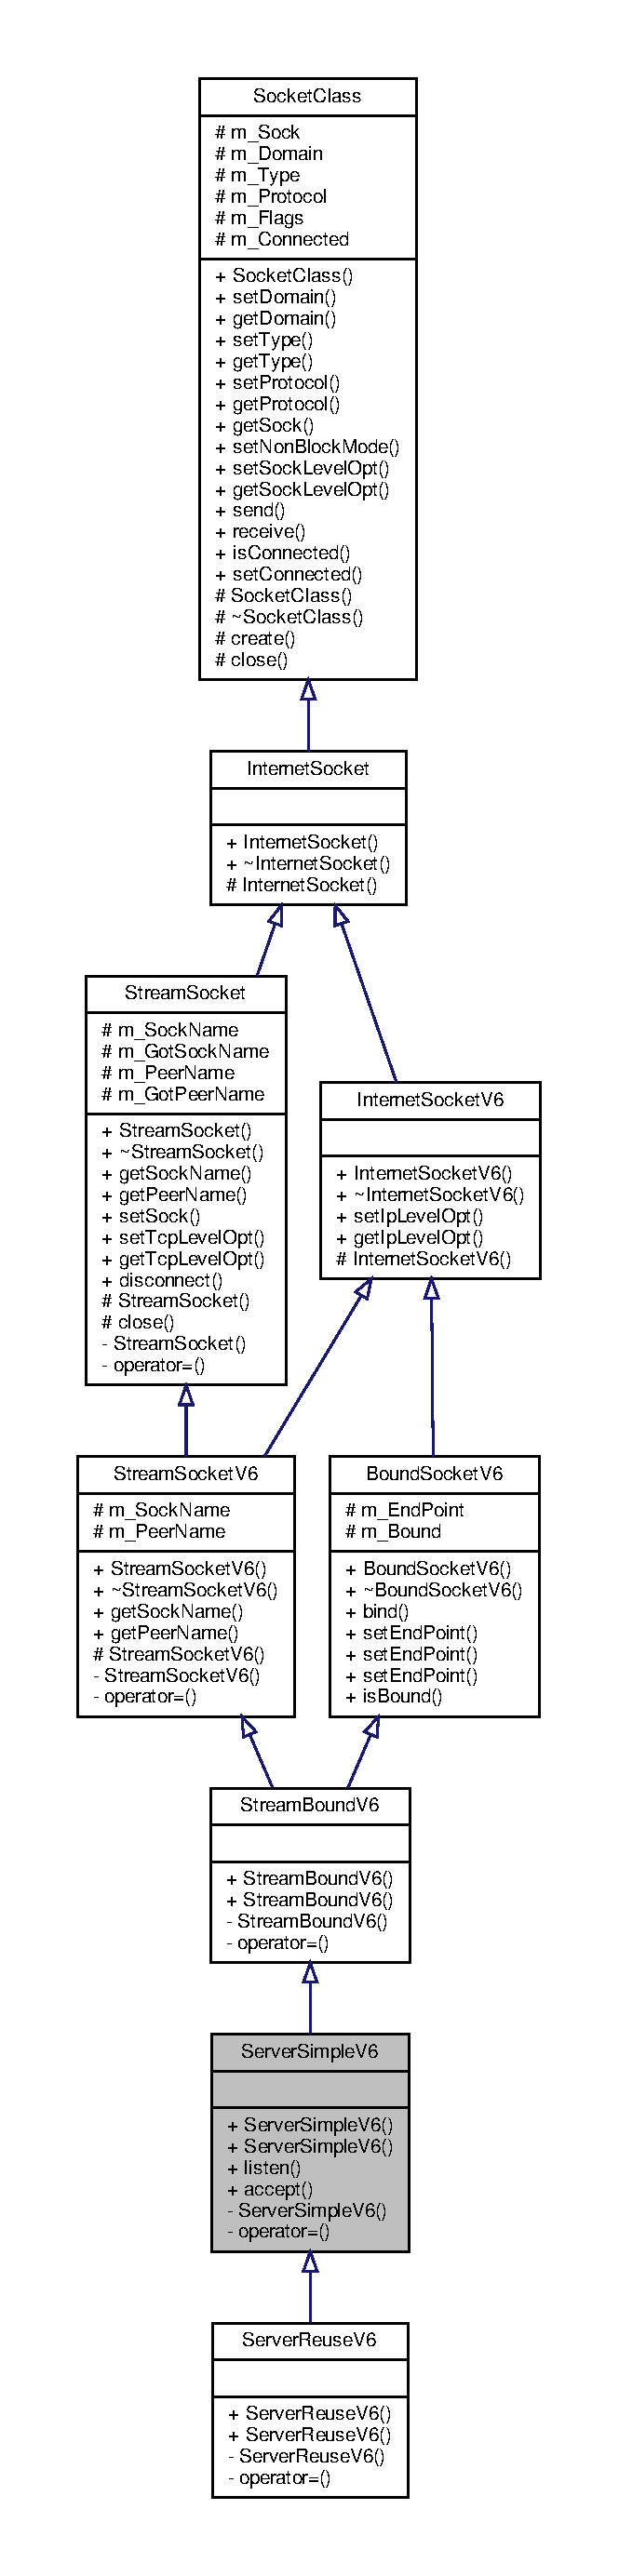
\includegraphics[height=550pt]{classServerSimpleV6__inherit__graph}
\end{center}
\end{figure}
\subsection*{Public Member Functions}
\begin{DoxyCompactItemize}
\item 
\hyperlink{classServerSimpleV6_a6efa36464d2455c565a297c1775bd822}{Server\+Simple\+V6} (short Port, in6\+\_\+addr Address=in6addr\+\_\+any, bool Late\+Bind=false)
\item 
\hyperlink{classServerSimpleV6_afa86ebe69d65a75dc40bd98287887618}{Server\+Simple\+V6} (short Port, const char $\ast$Address, bool Late\+Bind=false)
\item 
virtual void \hyperlink{classServerSimpleV6_a4ea81562c4f7536ab7fe46ecb8e052d9}{listen} (int Backlog=5)
\item 
virtual \hyperlink{classStreamSocketV6}{Stream\+Socket\+V6} $\ast$ \hyperlink{classServerSimpleV6_aae8c9ed7be029ad52254b0ea6540d8f0}{accept} ()
\end{DoxyCompactItemize}
\subsection*{Private Member Functions}
\begin{DoxyCompactItemize}
\item 
\hyperlink{classServerSimpleV6_a1ced02f63d5868928d3f3935ecbecb36}{Server\+Simple\+V6} (\hyperlink{classServerSimpleV6}{Server\+Simple\+V6} \&s)
\item 
\hyperlink{classServerSimpleV6}{Server\+Simple\+V6} \& \hyperlink{classServerSimpleV6_ac40d7415b445df1fdd8b53653dace8ff}{operator=} (\hyperlink{classServerSimpleV6}{Server\+Simple\+V6} \&s)
\end{DoxyCompactItemize}
\subsection*{Additional Inherited Members}


\subsection{Detailed Description}
T\+CP server socket. 

\subsection{Constructor \& Destructor Documentation}
\mbox{\Hypertarget{classServerSimpleV6_a6efa36464d2455c565a297c1775bd822}\label{classServerSimpleV6_a6efa36464d2455c565a297c1775bd822}} 
\index{Server\+Simple\+V6@{Server\+Simple\+V6}!Server\+Simple\+V6@{Server\+Simple\+V6}}
\index{Server\+Simple\+V6@{Server\+Simple\+V6}!Server\+Simple\+V6@{Server\+Simple\+V6}}
\subsubsection{\texorpdfstring{Server\+Simple\+V6()}{ServerSimpleV6()}\hspace{0.1cm}{\footnotesize\ttfamily [1/3]}}
{\footnotesize\ttfamily Server\+Simple\+V6\+::\+Server\+Simple\+V6 (\begin{DoxyParamCaption}\item[{short}]{Port,  }\item[{in6\+\_\+addr}]{Address = {\ttfamily in6addr\+\_\+any},  }\item[{bool}]{Late\+Bind = {\ttfamily false} }\end{DoxyParamCaption})\hspace{0.3cm}{\ttfamily [inline]}}

Constructor. 
\begin{DoxyParams}{Parameters}
{\em Port} & \+: port number for bind in network byte order. \\
\hline
{\em Address} & \+: I\+Pv6 address for bind in network byte order. \\
\hline
{\em Late\+Bind} & \+: do bind now or later according to bind method call. \\
\hline
\end{DoxyParams}

\begin{DoxyExceptions}{Exceptions}
{\em Sock\+Exception.} & \\
\hline
\end{DoxyExceptions}
\mbox{\Hypertarget{classServerSimpleV6_afa86ebe69d65a75dc40bd98287887618}\label{classServerSimpleV6_afa86ebe69d65a75dc40bd98287887618}} 
\index{Server\+Simple\+V6@{Server\+Simple\+V6}!Server\+Simple\+V6@{Server\+Simple\+V6}}
\index{Server\+Simple\+V6@{Server\+Simple\+V6}!Server\+Simple\+V6@{Server\+Simple\+V6}}
\subsubsection{\texorpdfstring{Server\+Simple\+V6()}{ServerSimpleV6()}\hspace{0.1cm}{\footnotesize\ttfamily [2/3]}}
{\footnotesize\ttfamily Server\+Simple\+V6\+::\+Server\+Simple\+V6 (\begin{DoxyParamCaption}\item[{short}]{Port,  }\item[{const char $\ast$}]{Address,  }\item[{bool}]{Late\+Bind = {\ttfamily false} }\end{DoxyParamCaption})\hspace{0.3cm}{\ttfamily [inline]}}

Constructor. 
\begin{DoxyParams}{Parameters}
{\em Port} & \+: port number for bind in network byte order. \\
\hline
{\em Address} & \+: I\+Pv6 address for bind in textual notation. \\
\hline
{\em Late\+Bind} & \+: do bind now or later according to bind method call. \\
\hline
\end{DoxyParams}

\begin{DoxyExceptions}{Exceptions}
{\em Sock\+Exception.} & \\
\hline
\end{DoxyExceptions}
\mbox{\Hypertarget{classServerSimpleV6_a1ced02f63d5868928d3f3935ecbecb36}\label{classServerSimpleV6_a1ced02f63d5868928d3f3935ecbecb36}} 
\index{Server\+Simple\+V6@{Server\+Simple\+V6}!Server\+Simple\+V6@{Server\+Simple\+V6}}
\index{Server\+Simple\+V6@{Server\+Simple\+V6}!Server\+Simple\+V6@{Server\+Simple\+V6}}
\subsubsection{\texorpdfstring{Server\+Simple\+V6()}{ServerSimpleV6()}\hspace{0.1cm}{\footnotesize\ttfamily [3/3]}}
{\footnotesize\ttfamily Server\+Simple\+V6\+::\+Server\+Simple\+V6 (\begin{DoxyParamCaption}\item[{\hyperlink{classServerSimpleV6}{Server\+Simple\+V6} \&}]{s }\end{DoxyParamCaption})\hspace{0.3cm}{\ttfamily [private]}}

Copy constructor. Makes the class uncopyable. 

\subsection{Member Function Documentation}
\mbox{\Hypertarget{classServerSimpleV6_aae8c9ed7be029ad52254b0ea6540d8f0}\label{classServerSimpleV6_aae8c9ed7be029ad52254b0ea6540d8f0}} 
\index{Server\+Simple\+V6@{Server\+Simple\+V6}!accept@{accept}}
\index{accept@{accept}!Server\+Simple\+V6@{Server\+Simple\+V6}}
\subsubsection{\texorpdfstring{accept()}{accept()}}
{\footnotesize\ttfamily \hyperlink{classStreamSocketV6}{Stream\+Socket\+V6} $\ast$ Server\+Simple\+V6\+::accept (\begin{DoxyParamCaption}{ }\end{DoxyParamCaption})\hspace{0.3cm}{\ttfamily [virtual]}}

Accept connection request. \begin{DoxyReturn}{Returns}
\hyperlink{classStreamSocketV6}{Stream\+Socket\+V6} pointer representing local connection endpoint. 
\end{DoxyReturn}

\begin{DoxyExceptions}{Exceptions}
{\em Sock\+Exception.} & \\
\hline
\end{DoxyExceptions}
\mbox{\Hypertarget{classServerSimpleV6_a4ea81562c4f7536ab7fe46ecb8e052d9}\label{classServerSimpleV6_a4ea81562c4f7536ab7fe46ecb8e052d9}} 
\index{Server\+Simple\+V6@{Server\+Simple\+V6}!listen@{listen}}
\index{listen@{listen}!Server\+Simple\+V6@{Server\+Simple\+V6}}
\subsubsection{\texorpdfstring{listen()}{listen()}}
{\footnotesize\ttfamily void Server\+Simple\+V6\+::listen (\begin{DoxyParamCaption}\item[{int}]{Backlog = {\ttfamily 5} }\end{DoxyParamCaption})\hspace{0.3cm}{\ttfamily [virtual]}}

Listen for input connections. 
\begin{DoxyParams}{Parameters}
{\em Backlog} & \+: number of simultaneously held connection requests. \\
\hline
\end{DoxyParams}

\begin{DoxyExceptions}{Exceptions}
{\em Sock\+Exception.} & \\
\hline
\end{DoxyExceptions}
\mbox{\Hypertarget{classServerSimpleV6_ac40d7415b445df1fdd8b53653dace8ff}\label{classServerSimpleV6_ac40d7415b445df1fdd8b53653dace8ff}} 
\index{Server\+Simple\+V6@{Server\+Simple\+V6}!operator=@{operator=}}
\index{operator=@{operator=}!Server\+Simple\+V6@{Server\+Simple\+V6}}
\subsubsection{\texorpdfstring{operator=()}{operator=()}}
{\footnotesize\ttfamily \hyperlink{classServerSimpleV6}{Server\+Simple\+V6}\& Server\+Simple\+V6\+::operator= (\begin{DoxyParamCaption}\item[{\hyperlink{classServerSimpleV6}{Server\+Simple\+V6} \&}]{s }\end{DoxyParamCaption})\hspace{0.3cm}{\ttfamily [private]}}

Operator assign. Makes the class uncopyable. 

The documentation for this class was generated from the following files\+:\begin{DoxyCompactItemize}
\item 
\hyperlink{ServerSimpleV6_8h}{Server\+Simple\+V6.\+h}\item 
\hyperlink{ServerSimpleV6_8cpp}{Server\+Simple\+V6.\+cpp}\end{DoxyCompactItemize}

\hypertarget{classSocketClass}{}\section{Socket\+Class Class Reference}
\label{classSocketClass}\index{Socket\+Class@{Socket\+Class}}


{\ttfamily \#include $<$Socket\+Class.\+h$>$}



Inheritance diagram for Socket\+Class\+:\nopagebreak
\begin{figure}[H]
\begin{center}
\leavevmode
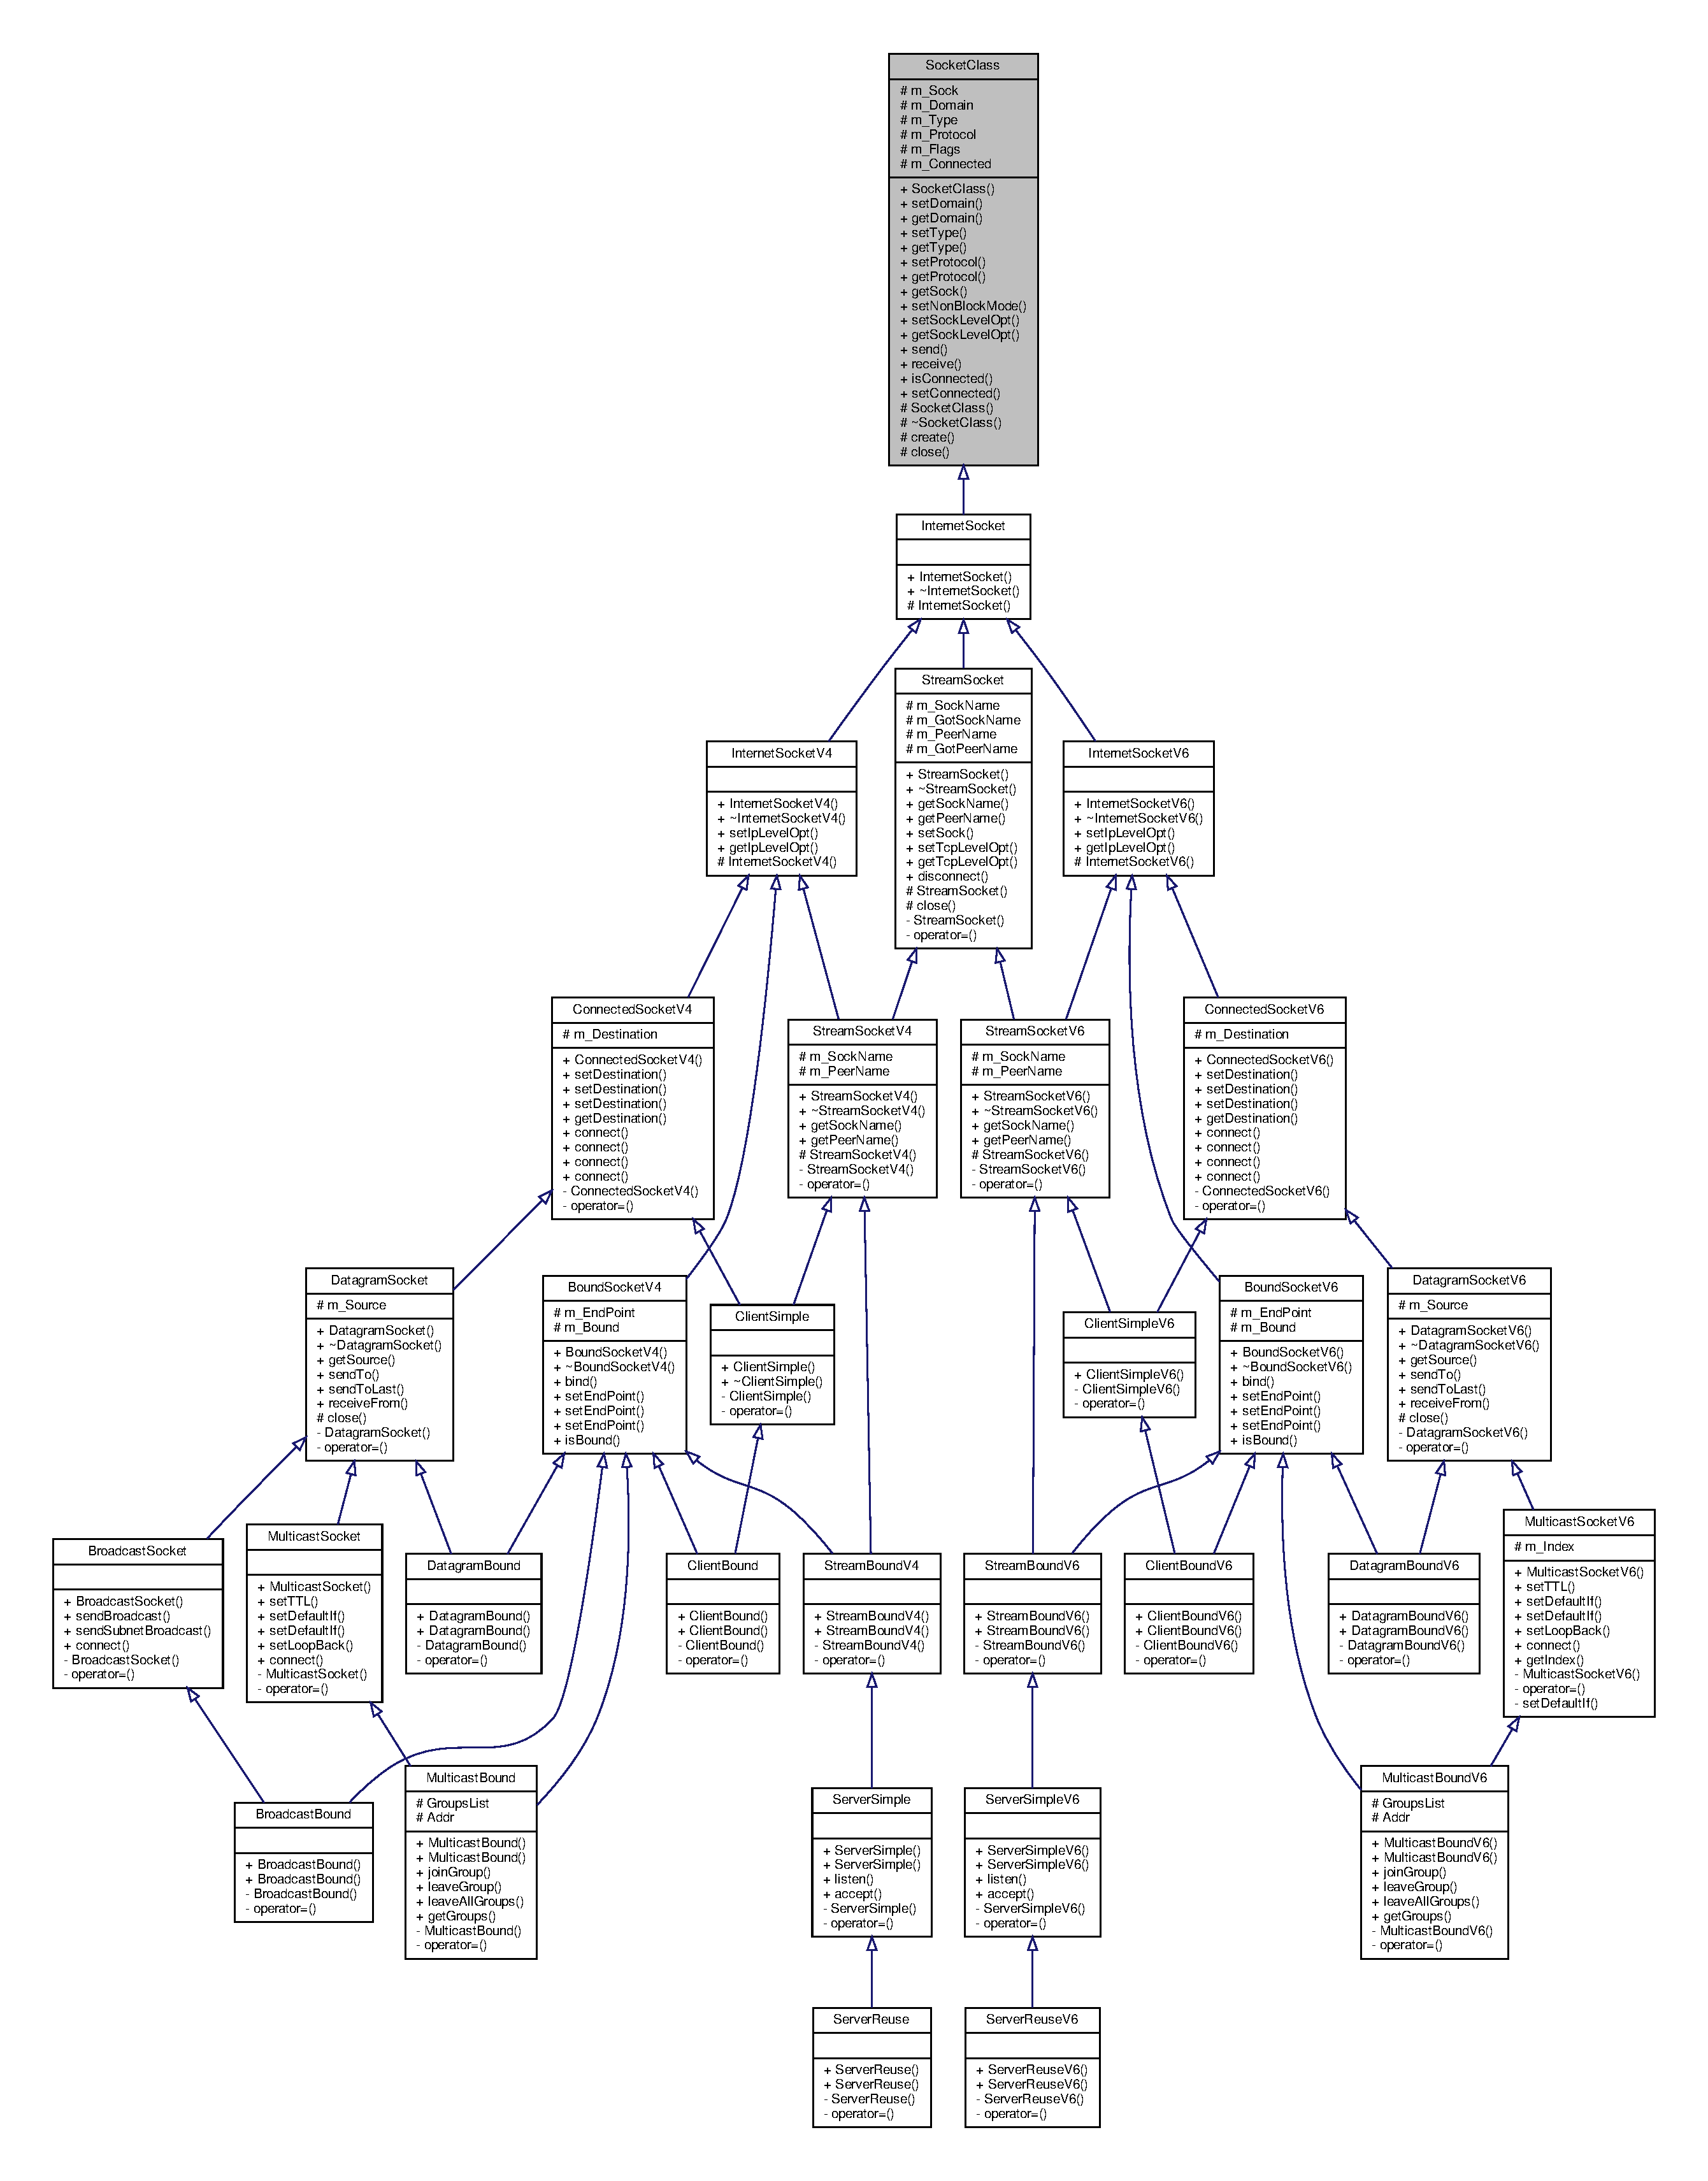
\includegraphics[width=350pt]{classSocketClass__inherit__graph}
\end{center}
\end{figure}
\subsection*{Public Types}
\begin{DoxyCompactItemize}
\item 
enum \hyperlink{classSocketClass_ac940413abaa7328db8518a9f121babb6}{Sock\+Domain} \{ \newline
\hyperlink{classSocketClass_ac940413abaa7328db8518a9f121babb6aa9ec2a4d642c47813fe90f362603f1c4}{N\+O\+\_\+\+D\+O\+M\+A\+IN} = A\+F\+\_\+\+U\+N\+S\+P\+EC, 
\hyperlink{classSocketClass_ac940413abaa7328db8518a9f121babb6ab92d1dfedf24d12d2b9f58b8d3a85be5}{U\+N\+I\+X\+\_\+\+D\+O\+M\+A\+IN} = A\+F\+\_\+\+U\+N\+IX, 
\hyperlink{classSocketClass_ac940413abaa7328db8518a9f121babb6a2cc4ca83a7b48c990a3454120b6af0b4}{I\+N\+T\+E\+R\+N\+E\+T\+\_\+\+D\+O\+M\+A\+IN} = A\+F\+\_\+\+I\+N\+ET, 
\hyperlink{classSocketClass_ac940413abaa7328db8518a9f121babb6a8b4768bb03b79d7cd9b73eb5e75584d4}{I\+P\+X\+\_\+\+D\+O\+M\+A\+IN} = A\+F\+\_\+\+I\+PX, 
\newline
\hyperlink{classSocketClass_ac940413abaa7328db8518a9f121babb6a531a739bc633378bafd6b248f2d21567}{R\+O\+U\+T\+I\+N\+G\+\_\+\+D\+O\+M\+A\+IN} = A\+F\+\_\+\+R\+O\+U\+TE, 
\hyperlink{classSocketClass_ac940413abaa7328db8518a9f121babb6abe0484126572a8667d5290faba923bf3}{I\+N\+E\+T6\+\_\+\+D\+O\+M\+A\+IN} = A\+F\+\_\+\+I\+N\+E\+T6
 \}
\item 
enum \hyperlink{classSocketClass_a2182dd9fee09459fabb99e6ae717f595}{Sock\+Type} \{ \hyperlink{classSocketClass_a2182dd9fee09459fabb99e6ae717f595a8c7f955ea5b71498ff1d469345d813ad}{N\+O\+\_\+\+T\+Y\+PE} = -\/1, 
\hyperlink{classSocketClass_a2182dd9fee09459fabb99e6ae717f595a804fd19ca5ff4bfaf2564830bb3ea82b}{U\+D\+P\+\_\+\+S\+O\+CK} = S\+O\+C\+K\+\_\+\+D\+G\+R\+AM, 
\hyperlink{classSocketClass_a2182dd9fee09459fabb99e6ae717f595a76163824c40569e670cd455185cf46e9}{T\+C\+P\+\_\+\+S\+O\+CK} = S\+O\+C\+K\+\_\+\+S\+T\+R\+E\+AM, 
\hyperlink{classSocketClass_a2182dd9fee09459fabb99e6ae717f595a2e14668dd087d168ed5f5f837c1b2ff1}{R\+A\+W\+\_\+\+S\+O\+CK} = S\+O\+C\+K\+\_\+\+R\+AW
 \}\begin{DoxyCompactList}\small\item\em Socket type enumeration. \end{DoxyCompactList}
\end{DoxyCompactItemize}
\subsection*{Public Member Functions}
\begin{DoxyCompactItemize}
\item 
\hyperlink{classSocketClass_a6a12a3d812e5063bf9f432fdf81ad059}{Socket\+Class} (\hyperlink{classSocketClass_ac940413abaa7328db8518a9f121babb6}{Sock\+Domain} domain=\hyperlink{classSocketClass_ac940413abaa7328db8518a9f121babb6aa9ec2a4d642c47813fe90f362603f1c4}{N\+O\+\_\+\+D\+O\+M\+A\+IN}, \hyperlink{classSocketClass_a2182dd9fee09459fabb99e6ae717f595}{Sock\+Type} type=\hyperlink{classSocketClass_a2182dd9fee09459fabb99e6ae717f595a8c7f955ea5b71498ff1d469345d813ad}{N\+O\+\_\+\+T\+Y\+PE}, int protocol=0)
\item 
void \hyperlink{classSocketClass_af1b60fc7b1b9fb0ce1ec999f65ca2bf0}{set\+Domain} (\hyperlink{classSocketClass_ac940413abaa7328db8518a9f121babb6}{Sock\+Domain} Domain)
\item 
\hyperlink{classSocketClass_ac940413abaa7328db8518a9f121babb6}{Sock\+Domain} \hyperlink{classSocketClass_a688a08cbfa372250ee43af869c75965e}{get\+Domain} ()
\item 
void \hyperlink{classSocketClass_aac96804301f30f4df5b999ac7526c0a9}{set\+Type} (\hyperlink{classSocketClass_a2182dd9fee09459fabb99e6ae717f595}{Sock\+Type} Type)
\item 
\hyperlink{classSocketClass_a2182dd9fee09459fabb99e6ae717f595}{Sock\+Type} \hyperlink{classSocketClass_a077cfe52ecf67e96b1e896b0b5d69482}{get\+Type} ()
\item 
void \hyperlink{classSocketClass_a2e0eb914abb3afe3b52ae674b4d26efb}{set\+Protocol} (int Protocol)
\item 
int \hyperlink{classSocketClass_ad325d4555d76b15490d3f336bbe7c420}{get\+Protocol} ()
\item 
\hyperlink{sockclasslib_8h_a8dc8083897335125630f1af5dafd5831}{S\+O\+C\+K\+ET} \hyperlink{classSocketClass_a15c1b7310583c7d671c6800ebb3c87e6}{get\+Sock} ()
\item 
void \hyperlink{classSocketClass_ab05fc77da53f984aa44a4f7c48511e41}{set\+Non\+Block\+Mode} (bool On)
\item 
void \hyperlink{classSocketClass_abf34df090cb8e94a46e7dc782171d44a}{set\+Sock\+Level\+Opt} (int Opt, const char $\ast$Value, unsigned int Opt\+Len)
\item 
void \hyperlink{classSocketClass_a9f04bb6b5155b4845fca34805bd4c773}{get\+Sock\+Level\+Opt} (int Opt, char $\ast$Value, unsigned int $\ast$Opt\+Len)
\item 
virtual int \hyperlink{classSocketClass_a5fed2b2487ea2b82077ce15158e0674c}{send} (const void $\ast$Buffer, size\+\_\+t Length, int Flags=0)
\item 
virtual int \hyperlink{classSocketClass_a065cdcd833f0688b6d6bdca6ed92e27b}{receive} (void $\ast$Buffer, size\+\_\+t Length, int Flags=0)
\item 
bool \hyperlink{classSocketClass_a00d9b8d98e62c1c239fe35fb15f35fda}{is\+Connected} ()
\item 
void \hyperlink{classSocketClass_af8eab885f8e9d845424d7819a5653591}{set\+Connected} (bool On)
\end{DoxyCompactItemize}
\subsection*{Protected Member Functions}
\begin{DoxyCompactItemize}
\item 
\hyperlink{classSocketClass_ac291e571738e1778010c2fd1731eb659}{Socket\+Class} (int sock, \hyperlink{classSocketClass_ac940413abaa7328db8518a9f121babb6}{Sock\+Domain} domain=\hyperlink{classSocketClass_ac940413abaa7328db8518a9f121babb6aa9ec2a4d642c47813fe90f362603f1c4}{N\+O\+\_\+\+D\+O\+M\+A\+IN}, \hyperlink{classSocketClass_a2182dd9fee09459fabb99e6ae717f595}{Sock\+Type} type=\hyperlink{classSocketClass_a2182dd9fee09459fabb99e6ae717f595a8c7f955ea5b71498ff1d469345d813ad}{N\+O\+\_\+\+T\+Y\+PE}, int protocol=0)
\item 
virtual \hyperlink{classSocketClass_a14830bd93e1befaf276625e8b28181b9}{$\sim$\+Socket\+Class} ()
\begin{DoxyCompactList}\small\item\em Destructor. \end{DoxyCompactList}\item 
void \hyperlink{classSocketClass_a4d4f7b6c50741127bc1ad82f43fc625c}{create} ()
\item 
virtual void \hyperlink{classSocketClass_a92c8c1b22b98f0231932cbd84cdc4cfe}{close} ()=0
\end{DoxyCompactItemize}
\subsection*{Protected Attributes}
\begin{DoxyCompactItemize}
\item 
\hyperlink{sockclasslib_8h_a8dc8083897335125630f1af5dafd5831}{S\+O\+C\+K\+ET} \hyperlink{classSocketClass_a77d848dafefa82afa5defbf2d82f7290}{m\+\_\+\+Sock}
\begin{DoxyCompactList}\small\item\em Socket file descriptor/handle. \end{DoxyCompactList}\item 
\hyperlink{classSocketClass_ac940413abaa7328db8518a9f121babb6}{Sock\+Domain} \hyperlink{classSocketClass_a42a3afe9243529dce5144b8cc5ebf82c}{m\+\_\+\+Domain}
\begin{DoxyCompactList}\small\item\em Defined socket domain (Address Family). \end{DoxyCompactList}\item 
\hyperlink{classSocketClass_a2182dd9fee09459fabb99e6ae717f595}{Sock\+Type} \hyperlink{classSocketClass_af838a669bfdae0c7b87be6504ec1b0dc}{m\+\_\+\+Type}
\begin{DoxyCompactList}\small\item\em Defined socket type. \end{DoxyCompactList}\item 
int \hyperlink{classSocketClass_ac22407bcd7ecf8b439d7f3b543e9db38}{m\+\_\+\+Protocol}
\item 
int \hyperlink{classSocketClass_aba4d44a061616e2f56d2797418af510c}{m\+\_\+\+Flags}
\begin{DoxyCompactList}\small\item\em Socket flags to be saved (for non-\/blocking mode switch). \end{DoxyCompactList}\item 
bool \hyperlink{classSocketClass_aad81b86c88c024b5ccc77d89cbaea8e8}{m\+\_\+\+Connected}
\begin{DoxyCompactList}\small\item\em Connected state. \end{DoxyCompactList}\end{DoxyCompactItemize}


\subsection{Detailed Description}
Base abstract class for all types of sockets. This class defines abstract socket, that cannot be instantiated. 

\subsection{Member Enumeration Documentation}
\mbox{\Hypertarget{classSocketClass_ac940413abaa7328db8518a9f121babb6}\label{classSocketClass_ac940413abaa7328db8518a9f121babb6}} 
\index{Socket\+Class@{Socket\+Class}!Sock\+Domain@{Sock\+Domain}}
\index{Sock\+Domain@{Sock\+Domain}!Socket\+Class@{Socket\+Class}}
\subsubsection{\texorpdfstring{Sock\+Domain}{SockDomain}}
{\footnotesize\ttfamily enum \hyperlink{classSocketClass_ac940413abaa7328db8518a9f121babb6}{Socket\+Class\+::\+Sock\+Domain}}

Domain enumeration, actually there are much more domains (address families), but we are interested in these domains only. \begin{DoxyEnumFields}{Enumerator}
\raisebox{\heightof{T}}[0pt][0pt]{\index{N\+O\+\_\+\+D\+O\+M\+A\+IN@{N\+O\+\_\+\+D\+O\+M\+A\+IN}!Socket\+Class@{Socket\+Class}}\index{Socket\+Class@{Socket\+Class}!N\+O\+\_\+\+D\+O\+M\+A\+IN@{N\+O\+\_\+\+D\+O\+M\+A\+IN}}}\mbox{\Hypertarget{classSocketClass_ac940413abaa7328db8518a9f121babb6aa9ec2a4d642c47813fe90f362603f1c4}\label{classSocketClass_ac940413abaa7328db8518a9f121babb6aa9ec2a4d642c47813fe90f362603f1c4}} 
N\+O\+\_\+\+D\+O\+M\+A\+IN&No-\/specified domain, should not be used. \\
\hline

\raisebox{\heightof{T}}[0pt][0pt]{\index{U\+N\+I\+X\+\_\+\+D\+O\+M\+A\+IN@{U\+N\+I\+X\+\_\+\+D\+O\+M\+A\+IN}!Socket\+Class@{Socket\+Class}}\index{Socket\+Class@{Socket\+Class}!U\+N\+I\+X\+\_\+\+D\+O\+M\+A\+IN@{U\+N\+I\+X\+\_\+\+D\+O\+M\+A\+IN}}}\mbox{\Hypertarget{classSocketClass_ac940413abaa7328db8518a9f121babb6ab92d1dfedf24d12d2b9f58b8d3a85be5}\label{classSocketClass_ac940413abaa7328db8518a9f121babb6ab92d1dfedf24d12d2b9f58b8d3a85be5}} 
U\+N\+I\+X\+\_\+\+D\+O\+M\+A\+IN&U\+N\+IX domain. \\
\hline

\raisebox{\heightof{T}}[0pt][0pt]{\index{I\+N\+T\+E\+R\+N\+E\+T\+\_\+\+D\+O\+M\+A\+IN@{I\+N\+T\+E\+R\+N\+E\+T\+\_\+\+D\+O\+M\+A\+IN}!Socket\+Class@{Socket\+Class}}\index{Socket\+Class@{Socket\+Class}!I\+N\+T\+E\+R\+N\+E\+T\+\_\+\+D\+O\+M\+A\+IN@{I\+N\+T\+E\+R\+N\+E\+T\+\_\+\+D\+O\+M\+A\+IN}}}\mbox{\Hypertarget{classSocketClass_ac940413abaa7328db8518a9f121babb6a2cc4ca83a7b48c990a3454120b6af0b4}\label{classSocketClass_ac940413abaa7328db8518a9f121babb6a2cc4ca83a7b48c990a3454120b6af0b4}} 
I\+N\+T\+E\+R\+N\+E\+T\+\_\+\+D\+O\+M\+A\+IN&I\+Pv4. \\
\hline

\raisebox{\heightof{T}}[0pt][0pt]{\index{I\+P\+X\+\_\+\+D\+O\+M\+A\+IN@{I\+P\+X\+\_\+\+D\+O\+M\+A\+IN}!Socket\+Class@{Socket\+Class}}\index{Socket\+Class@{Socket\+Class}!I\+P\+X\+\_\+\+D\+O\+M\+A\+IN@{I\+P\+X\+\_\+\+D\+O\+M\+A\+IN}}}\mbox{\Hypertarget{classSocketClass_ac940413abaa7328db8518a9f121babb6a8b4768bb03b79d7cd9b73eb5e75584d4}\label{classSocketClass_ac940413abaa7328db8518a9f121babb6a8b4768bb03b79d7cd9b73eb5e75584d4}} 
I\+P\+X\+\_\+\+D\+O\+M\+A\+IN&I\+PX. \\
\hline

\raisebox{\heightof{T}}[0pt][0pt]{\index{R\+O\+U\+T\+I\+N\+G\+\_\+\+D\+O\+M\+A\+IN@{R\+O\+U\+T\+I\+N\+G\+\_\+\+D\+O\+M\+A\+IN}!Socket\+Class@{Socket\+Class}}\index{Socket\+Class@{Socket\+Class}!R\+O\+U\+T\+I\+N\+G\+\_\+\+D\+O\+M\+A\+IN@{R\+O\+U\+T\+I\+N\+G\+\_\+\+D\+O\+M\+A\+IN}}}\mbox{\Hypertarget{classSocketClass_ac940413abaa7328db8518a9f121babb6a531a739bc633378bafd6b248f2d21567}\label{classSocketClass_ac940413abaa7328db8518a9f121babb6a531a739bc633378bafd6b248f2d21567}} 
R\+O\+U\+T\+I\+N\+G\+\_\+\+D\+O\+M\+A\+IN&Routing. \\
\hline

\raisebox{\heightof{T}}[0pt][0pt]{\index{I\+N\+E\+T6\+\_\+\+D\+O\+M\+A\+IN@{I\+N\+E\+T6\+\_\+\+D\+O\+M\+A\+IN}!Socket\+Class@{Socket\+Class}}\index{Socket\+Class@{Socket\+Class}!I\+N\+E\+T6\+\_\+\+D\+O\+M\+A\+IN@{I\+N\+E\+T6\+\_\+\+D\+O\+M\+A\+IN}}}\mbox{\Hypertarget{classSocketClass_ac940413abaa7328db8518a9f121babb6abe0484126572a8667d5290faba923bf3}\label{classSocketClass_ac940413abaa7328db8518a9f121babb6abe0484126572a8667d5290faba923bf3}} 
I\+N\+E\+T6\+\_\+\+D\+O\+M\+A\+IN&I\+Pv6. \\
\hline

\end{DoxyEnumFields}
\mbox{\Hypertarget{classSocketClass_a2182dd9fee09459fabb99e6ae717f595}\label{classSocketClass_a2182dd9fee09459fabb99e6ae717f595}} 
\index{Socket\+Class@{Socket\+Class}!Sock\+Type@{Sock\+Type}}
\index{Sock\+Type@{Sock\+Type}!Socket\+Class@{Socket\+Class}}
\subsubsection{\texorpdfstring{Sock\+Type}{SockType}}
{\footnotesize\ttfamily enum \hyperlink{classSocketClass_a2182dd9fee09459fabb99e6ae717f595}{Socket\+Class\+::\+Sock\+Type}}



Socket type enumeration. 

\begin{DoxyEnumFields}{Enumerator}
\raisebox{\heightof{T}}[0pt][0pt]{\index{N\+O\+\_\+\+T\+Y\+PE@{N\+O\+\_\+\+T\+Y\+PE}!Socket\+Class@{Socket\+Class}}\index{Socket\+Class@{Socket\+Class}!N\+O\+\_\+\+T\+Y\+PE@{N\+O\+\_\+\+T\+Y\+PE}}}\mbox{\Hypertarget{classSocketClass_a2182dd9fee09459fabb99e6ae717f595a8c7f955ea5b71498ff1d469345d813ad}\label{classSocketClass_a2182dd9fee09459fabb99e6ae717f595a8c7f955ea5b71498ff1d469345d813ad}} 
N\+O\+\_\+\+T\+Y\+PE&No type sentinel. \\
\hline

\raisebox{\heightof{T}}[0pt][0pt]{\index{U\+D\+P\+\_\+\+S\+O\+CK@{U\+D\+P\+\_\+\+S\+O\+CK}!Socket\+Class@{Socket\+Class}}\index{Socket\+Class@{Socket\+Class}!U\+D\+P\+\_\+\+S\+O\+CK@{U\+D\+P\+\_\+\+S\+O\+CK}}}\mbox{\Hypertarget{classSocketClass_a2182dd9fee09459fabb99e6ae717f595a804fd19ca5ff4bfaf2564830bb3ea82b}\label{classSocketClass_a2182dd9fee09459fabb99e6ae717f595a804fd19ca5ff4bfaf2564830bb3ea82b}} 
U\+D\+P\+\_\+\+S\+O\+CK&Datagram sockets (U\+DP) \\
\hline

\raisebox{\heightof{T}}[0pt][0pt]{\index{T\+C\+P\+\_\+\+S\+O\+CK@{T\+C\+P\+\_\+\+S\+O\+CK}!Socket\+Class@{Socket\+Class}}\index{Socket\+Class@{Socket\+Class}!T\+C\+P\+\_\+\+S\+O\+CK@{T\+C\+P\+\_\+\+S\+O\+CK}}}\mbox{\Hypertarget{classSocketClass_a2182dd9fee09459fabb99e6ae717f595a76163824c40569e670cd455185cf46e9}\label{classSocketClass_a2182dd9fee09459fabb99e6ae717f595a76163824c40569e670cd455185cf46e9}} 
T\+C\+P\+\_\+\+S\+O\+CK&Stream sockets (T\+CP, S\+C\+TP) \\
\hline

\raisebox{\heightof{T}}[0pt][0pt]{\index{R\+A\+W\+\_\+\+S\+O\+CK@{R\+A\+W\+\_\+\+S\+O\+CK}!Socket\+Class@{Socket\+Class}}\index{Socket\+Class@{Socket\+Class}!R\+A\+W\+\_\+\+S\+O\+CK@{R\+A\+W\+\_\+\+S\+O\+CK}}}\mbox{\Hypertarget{classSocketClass_a2182dd9fee09459fabb99e6ae717f595a2e14668dd087d168ed5f5f837c1b2ff1}\label{classSocketClass_a2182dd9fee09459fabb99e6ae717f595a2e14668dd087d168ed5f5f837c1b2ff1}} 
R\+A\+W\+\_\+\+S\+O\+CK&Raw sockets. \\
\hline

\end{DoxyEnumFields}


\subsection{Constructor \& Destructor Documentation}
\mbox{\Hypertarget{classSocketClass_a6a12a3d812e5063bf9f432fdf81ad059}\label{classSocketClass_a6a12a3d812e5063bf9f432fdf81ad059}} 
\index{Socket\+Class@{Socket\+Class}!Socket\+Class@{Socket\+Class}}
\index{Socket\+Class@{Socket\+Class}!Socket\+Class@{Socket\+Class}}
\subsubsection{\texorpdfstring{Socket\+Class()}{SocketClass()}\hspace{0.1cm}{\footnotesize\ttfamily [1/2]}}
{\footnotesize\ttfamily Socket\+Class\+::\+Socket\+Class (\begin{DoxyParamCaption}\item[{\hyperlink{classSocketClass_ac940413abaa7328db8518a9f121babb6}{Sock\+Domain}}]{domain = {\ttfamily \hyperlink{classSocketClass_ac940413abaa7328db8518a9f121babb6aa9ec2a4d642c47813fe90f362603f1c4}{N\+O\+\_\+\+D\+O\+M\+A\+IN}},  }\item[{\hyperlink{classSocketClass_a2182dd9fee09459fabb99e6ae717f595}{Sock\+Type}}]{type = {\ttfamily \hyperlink{classSocketClass_a2182dd9fee09459fabb99e6ae717f595a8c7f955ea5b71498ff1d469345d813ad}{N\+O\+\_\+\+T\+Y\+PE}},  }\item[{int}]{protocol = {\ttfamily 0} }\end{DoxyParamCaption})\hspace{0.3cm}{\ttfamily [inline]}}

Constructor.

Default constructor. \mbox{\Hypertarget{classSocketClass_ac291e571738e1778010c2fd1731eb659}\label{classSocketClass_ac291e571738e1778010c2fd1731eb659}} 
\index{Socket\+Class@{Socket\+Class}!Socket\+Class@{Socket\+Class}}
\index{Socket\+Class@{Socket\+Class}!Socket\+Class@{Socket\+Class}}
\subsubsection{\texorpdfstring{Socket\+Class()}{SocketClass()}\hspace{0.1cm}{\footnotesize\ttfamily [2/2]}}
{\footnotesize\ttfamily Socket\+Class\+::\+Socket\+Class (\begin{DoxyParamCaption}\item[{int}]{sock,  }\item[{\hyperlink{classSocketClass_ac940413abaa7328db8518a9f121babb6}{Sock\+Domain}}]{domain = {\ttfamily \hyperlink{classSocketClass_ac940413abaa7328db8518a9f121babb6aa9ec2a4d642c47813fe90f362603f1c4}{N\+O\+\_\+\+D\+O\+M\+A\+IN}},  }\item[{\hyperlink{classSocketClass_a2182dd9fee09459fabb99e6ae717f595}{Sock\+Type}}]{type = {\ttfamily \hyperlink{classSocketClass_a2182dd9fee09459fabb99e6ae717f595a8c7f955ea5b71498ff1d469345d813ad}{N\+O\+\_\+\+T\+Y\+PE}},  }\item[{int}]{protocol = {\ttfamily 0} }\end{DoxyParamCaption})\hspace{0.3cm}{\ttfamily [inline]}, {\ttfamily [protected]}}

Constructor. Constructor based on socket file descriptor/handle. \mbox{\Hypertarget{classSocketClass_a14830bd93e1befaf276625e8b28181b9}\label{classSocketClass_a14830bd93e1befaf276625e8b28181b9}} 
\index{Socket\+Class@{Socket\+Class}!````~Socket\+Class@{$\sim$\+Socket\+Class}}
\index{````~Socket\+Class@{$\sim$\+Socket\+Class}!Socket\+Class@{Socket\+Class}}
\subsubsection{\texorpdfstring{$\sim$\+Socket\+Class()}{~SocketClass()}}
{\footnotesize\ttfamily virtual Socket\+Class\+::$\sim$\+Socket\+Class (\begin{DoxyParamCaption}{ }\end{DoxyParamCaption})\hspace{0.3cm}{\ttfamily [inline]}, {\ttfamily [protected]}, {\ttfamily [virtual]}}



Destructor. 



\subsection{Member Function Documentation}
\mbox{\Hypertarget{classSocketClass_a92c8c1b22b98f0231932cbd84cdc4cfe}\label{classSocketClass_a92c8c1b22b98f0231932cbd84cdc4cfe}} 
\index{Socket\+Class@{Socket\+Class}!close@{close}}
\index{close@{close}!Socket\+Class@{Socket\+Class}}
\subsubsection{\texorpdfstring{close()}{close()}}
{\footnotesize\ttfamily virtual void Socket\+Class\+::close (\begin{DoxyParamCaption}{ }\end{DoxyParamCaption})\hspace{0.3cm}{\ttfamily [protected]}, {\ttfamily [pure virtual]}}

Closes the socket. \label{classSocketClass_close}%
\Hypertarget{classSocketClass_close}%
 

Implemented in \hyperlink{classStreamSocket_a9dc930d6a0f7d6a8b96631348297bce2}{Stream\+Socket}, \hyperlink{classDatagramSocketV6_ad002933c38f60f789a5a425921d9ca4d}{Datagram\+Socket\+V6}, and \hyperlink{classDatagramSocket_a5c926c1d93a9e1b2e19d73170c4984cb}{Datagram\+Socket}.

\mbox{\Hypertarget{classSocketClass_a4d4f7b6c50741127bc1ad82f43fc625c}\label{classSocketClass_a4d4f7b6c50741127bc1ad82f43fc625c}} 
\index{Socket\+Class@{Socket\+Class}!create@{create}}
\index{create@{create}!Socket\+Class@{Socket\+Class}}
\subsubsection{\texorpdfstring{create()}{create()}}
{\footnotesize\ttfamily void Socket\+Class\+::create (\begin{DoxyParamCaption}{ }\end{DoxyParamCaption})\hspace{0.3cm}{\ttfamily [protected]}}

Creates socket. 
\begin{DoxyExceptions}{Exceptions}
{\em Sock\+Exception.} & \\
\hline
\end{DoxyExceptions}
\mbox{\Hypertarget{classSocketClass_a688a08cbfa372250ee43af869c75965e}\label{classSocketClass_a688a08cbfa372250ee43af869c75965e}} 
\index{Socket\+Class@{Socket\+Class}!get\+Domain@{get\+Domain}}
\index{get\+Domain@{get\+Domain}!Socket\+Class@{Socket\+Class}}
\subsubsection{\texorpdfstring{get\+Domain()}{getDomain()}}
{\footnotesize\ttfamily \hyperlink{classSocketClass_ac940413abaa7328db8518a9f121babb6}{Sock\+Domain} Socket\+Class\+::get\+Domain (\begin{DoxyParamCaption}{ }\end{DoxyParamCaption})\hspace{0.3cm}{\ttfamily [inline]}}

Delivers defined socket domain. \begin{DoxyReturn}{Returns}
Defined socket domain. 
\end{DoxyReturn}
\mbox{\Hypertarget{classSocketClass_ad325d4555d76b15490d3f336bbe7c420}\label{classSocketClass_ad325d4555d76b15490d3f336bbe7c420}} 
\index{Socket\+Class@{Socket\+Class}!get\+Protocol@{get\+Protocol}}
\index{get\+Protocol@{get\+Protocol}!Socket\+Class@{Socket\+Class}}
\subsubsection{\texorpdfstring{get\+Protocol()}{getProtocol()}}
{\footnotesize\ttfamily int Socket\+Class\+::get\+Protocol (\begin{DoxyParamCaption}{ }\end{DoxyParamCaption})\hspace{0.3cm}{\ttfamily [inline]}}

Delivers defined protocol. \begin{DoxyReturn}{Returns}
defined protocol. 
\end{DoxyReturn}
\mbox{\Hypertarget{classSocketClass_a15c1b7310583c7d671c6800ebb3c87e6}\label{classSocketClass_a15c1b7310583c7d671c6800ebb3c87e6}} 
\index{Socket\+Class@{Socket\+Class}!get\+Sock@{get\+Sock}}
\index{get\+Sock@{get\+Sock}!Socket\+Class@{Socket\+Class}}
\subsubsection{\texorpdfstring{get\+Sock()}{getSock()}}
{\footnotesize\ttfamily \hyperlink{sockclasslib_8h_a8dc8083897335125630f1af5dafd5831}{S\+O\+C\+K\+ET} Socket\+Class\+::get\+Sock (\begin{DoxyParamCaption}{ }\end{DoxyParamCaption})\hspace{0.3cm}{\ttfamily [inline]}}

Delivers socket file descriptor/handle. \begin{DoxyReturn}{Returns}
socket file descriptor/handle. 
\end{DoxyReturn}
\mbox{\Hypertarget{classSocketClass_a9f04bb6b5155b4845fca34805bd4c773}\label{classSocketClass_a9f04bb6b5155b4845fca34805bd4c773}} 
\index{Socket\+Class@{Socket\+Class}!get\+Sock\+Level\+Opt@{get\+Sock\+Level\+Opt}}
\index{get\+Sock\+Level\+Opt@{get\+Sock\+Level\+Opt}!Socket\+Class@{Socket\+Class}}
\subsubsection{\texorpdfstring{get\+Sock\+Level\+Opt()}{getSockLevelOpt()}}
{\footnotesize\ttfamily void Socket\+Class\+::get\+Sock\+Level\+Opt (\begin{DoxyParamCaption}\item[{int}]{Opt,  }\item[{char $\ast$}]{Value,  }\item[{unsigned int $\ast$}]{Opt\+Len }\end{DoxyParamCaption})}

Deliver socket level option. 
\begin{DoxyParams}{Parameters}
{\em Opt} & \+: option type. \\
\hline
{\em Value} & \+: option value. \\
\hline
{\em Opt\+Len} & \+: option value length. \\
\hline
\end{DoxyParams}

\begin{DoxyExceptions}{Exceptions}
{\em \hyperlink{classSockException}{Sock\+Exception}} & \\
\hline
\end{DoxyExceptions}
\mbox{\Hypertarget{classSocketClass_a077cfe52ecf67e96b1e896b0b5d69482}\label{classSocketClass_a077cfe52ecf67e96b1e896b0b5d69482}} 
\index{Socket\+Class@{Socket\+Class}!get\+Type@{get\+Type}}
\index{get\+Type@{get\+Type}!Socket\+Class@{Socket\+Class}}
\subsubsection{\texorpdfstring{get\+Type()}{getType()}}
{\footnotesize\ttfamily \hyperlink{classSocketClass_a2182dd9fee09459fabb99e6ae717f595}{Sock\+Type} Socket\+Class\+::get\+Type (\begin{DoxyParamCaption}{ }\end{DoxyParamCaption})\hspace{0.3cm}{\ttfamily [inline]}}

Delivers defined socket type. \begin{DoxyReturn}{Returns}
defined socket type. 
\end{DoxyReturn}
\mbox{\Hypertarget{classSocketClass_a00d9b8d98e62c1c239fe35fb15f35fda}\label{classSocketClass_a00d9b8d98e62c1c239fe35fb15f35fda}} 
\index{Socket\+Class@{Socket\+Class}!is\+Connected@{is\+Connected}}
\index{is\+Connected@{is\+Connected}!Socket\+Class@{Socket\+Class}}
\subsubsection{\texorpdfstring{is\+Connected()}{isConnected()}}
{\footnotesize\ttfamily bool Socket\+Class\+::is\+Connected (\begin{DoxyParamCaption}{ }\end{DoxyParamCaption})\hspace{0.3cm}{\ttfamily [inline]}}

Deliver connected state. \begin{DoxyReturn}{Returns}
connected state. 
\end{DoxyReturn}
\mbox{\Hypertarget{classSocketClass_a065cdcd833f0688b6d6bdca6ed92e27b}\label{classSocketClass_a065cdcd833f0688b6d6bdca6ed92e27b}} 
\index{Socket\+Class@{Socket\+Class}!receive@{receive}}
\index{receive@{receive}!Socket\+Class@{Socket\+Class}}
\subsubsection{\texorpdfstring{receive()}{receive()}}
{\footnotesize\ttfamily int Socket\+Class\+::receive (\begin{DoxyParamCaption}\item[{void $\ast$}]{Buffer,  }\item[{size\+\_\+t}]{Length,  }\item[{int}]{Flags = {\ttfamily 0} }\end{DoxyParamCaption})\hspace{0.3cm}{\ttfamily [virtual]}}

Receive data from socket 
\begin{DoxyParams}{Parameters}
{\em Buffer} & \+: data buffer for received data. \\
\hline
{\em Length} & \+: amount of data potentially to be received. \\
\hline
{\em Flags} & \+: receiving flags. \\
\hline
\end{DoxyParams}

\begin{DoxyExceptions}{Exceptions}
{\em \hyperlink{classSockException}{Sock\+Exception}} & \\
\hline
\end{DoxyExceptions}
\mbox{\Hypertarget{classSocketClass_a5fed2b2487ea2b82077ce15158e0674c}\label{classSocketClass_a5fed2b2487ea2b82077ce15158e0674c}} 
\index{Socket\+Class@{Socket\+Class}!send@{send}}
\index{send@{send}!Socket\+Class@{Socket\+Class}}
\subsubsection{\texorpdfstring{send()}{send()}}
{\footnotesize\ttfamily int Socket\+Class\+::send (\begin{DoxyParamCaption}\item[{const void $\ast$}]{Buffer,  }\item[{size\+\_\+t}]{Length,  }\item[{int}]{Flags = {\ttfamily 0} }\end{DoxyParamCaption})\hspace{0.3cm}{\ttfamily [virtual]}}

Send data via socket 
\begin{DoxyParams}{Parameters}
{\em Buffer} & \+: data buffer. \\
\hline
{\em Length} & \+: data size. \\
\hline
{\em Flags} & \+: sending flags. \\
\hline
\end{DoxyParams}

\begin{DoxyExceptions}{Exceptions}
{\em \hyperlink{classSockException}{Sock\+Exception}} & \\
\hline
\end{DoxyExceptions}
\mbox{\Hypertarget{classSocketClass_af8eab885f8e9d845424d7819a5653591}\label{classSocketClass_af8eab885f8e9d845424d7819a5653591}} 
\index{Socket\+Class@{Socket\+Class}!set\+Connected@{set\+Connected}}
\index{set\+Connected@{set\+Connected}!Socket\+Class@{Socket\+Class}}
\subsubsection{\texorpdfstring{set\+Connected()}{setConnected()}}
{\footnotesize\ttfamily void Socket\+Class\+::set\+Connected (\begin{DoxyParamCaption}\item[{bool}]{On }\end{DoxyParamCaption})\hspace{0.3cm}{\ttfamily [inline]}}

Set connected state. 
\begin{DoxyParams}{Parameters}
{\em On} & \+: connected state on/off. \\
\hline
\end{DoxyParams}
\mbox{\Hypertarget{classSocketClass_af1b60fc7b1b9fb0ce1ec999f65ca2bf0}\label{classSocketClass_af1b60fc7b1b9fb0ce1ec999f65ca2bf0}} 
\index{Socket\+Class@{Socket\+Class}!set\+Domain@{set\+Domain}}
\index{set\+Domain@{set\+Domain}!Socket\+Class@{Socket\+Class}}
\subsubsection{\texorpdfstring{set\+Domain()}{setDomain()}}
{\footnotesize\ttfamily void Socket\+Class\+::set\+Domain (\begin{DoxyParamCaption}\item[{\hyperlink{classSocketClass_ac940413abaa7328db8518a9f121babb6}{Sock\+Domain}}]{Domain }\end{DoxyParamCaption})\hspace{0.3cm}{\ttfamily [inline]}}

Sets desired socket domain. 
\begin{DoxyParams}{Parameters}
{\em Domain} & \+: desired socket domain (Address Family). \\
\hline
\end{DoxyParams}
\mbox{\Hypertarget{classSocketClass_ab05fc77da53f984aa44a4f7c48511e41}\label{classSocketClass_ab05fc77da53f984aa44a4f7c48511e41}} 
\index{Socket\+Class@{Socket\+Class}!set\+Non\+Block\+Mode@{set\+Non\+Block\+Mode}}
\index{set\+Non\+Block\+Mode@{set\+Non\+Block\+Mode}!Socket\+Class@{Socket\+Class}}
\subsubsection{\texorpdfstring{set\+Non\+Block\+Mode()}{setNonBlockMode()}}
{\footnotesize\ttfamily void Socket\+Class\+::set\+Non\+Block\+Mode (\begin{DoxyParamCaption}\item[{bool}]{On }\end{DoxyParamCaption})}

Sets non-\/blocking mode of the socket on/off 
\begin{DoxyParams}{Parameters}
{\em On} & \+: non-\/blocking mode. \\
\hline
\end{DoxyParams}
\mbox{\Hypertarget{classSocketClass_a2e0eb914abb3afe3b52ae674b4d26efb}\label{classSocketClass_a2e0eb914abb3afe3b52ae674b4d26efb}} 
\index{Socket\+Class@{Socket\+Class}!set\+Protocol@{set\+Protocol}}
\index{set\+Protocol@{set\+Protocol}!Socket\+Class@{Socket\+Class}}
\subsubsection{\texorpdfstring{set\+Protocol()}{setProtocol()}}
{\footnotesize\ttfamily void Socket\+Class\+::set\+Protocol (\begin{DoxyParamCaption}\item[{int}]{Protocol }\end{DoxyParamCaption})\hspace{0.3cm}{\ttfamily [inline]}}

Sets desired socket protocol. It is convinient to set socket protocol other than 0 (default) in case of R\+AW socket or S\+T\+R\+E\+AM socket if S\+C\+TP end-\/point is required. 
\begin{DoxyParams}{Parameters}
{\em Protocol} & \+: specific protocol or 0 for default. \\
\hline
\end{DoxyParams}
\mbox{\Hypertarget{classSocketClass_abf34df090cb8e94a46e7dc782171d44a}\label{classSocketClass_abf34df090cb8e94a46e7dc782171d44a}} 
\index{Socket\+Class@{Socket\+Class}!set\+Sock\+Level\+Opt@{set\+Sock\+Level\+Opt}}
\index{set\+Sock\+Level\+Opt@{set\+Sock\+Level\+Opt}!Socket\+Class@{Socket\+Class}}
\subsubsection{\texorpdfstring{set\+Sock\+Level\+Opt()}{setSockLevelOpt()}}
{\footnotesize\ttfamily void Socket\+Class\+::set\+Sock\+Level\+Opt (\begin{DoxyParamCaption}\item[{int}]{Opt,  }\item[{const char $\ast$}]{Value,  }\item[{unsigned int}]{Opt\+Len }\end{DoxyParamCaption})}

Set socket level option. 
\begin{DoxyParams}{Parameters}
{\em Opt} & \+: option type. \\
\hline
{\em Value} & \+: option value. \\
\hline
{\em Opt\+Len} & \+: option value length. \\
\hline
\end{DoxyParams}

\begin{DoxyExceptions}{Exceptions}
{\em \hyperlink{classSockException}{Sock\+Exception}} & \\
\hline
\end{DoxyExceptions}
\mbox{\Hypertarget{classSocketClass_aac96804301f30f4df5b999ac7526c0a9}\label{classSocketClass_aac96804301f30f4df5b999ac7526c0a9}} 
\index{Socket\+Class@{Socket\+Class}!set\+Type@{set\+Type}}
\index{set\+Type@{set\+Type}!Socket\+Class@{Socket\+Class}}
\subsubsection{\texorpdfstring{set\+Type()}{setType()}}
{\footnotesize\ttfamily void Socket\+Class\+::set\+Type (\begin{DoxyParamCaption}\item[{\hyperlink{classSocketClass_a2182dd9fee09459fabb99e6ae717f595}{Sock\+Type}}]{Type }\end{DoxyParamCaption})\hspace{0.3cm}{\ttfamily [inline]}}

Sets socket type (Datagram, Stream or Raw). 
\begin{DoxyParams}{Parameters}
{\em Type} & \+: desired socket type \\
\hline
\end{DoxyParams}


\subsection{Member Data Documentation}
\mbox{\Hypertarget{classSocketClass_aad81b86c88c024b5ccc77d89cbaea8e8}\label{classSocketClass_aad81b86c88c024b5ccc77d89cbaea8e8}} 
\index{Socket\+Class@{Socket\+Class}!m\+\_\+\+Connected@{m\+\_\+\+Connected}}
\index{m\+\_\+\+Connected@{m\+\_\+\+Connected}!Socket\+Class@{Socket\+Class}}
\subsubsection{\texorpdfstring{m\+\_\+\+Connected}{m\_Connected}}
{\footnotesize\ttfamily bool Socket\+Class\+::m\+\_\+\+Connected\hspace{0.3cm}{\ttfamily [protected]}}



Connected state. 

\mbox{\Hypertarget{classSocketClass_a42a3afe9243529dce5144b8cc5ebf82c}\label{classSocketClass_a42a3afe9243529dce5144b8cc5ebf82c}} 
\index{Socket\+Class@{Socket\+Class}!m\+\_\+\+Domain@{m\+\_\+\+Domain}}
\index{m\+\_\+\+Domain@{m\+\_\+\+Domain}!Socket\+Class@{Socket\+Class}}
\subsubsection{\texorpdfstring{m\+\_\+\+Domain}{m\_Domain}}
{\footnotesize\ttfamily \hyperlink{classSocketClass_ac940413abaa7328db8518a9f121babb6}{Sock\+Domain} Socket\+Class\+::m\+\_\+\+Domain\hspace{0.3cm}{\ttfamily [protected]}}



Defined socket domain (Address Family). 

\mbox{\Hypertarget{classSocketClass_aba4d44a061616e2f56d2797418af510c}\label{classSocketClass_aba4d44a061616e2f56d2797418af510c}} 
\index{Socket\+Class@{Socket\+Class}!m\+\_\+\+Flags@{m\+\_\+\+Flags}}
\index{m\+\_\+\+Flags@{m\+\_\+\+Flags}!Socket\+Class@{Socket\+Class}}
\subsubsection{\texorpdfstring{m\+\_\+\+Flags}{m\_Flags}}
{\footnotesize\ttfamily int Socket\+Class\+::m\+\_\+\+Flags\hspace{0.3cm}{\ttfamily [protected]}}



Socket flags to be saved (for non-\/blocking mode switch). 

\mbox{\Hypertarget{classSocketClass_ac22407bcd7ecf8b439d7f3b543e9db38}\label{classSocketClass_ac22407bcd7ecf8b439d7f3b543e9db38}} 
\index{Socket\+Class@{Socket\+Class}!m\+\_\+\+Protocol@{m\+\_\+\+Protocol}}
\index{m\+\_\+\+Protocol@{m\+\_\+\+Protocol}!Socket\+Class@{Socket\+Class}}
\subsubsection{\texorpdfstring{m\+\_\+\+Protocol}{m\_Protocol}}
{\footnotesize\ttfamily int Socket\+Class\+::m\+\_\+\+Protocol\hspace{0.3cm}{\ttfamily [protected]}}

Defined socket Protocol \mbox{\Hypertarget{classSocketClass_a77d848dafefa82afa5defbf2d82f7290}\label{classSocketClass_a77d848dafefa82afa5defbf2d82f7290}} 
\index{Socket\+Class@{Socket\+Class}!m\+\_\+\+Sock@{m\+\_\+\+Sock}}
\index{m\+\_\+\+Sock@{m\+\_\+\+Sock}!Socket\+Class@{Socket\+Class}}
\subsubsection{\texorpdfstring{m\+\_\+\+Sock}{m\_Sock}}
{\footnotesize\ttfamily \hyperlink{sockclasslib_8h_a8dc8083897335125630f1af5dafd5831}{S\+O\+C\+K\+ET} Socket\+Class\+::m\+\_\+\+Sock\hspace{0.3cm}{\ttfamily [protected]}}



Socket file descriptor/handle. 

\mbox{\Hypertarget{classSocketClass_af838a669bfdae0c7b87be6504ec1b0dc}\label{classSocketClass_af838a669bfdae0c7b87be6504ec1b0dc}} 
\index{Socket\+Class@{Socket\+Class}!m\+\_\+\+Type@{m\+\_\+\+Type}}
\index{m\+\_\+\+Type@{m\+\_\+\+Type}!Socket\+Class@{Socket\+Class}}
\subsubsection{\texorpdfstring{m\+\_\+\+Type}{m\_Type}}
{\footnotesize\ttfamily \hyperlink{classSocketClass_a2182dd9fee09459fabb99e6ae717f595}{Sock\+Type} Socket\+Class\+::m\+\_\+\+Type\hspace{0.3cm}{\ttfamily [protected]}}



Defined socket type. 



The documentation for this class was generated from the following files\+:\begin{DoxyCompactItemize}
\item 
\hyperlink{SocketClass_8h}{Socket\+Class.\+h}\item 
\hyperlink{SocketClass_8cpp}{Socket\+Class.\+cpp}\end{DoxyCompactItemize}

\hypertarget{classSockException}{}\section{Sock\+Exception Class Reference}
\label{classSockException}\index{Sock\+Exception@{Sock\+Exception}}


{\ttfamily \#include $<$Sock\+Exception.\+h$>$}



Inheritance diagram for Sock\+Exception\+:\nopagebreak
\begin{figure}[H]
\begin{center}
\leavevmode
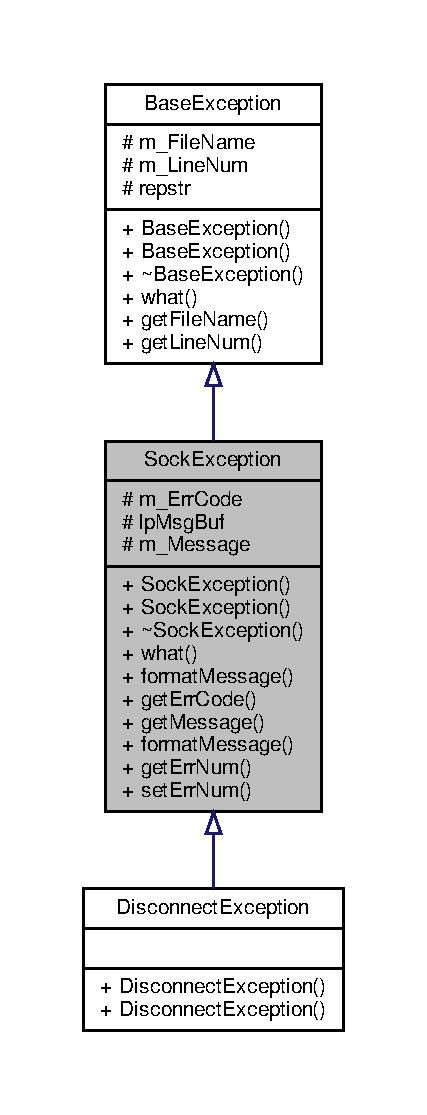
\includegraphics[width=205pt]{classSockException__inherit__graph}
\end{center}
\end{figure}
\subsection*{Public Member Functions}
\begin{DoxyCompactItemize}
\item 
\hyperlink{classSockException_a8ba3515f80c0b12b52dadbabf3778eef}{Sock\+Exception} (const char $\ast$File\+Name, int Line\+Num, int errcode)
\item 
\hyperlink{classSockException_ab0fa9e79b1f81f053821b399aebb8ccf}{Sock\+Exception} (const char $\ast$File\+Name, int Line\+Num, const char $\ast$Message)
\item 
virtual \hyperlink{classSockException_a29e9e5ac1de9ab65891c2310d764c60f}{$\sim$\+Sock\+Exception} ()  throw ()
\item 
virtual const char $\ast$ \hyperlink{classSockException_afb2986f2ddefe08ae1e735796cd05b1a}{what} ()
\item 
char $\ast$ \hyperlink{classSockException_a8c1eccb58e83020078f12f3050b7ac4f}{format\+Message} ()
\begin{DoxyCompactList}\small\item\em Format error message. \end{DoxyCompactList}\item 
int \hyperlink{classSockException_ab4dc853a2d0e855675327c54c0bd7301}{get\+Err\+Code} ()
\item 
char $\ast$ \hyperlink{classSockException_a198639b7111afd33d453e8bca22a7784}{get\+Message} ()
\end{DoxyCompactItemize}
\subsection*{Static Public Member Functions}
\begin{DoxyCompactItemize}
\item 
static bool \hyperlink{classSockException_ab830154d70e966c979585a1d285dd990}{format\+Message} (char($\ast$Msg\+Buf)\mbox{[}256\mbox{]})
\begin{DoxyCompactList}\small\item\em Format error message. \end{DoxyCompactList}\item 
static int \hyperlink{classSockException_a2539deadacaa23d71da34028d3f2ebc6}{get\+Err\+Num} ()
\item 
static void \hyperlink{classSockException_aa11513eff91eeed1cc5d098951700823}{set\+Err\+Num} (int Num=0)
\end{DoxyCompactItemize}
\subsection*{Protected Attributes}
\begin{DoxyCompactItemize}
\item 
int \hyperlink{classSockException_aa0b3cd8672ed45e8f61f0c94517d237c}{m\+\_\+\+Err\+Code}
\begin{DoxyCompactList}\small\item\em Error code. \end{DoxyCompactList}\item 
char \hyperlink{classSockException_a20f0f8c9f9c66905bba850c5ee508797}{lp\+Msg\+Buf} \mbox{[}256\mbox{]}
\begin{DoxyCompactList}\small\item\em Error message buffer. \end{DoxyCompactList}\item 
char \hyperlink{classSockException_ac9190a7ac09341189d5dfab54430c258}{m\+\_\+\+Message} \mbox{[}256\mbox{]}
\begin{DoxyCompactList}\small\item\em User\+Message buffer. \end{DoxyCompactList}\end{DoxyCompactItemize}


\subsection{Detailed Description}
Socket class library exception. 

\subsection{Constructor \& Destructor Documentation}
\mbox{\Hypertarget{classSockException_a8ba3515f80c0b12b52dadbabf3778eef}\label{classSockException_a8ba3515f80c0b12b52dadbabf3778eef}} 
\index{Sock\+Exception@{Sock\+Exception}!Sock\+Exception@{Sock\+Exception}}
\index{Sock\+Exception@{Sock\+Exception}!Sock\+Exception@{Sock\+Exception}}
\subsubsection{\texorpdfstring{Sock\+Exception()}{SockException()}\hspace{0.1cm}{\footnotesize\ttfamily [1/2]}}
{\footnotesize\ttfamily Sock\+Exception\+::\+Sock\+Exception (\begin{DoxyParamCaption}\item[{const char $\ast$}]{File\+Name,  }\item[{int}]{Line\+Num,  }\item[{int}]{errcode }\end{DoxyParamCaption})}

Constructor

Constructs exception object with filename and line number. 
\begin{DoxyParams}{Parameters}
{\em File\+Name} & \+: name of source file. \\
\hline
{\em Line\+Num} & \+: number of code line. \\
\hline
{\em errcode} & \+: error numeric code. \\
\hline
\end{DoxyParams}
\mbox{\Hypertarget{classSockException_ab0fa9e79b1f81f053821b399aebb8ccf}\label{classSockException_ab0fa9e79b1f81f053821b399aebb8ccf}} 
\index{Sock\+Exception@{Sock\+Exception}!Sock\+Exception@{Sock\+Exception}}
\index{Sock\+Exception@{Sock\+Exception}!Sock\+Exception@{Sock\+Exception}}
\subsubsection{\texorpdfstring{Sock\+Exception()}{SockException()}\hspace{0.1cm}{\footnotesize\ttfamily [2/2]}}
{\footnotesize\ttfamily Sock\+Exception\+::\+Sock\+Exception (\begin{DoxyParamCaption}\item[{const char $\ast$}]{File\+Name,  }\item[{int}]{Line\+Num,  }\item[{const char $\ast$}]{Message }\end{DoxyParamCaption})}

Constructor

Constructs exception object with filename, line number and text message 
\begin{DoxyParams}{Parameters}
{\em File\+Name} & \+: name of source file. \\
\hline
{\em Line\+Num} & \+: number of code line. \\
\hline
{\em Message} & \+: user message. \\
\hline
\end{DoxyParams}
\mbox{\Hypertarget{classSockException_a29e9e5ac1de9ab65891c2310d764c60f}\label{classSockException_a29e9e5ac1de9ab65891c2310d764c60f}} 
\index{Sock\+Exception@{Sock\+Exception}!````~Sock\+Exception@{$\sim$\+Sock\+Exception}}
\index{````~Sock\+Exception@{$\sim$\+Sock\+Exception}!Sock\+Exception@{Sock\+Exception}}
\subsubsection{\texorpdfstring{$\sim$\+Sock\+Exception()}{~SockException()}}
{\footnotesize\ttfamily virtual Sock\+Exception\+::$\sim$\+Sock\+Exception (\begin{DoxyParamCaption}{ }\end{DoxyParamCaption}) throw  ) \hspace{0.3cm}{\ttfamily [inline]}, {\ttfamily [virtual]}}

Destructor

Intentionally empty 

\subsection{Member Function Documentation}
\mbox{\Hypertarget{classSockException_a8c1eccb58e83020078f12f3050b7ac4f}\label{classSockException_a8c1eccb58e83020078f12f3050b7ac4f}} 
\index{Sock\+Exception@{Sock\+Exception}!format\+Message@{format\+Message}}
\index{format\+Message@{format\+Message}!Sock\+Exception@{Sock\+Exception}}
\subsubsection{\texorpdfstring{format\+Message()}{formatMessage()}\hspace{0.1cm}{\footnotesize\ttfamily [1/2]}}
{\footnotesize\ttfamily char $\ast$ Sock\+Exception\+::format\+Message (\begin{DoxyParamCaption}{ }\end{DoxyParamCaption})}



Format error message. 

\mbox{\Hypertarget{classSockException_ab830154d70e966c979585a1d285dd990}\label{classSockException_ab830154d70e966c979585a1d285dd990}} 
\index{Sock\+Exception@{Sock\+Exception}!format\+Message@{format\+Message}}
\index{format\+Message@{format\+Message}!Sock\+Exception@{Sock\+Exception}}
\subsubsection{\texorpdfstring{format\+Message()}{formatMessage()}\hspace{0.1cm}{\footnotesize\ttfamily [2/2]}}
{\footnotesize\ttfamily bool Sock\+Exception\+::format\+Message (\begin{DoxyParamCaption}\item[{char($\ast$)}]{Msg\+Buf\mbox{[}256\mbox{]} }\end{DoxyParamCaption})\hspace{0.3cm}{\ttfamily [static]}}



Format error message. 

\mbox{\Hypertarget{classSockException_ab4dc853a2d0e855675327c54c0bd7301}\label{classSockException_ab4dc853a2d0e855675327c54c0bd7301}} 
\index{Sock\+Exception@{Sock\+Exception}!get\+Err\+Code@{get\+Err\+Code}}
\index{get\+Err\+Code@{get\+Err\+Code}!Sock\+Exception@{Sock\+Exception}}
\subsubsection{\texorpdfstring{get\+Err\+Code()}{getErrCode()}}
{\footnotesize\ttfamily int Sock\+Exception\+::get\+Err\+Code (\begin{DoxyParamCaption}{ }\end{DoxyParamCaption})\hspace{0.3cm}{\ttfamily [inline]}}

Delivers error code \begin{DoxyReturn}{Returns}
error cod of the exception cause. 
\end{DoxyReturn}
\mbox{\Hypertarget{classSockException_a2539deadacaa23d71da34028d3f2ebc6}\label{classSockException_a2539deadacaa23d71da34028d3f2ebc6}} 
\index{Sock\+Exception@{Sock\+Exception}!get\+Err\+Num@{get\+Err\+Num}}
\index{get\+Err\+Num@{get\+Err\+Num}!Sock\+Exception@{Sock\+Exception}}
\subsubsection{\texorpdfstring{get\+Err\+Num()}{getErrNum()}}
{\footnotesize\ttfamily static int Sock\+Exception\+::get\+Err\+Num (\begin{DoxyParamCaption}{ }\end{DoxyParamCaption})\hspace{0.3cm}{\ttfamily [inline]}, {\ttfamily [static]}}

Delivers errno \begin{DoxyReturn}{Returns}
errno 
\end{DoxyReturn}
\mbox{\Hypertarget{classSockException_a198639b7111afd33d453e8bca22a7784}\label{classSockException_a198639b7111afd33d453e8bca22a7784}} 
\index{Sock\+Exception@{Sock\+Exception}!get\+Message@{get\+Message}}
\index{get\+Message@{get\+Message}!Sock\+Exception@{Sock\+Exception}}
\subsubsection{\texorpdfstring{get\+Message()}{getMessage()}}
{\footnotesize\ttfamily char$\ast$ Sock\+Exception\+::get\+Message (\begin{DoxyParamCaption}{ }\end{DoxyParamCaption})\hspace{0.3cm}{\ttfamily [inline]}}

Delivers error message. \begin{DoxyReturn}{Returns}
message buffer. 
\end{DoxyReturn}
\mbox{\Hypertarget{classSockException_aa11513eff91eeed1cc5d098951700823}\label{classSockException_aa11513eff91eeed1cc5d098951700823}} 
\index{Sock\+Exception@{Sock\+Exception}!set\+Err\+Num@{set\+Err\+Num}}
\index{set\+Err\+Num@{set\+Err\+Num}!Sock\+Exception@{Sock\+Exception}}
\subsubsection{\texorpdfstring{set\+Err\+Num()}{setErrNum()}}
{\footnotesize\ttfamily static void Sock\+Exception\+::set\+Err\+Num (\begin{DoxyParamCaption}\item[{int}]{Num = {\ttfamily 0} }\end{DoxyParamCaption})\hspace{0.3cm}{\ttfamily [inline]}, {\ttfamily [static]}}

Sets error number. 
\begin{DoxyParams}{Parameters}
{\em Num} & \+: error number. \\
\hline
\end{DoxyParams}
\mbox{\Hypertarget{classSockException_afb2986f2ddefe08ae1e735796cd05b1a}\label{classSockException_afb2986f2ddefe08ae1e735796cd05b1a}} 
\index{Sock\+Exception@{Sock\+Exception}!what@{what}}
\index{what@{what}!Sock\+Exception@{Sock\+Exception}}
\subsubsection{\texorpdfstring{what()}{what()}}
{\footnotesize\ttfamily const char $\ast$ Sock\+Exception\+::what (\begin{DoxyParamCaption}{ }\end{DoxyParamCaption})\hspace{0.3cm}{\ttfamily [virtual]}}

Reports exception\textquotesingle{}s properties. \begin{DoxyReturn}{Returns}
String buffer with report text. 
\end{DoxyReturn}


Reimplemented from \hyperlink{group__EXCEPT__GROUP_gaf092dd6587491cd7a8cdd987597b1018}{Base\+Exception}.



\subsection{Member Data Documentation}
\mbox{\Hypertarget{classSockException_a20f0f8c9f9c66905bba850c5ee508797}\label{classSockException_a20f0f8c9f9c66905bba850c5ee508797}} 
\index{Sock\+Exception@{Sock\+Exception}!lp\+Msg\+Buf@{lp\+Msg\+Buf}}
\index{lp\+Msg\+Buf@{lp\+Msg\+Buf}!Sock\+Exception@{Sock\+Exception}}
\subsubsection{\texorpdfstring{lp\+Msg\+Buf}{lpMsgBuf}}
{\footnotesize\ttfamily char Sock\+Exception\+::lp\+Msg\+Buf\mbox{[}256\mbox{]}\hspace{0.3cm}{\ttfamily [protected]}}



Error message buffer. 

\mbox{\Hypertarget{classSockException_aa0b3cd8672ed45e8f61f0c94517d237c}\label{classSockException_aa0b3cd8672ed45e8f61f0c94517d237c}} 
\index{Sock\+Exception@{Sock\+Exception}!m\+\_\+\+Err\+Code@{m\+\_\+\+Err\+Code}}
\index{m\+\_\+\+Err\+Code@{m\+\_\+\+Err\+Code}!Sock\+Exception@{Sock\+Exception}}
\subsubsection{\texorpdfstring{m\+\_\+\+Err\+Code}{m\_ErrCode}}
{\footnotesize\ttfamily int Sock\+Exception\+::m\+\_\+\+Err\+Code\hspace{0.3cm}{\ttfamily [protected]}}



Error code. 

\mbox{\Hypertarget{classSockException_ac9190a7ac09341189d5dfab54430c258}\label{classSockException_ac9190a7ac09341189d5dfab54430c258}} 
\index{Sock\+Exception@{Sock\+Exception}!m\+\_\+\+Message@{m\+\_\+\+Message}}
\index{m\+\_\+\+Message@{m\+\_\+\+Message}!Sock\+Exception@{Sock\+Exception}}
\subsubsection{\texorpdfstring{m\+\_\+\+Message}{m\_Message}}
{\footnotesize\ttfamily char Sock\+Exception\+::m\+\_\+\+Message\mbox{[}256\mbox{]}\hspace{0.3cm}{\ttfamily [protected]}}



User\+Message buffer. 



The documentation for this class was generated from the following files\+:\begin{DoxyCompactItemize}
\item 
\hyperlink{SockException_8h}{Sock\+Exception.\+h}\item 
\hyperlink{SockException_8cpp}{Sock\+Exception.\+cpp}\end{DoxyCompactItemize}

\hypertarget{classStreamBoundV4}{}\section{Stream\+Bound\+V4 Class Reference}
\label{classStreamBoundV4}\index{Stream\+Bound\+V4@{Stream\+Bound\+V4}}


T\+CP socket bound to specified port and address.  




{\ttfamily \#include $<$Stream\+Bound\+V4.\+h$>$}



Inheritance diagram for Stream\+Bound\+V4\+:\nopagebreak
\begin{figure}[H]
\begin{center}
\leavevmode
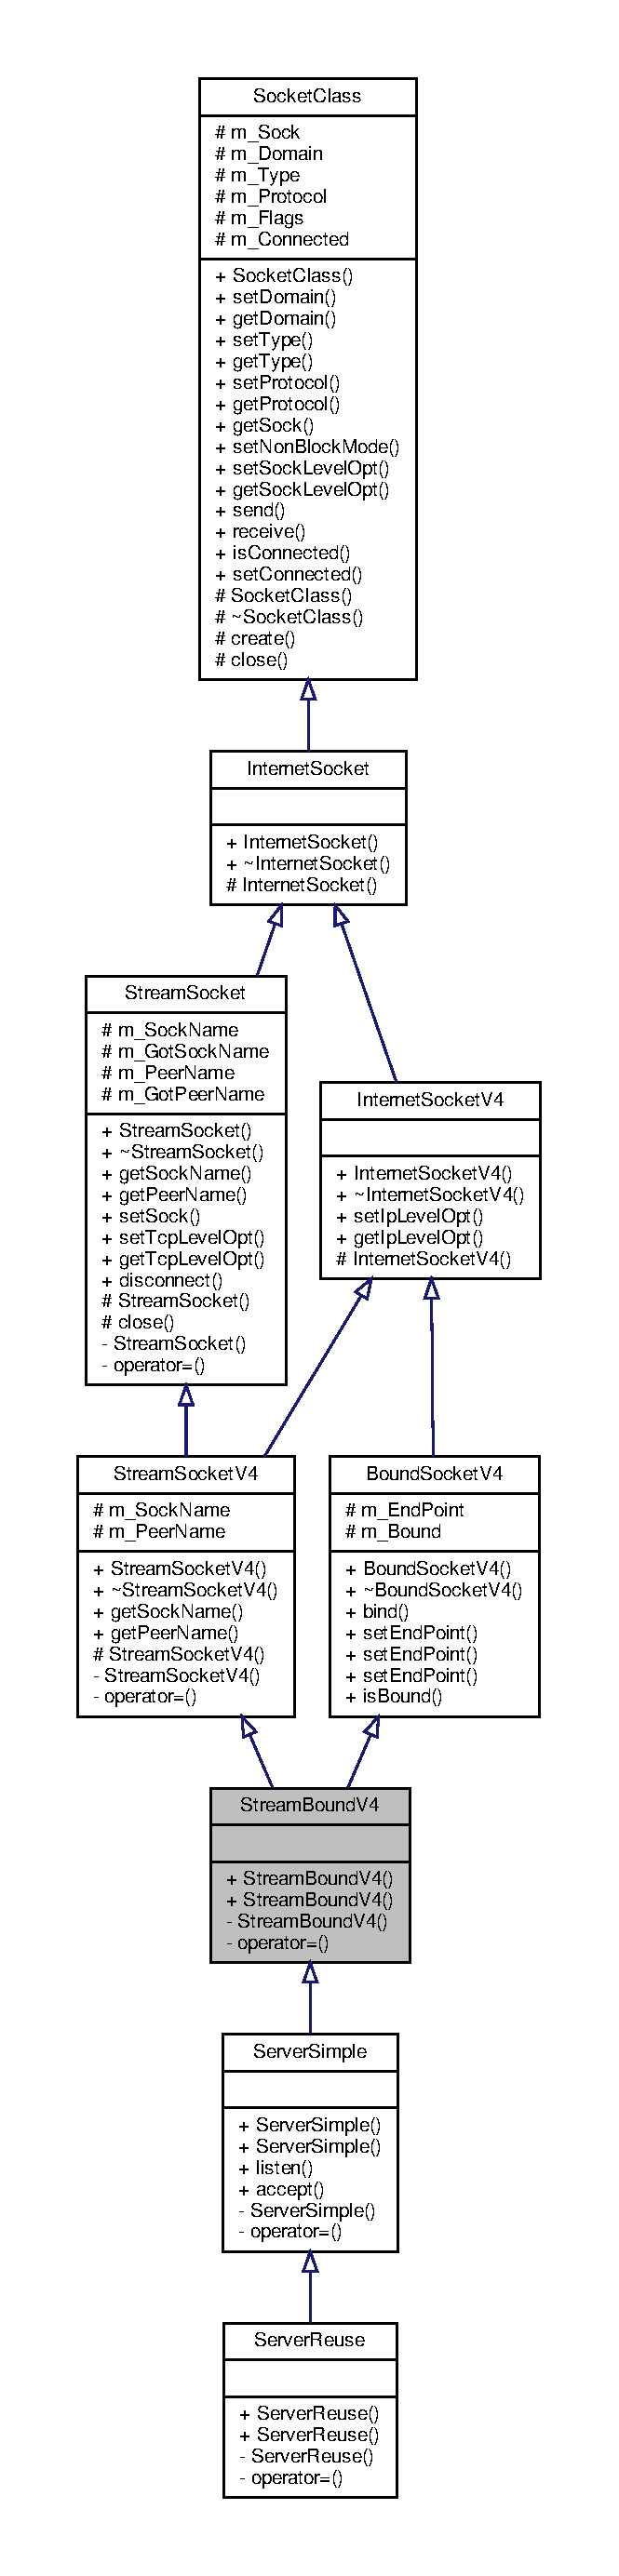
\includegraphics[height=550pt]{classStreamBoundV4__inherit__graph}
\end{center}
\end{figure}
\subsection*{Public Member Functions}
\begin{DoxyCompactItemize}
\item 
\hyperlink{classStreamBoundV4_ae29ec7a9e59a9e3aef01c4251113cbca}{Stream\+Bound\+V4} (short Port, in\+\_\+addr\+\_\+t Address=I\+N\+A\+D\+D\+R\+\_\+\+A\+NY, bool Late\+Bind=false)
\item 
\hyperlink{classStreamBoundV4_ab070a58759e73f5407b4766d1629c708}{Stream\+Bound\+V4} (short Port, const char $\ast$Address, bool Late\+Bind=false)
\end{DoxyCompactItemize}
\subsection*{Private Member Functions}
\begin{DoxyCompactItemize}
\item 
\hyperlink{classStreamBoundV4_a8a78f05c41413598bfc662417e8dbeb5}{Stream\+Bound\+V4} (\hyperlink{classStreamBoundV4}{Stream\+Bound\+V4} \&s)
\item 
\hyperlink{classStreamBoundV4}{Stream\+Bound\+V4} \& \hyperlink{classStreamBoundV4_a762eb400e5cfc54f2f2f5b1df48a616e}{operator=} (\hyperlink{classStreamBoundV4}{Stream\+Bound\+V4} \&s)
\end{DoxyCompactItemize}
\subsection*{Additional Inherited Members}


\subsection{Detailed Description}
T\+CP socket bound to specified port and address. 

\subsection{Constructor \& Destructor Documentation}
\mbox{\Hypertarget{classStreamBoundV4_ae29ec7a9e59a9e3aef01c4251113cbca}\label{classStreamBoundV4_ae29ec7a9e59a9e3aef01c4251113cbca}} 
\index{Stream\+Bound\+V4@{Stream\+Bound\+V4}!Stream\+Bound\+V4@{Stream\+Bound\+V4}}
\index{Stream\+Bound\+V4@{Stream\+Bound\+V4}!Stream\+Bound\+V4@{Stream\+Bound\+V4}}
\subsubsection{\texorpdfstring{Stream\+Bound\+V4()}{StreamBoundV4()}\hspace{0.1cm}{\footnotesize\ttfamily [1/3]}}
{\footnotesize\ttfamily Stream\+Bound\+V4\+::\+Stream\+Bound\+V4 (\begin{DoxyParamCaption}\item[{short}]{Port,  }\item[{in\+\_\+addr\+\_\+t}]{Address = {\ttfamily INADDR\+\_\+ANY},  }\item[{bool}]{Late\+Bind = {\ttfamily false} }\end{DoxyParamCaption})}

Constructor. 
\begin{DoxyParams}{Parameters}
{\em Port} & \+: port number for bind in network byte order. \\
\hline
{\em Address} & \+: I\+Pv4 address for bind in network byte order. \\
\hline
{\em Late\+Bind} & \+: do bind now or later according to bind method call. \\
\hline
\end{DoxyParams}

\begin{DoxyExceptions}{Exceptions}
{\em Sock\+Exception.} & \\
\hline
\end{DoxyExceptions}
\mbox{\Hypertarget{classStreamBoundV4_ab070a58759e73f5407b4766d1629c708}\label{classStreamBoundV4_ab070a58759e73f5407b4766d1629c708}} 
\index{Stream\+Bound\+V4@{Stream\+Bound\+V4}!Stream\+Bound\+V4@{Stream\+Bound\+V4}}
\index{Stream\+Bound\+V4@{Stream\+Bound\+V4}!Stream\+Bound\+V4@{Stream\+Bound\+V4}}
\subsubsection{\texorpdfstring{Stream\+Bound\+V4()}{StreamBoundV4()}\hspace{0.1cm}{\footnotesize\ttfamily [2/3]}}
{\footnotesize\ttfamily Stream\+Bound\+V4\+::\+Stream\+Bound\+V4 (\begin{DoxyParamCaption}\item[{short}]{Port,  }\item[{const char $\ast$}]{Address,  }\item[{bool}]{Late\+Bind = {\ttfamily false} }\end{DoxyParamCaption})}

Constructor. 
\begin{DoxyParams}{Parameters}
{\em Port} & \+: port number for bind in network byte order. \\
\hline
{\em Address} & \+: I\+Pv4 address for bind in decimal dot notation. \\
\hline
{\em Late\+Bind} & \+: do bind now or later according to bind method call. \\
\hline
\end{DoxyParams}

\begin{DoxyExceptions}{Exceptions}
{\em Sock\+Exception.} & \\
\hline
\end{DoxyExceptions}
\mbox{\Hypertarget{classStreamBoundV4_a8a78f05c41413598bfc662417e8dbeb5}\label{classStreamBoundV4_a8a78f05c41413598bfc662417e8dbeb5}} 
\index{Stream\+Bound\+V4@{Stream\+Bound\+V4}!Stream\+Bound\+V4@{Stream\+Bound\+V4}}
\index{Stream\+Bound\+V4@{Stream\+Bound\+V4}!Stream\+Bound\+V4@{Stream\+Bound\+V4}}
\subsubsection{\texorpdfstring{Stream\+Bound\+V4()}{StreamBoundV4()}\hspace{0.1cm}{\footnotesize\ttfamily [3/3]}}
{\footnotesize\ttfamily Stream\+Bound\+V4\+::\+Stream\+Bound\+V4 (\begin{DoxyParamCaption}\item[{\hyperlink{classStreamBoundV4}{Stream\+Bound\+V4} \&}]{s }\end{DoxyParamCaption})\hspace{0.3cm}{\ttfamily [private]}}

Copy constructor. Makes the class uncopyable. 

\subsection{Member Function Documentation}
\mbox{\Hypertarget{classStreamBoundV4_a762eb400e5cfc54f2f2f5b1df48a616e}\label{classStreamBoundV4_a762eb400e5cfc54f2f2f5b1df48a616e}} 
\index{Stream\+Bound\+V4@{Stream\+Bound\+V4}!operator=@{operator=}}
\index{operator=@{operator=}!Stream\+Bound\+V4@{Stream\+Bound\+V4}}
\subsubsection{\texorpdfstring{operator=()}{operator=()}}
{\footnotesize\ttfamily \hyperlink{classStreamBoundV4}{Stream\+Bound\+V4}\& Stream\+Bound\+V4\+::operator= (\begin{DoxyParamCaption}\item[{\hyperlink{classStreamBoundV4}{Stream\+Bound\+V4} \&}]{s }\end{DoxyParamCaption})\hspace{0.3cm}{\ttfamily [private]}}

Operator assign. Makes the class uncopyable. 

The documentation for this class was generated from the following files\+:\begin{DoxyCompactItemize}
\item 
\hyperlink{StreamBoundV4_8h}{Stream\+Bound\+V4.\+h}\item 
\hyperlink{StreamBoundV4_8cpp}{Stream\+Bound\+V4.\+cpp}\end{DoxyCompactItemize}

\hypertarget{classStreamBoundV6}{}\section{Stream\+Bound\+V6 Class Reference}
\label{classStreamBoundV6}\index{Stream\+Bound\+V6@{Stream\+Bound\+V6}}


T\+CP socket bound to specified port and address.  




{\ttfamily \#include $<$Stream\+Bound\+V6.\+h$>$}



Inheritance diagram for Stream\+Bound\+V6\+:\nopagebreak
\begin{figure}[H]
\begin{center}
\leavevmode
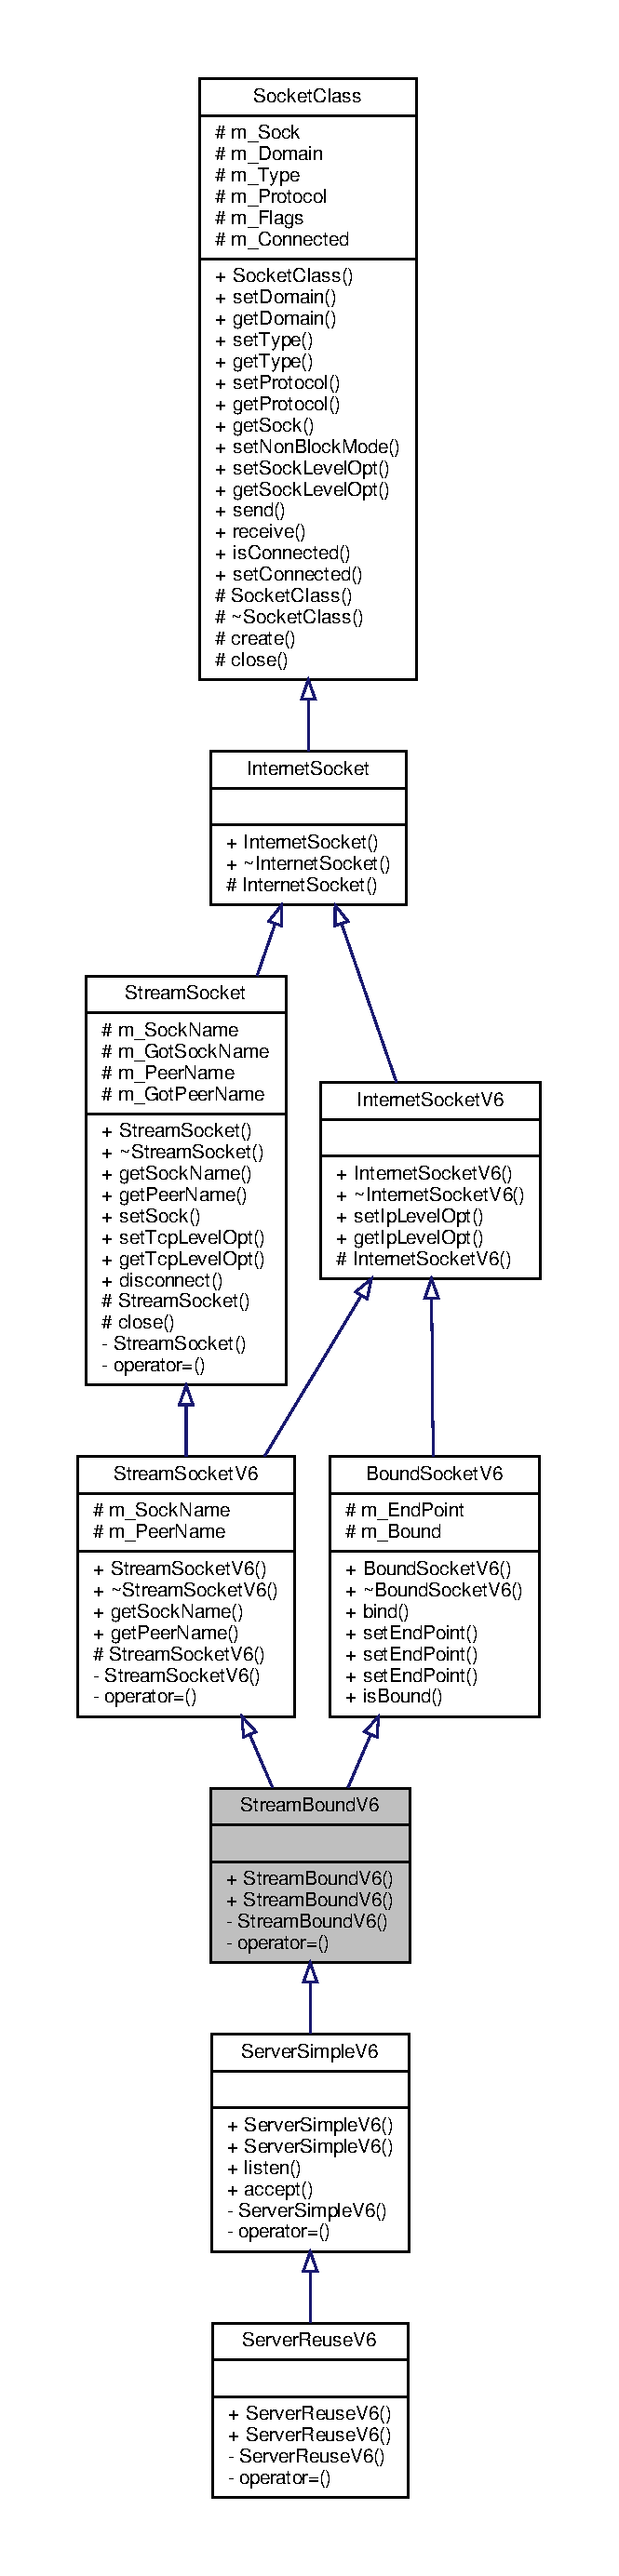
\includegraphics[height=550pt]{classStreamBoundV6__inherit__graph}
\end{center}
\end{figure}
\subsection*{Public Member Functions}
\begin{DoxyCompactItemize}
\item 
\hyperlink{classStreamBoundV6_a81d2ecafcbb417fe6e319daa8335be18}{Stream\+Bound\+V6} (short Port, in6\+\_\+addr Address=in6addr\+\_\+any, bool Late\+Bind=false)
\item 
\hyperlink{classStreamBoundV6_a2408b1863d8043ea8fc5a2f460e98fb5}{Stream\+Bound\+V6} (short Port, const char $\ast$Address, bool Late\+Bind=false)
\end{DoxyCompactItemize}
\subsection*{Private Member Functions}
\begin{DoxyCompactItemize}
\item 
\hyperlink{classStreamBoundV6_a90747cdecae8ad1ef744cad16e7d9ae1}{Stream\+Bound\+V6} (\hyperlink{classStreamBoundV6}{Stream\+Bound\+V6} \&s)
\item 
\hyperlink{classStreamBoundV6}{Stream\+Bound\+V6} \& \hyperlink{classStreamBoundV6_ad5f53565b680b46896fe8ab713d658f9}{operator=} (\hyperlink{classStreamBoundV6}{Stream\+Bound\+V6} \&s)
\end{DoxyCompactItemize}
\subsection*{Additional Inherited Members}


\subsection{Detailed Description}
T\+CP socket bound to specified port and address. 

\subsection{Constructor \& Destructor Documentation}
\mbox{\Hypertarget{classStreamBoundV6_a81d2ecafcbb417fe6e319daa8335be18}\label{classStreamBoundV6_a81d2ecafcbb417fe6e319daa8335be18}} 
\index{Stream\+Bound\+V6@{Stream\+Bound\+V6}!Stream\+Bound\+V6@{Stream\+Bound\+V6}}
\index{Stream\+Bound\+V6@{Stream\+Bound\+V6}!Stream\+Bound\+V6@{Stream\+Bound\+V6}}
\subsubsection{\texorpdfstring{Stream\+Bound\+V6()}{StreamBoundV6()}\hspace{0.1cm}{\footnotesize\ttfamily [1/3]}}
{\footnotesize\ttfamily Stream\+Bound\+V6\+::\+Stream\+Bound\+V6 (\begin{DoxyParamCaption}\item[{short}]{Port,  }\item[{in6\+\_\+addr}]{Address = {\ttfamily in6addr\+\_\+any},  }\item[{bool}]{Late\+Bind = {\ttfamily false} }\end{DoxyParamCaption})}

Constructor. 
\begin{DoxyParams}{Parameters}
{\em Port} & \+: port number for bind in network byte order. \\
\hline
{\em Address} & \+: I\+Pv6 address for bind. \\
\hline
{\em Late\+Bind} & \+: do bind now or later according to bind method call. \\
\hline
\end{DoxyParams}

\begin{DoxyExceptions}{Exceptions}
{\em Sock\+Exception.} & \\
\hline
\end{DoxyExceptions}
\mbox{\Hypertarget{classStreamBoundV6_a2408b1863d8043ea8fc5a2f460e98fb5}\label{classStreamBoundV6_a2408b1863d8043ea8fc5a2f460e98fb5}} 
\index{Stream\+Bound\+V6@{Stream\+Bound\+V6}!Stream\+Bound\+V6@{Stream\+Bound\+V6}}
\index{Stream\+Bound\+V6@{Stream\+Bound\+V6}!Stream\+Bound\+V6@{Stream\+Bound\+V6}}
\subsubsection{\texorpdfstring{Stream\+Bound\+V6()}{StreamBoundV6()}\hspace{0.1cm}{\footnotesize\ttfamily [2/3]}}
{\footnotesize\ttfamily Stream\+Bound\+V6\+::\+Stream\+Bound\+V6 (\begin{DoxyParamCaption}\item[{short}]{Port,  }\item[{const char $\ast$}]{Address,  }\item[{bool}]{Late\+Bind = {\ttfamily false} }\end{DoxyParamCaption})}

Constructor. 
\begin{DoxyParams}{Parameters}
{\em Port} & \+: port number for bind in network byte order. \\
\hline
{\em Address} & \+: I\+Pv6 address for bind in textual notation. \\
\hline
{\em Late\+Bind} & \+: do bind now or later according to bind method call. \\
\hline
\end{DoxyParams}

\begin{DoxyExceptions}{Exceptions}
{\em Sock\+Exception.} & \\
\hline
\end{DoxyExceptions}
\mbox{\Hypertarget{classStreamBoundV6_a90747cdecae8ad1ef744cad16e7d9ae1}\label{classStreamBoundV6_a90747cdecae8ad1ef744cad16e7d9ae1}} 
\index{Stream\+Bound\+V6@{Stream\+Bound\+V6}!Stream\+Bound\+V6@{Stream\+Bound\+V6}}
\index{Stream\+Bound\+V6@{Stream\+Bound\+V6}!Stream\+Bound\+V6@{Stream\+Bound\+V6}}
\subsubsection{\texorpdfstring{Stream\+Bound\+V6()}{StreamBoundV6()}\hspace{0.1cm}{\footnotesize\ttfamily [3/3]}}
{\footnotesize\ttfamily Stream\+Bound\+V6\+::\+Stream\+Bound\+V6 (\begin{DoxyParamCaption}\item[{\hyperlink{classStreamBoundV6}{Stream\+Bound\+V6} \&}]{s }\end{DoxyParamCaption})\hspace{0.3cm}{\ttfamily [private]}}

Copy constructor. Makes the class uncopyable. 

\subsection{Member Function Documentation}
\mbox{\Hypertarget{classStreamBoundV6_ad5f53565b680b46896fe8ab713d658f9}\label{classStreamBoundV6_ad5f53565b680b46896fe8ab713d658f9}} 
\index{Stream\+Bound\+V6@{Stream\+Bound\+V6}!operator=@{operator=}}
\index{operator=@{operator=}!Stream\+Bound\+V6@{Stream\+Bound\+V6}}
\subsubsection{\texorpdfstring{operator=()}{operator=()}}
{\footnotesize\ttfamily \hyperlink{classStreamBoundV6}{Stream\+Bound\+V6}\& Stream\+Bound\+V6\+::operator= (\begin{DoxyParamCaption}\item[{\hyperlink{classStreamBoundV6}{Stream\+Bound\+V6} \&}]{s }\end{DoxyParamCaption})\hspace{0.3cm}{\ttfamily [private]}}

Operator assign. Makes the class uncopyable. 

The documentation for this class was generated from the following files\+:\begin{DoxyCompactItemize}
\item 
\hyperlink{StreamBoundV6_8h}{Stream\+Bound\+V6.\+h}\item 
\hyperlink{StreamBoundV6_8cpp}{Stream\+Bound\+V6.\+cpp}\end{DoxyCompactItemize}

\hypertarget{classStreamSocket}{}\section{Stream\+Socket Class Reference}
\label{classStreamSocket}\index{Stream\+Socket@{Stream\+Socket}}


{\ttfamily \#include $<$Stream\+Socket.\+h$>$}



Inheritance diagram for Stream\+Socket\+:\nopagebreak
\begin{figure}[H]
\begin{center}
\leavevmode
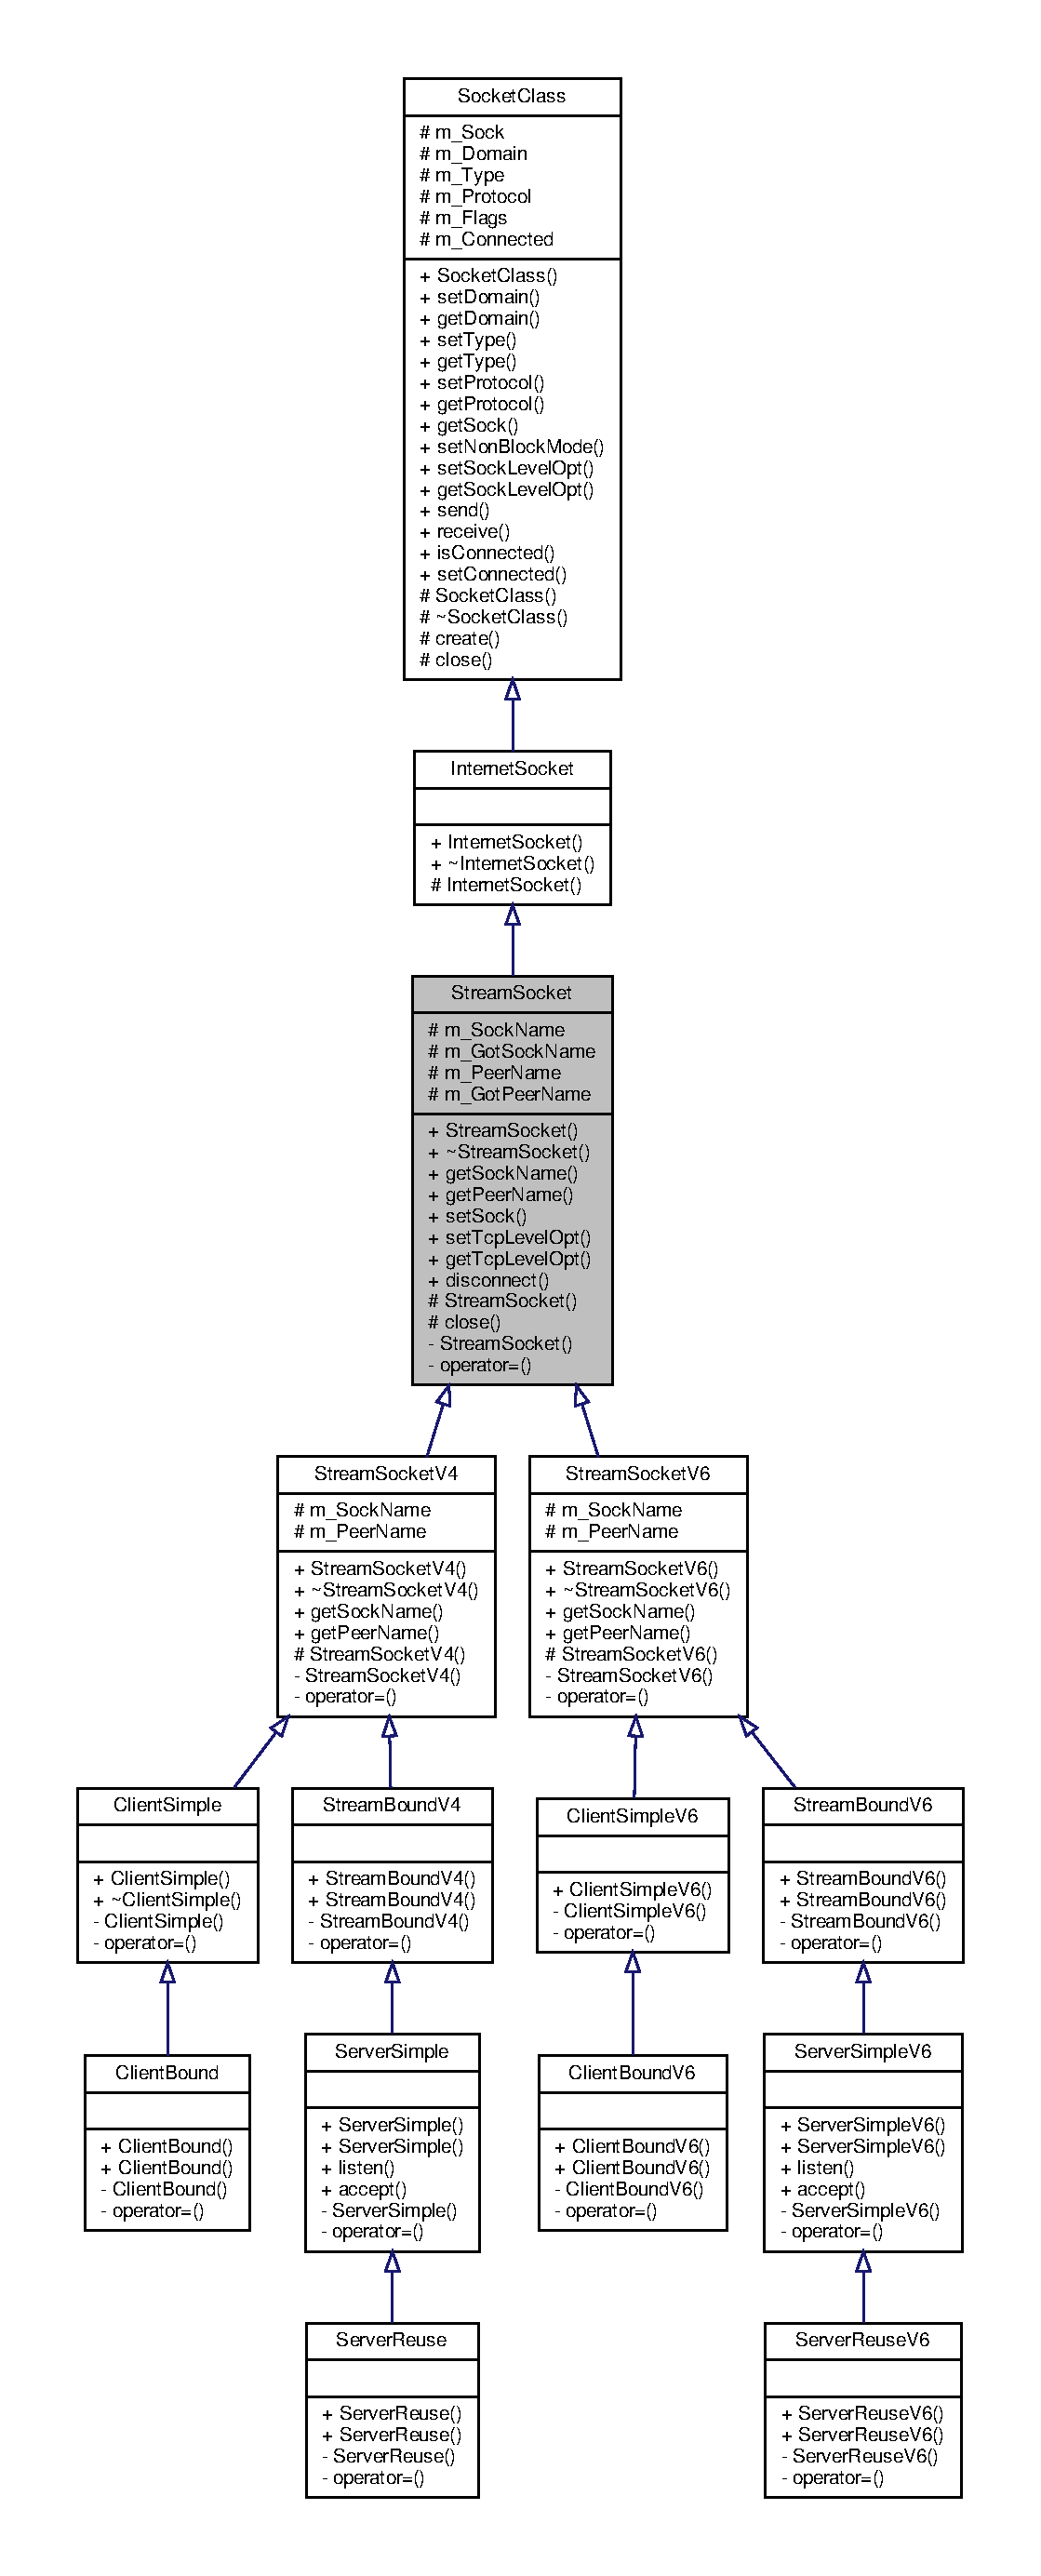
\includegraphics[height=550pt]{classStreamSocket__inherit__graph}
\end{center}
\end{figure}
\subsection*{Public Member Functions}
\begin{DoxyCompactItemize}
\item 
\hyperlink{classStreamSocket_a5b84a10f7bece6175c0d885c3568aa4f}{Stream\+Socket} (\hyperlink{sockclasslib_8h_a8dc8083897335125630f1af5dafd5831}{S\+O\+C\+K\+ET} sock)
\item 
virtual \hyperlink{classStreamSocket_ad19381c15cf7390ea3751d930b16c45e}{$\sim$\+Stream\+Socket} ()
\begin{DoxyCompactList}\small\item\em Destructor. \end{DoxyCompactList}\item 
sockaddr\+\_\+in \& \hyperlink{classStreamSocket_ab634d93813e97a292ae8b29fd9d39bcd}{get\+Sock\+Name} ()
\item 
sockaddr\+\_\+in \& \hyperlink{classStreamSocket_ab9065328673e08e0fb5df8eefda3604d}{get\+Peer\+Name} ()
\item 
void \hyperlink{classStreamSocket_a644c75a180ea636ab4373a903062a4ad}{set\+Sock} (int i)
\item 
void \hyperlink{classStreamSocket_a776cd788e6f324f41febfb71b03e8cc7}{set\+Tcp\+Level\+Opt} (int Opt, const char $\ast$Value, int Opt\+Len)
\item 
void \hyperlink{classStreamSocket_a5ad690e49784bbfa352232724529ae4c}{get\+Tcp\+Level\+Opt} (int Opt, char $\ast$Value, int $\ast$Opt\+Len)
\item 
void \hyperlink{classStreamSocket_a01cd43dea5b792a72d741288f840b08b}{disconnect} (long Timeout=0)
\end{DoxyCompactItemize}
\subsection*{Protected Member Functions}
\begin{DoxyCompactItemize}
\item 
\hyperlink{classStreamSocket_a005683fb7badf43a1d0a30b9ad09649e}{Stream\+Socket} ()
\begin{DoxyCompactList}\small\item\em Constructor. \end{DoxyCompactList}\item 
virtual void \hyperlink{classStreamSocket_a9dc930d6a0f7d6a8b96631348297bce2}{close} ()
\begin{DoxyCompactList}\small\item\em Close the socket. \end{DoxyCompactList}\end{DoxyCompactItemize}
\subsection*{Protected Attributes}
\begin{DoxyCompactItemize}
\item 
sockaddr\+\_\+in \hyperlink{classStreamSocket_a3d9ba37dc44b6ebcbb836f1aeb90ec74}{m\+\_\+\+Sock\+Name}
\begin{DoxyCompactList}\small\item\em Bound endpoint properties. \end{DoxyCompactList}\item 
bool \hyperlink{classStreamSocket_a4f019df008ee69c34332f0e08c68d746}{m\+\_\+\+Got\+Sock\+Name}
\begin{DoxyCompactList}\small\item\em Bound endpoint properties are filled. \end{DoxyCompactList}\item 
sockaddr\+\_\+in \hyperlink{classStreamSocket_a4ab3bf06cf2d7866f36091258d3bd20a}{m\+\_\+\+Peer\+Name}
\begin{DoxyCompactList}\small\item\em Destination endpoint properties. \end{DoxyCompactList}\item 
bool \hyperlink{classStreamSocket_a14305f0d399b0b4bab1b8e1b8fa99844}{m\+\_\+\+Got\+Peer\+Name}
\begin{DoxyCompactList}\small\item\em Destination endpoint properties are filled. \end{DoxyCompactList}\end{DoxyCompactItemize}
\subsection*{Private Member Functions}
\begin{DoxyCompactItemize}
\item 
\hyperlink{classStreamSocket_a11756527c7644ee85bc2debfd8aef576}{Stream\+Socket} (\hyperlink{classStreamSocket}{Stream\+Socket} \&s)
\item 
\hyperlink{classStreamSocket}{Stream\+Socket} \& \hyperlink{classStreamSocket_a4b78db9579afcfe387af3335c632ba49}{operator=} (\hyperlink{classStreamSocket}{Stream\+Socket} \&s)
\end{DoxyCompactItemize}
\subsection*{Friends}
\begin{DoxyCompactItemize}
\item 
class \hyperlink{classStreamSocket_afa2b19845876e6ba2e47d2393147ff4b}{Server\+Simple}
\item 
class \hyperlink{classStreamSocket_ad693c1bdff496f6dc8b4268108014bf2}{Server\+Simple\+V6}
\end{DoxyCompactItemize}
\subsection*{Additional Inherited Members}


\subsection{Detailed Description}
Stream socket class. The base class for all stream-\/oriented sockets. 

\subsection{Constructor \& Destructor Documentation}
\mbox{\Hypertarget{classStreamSocket_a5b84a10f7bece6175c0d885c3568aa4f}\label{classStreamSocket_a5b84a10f7bece6175c0d885c3568aa4f}} 
\index{Stream\+Socket@{Stream\+Socket}!Stream\+Socket@{Stream\+Socket}}
\index{Stream\+Socket@{Stream\+Socket}!Stream\+Socket@{Stream\+Socket}}
\subsubsection{\texorpdfstring{Stream\+Socket()}{StreamSocket()}\hspace{0.1cm}{\footnotesize\ttfamily [1/3]}}
{\footnotesize\ttfamily Stream\+Socket\+::\+Stream\+Socket (\begin{DoxyParamCaption}\item[{\hyperlink{sockclasslib_8h_a8dc8083897335125630f1af5dafd5831}{S\+O\+C\+K\+ET}}]{sock }\end{DoxyParamCaption})}

Constructor. 
\begin{DoxyParams}{Parameters}
{\em sock} & \+: socket file descriptor/handle. \\
\hline
\end{DoxyParams}
\mbox{\Hypertarget{classStreamSocket_ad19381c15cf7390ea3751d930b16c45e}\label{classStreamSocket_ad19381c15cf7390ea3751d930b16c45e}} 
\index{Stream\+Socket@{Stream\+Socket}!````~Stream\+Socket@{$\sim$\+Stream\+Socket}}
\index{````~Stream\+Socket@{$\sim$\+Stream\+Socket}!Stream\+Socket@{Stream\+Socket}}
\subsubsection{\texorpdfstring{$\sim$\+Stream\+Socket()}{~StreamSocket()}}
{\footnotesize\ttfamily virtual Stream\+Socket\+::$\sim$\+Stream\+Socket (\begin{DoxyParamCaption}{ }\end{DoxyParamCaption})\hspace{0.3cm}{\ttfamily [inline]}, {\ttfamily [virtual]}}



Destructor. 

\mbox{\Hypertarget{classStreamSocket_a005683fb7badf43a1d0a30b9ad09649e}\label{classStreamSocket_a005683fb7badf43a1d0a30b9ad09649e}} 
\index{Stream\+Socket@{Stream\+Socket}!Stream\+Socket@{Stream\+Socket}}
\index{Stream\+Socket@{Stream\+Socket}!Stream\+Socket@{Stream\+Socket}}
\subsubsection{\texorpdfstring{Stream\+Socket()}{StreamSocket()}\hspace{0.1cm}{\footnotesize\ttfamily [2/3]}}
{\footnotesize\ttfamily Stream\+Socket\+::\+Stream\+Socket (\begin{DoxyParamCaption}{ }\end{DoxyParamCaption})\hspace{0.3cm}{\ttfamily [protected]}}



Constructor. 

\mbox{\Hypertarget{classStreamSocket_a11756527c7644ee85bc2debfd8aef576}\label{classStreamSocket_a11756527c7644ee85bc2debfd8aef576}} 
\index{Stream\+Socket@{Stream\+Socket}!Stream\+Socket@{Stream\+Socket}}
\index{Stream\+Socket@{Stream\+Socket}!Stream\+Socket@{Stream\+Socket}}
\subsubsection{\texorpdfstring{Stream\+Socket()}{StreamSocket()}\hspace{0.1cm}{\footnotesize\ttfamily [3/3]}}
{\footnotesize\ttfamily Stream\+Socket\+::\+Stream\+Socket (\begin{DoxyParamCaption}\item[{\hyperlink{classStreamSocket}{Stream\+Socket} \&}]{s }\end{DoxyParamCaption})\hspace{0.3cm}{\ttfamily [private]}}

Constructor. Copy constructor. Makes the class uncopyable. 

\subsection{Member Function Documentation}
\mbox{\Hypertarget{classStreamSocket_a9dc930d6a0f7d6a8b96631348297bce2}\label{classStreamSocket_a9dc930d6a0f7d6a8b96631348297bce2}} 
\index{Stream\+Socket@{Stream\+Socket}!close@{close}}
\index{close@{close}!Stream\+Socket@{Stream\+Socket}}
\subsubsection{\texorpdfstring{close()}{close()}}
{\footnotesize\ttfamily virtual void Stream\+Socket\+::close (\begin{DoxyParamCaption}{ }\end{DoxyParamCaption})\hspace{0.3cm}{\ttfamily [inline]}, {\ttfamily [protected]}, {\ttfamily [virtual]}}



Close the socket. 



Implements \hyperlink{classSocketClass_a92c8c1b22b98f0231932cbd84cdc4cfe}{Socket\+Class}.

\mbox{\Hypertarget{classStreamSocket_a01cd43dea5b792a72d741288f840b08b}\label{classStreamSocket_a01cd43dea5b792a72d741288f840b08b}} 
\index{Stream\+Socket@{Stream\+Socket}!disconnect@{disconnect}}
\index{disconnect@{disconnect}!Stream\+Socket@{Stream\+Socket}}
\subsubsection{\texorpdfstring{disconnect()}{disconnect()}}
{\footnotesize\ttfamily void Stream\+Socket\+::disconnect (\begin{DoxyParamCaption}\item[{long}]{Timeout = {\ttfamily 0} }\end{DoxyParamCaption})}

Disconnect endpoint. 
\begin{DoxyParams}{Parameters}
{\em Timeout} & \+: Time to wait for orderly close the socket in milliseconds. \\
\hline
\end{DoxyParams}
\mbox{\Hypertarget{classStreamSocket_ab9065328673e08e0fb5df8eefda3604d}\label{classStreamSocket_ab9065328673e08e0fb5df8eefda3604d}} 
\index{Stream\+Socket@{Stream\+Socket}!get\+Peer\+Name@{get\+Peer\+Name}}
\index{get\+Peer\+Name@{get\+Peer\+Name}!Stream\+Socket@{Stream\+Socket}}
\subsubsection{\texorpdfstring{get\+Peer\+Name()}{getPeerName()}}
{\footnotesize\ttfamily sockaddr\+\_\+in \& Stream\+Socket\+::get\+Peer\+Name (\begin{DoxyParamCaption}{ }\end{DoxyParamCaption})}

Deliver connected endpoint properties. \begin{DoxyReturn}{Returns}
sockaddr\+\_\+in structure filled with connected endpoint properties. 
\end{DoxyReturn}

\begin{DoxyExceptions}{Exceptions}
{\em Sock\+Exception.} & \\
\hline
\end{DoxyExceptions}
\mbox{\Hypertarget{classStreamSocket_ab634d93813e97a292ae8b29fd9d39bcd}\label{classStreamSocket_ab634d93813e97a292ae8b29fd9d39bcd}} 
\index{Stream\+Socket@{Stream\+Socket}!get\+Sock\+Name@{get\+Sock\+Name}}
\index{get\+Sock\+Name@{get\+Sock\+Name}!Stream\+Socket@{Stream\+Socket}}
\subsubsection{\texorpdfstring{get\+Sock\+Name()}{getSockName()}}
{\footnotesize\ttfamily sockaddr\+\_\+in \& Stream\+Socket\+::get\+Sock\+Name (\begin{DoxyParamCaption}{ }\end{DoxyParamCaption})}

Deliver bound endpoint properties. \begin{DoxyReturn}{Returns}
sockaddr\+\_\+in structure filled with bound endpoint properties. 
\end{DoxyReturn}

\begin{DoxyExceptions}{Exceptions}
{\em Sock\+Exception.} & \\
\hline
\end{DoxyExceptions}
\mbox{\Hypertarget{classStreamSocket_a5ad690e49784bbfa352232724529ae4c}\label{classStreamSocket_a5ad690e49784bbfa352232724529ae4c}} 
\index{Stream\+Socket@{Stream\+Socket}!get\+Tcp\+Level\+Opt@{get\+Tcp\+Level\+Opt}}
\index{get\+Tcp\+Level\+Opt@{get\+Tcp\+Level\+Opt}!Stream\+Socket@{Stream\+Socket}}
\subsubsection{\texorpdfstring{get\+Tcp\+Level\+Opt()}{getTcpLevelOpt()}}
{\footnotesize\ttfamily void Stream\+Socket\+::get\+Tcp\+Level\+Opt (\begin{DoxyParamCaption}\item[{int}]{Opt,  }\item[{char $\ast$}]{Value,  }\item[{int $\ast$}]{Opt\+Len }\end{DoxyParamCaption})}

Deliver T\+CP level option. 
\begin{DoxyParams}{Parameters}
{\em Opt} & \+: option type. \\
\hline
{\em Value} & \+: option value. \\
\hline
{\em Opt\+Len} & \+: option value length. \\
\hline
\end{DoxyParams}

\begin{DoxyExceptions}{Exceptions}
{\em \hyperlink{classSockException}{Sock\+Exception}} & \\
\hline
\end{DoxyExceptions}
\mbox{\Hypertarget{classStreamSocket_a4b78db9579afcfe387af3335c632ba49}\label{classStreamSocket_a4b78db9579afcfe387af3335c632ba49}} 
\index{Stream\+Socket@{Stream\+Socket}!operator=@{operator=}}
\index{operator=@{operator=}!Stream\+Socket@{Stream\+Socket}}
\subsubsection{\texorpdfstring{operator=()}{operator=()}}
{\footnotesize\ttfamily \hyperlink{classStreamSocket}{Stream\+Socket}\& Stream\+Socket\+::operator= (\begin{DoxyParamCaption}\item[{\hyperlink{classStreamSocket}{Stream\+Socket} \&}]{s }\end{DoxyParamCaption})\hspace{0.3cm}{\ttfamily [private]}}

Operator assign. Makes the class uncopyable. \mbox{\Hypertarget{classStreamSocket_a644c75a180ea636ab4373a903062a4ad}\label{classStreamSocket_a644c75a180ea636ab4373a903062a4ad}} 
\index{Stream\+Socket@{Stream\+Socket}!set\+Sock@{set\+Sock}}
\index{set\+Sock@{set\+Sock}!Stream\+Socket@{Stream\+Socket}}
\subsubsection{\texorpdfstring{set\+Sock()}{setSock()}}
{\footnotesize\ttfamily void Stream\+Socket\+::set\+Sock (\begin{DoxyParamCaption}\item[{int}]{i }\end{DoxyParamCaption})\hspace{0.3cm}{\ttfamily [inline]}}

Set socket file descriptor/handle. 
\begin{DoxyParams}{Parameters}
{\em i} & \+: socket file descriptor/handle. \\
\hline
\end{DoxyParams}
\mbox{\Hypertarget{classStreamSocket_a776cd788e6f324f41febfb71b03e8cc7}\label{classStreamSocket_a776cd788e6f324f41febfb71b03e8cc7}} 
\index{Stream\+Socket@{Stream\+Socket}!set\+Tcp\+Level\+Opt@{set\+Tcp\+Level\+Opt}}
\index{set\+Tcp\+Level\+Opt@{set\+Tcp\+Level\+Opt}!Stream\+Socket@{Stream\+Socket}}
\subsubsection{\texorpdfstring{set\+Tcp\+Level\+Opt()}{setTcpLevelOpt()}}
{\footnotesize\ttfamily void Stream\+Socket\+::set\+Tcp\+Level\+Opt (\begin{DoxyParamCaption}\item[{int}]{Opt,  }\item[{const char $\ast$}]{Value,  }\item[{int}]{Opt\+Len }\end{DoxyParamCaption})}

Set T\+CP level option. 
\begin{DoxyParams}{Parameters}
{\em Opt} & \+: option type. \\
\hline
{\em Value} & \+: option value. \\
\hline
{\em Opt\+Len} & \+: option value length. \\
\hline
\end{DoxyParams}

\begin{DoxyExceptions}{Exceptions}
{\em \hyperlink{classSockException}{Sock\+Exception}} & \\
\hline
\end{DoxyExceptions}


\subsection{Friends And Related Function Documentation}
\mbox{\Hypertarget{classStreamSocket_afa2b19845876e6ba2e47d2393147ff4b}\label{classStreamSocket_afa2b19845876e6ba2e47d2393147ff4b}} 
\index{Stream\+Socket@{Stream\+Socket}!Server\+Simple@{Server\+Simple}}
\index{Server\+Simple@{Server\+Simple}!Stream\+Socket@{Stream\+Socket}}
\subsubsection{\texorpdfstring{Server\+Simple}{ServerSimple}}
{\footnotesize\ttfamily friend class \hyperlink{classServerSimple}{Server\+Simple}\hspace{0.3cm}{\ttfamily [friend]}}

\mbox{\Hypertarget{classStreamSocket_ad693c1bdff496f6dc8b4268108014bf2}\label{classStreamSocket_ad693c1bdff496f6dc8b4268108014bf2}} 
\index{Stream\+Socket@{Stream\+Socket}!Server\+Simple\+V6@{Server\+Simple\+V6}}
\index{Server\+Simple\+V6@{Server\+Simple\+V6}!Stream\+Socket@{Stream\+Socket}}
\subsubsection{\texorpdfstring{Server\+Simple\+V6}{ServerSimpleV6}}
{\footnotesize\ttfamily friend class \hyperlink{classServerSimpleV6}{Server\+Simple\+V6}\hspace{0.3cm}{\ttfamily [friend]}}



\subsection{Member Data Documentation}
\mbox{\Hypertarget{classStreamSocket_a14305f0d399b0b4bab1b8e1b8fa99844}\label{classStreamSocket_a14305f0d399b0b4bab1b8e1b8fa99844}} 
\index{Stream\+Socket@{Stream\+Socket}!m\+\_\+\+Got\+Peer\+Name@{m\+\_\+\+Got\+Peer\+Name}}
\index{m\+\_\+\+Got\+Peer\+Name@{m\+\_\+\+Got\+Peer\+Name}!Stream\+Socket@{Stream\+Socket}}
\subsubsection{\texorpdfstring{m\+\_\+\+Got\+Peer\+Name}{m\_GotPeerName}}
{\footnotesize\ttfamily bool Stream\+Socket\+::m\+\_\+\+Got\+Peer\+Name\hspace{0.3cm}{\ttfamily [protected]}}



Destination endpoint properties are filled. 

\mbox{\Hypertarget{classStreamSocket_a4f019df008ee69c34332f0e08c68d746}\label{classStreamSocket_a4f019df008ee69c34332f0e08c68d746}} 
\index{Stream\+Socket@{Stream\+Socket}!m\+\_\+\+Got\+Sock\+Name@{m\+\_\+\+Got\+Sock\+Name}}
\index{m\+\_\+\+Got\+Sock\+Name@{m\+\_\+\+Got\+Sock\+Name}!Stream\+Socket@{Stream\+Socket}}
\subsubsection{\texorpdfstring{m\+\_\+\+Got\+Sock\+Name}{m\_GotSockName}}
{\footnotesize\ttfamily bool Stream\+Socket\+::m\+\_\+\+Got\+Sock\+Name\hspace{0.3cm}{\ttfamily [protected]}}



Bound endpoint properties are filled. 

\mbox{\Hypertarget{classStreamSocket_a4ab3bf06cf2d7866f36091258d3bd20a}\label{classStreamSocket_a4ab3bf06cf2d7866f36091258d3bd20a}} 
\index{Stream\+Socket@{Stream\+Socket}!m\+\_\+\+Peer\+Name@{m\+\_\+\+Peer\+Name}}
\index{m\+\_\+\+Peer\+Name@{m\+\_\+\+Peer\+Name}!Stream\+Socket@{Stream\+Socket}}
\subsubsection{\texorpdfstring{m\+\_\+\+Peer\+Name}{m\_PeerName}}
{\footnotesize\ttfamily sockaddr\+\_\+in Stream\+Socket\+::m\+\_\+\+Peer\+Name\hspace{0.3cm}{\ttfamily [protected]}}



Destination endpoint properties. 

\mbox{\Hypertarget{classStreamSocket_a3d9ba37dc44b6ebcbb836f1aeb90ec74}\label{classStreamSocket_a3d9ba37dc44b6ebcbb836f1aeb90ec74}} 
\index{Stream\+Socket@{Stream\+Socket}!m\+\_\+\+Sock\+Name@{m\+\_\+\+Sock\+Name}}
\index{m\+\_\+\+Sock\+Name@{m\+\_\+\+Sock\+Name}!Stream\+Socket@{Stream\+Socket}}
\subsubsection{\texorpdfstring{m\+\_\+\+Sock\+Name}{m\_SockName}}
{\footnotesize\ttfamily sockaddr\+\_\+in Stream\+Socket\+::m\+\_\+\+Sock\+Name\hspace{0.3cm}{\ttfamily [protected]}}



Bound endpoint properties. 



The documentation for this class was generated from the following files\+:\begin{DoxyCompactItemize}
\item 
\hyperlink{StreamSocket_8h}{Stream\+Socket.\+h}\item 
\hyperlink{StreamSocket_8cpp}{Stream\+Socket.\+cpp}\end{DoxyCompactItemize}

\hypertarget{classStreamSocketV4}{}\section{Stream\+Socket\+V4 Class Reference}
\label{classStreamSocketV4}\index{Stream\+Socket\+V4@{Stream\+Socket\+V4}}


{\ttfamily \#include $<$Stream\+Socket\+V4.\+h$>$}



Inheritance diagram for Stream\+Socket\+V4\+:\nopagebreak
\begin{figure}[H]
\begin{center}
\leavevmode
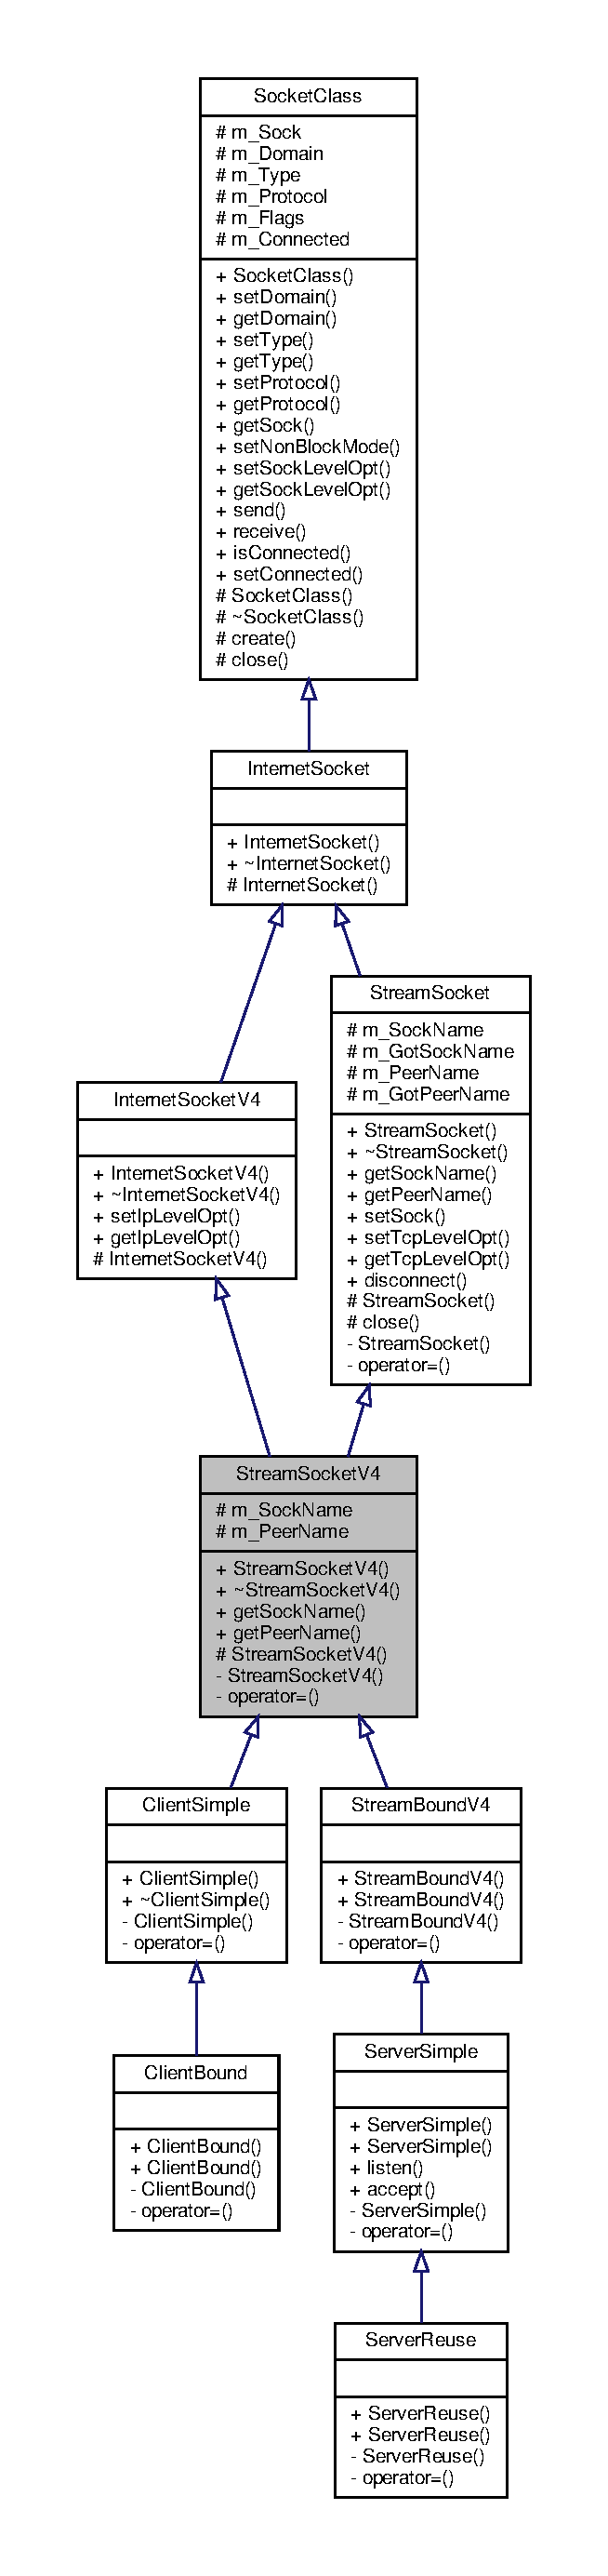
\includegraphics[height=550pt]{classStreamSocketV4__inherit__graph}
\end{center}
\end{figure}
\subsection*{Public Member Functions}
\begin{DoxyCompactItemize}
\item 
\hyperlink{classStreamSocketV4_a00d0a62cc92c6c9a3a29acba866e6483}{Stream\+Socket\+V4} (\hyperlink{sockclasslib_8h_a8dc8083897335125630f1af5dafd5831}{S\+O\+C\+K\+ET} sock)
\item 
virtual \hyperlink{classStreamSocketV4_a6a4b3d769b87c755698b8500942cbdf6}{$\sim$\+Stream\+Socket\+V4} ()
\begin{DoxyCompactList}\small\item\em Destructor. \end{DoxyCompactList}\item 
sockaddr\+\_\+in \& \hyperlink{classStreamSocketV4_ab5edf2c0cbc8b10784ca067cc64bc454}{get\+Sock\+Name} ()
\item 
sockaddr\+\_\+in \& \hyperlink{classStreamSocketV4_ad8ac7763ea0b17c79a9394e22276c2c4}{get\+Peer\+Name} ()
\end{DoxyCompactItemize}
\subsection*{Protected Member Functions}
\begin{DoxyCompactItemize}
\item 
\hyperlink{classStreamSocketV4_ad5ca1c6cb600fa2a247ceae1cd4e7d28}{Stream\+Socket\+V4} ()
\end{DoxyCompactItemize}
\subsection*{Protected Attributes}
\begin{DoxyCompactItemize}
\item 
sockaddr\+\_\+in \hyperlink{classStreamSocketV4_aa90b742744a04670c7533fa219468dc0}{m\+\_\+\+Sock\+Name}
\begin{DoxyCompactList}\small\item\em Bound endpoint properties. \end{DoxyCompactList}\item 
sockaddr\+\_\+in \hyperlink{classStreamSocketV4_a6455bf82f408a10f7e1c7cf0cf1dd535}{m\+\_\+\+Peer\+Name}
\begin{DoxyCompactList}\small\item\em Destination endpoint properties. \end{DoxyCompactList}\end{DoxyCompactItemize}
\subsection*{Private Member Functions}
\begin{DoxyCompactItemize}
\item 
\hyperlink{classStreamSocketV4_a110cb2262536a3882f78c3b7e763bc5d}{Stream\+Socket\+V4} (\hyperlink{classStreamSocketV4}{Stream\+Socket\+V4} \&s)
\item 
\hyperlink{classStreamSocketV4}{Stream\+Socket\+V4} \& \hyperlink{classStreamSocketV4_a4fd37e1d2fd0b358c3a7d9b4e7f4d2e6}{operator=} (\hyperlink{classStreamSocketV4}{Stream\+Socket\+V4} \&s)
\end{DoxyCompactItemize}
\subsection*{Additional Inherited Members}


\subsection{Detailed Description}
Stream socket class for I\+Pv4. The base class for I\+Pv4 stream-\/oriented sockets. 

\subsection{Constructor \& Destructor Documentation}
\mbox{\Hypertarget{classStreamSocketV4_a00d0a62cc92c6c9a3a29acba866e6483}\label{classStreamSocketV4_a00d0a62cc92c6c9a3a29acba866e6483}} 
\index{Stream\+Socket\+V4@{Stream\+Socket\+V4}!Stream\+Socket\+V4@{Stream\+Socket\+V4}}
\index{Stream\+Socket\+V4@{Stream\+Socket\+V4}!Stream\+Socket\+V4@{Stream\+Socket\+V4}}
\subsubsection{\texorpdfstring{Stream\+Socket\+V4()}{StreamSocketV4()}\hspace{0.1cm}{\footnotesize\ttfamily [1/3]}}
{\footnotesize\ttfamily Stream\+Socket\+V4\+::\+Stream\+Socket\+V4 (\begin{DoxyParamCaption}\item[{\hyperlink{sockclasslib_8h_a8dc8083897335125630f1af5dafd5831}{S\+O\+C\+K\+ET}}]{sock }\end{DoxyParamCaption})}

Constructor. 
\begin{DoxyParams}{Parameters}
{\em sock} & \+: socket file descriptor/handle. \\
\hline
\end{DoxyParams}
\mbox{\Hypertarget{classStreamSocketV4_a6a4b3d769b87c755698b8500942cbdf6}\label{classStreamSocketV4_a6a4b3d769b87c755698b8500942cbdf6}} 
\index{Stream\+Socket\+V4@{Stream\+Socket\+V4}!````~Stream\+Socket\+V4@{$\sim$\+Stream\+Socket\+V4}}
\index{````~Stream\+Socket\+V4@{$\sim$\+Stream\+Socket\+V4}!Stream\+Socket\+V4@{Stream\+Socket\+V4}}
\subsubsection{\texorpdfstring{$\sim$\+Stream\+Socket\+V4()}{~StreamSocketV4()}}
{\footnotesize\ttfamily virtual Stream\+Socket\+V4\+::$\sim$\+Stream\+Socket\+V4 (\begin{DoxyParamCaption}{ }\end{DoxyParamCaption})\hspace{0.3cm}{\ttfamily [inline]}, {\ttfamily [virtual]}}



Destructor. 

\mbox{\Hypertarget{classStreamSocketV4_ad5ca1c6cb600fa2a247ceae1cd4e7d28}\label{classStreamSocketV4_ad5ca1c6cb600fa2a247ceae1cd4e7d28}} 
\index{Stream\+Socket\+V4@{Stream\+Socket\+V4}!Stream\+Socket\+V4@{Stream\+Socket\+V4}}
\index{Stream\+Socket\+V4@{Stream\+Socket\+V4}!Stream\+Socket\+V4@{Stream\+Socket\+V4}}
\subsubsection{\texorpdfstring{Stream\+Socket\+V4()}{StreamSocketV4()}\hspace{0.1cm}{\footnotesize\ttfamily [2/3]}}
{\footnotesize\ttfamily Stream\+Socket\+V4\+::\+Stream\+Socket\+V4 (\begin{DoxyParamCaption}{ }\end{DoxyParamCaption})\hspace{0.3cm}{\ttfamily [protected]}}

Constructor. 
\begin{DoxyExceptions}{Exceptions}
{\em Sock\+Exception.} & \\
\hline
\end{DoxyExceptions}
\mbox{\Hypertarget{classStreamSocketV4_a110cb2262536a3882f78c3b7e763bc5d}\label{classStreamSocketV4_a110cb2262536a3882f78c3b7e763bc5d}} 
\index{Stream\+Socket\+V4@{Stream\+Socket\+V4}!Stream\+Socket\+V4@{Stream\+Socket\+V4}}
\index{Stream\+Socket\+V4@{Stream\+Socket\+V4}!Stream\+Socket\+V4@{Stream\+Socket\+V4}}
\subsubsection{\texorpdfstring{Stream\+Socket\+V4()}{StreamSocketV4()}\hspace{0.1cm}{\footnotesize\ttfamily [3/3]}}
{\footnotesize\ttfamily Stream\+Socket\+V4\+::\+Stream\+Socket\+V4 (\begin{DoxyParamCaption}\item[{\hyperlink{classStreamSocketV4}{Stream\+Socket\+V4} \&}]{s }\end{DoxyParamCaption})\hspace{0.3cm}{\ttfamily [private]}}

Constructor. Copy constructor. Makes the class uncopyable. 

\subsection{Member Function Documentation}
\mbox{\Hypertarget{classStreamSocketV4_ad8ac7763ea0b17c79a9394e22276c2c4}\label{classStreamSocketV4_ad8ac7763ea0b17c79a9394e22276c2c4}} 
\index{Stream\+Socket\+V4@{Stream\+Socket\+V4}!get\+Peer\+Name@{get\+Peer\+Name}}
\index{get\+Peer\+Name@{get\+Peer\+Name}!Stream\+Socket\+V4@{Stream\+Socket\+V4}}
\subsubsection{\texorpdfstring{get\+Peer\+Name()}{getPeerName()}}
{\footnotesize\ttfamily sockaddr\+\_\+in \& Stream\+Socket\+V4\+::get\+Peer\+Name (\begin{DoxyParamCaption}{ }\end{DoxyParamCaption})}

Deliver connected endpoint properties. \begin{DoxyReturn}{Returns}
sockaddr\+\_\+in structure filled with connected endpoint properties. 
\end{DoxyReturn}

\begin{DoxyExceptions}{Exceptions}
{\em Sock\+Exception.} & \\
\hline
\end{DoxyExceptions}
\mbox{\Hypertarget{classStreamSocketV4_ab5edf2c0cbc8b10784ca067cc64bc454}\label{classStreamSocketV4_ab5edf2c0cbc8b10784ca067cc64bc454}} 
\index{Stream\+Socket\+V4@{Stream\+Socket\+V4}!get\+Sock\+Name@{get\+Sock\+Name}}
\index{get\+Sock\+Name@{get\+Sock\+Name}!Stream\+Socket\+V4@{Stream\+Socket\+V4}}
\subsubsection{\texorpdfstring{get\+Sock\+Name()}{getSockName()}}
{\footnotesize\ttfamily sockaddr\+\_\+in \& Stream\+Socket\+V4\+::get\+Sock\+Name (\begin{DoxyParamCaption}{ }\end{DoxyParamCaption})}

Deliver bound endpoint properties. \begin{DoxyReturn}{Returns}
sockaddr\+\_\+in structure filled with bound endpoint properties. 
\end{DoxyReturn}

\begin{DoxyExceptions}{Exceptions}
{\em Sock\+Exception.} & \\
\hline
\end{DoxyExceptions}
\mbox{\Hypertarget{classStreamSocketV4_a4fd37e1d2fd0b358c3a7d9b4e7f4d2e6}\label{classStreamSocketV4_a4fd37e1d2fd0b358c3a7d9b4e7f4d2e6}} 
\index{Stream\+Socket\+V4@{Stream\+Socket\+V4}!operator=@{operator=}}
\index{operator=@{operator=}!Stream\+Socket\+V4@{Stream\+Socket\+V4}}
\subsubsection{\texorpdfstring{operator=()}{operator=()}}
{\footnotesize\ttfamily \hyperlink{classStreamSocketV4}{Stream\+Socket\+V4}\& Stream\+Socket\+V4\+::operator= (\begin{DoxyParamCaption}\item[{\hyperlink{classStreamSocketV4}{Stream\+Socket\+V4} \&}]{s }\end{DoxyParamCaption})\hspace{0.3cm}{\ttfamily [private]}}

Operator assign. Makes the class uncopyable. 

\subsection{Member Data Documentation}
\mbox{\Hypertarget{classStreamSocketV4_a6455bf82f408a10f7e1c7cf0cf1dd535}\label{classStreamSocketV4_a6455bf82f408a10f7e1c7cf0cf1dd535}} 
\index{Stream\+Socket\+V4@{Stream\+Socket\+V4}!m\+\_\+\+Peer\+Name@{m\+\_\+\+Peer\+Name}}
\index{m\+\_\+\+Peer\+Name@{m\+\_\+\+Peer\+Name}!Stream\+Socket\+V4@{Stream\+Socket\+V4}}
\subsubsection{\texorpdfstring{m\+\_\+\+Peer\+Name}{m\_PeerName}}
{\footnotesize\ttfamily sockaddr\+\_\+in Stream\+Socket\+V4\+::m\+\_\+\+Peer\+Name\hspace{0.3cm}{\ttfamily [protected]}}



Destination endpoint properties. 

\mbox{\Hypertarget{classStreamSocketV4_aa90b742744a04670c7533fa219468dc0}\label{classStreamSocketV4_aa90b742744a04670c7533fa219468dc0}} 
\index{Stream\+Socket\+V4@{Stream\+Socket\+V4}!m\+\_\+\+Sock\+Name@{m\+\_\+\+Sock\+Name}}
\index{m\+\_\+\+Sock\+Name@{m\+\_\+\+Sock\+Name}!Stream\+Socket\+V4@{Stream\+Socket\+V4}}
\subsubsection{\texorpdfstring{m\+\_\+\+Sock\+Name}{m\_SockName}}
{\footnotesize\ttfamily sockaddr\+\_\+in Stream\+Socket\+V4\+::m\+\_\+\+Sock\+Name\hspace{0.3cm}{\ttfamily [protected]}}



Bound endpoint properties. 



The documentation for this class was generated from the following files\+:\begin{DoxyCompactItemize}
\item 
\hyperlink{StreamSocketV4_8h}{Stream\+Socket\+V4.\+h}\item 
\hyperlink{StreamSocketV4_8cpp}{Stream\+Socket\+V4.\+cpp}\end{DoxyCompactItemize}

\hypertarget{classStreamSocketV6}{}\section{Stream\+Socket\+V6 Class Reference}
\label{classStreamSocketV6}\index{Stream\+Socket\+V6@{Stream\+Socket\+V6}}


{\ttfamily \#include $<$Stream\+Socket\+V6.\+h$>$}



Inheritance diagram for Stream\+Socket\+V6\+:\nopagebreak
\begin{figure}[H]
\begin{center}
\leavevmode
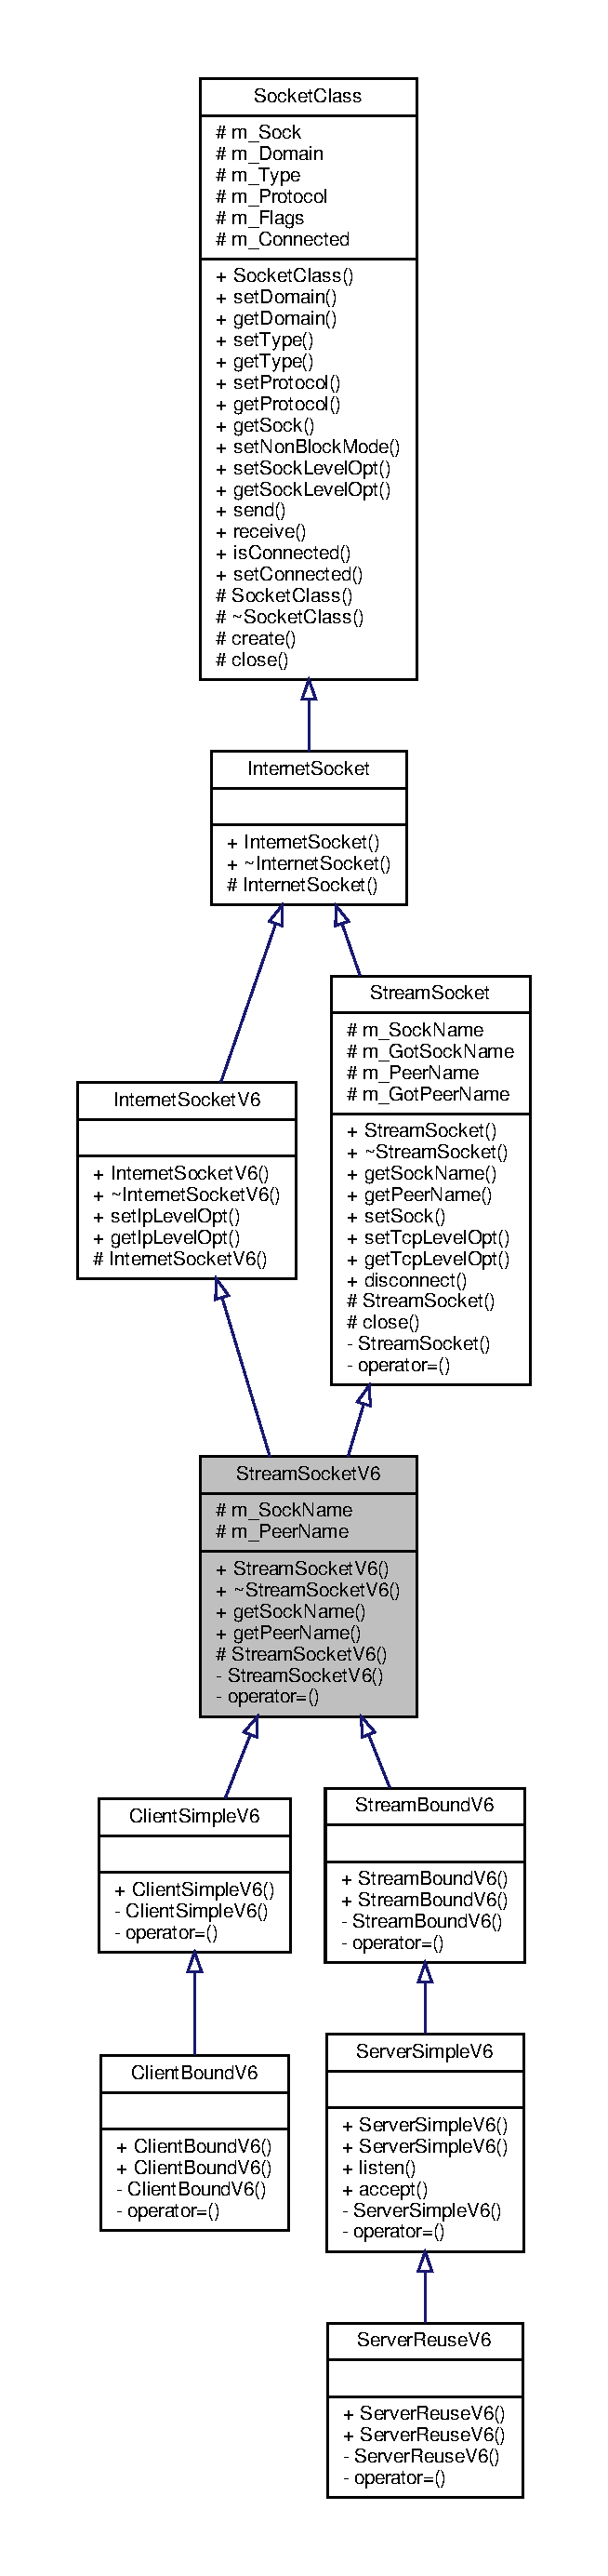
\includegraphics[height=550pt]{classStreamSocketV6__inherit__graph}
\end{center}
\end{figure}
\subsection*{Public Member Functions}
\begin{DoxyCompactItemize}
\item 
\hyperlink{classStreamSocketV6_a5054358161d8ef234de9aa0bdb125b39}{Stream\+Socket\+V6} (\hyperlink{sockclasslib_8h_a8dc8083897335125630f1af5dafd5831}{S\+O\+C\+K\+ET} sock)
\item 
virtual \hyperlink{classStreamSocketV6_a5708fcef318b11a9992f6b0b1861b2ff}{$\sim$\+Stream\+Socket\+V6} ()
\begin{DoxyCompactList}\small\item\em Destructor. \end{DoxyCompactList}\item 
sockaddr\+\_\+in6 \& \hyperlink{classStreamSocketV6_a93f4d15bfc95c567da19372d18e44cf1}{get\+Sock\+Name} ()
\item 
sockaddr\+\_\+in6 \& \hyperlink{classStreamSocketV6_a8ebf6f50686e62c8aa080a2a47d4f82e}{get\+Peer\+Name} ()
\end{DoxyCompactItemize}
\subsection*{Protected Member Functions}
\begin{DoxyCompactItemize}
\item 
\hyperlink{classStreamSocketV6_a0853a7bf3a3d52e4fd0fbed57e2424ef}{Stream\+Socket\+V6} ()
\begin{DoxyCompactList}\small\item\em Constructor. \end{DoxyCompactList}\end{DoxyCompactItemize}
\subsection*{Protected Attributes}
\begin{DoxyCompactItemize}
\item 
sockaddr\+\_\+in6 \hyperlink{classStreamSocketV6_a85f854ff218fbdeb902fd2878fe25526}{m\+\_\+\+Sock\+Name}
\begin{DoxyCompactList}\small\item\em Bound endpoint properties. \end{DoxyCompactList}\item 
sockaddr\+\_\+in6 \hyperlink{classStreamSocketV6_a1817bd2ca5296c8adc8a73234b9ce1cd}{m\+\_\+\+Peer\+Name}
\begin{DoxyCompactList}\small\item\em Destination endpoint properties. \end{DoxyCompactList}\end{DoxyCompactItemize}
\subsection*{Private Member Functions}
\begin{DoxyCompactItemize}
\item 
\hyperlink{classStreamSocketV6_a49ebe7ba5b2e991bd8008d25dd1bd5f3}{Stream\+Socket\+V6} (\hyperlink{classStreamSocketV6}{Stream\+Socket\+V6} \&s)
\item 
\hyperlink{classStreamSocketV6}{Stream\+Socket\+V6} \& \hyperlink{classStreamSocketV6_a4e7ad9f0cfabfe509880ad671636a194}{operator=} (\hyperlink{classStreamSocketV6}{Stream\+Socket\+V6} \&s)
\end{DoxyCompactItemize}
\subsection*{Additional Inherited Members}


\subsection{Detailed Description}
Stream socket class for I\+Pv6. The base class for all stream-\/oriented sockets. 

\subsection{Constructor \& Destructor Documentation}
\mbox{\Hypertarget{classStreamSocketV6_a5054358161d8ef234de9aa0bdb125b39}\label{classStreamSocketV6_a5054358161d8ef234de9aa0bdb125b39}} 
\index{Stream\+Socket\+V6@{Stream\+Socket\+V6}!Stream\+Socket\+V6@{Stream\+Socket\+V6}}
\index{Stream\+Socket\+V6@{Stream\+Socket\+V6}!Stream\+Socket\+V6@{Stream\+Socket\+V6}}
\subsubsection{\texorpdfstring{Stream\+Socket\+V6()}{StreamSocketV6()}\hspace{0.1cm}{\footnotesize\ttfamily [1/3]}}
{\footnotesize\ttfamily Stream\+Socket\+V6\+::\+Stream\+Socket\+V6 (\begin{DoxyParamCaption}\item[{\hyperlink{sockclasslib_8h_a8dc8083897335125630f1af5dafd5831}{S\+O\+C\+K\+ET}}]{sock }\end{DoxyParamCaption})}

Constructor. 
\begin{DoxyParams}{Parameters}
{\em sock} & \+: socket file descriptor/handle. \\
\hline
\end{DoxyParams}
\mbox{\Hypertarget{classStreamSocketV6_a5708fcef318b11a9992f6b0b1861b2ff}\label{classStreamSocketV6_a5708fcef318b11a9992f6b0b1861b2ff}} 
\index{Stream\+Socket\+V6@{Stream\+Socket\+V6}!````~Stream\+Socket\+V6@{$\sim$\+Stream\+Socket\+V6}}
\index{````~Stream\+Socket\+V6@{$\sim$\+Stream\+Socket\+V6}!Stream\+Socket\+V6@{Stream\+Socket\+V6}}
\subsubsection{\texorpdfstring{$\sim$\+Stream\+Socket\+V6()}{~StreamSocketV6()}}
{\footnotesize\ttfamily virtual Stream\+Socket\+V6\+::$\sim$\+Stream\+Socket\+V6 (\begin{DoxyParamCaption}{ }\end{DoxyParamCaption})\hspace{0.3cm}{\ttfamily [inline]}, {\ttfamily [virtual]}}



Destructor. 

\mbox{\Hypertarget{classStreamSocketV6_a0853a7bf3a3d52e4fd0fbed57e2424ef}\label{classStreamSocketV6_a0853a7bf3a3d52e4fd0fbed57e2424ef}} 
\index{Stream\+Socket\+V6@{Stream\+Socket\+V6}!Stream\+Socket\+V6@{Stream\+Socket\+V6}}
\index{Stream\+Socket\+V6@{Stream\+Socket\+V6}!Stream\+Socket\+V6@{Stream\+Socket\+V6}}
\subsubsection{\texorpdfstring{Stream\+Socket\+V6()}{StreamSocketV6()}\hspace{0.1cm}{\footnotesize\ttfamily [2/3]}}
{\footnotesize\ttfamily Stream\+Socket\+V6\+::\+Stream\+Socket\+V6 (\begin{DoxyParamCaption}{ }\end{DoxyParamCaption})\hspace{0.3cm}{\ttfamily [protected]}}



Constructor. 

\mbox{\Hypertarget{classStreamSocketV6_a49ebe7ba5b2e991bd8008d25dd1bd5f3}\label{classStreamSocketV6_a49ebe7ba5b2e991bd8008d25dd1bd5f3}} 
\index{Stream\+Socket\+V6@{Stream\+Socket\+V6}!Stream\+Socket\+V6@{Stream\+Socket\+V6}}
\index{Stream\+Socket\+V6@{Stream\+Socket\+V6}!Stream\+Socket\+V6@{Stream\+Socket\+V6}}
\subsubsection{\texorpdfstring{Stream\+Socket\+V6()}{StreamSocketV6()}\hspace{0.1cm}{\footnotesize\ttfamily [3/3]}}
{\footnotesize\ttfamily Stream\+Socket\+V6\+::\+Stream\+Socket\+V6 (\begin{DoxyParamCaption}\item[{\hyperlink{classStreamSocketV6}{Stream\+Socket\+V6} \&}]{s }\end{DoxyParamCaption})\hspace{0.3cm}{\ttfamily [private]}}

Constructor. Copy constructor. Makes the class uncopyable. 

\subsection{Member Function Documentation}
\mbox{\Hypertarget{classStreamSocketV6_a8ebf6f50686e62c8aa080a2a47d4f82e}\label{classStreamSocketV6_a8ebf6f50686e62c8aa080a2a47d4f82e}} 
\index{Stream\+Socket\+V6@{Stream\+Socket\+V6}!get\+Peer\+Name@{get\+Peer\+Name}}
\index{get\+Peer\+Name@{get\+Peer\+Name}!Stream\+Socket\+V6@{Stream\+Socket\+V6}}
\subsubsection{\texorpdfstring{get\+Peer\+Name()}{getPeerName()}}
{\footnotesize\ttfamily sockaddr\+\_\+in6 \& Stream\+Socket\+V6\+::get\+Peer\+Name (\begin{DoxyParamCaption}{ }\end{DoxyParamCaption})}

Deliver connected endpoint properties. \begin{DoxyReturn}{Returns}
sockaddr\+\_\+in structure filled with connected endpoint properties. 
\end{DoxyReturn}

\begin{DoxyExceptions}{Exceptions}
{\em Sock\+Exception.} & \\
\hline
\end{DoxyExceptions}
\mbox{\Hypertarget{classStreamSocketV6_a93f4d15bfc95c567da19372d18e44cf1}\label{classStreamSocketV6_a93f4d15bfc95c567da19372d18e44cf1}} 
\index{Stream\+Socket\+V6@{Stream\+Socket\+V6}!get\+Sock\+Name@{get\+Sock\+Name}}
\index{get\+Sock\+Name@{get\+Sock\+Name}!Stream\+Socket\+V6@{Stream\+Socket\+V6}}
\subsubsection{\texorpdfstring{get\+Sock\+Name()}{getSockName()}}
{\footnotesize\ttfamily sockaddr\+\_\+in6 \& Stream\+Socket\+V6\+::get\+Sock\+Name (\begin{DoxyParamCaption}{ }\end{DoxyParamCaption})}

Deliver bound endpoint properties. \begin{DoxyReturn}{Returns}
sockaddr\+\_\+in structure filled with bound endpoint properties. 
\end{DoxyReturn}

\begin{DoxyExceptions}{Exceptions}
{\em Sock\+Exception.} & \\
\hline
\end{DoxyExceptions}
\mbox{\Hypertarget{classStreamSocketV6_a4e7ad9f0cfabfe509880ad671636a194}\label{classStreamSocketV6_a4e7ad9f0cfabfe509880ad671636a194}} 
\index{Stream\+Socket\+V6@{Stream\+Socket\+V6}!operator=@{operator=}}
\index{operator=@{operator=}!Stream\+Socket\+V6@{Stream\+Socket\+V6}}
\subsubsection{\texorpdfstring{operator=()}{operator=()}}
{\footnotesize\ttfamily \hyperlink{classStreamSocketV6}{Stream\+Socket\+V6}\& Stream\+Socket\+V6\+::operator= (\begin{DoxyParamCaption}\item[{\hyperlink{classStreamSocketV6}{Stream\+Socket\+V6} \&}]{s }\end{DoxyParamCaption})\hspace{0.3cm}{\ttfamily [private]}}

Operator assign. Makes the class uncopyable. 

\subsection{Member Data Documentation}
\mbox{\Hypertarget{classStreamSocketV6_a1817bd2ca5296c8adc8a73234b9ce1cd}\label{classStreamSocketV6_a1817bd2ca5296c8adc8a73234b9ce1cd}} 
\index{Stream\+Socket\+V6@{Stream\+Socket\+V6}!m\+\_\+\+Peer\+Name@{m\+\_\+\+Peer\+Name}}
\index{m\+\_\+\+Peer\+Name@{m\+\_\+\+Peer\+Name}!Stream\+Socket\+V6@{Stream\+Socket\+V6}}
\subsubsection{\texorpdfstring{m\+\_\+\+Peer\+Name}{m\_PeerName}}
{\footnotesize\ttfamily sockaddr\+\_\+in6 Stream\+Socket\+V6\+::m\+\_\+\+Peer\+Name\hspace{0.3cm}{\ttfamily [protected]}}



Destination endpoint properties. 

\mbox{\Hypertarget{classStreamSocketV6_a85f854ff218fbdeb902fd2878fe25526}\label{classStreamSocketV6_a85f854ff218fbdeb902fd2878fe25526}} 
\index{Stream\+Socket\+V6@{Stream\+Socket\+V6}!m\+\_\+\+Sock\+Name@{m\+\_\+\+Sock\+Name}}
\index{m\+\_\+\+Sock\+Name@{m\+\_\+\+Sock\+Name}!Stream\+Socket\+V6@{Stream\+Socket\+V6}}
\subsubsection{\texorpdfstring{m\+\_\+\+Sock\+Name}{m\_SockName}}
{\footnotesize\ttfamily sockaddr\+\_\+in6 Stream\+Socket\+V6\+::m\+\_\+\+Sock\+Name\hspace{0.3cm}{\ttfamily [protected]}}



Bound endpoint properties. 



The documentation for this class was generated from the following files\+:\begin{DoxyCompactItemize}
\item 
\hyperlink{StreamSocketV6_8h}{Stream\+Socket\+V6.\+h}\item 
\hyperlink{StreamSocketV6_8cpp}{Stream\+Socket\+V6.\+cpp}\end{DoxyCompactItemize}

\hypertarget{structSockClassLib_1_1VersionTriple}{}\section{Sock\+Class\+Lib\+:\+:Version\+Triple Struct Reference}
\label{structSockClassLib_1_1VersionTriple}\index{Sock\+Class\+Lib\+::\+Version\+Triple@{Sock\+Class\+Lib\+::\+Version\+Triple}}


Structure for library versions.  




{\ttfamily \#include $<$sockclasslib.\+h$>$}

\subsection*{Public Attributes}
\begin{DoxyCompactItemize}
\item 
int \hyperlink{structSockClassLib_1_1VersionTriple_a79ce564464e6d4e6fca3d7fc51b42bdd}{Major}
\begin{DoxyCompactList}\small\item\em Major version number. \end{DoxyCompactList}\item 
int \hyperlink{structSockClassLib_1_1VersionTriple_a4588deee7b7e148775da4407af465b8f}{Minor}
\begin{DoxyCompactList}\small\item\em Minor version number. \end{DoxyCompactList}\item 
int \hyperlink{structSockClassLib_1_1VersionTriple_a5ca64bcae906bbd9a629c905548dd845}{Sub\+Minor}
\begin{DoxyCompactList}\small\item\em Minor subversion number. \end{DoxyCompactList}\end{DoxyCompactItemize}


\subsection{Detailed Description}
Structure for library versions. 

\subsection{Member Data Documentation}
\mbox{\Hypertarget{structSockClassLib_1_1VersionTriple_a79ce564464e6d4e6fca3d7fc51b42bdd}\label{structSockClassLib_1_1VersionTriple_a79ce564464e6d4e6fca3d7fc51b42bdd}} 
\index{Sock\+Class\+Lib\+::\+Version\+Triple@{Sock\+Class\+Lib\+::\+Version\+Triple}!Major@{Major}}
\index{Major@{Major}!Sock\+Class\+Lib\+::\+Version\+Triple@{Sock\+Class\+Lib\+::\+Version\+Triple}}
\subsubsection{\texorpdfstring{Major}{Major}}
{\footnotesize\ttfamily int Sock\+Class\+Lib\+::\+Version\+Triple\+::\+Major}



Major version number. 

\mbox{\Hypertarget{structSockClassLib_1_1VersionTriple_a4588deee7b7e148775da4407af465b8f}\label{structSockClassLib_1_1VersionTriple_a4588deee7b7e148775da4407af465b8f}} 
\index{Sock\+Class\+Lib\+::\+Version\+Triple@{Sock\+Class\+Lib\+::\+Version\+Triple}!Minor@{Minor}}
\index{Minor@{Minor}!Sock\+Class\+Lib\+::\+Version\+Triple@{Sock\+Class\+Lib\+::\+Version\+Triple}}
\subsubsection{\texorpdfstring{Minor}{Minor}}
{\footnotesize\ttfamily int Sock\+Class\+Lib\+::\+Version\+Triple\+::\+Minor}



Minor version number. 

\mbox{\Hypertarget{structSockClassLib_1_1VersionTriple_a5ca64bcae906bbd9a629c905548dd845}\label{structSockClassLib_1_1VersionTriple_a5ca64bcae906bbd9a629c905548dd845}} 
\index{Sock\+Class\+Lib\+::\+Version\+Triple@{Sock\+Class\+Lib\+::\+Version\+Triple}!Sub\+Minor@{Sub\+Minor}}
\index{Sub\+Minor@{Sub\+Minor}!Sock\+Class\+Lib\+::\+Version\+Triple@{Sock\+Class\+Lib\+::\+Version\+Triple}}
\subsubsection{\texorpdfstring{Sub\+Minor}{SubMinor}}
{\footnotesize\ttfamily int Sock\+Class\+Lib\+::\+Version\+Triple\+::\+Sub\+Minor}



Minor subversion number. 



The documentation for this struct was generated from the following file\+:\begin{DoxyCompactItemize}
\item 
\hyperlink{sockclasslib_8h}{sockclasslib.\+h}\end{DoxyCompactItemize}

\chapter{File Documentation}
\hypertarget{BaseException_8h}{}\section{Base\+Exception.\+h File Reference}
\label{BaseException_8h}\index{Base\+Exception.\+h@{Base\+Exception.\+h}}
{\ttfamily \#include $<$string.\+h$>$}\newline
{\ttfamily \#include $<$vector$>$}\newline
{\ttfamily \#include $<$strstream$>$}\newline
{\ttfamily \#include $<$string$>$}\newline
{\ttfamily \#include $<$sockclasslib.\+h$>$}\newline
Include dependency graph for Base\+Exception.\+h\+:\nopagebreak
\begin{figure}[H]
\begin{center}
\leavevmode
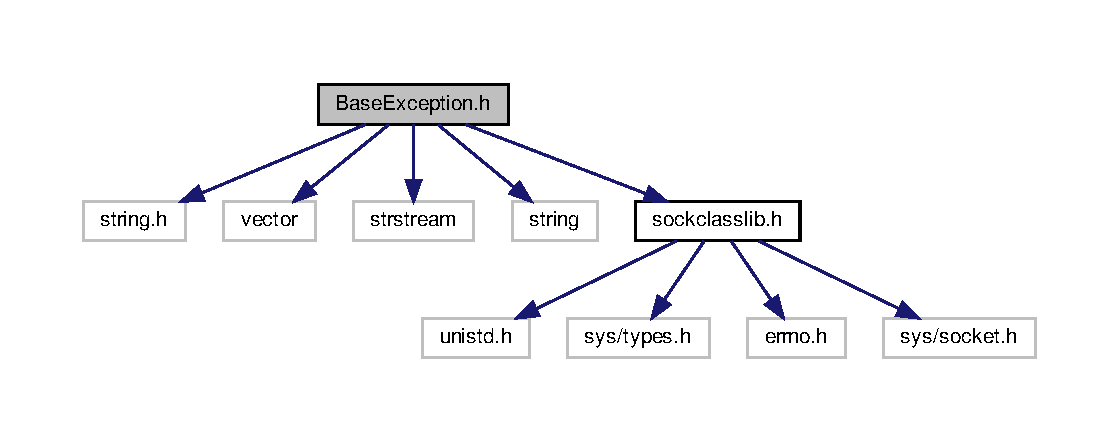
\includegraphics[width=350pt]{BaseException_8h__incl}
\end{center}
\end{figure}
This graph shows which files directly or indirectly include this file\+:\nopagebreak
\begin{figure}[H]
\begin{center}
\leavevmode
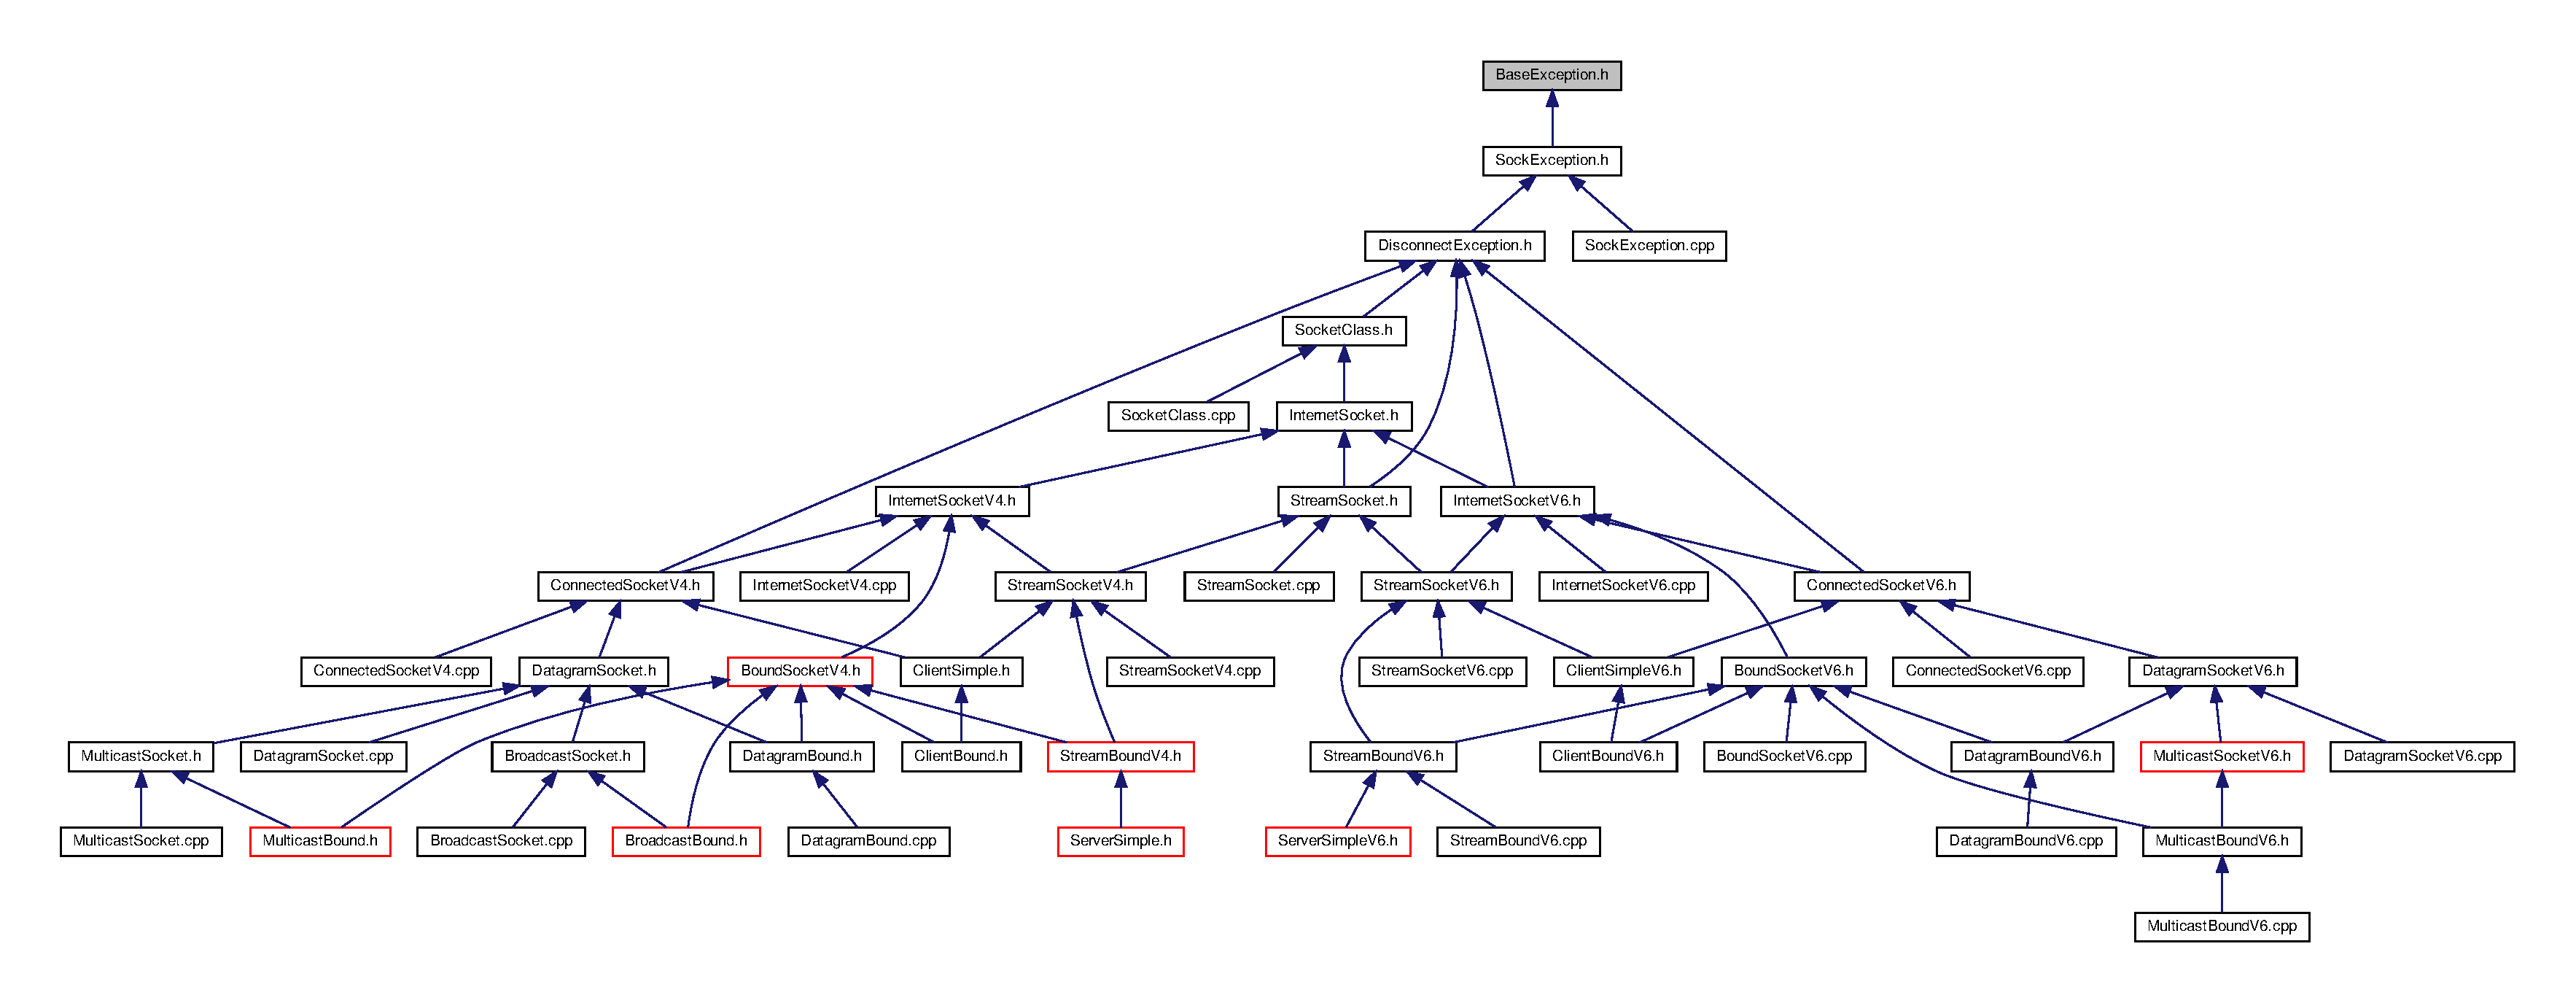
\includegraphics[width=350pt]{BaseException_8h__dep__incl}
\end{center}
\end{figure}
\subsection*{Classes}
\begin{DoxyCompactItemize}
\item 
class \hyperlink{classBaseException}{Base\+Exception}
\end{DoxyCompactItemize}
\subsection*{Macros}
\begin{DoxyCompactItemize}
\item 
\#define \hyperlink{BaseException_8h_adbba0f726fc66d7100916c683b7568ae}{G\+C\+C\+\_\+\+V\+E\+R\+S\+I\+ON}~(\+\_\+\+\_\+\+G\+N\+U\+C\+\_\+\+\_\+ $\ast$ 1000 + \+\_\+\+\_\+\+G\+N\+U\+C\+\_\+\+M\+I\+N\+O\+R\+\_\+\+\_\+)
\begin{DoxyCompactList}\small\item\em G\+C\+C\+\_\+\+V\+E\+R\+S\+I\+ON. \end{DoxyCompactList}\item 
\#define \hyperlink{BaseException_8h_a8d1758336cf46c234f248f3002d1c106}{repstream}~strstream
\begin{DoxyCompactList}\small\item\em repstream \end{DoxyCompactList}\item 
\#define \hyperlink{group__EXCEPT__GROUP_gad17cc7779410e71d94722126b762a3f3}{E\+X\+C\+E\+P\+T\+I\+O\+N\+\_\+\+P\+A\+R\+A\+MS}~\+\_\+\+\_\+\+F\+I\+L\+E\+\_\+\+\_\+, \+\_\+\+\_\+\+L\+I\+N\+E\+\_\+\+\_\+
\begin{DoxyCompactList}\small\item\em Exception parameters includes filename and line number. \end{DoxyCompactList}\end{DoxyCompactItemize}


\subsection{Macro Definition Documentation}
\mbox{\Hypertarget{BaseException_8h_adbba0f726fc66d7100916c683b7568ae}\label{BaseException_8h_adbba0f726fc66d7100916c683b7568ae}} 
\index{Base\+Exception.\+h@{Base\+Exception.\+h}!G\+C\+C\+\_\+\+V\+E\+R\+S\+I\+ON@{G\+C\+C\+\_\+\+V\+E\+R\+S\+I\+ON}}
\index{G\+C\+C\+\_\+\+V\+E\+R\+S\+I\+ON@{G\+C\+C\+\_\+\+V\+E\+R\+S\+I\+ON}!Base\+Exception.\+h@{Base\+Exception.\+h}}
\subsubsection{\texorpdfstring{G\+C\+C\+\_\+\+V\+E\+R\+S\+I\+ON}{GCC\_VERSION}}
{\footnotesize\ttfamily \#define G\+C\+C\+\_\+\+V\+E\+R\+S\+I\+ON~(\+\_\+\+\_\+\+G\+N\+U\+C\+\_\+\+\_\+ $\ast$ 1000 + \+\_\+\+\_\+\+G\+N\+U\+C\+\_\+\+M\+I\+N\+O\+R\+\_\+\+\_\+)}



G\+C\+C\+\_\+\+V\+E\+R\+S\+I\+ON. 

\mbox{\Hypertarget{BaseException_8h_a8d1758336cf46c234f248f3002d1c106}\label{BaseException_8h_a8d1758336cf46c234f248f3002d1c106}} 
\index{Base\+Exception.\+h@{Base\+Exception.\+h}!repstream@{repstream}}
\index{repstream@{repstream}!Base\+Exception.\+h@{Base\+Exception.\+h}}
\subsubsection{\texorpdfstring{repstream}{repstream}}
{\footnotesize\ttfamily \#define repstream~strstream}



repstream 


\hypertarget{BoundSocketV4_8cpp}{}\section{Bound\+Socket\+V4.\+cpp File Reference}
\label{BoundSocketV4_8cpp}\index{Bound\+Socket\+V4.\+cpp@{Bound\+Socket\+V4.\+cpp}}
{\ttfamily \#include $<$Bound\+Socket\+V4.\+h$>$}\newline
Include dependency graph for Bound\+Socket\+V4.\+cpp\+:\nopagebreak
\begin{figure}[H]
\begin{center}
\leavevmode
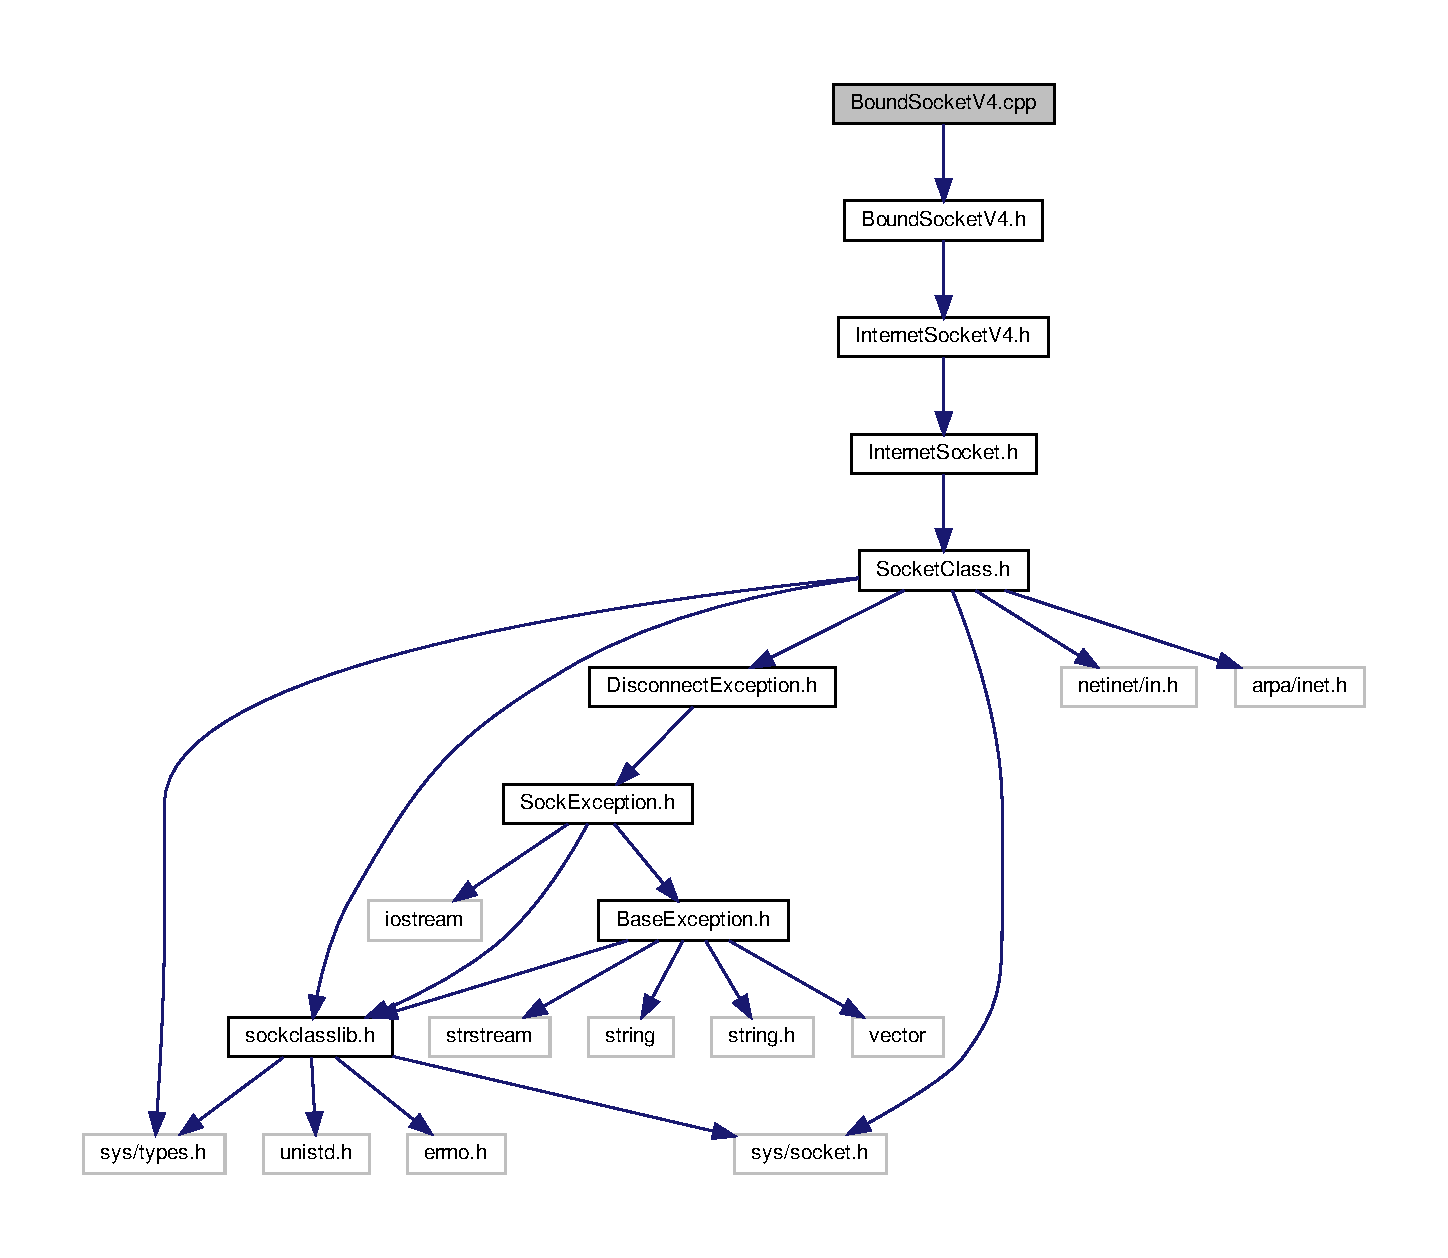
\includegraphics[width=350pt]{BoundSocketV4_8cpp__incl}
\end{center}
\end{figure}

\hypertarget{BoundSocketV4_8h}{}\section{Bound\+Socket\+V4.\+h File Reference}
\label{BoundSocketV4_8h}\index{Bound\+Socket\+V4.\+h@{Bound\+Socket\+V4.\+h}}
{\ttfamily \#include $<$Internet\+Socket\+V4.\+h$>$}\newline
Include dependency graph for Bound\+Socket\+V4.\+h\+:\nopagebreak
\begin{figure}[H]
\begin{center}
\leavevmode
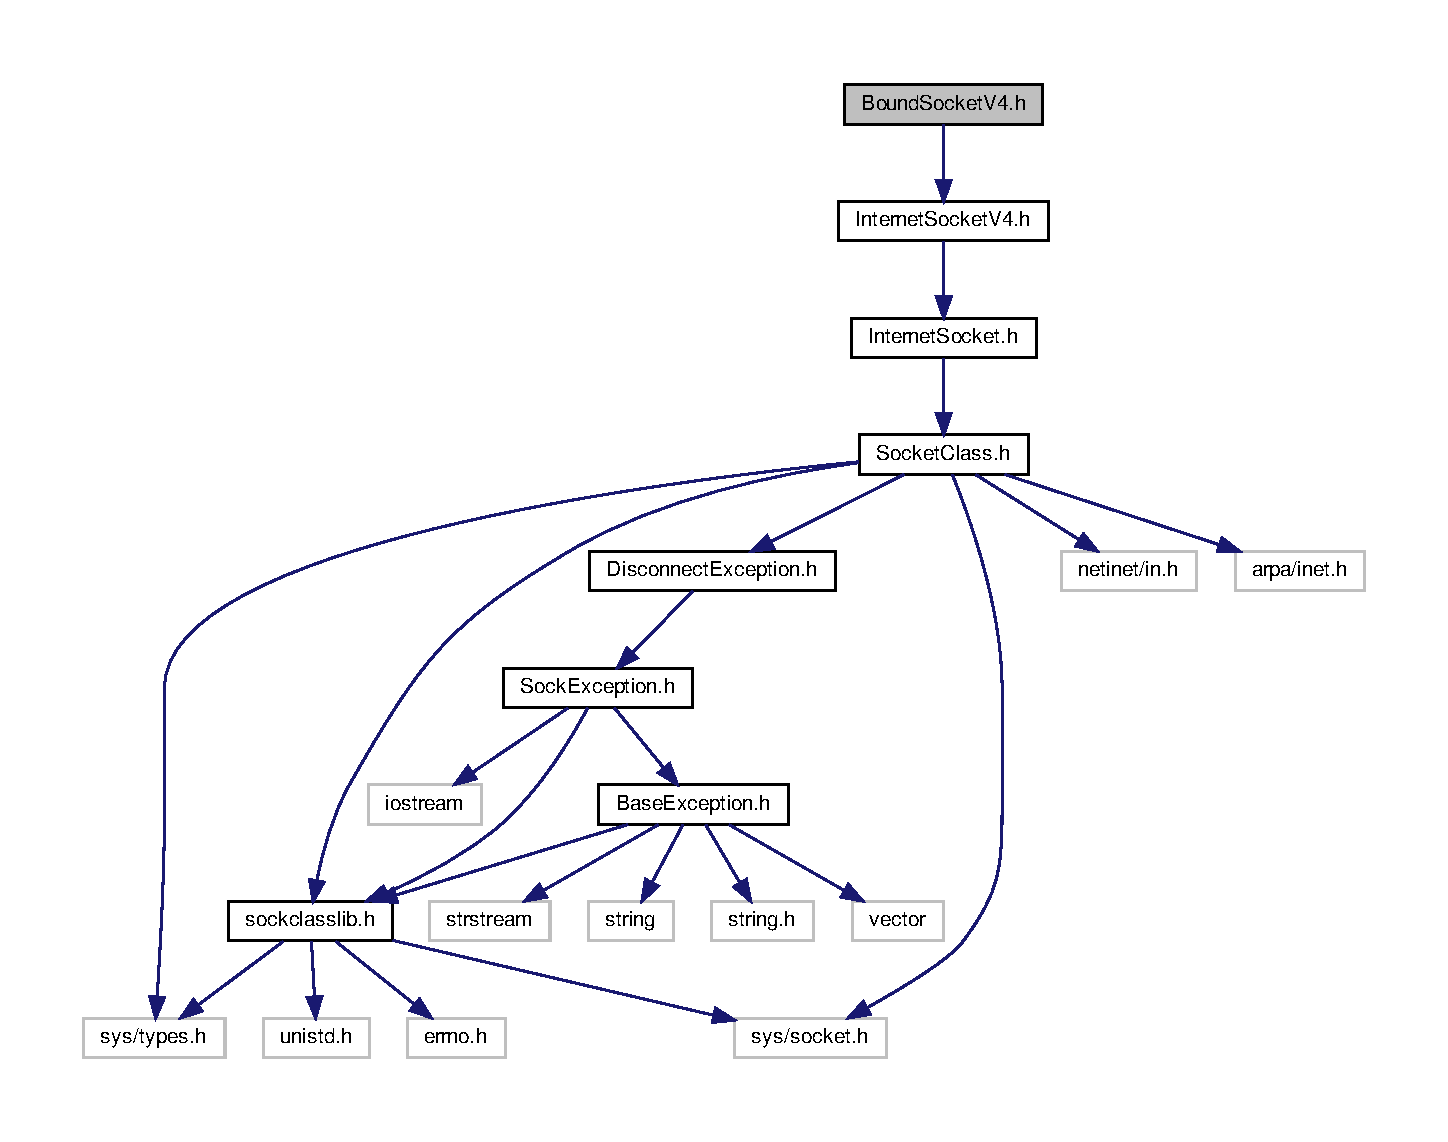
\includegraphics[width=350pt]{BoundSocketV4_8h__incl}
\end{center}
\end{figure}
This graph shows which files directly or indirectly include this file\+:\nopagebreak
\begin{figure}[H]
\begin{center}
\leavevmode
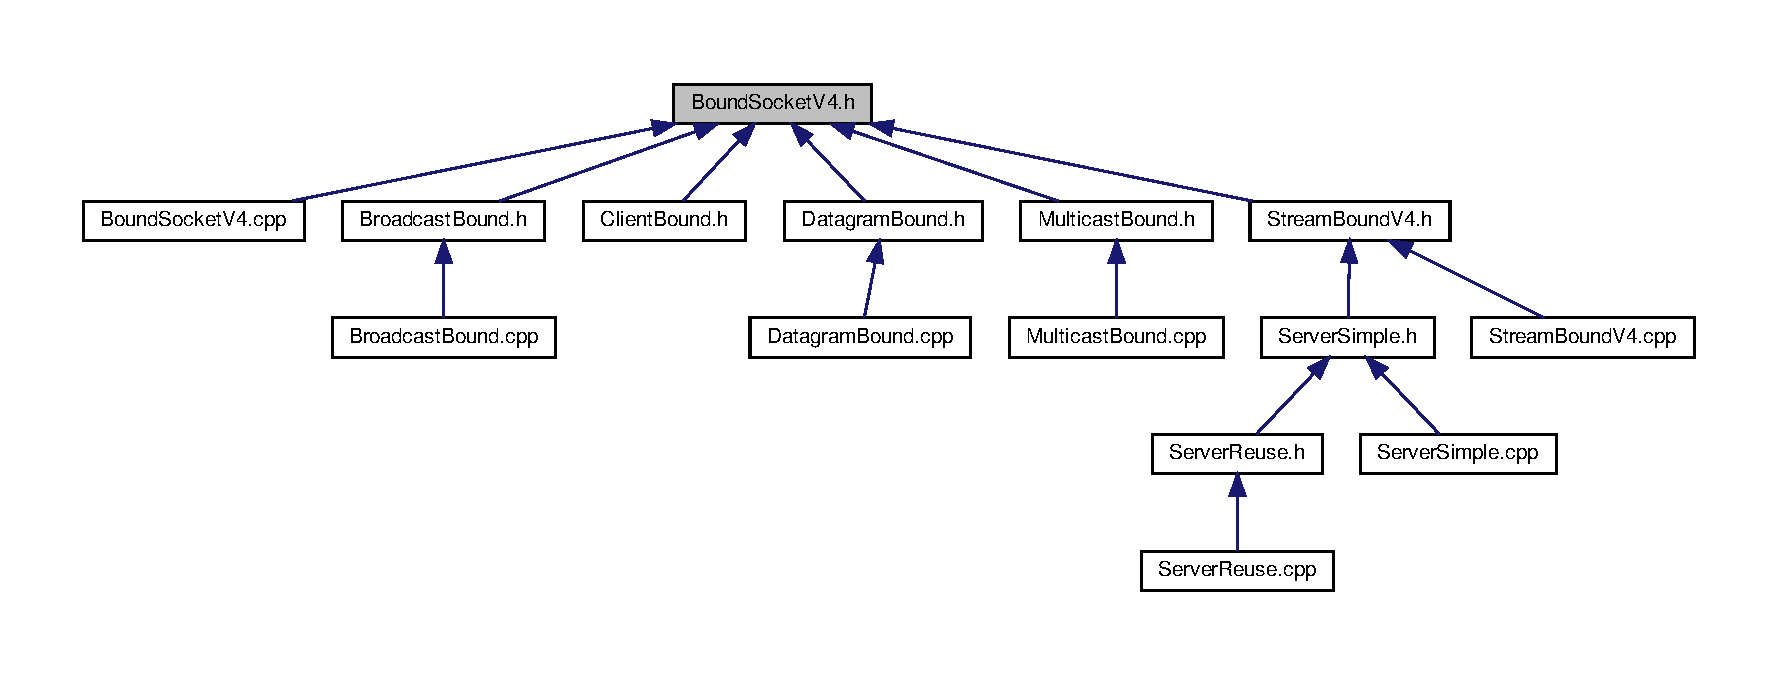
\includegraphics[width=350pt]{BoundSocketV4_8h__dep__incl}
\end{center}
\end{figure}
\subsection*{Classes}
\begin{DoxyCompactItemize}
\item 
class \hyperlink{classBoundSocketV4}{Bound\+Socket\+V4}
\begin{DoxyCompactList}\small\item\em Socket bounded to particular port and I\+Pv4 address (end-\/point). \end{DoxyCompactList}\end{DoxyCompactItemize}

\hypertarget{BoundSocketV6_8cpp}{}\section{Bound\+Socket\+V6.\+cpp File Reference}
\label{BoundSocketV6_8cpp}\index{Bound\+Socket\+V6.\+cpp@{Bound\+Socket\+V6.\+cpp}}
{\ttfamily \#include $<$Bound\+Socket\+V6.\+h$>$}\newline
Include dependency graph for Bound\+Socket\+V6.\+cpp\+:\nopagebreak
\begin{figure}[H]
\begin{center}
\leavevmode
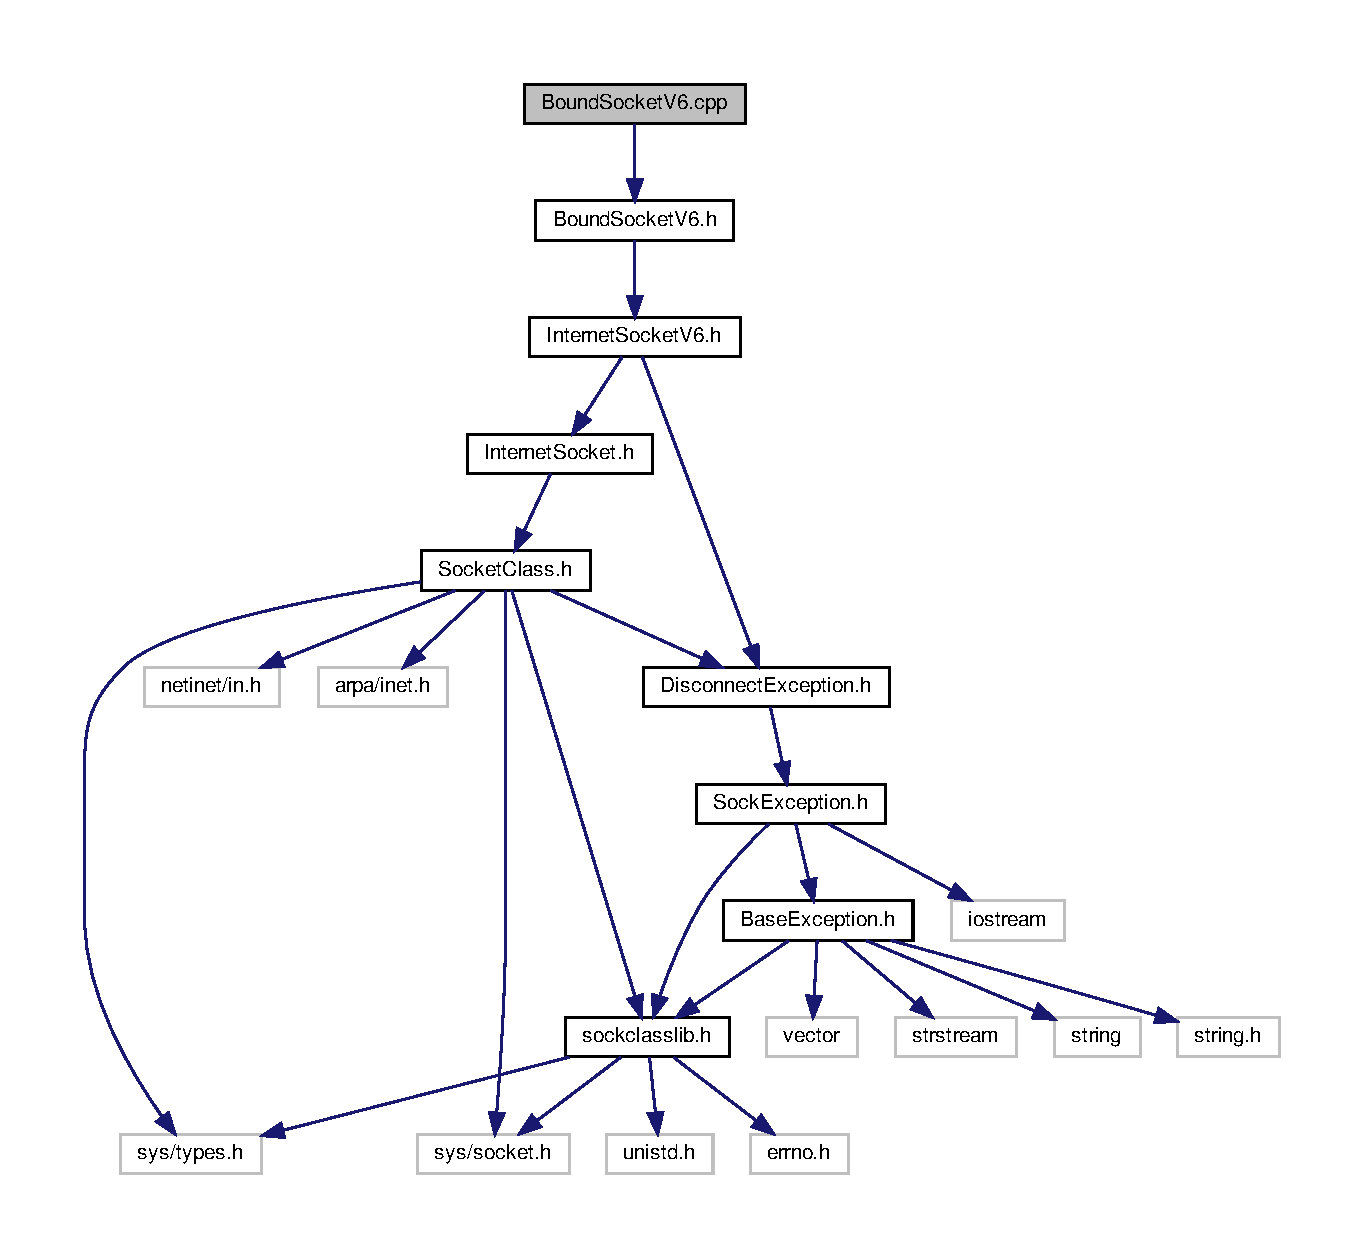
\includegraphics[width=350pt]{BoundSocketV6_8cpp__incl}
\end{center}
\end{figure}

\hypertarget{BoundSocketV6_8h}{}\section{Bound\+Socket\+V6.\+h File Reference}
\label{BoundSocketV6_8h}\index{Bound\+Socket\+V6.\+h@{Bound\+Socket\+V6.\+h}}
{\ttfamily \#include $<$Internet\+Socket\+V6.\+h$>$}\newline
Include dependency graph for Bound\+Socket\+V6.\+h\+:\nopagebreak
\begin{figure}[H]
\begin{center}
\leavevmode
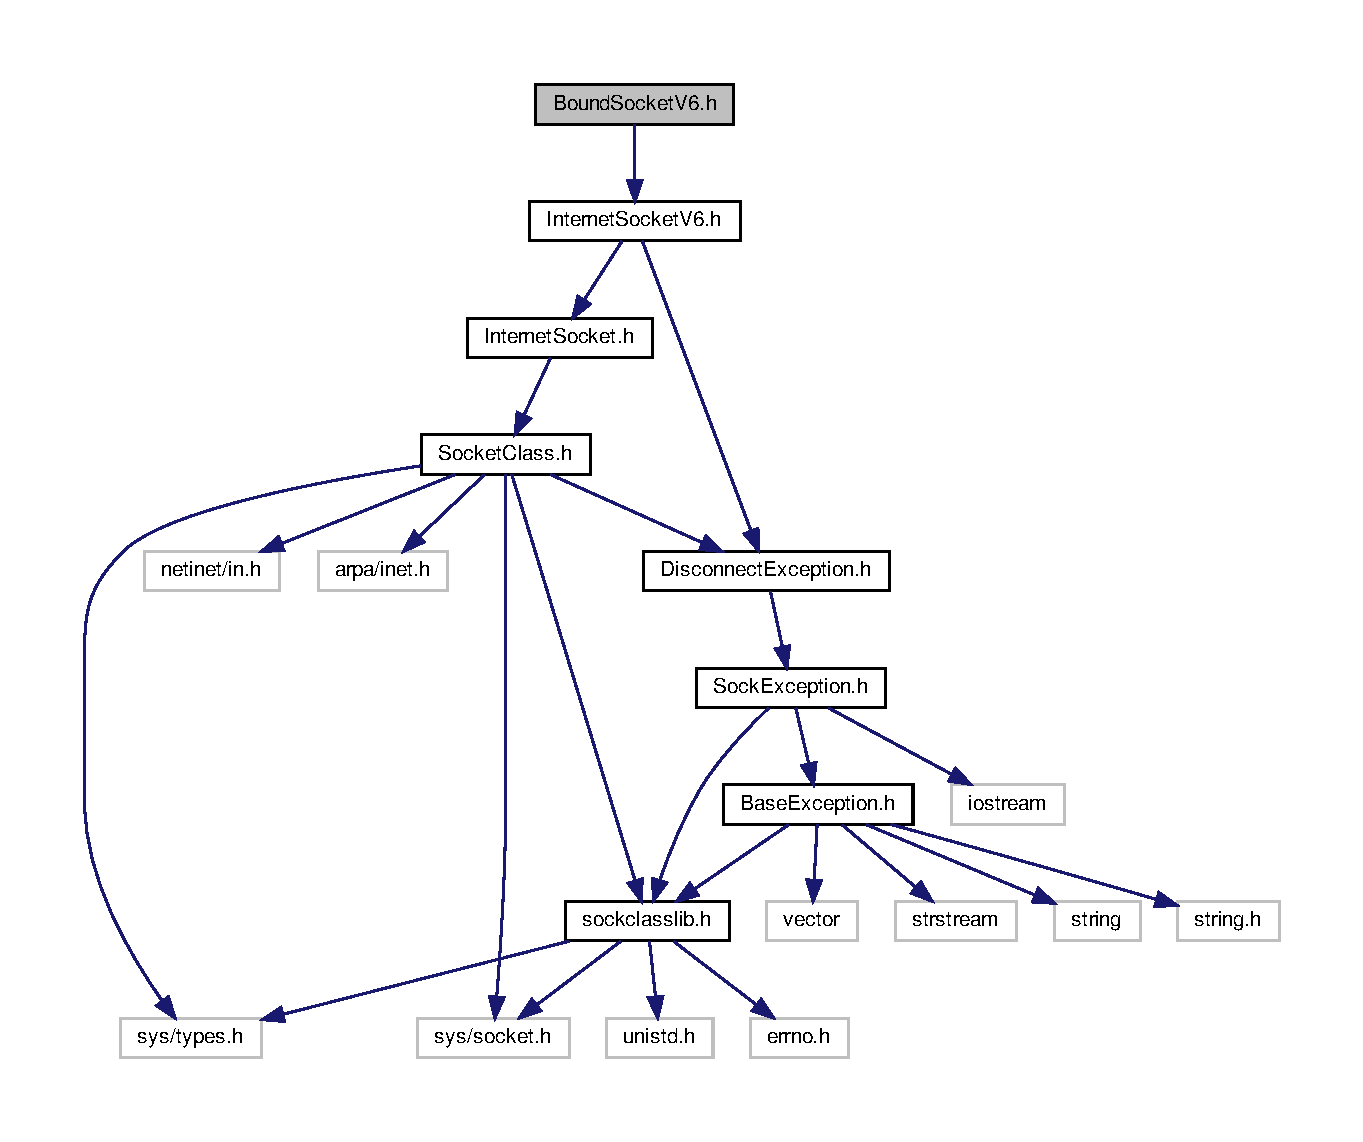
\includegraphics[width=350pt]{BoundSocketV6_8h__incl}
\end{center}
\end{figure}
This graph shows which files directly or indirectly include this file\+:\nopagebreak
\begin{figure}[H]
\begin{center}
\leavevmode
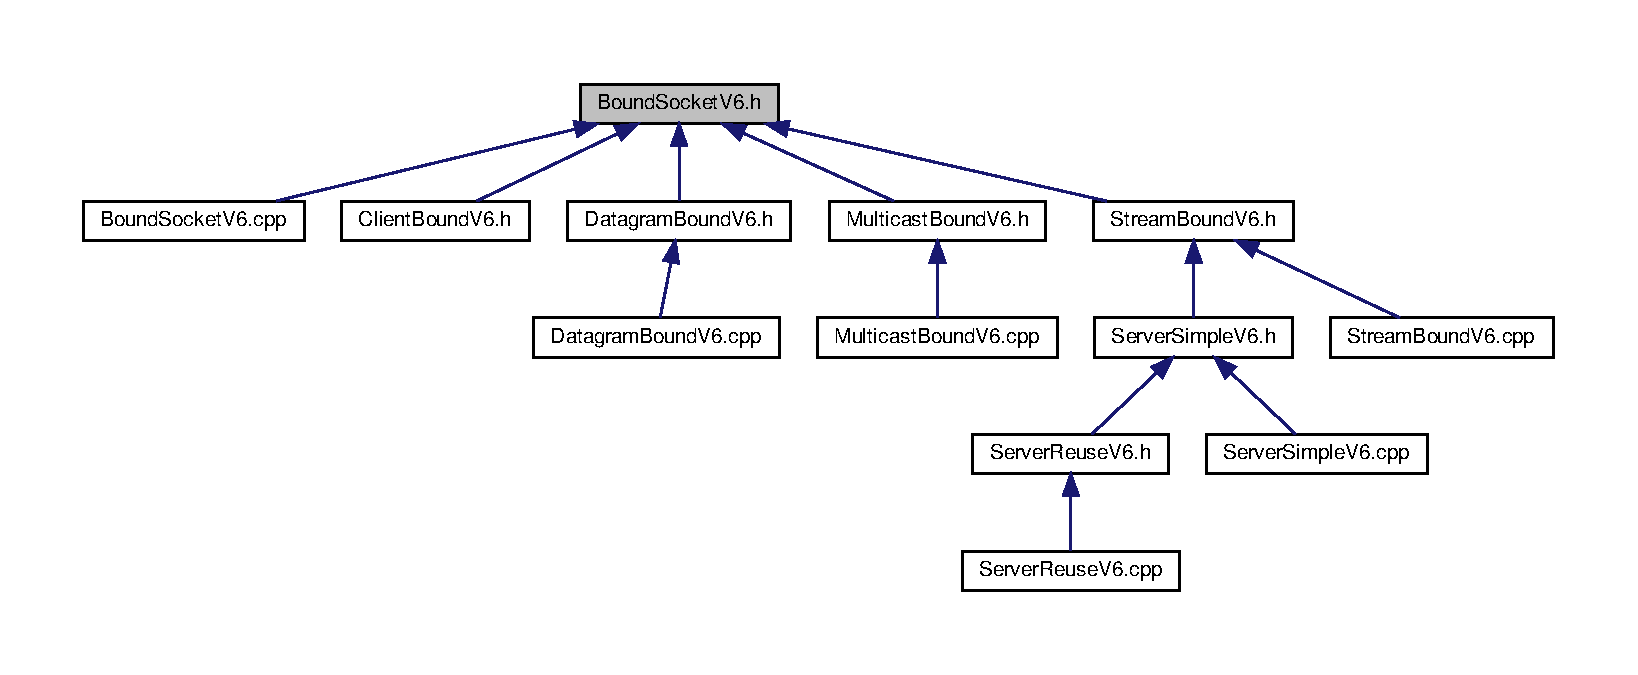
\includegraphics[width=350pt]{BoundSocketV6_8h__dep__incl}
\end{center}
\end{figure}
\subsection*{Classes}
\begin{DoxyCompactItemize}
\item 
class \hyperlink{classBoundSocketV6}{Bound\+Socket\+V6}
\begin{DoxyCompactList}\small\item\em Socket bounded to particular port and I\+Pv6 address (end-\/point). \end{DoxyCompactList}\end{DoxyCompactItemize}

\hypertarget{BroadcastBound_8cpp}{}\section{Broadcast\+Bound.\+cpp File Reference}
\label{BroadcastBound_8cpp}\index{Broadcast\+Bound.\+cpp@{Broadcast\+Bound.\+cpp}}
{\ttfamily \#include $<$Broadcast\+Bound.\+h$>$}\newline
Include dependency graph for Broadcast\+Bound.\+cpp\+:\nopagebreak
\begin{figure}[H]
\begin{center}
\leavevmode
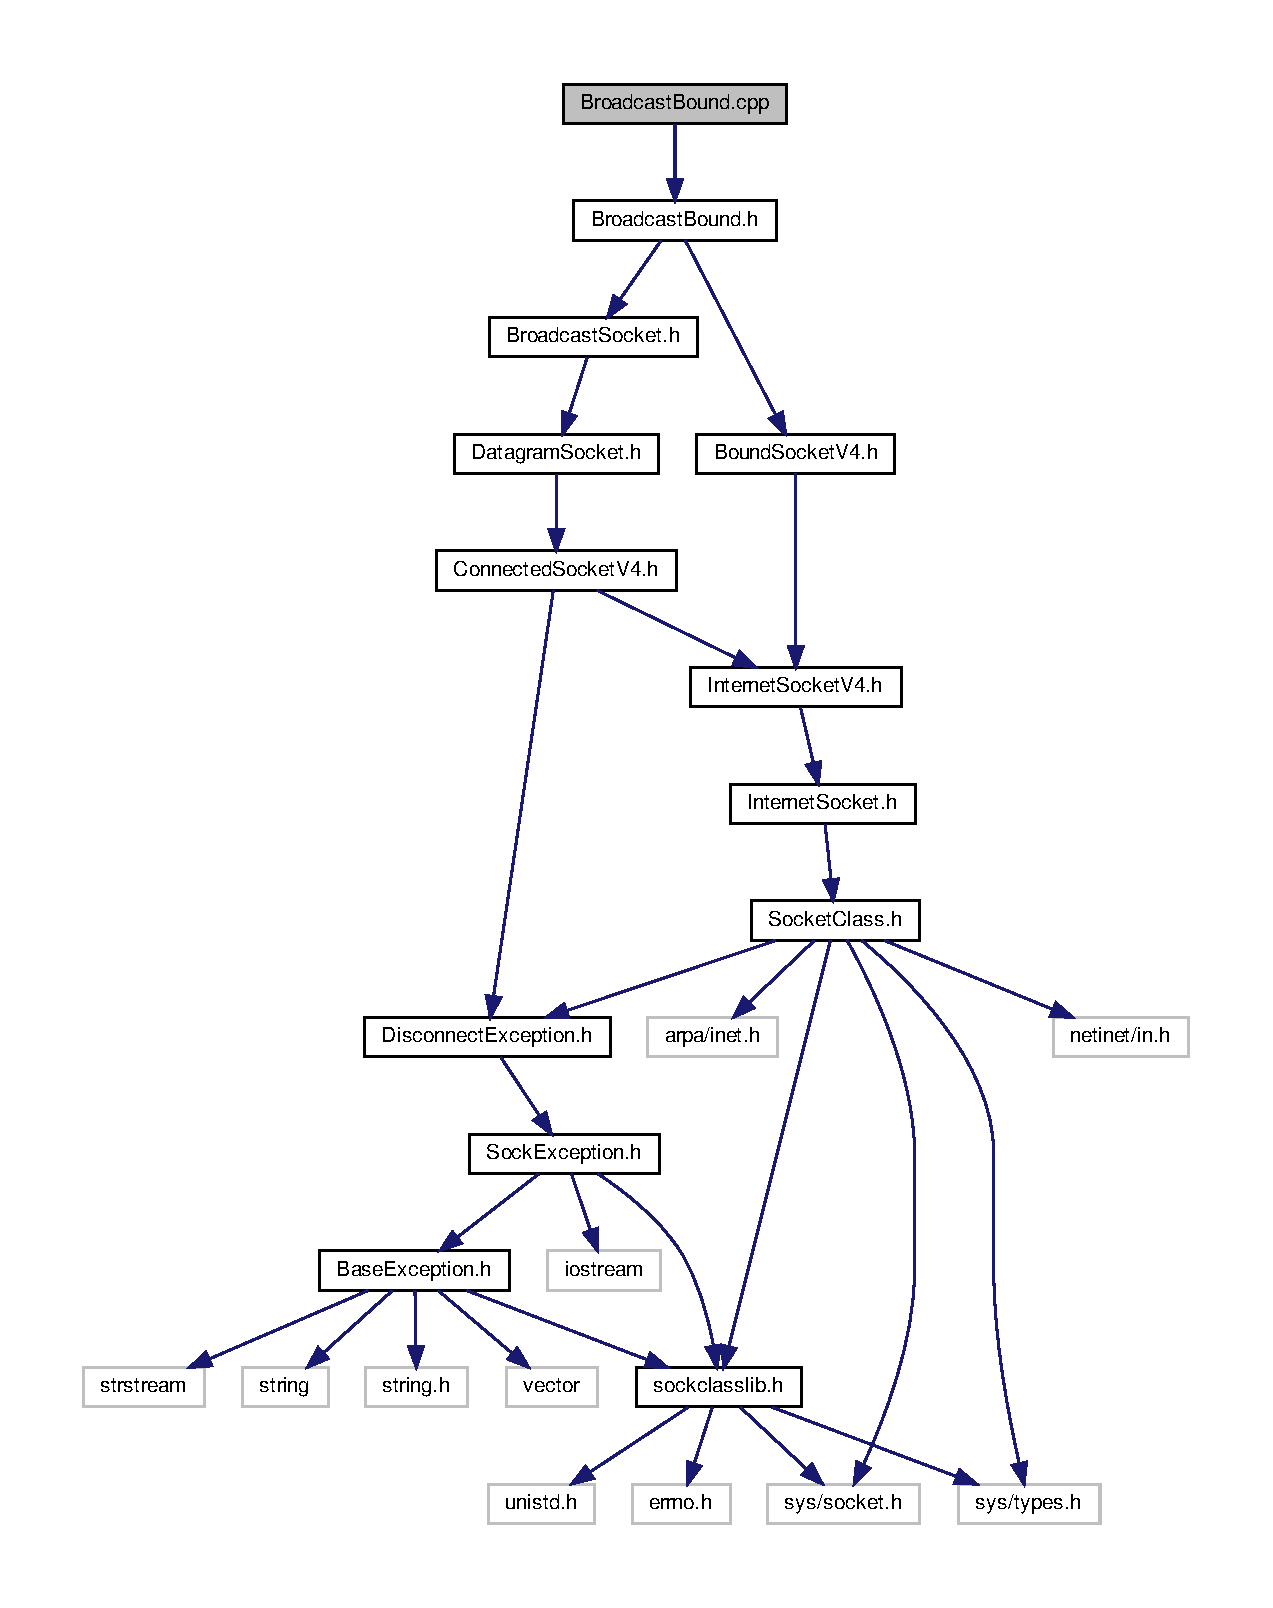
\includegraphics[width=350pt]{BroadcastBound_8cpp__incl}
\end{center}
\end{figure}

\hypertarget{BroadcastBound_8h}{}\section{Broadcast\+Bound.\+h File Reference}
\label{BroadcastBound_8h}\index{Broadcast\+Bound.\+h@{Broadcast\+Bound.\+h}}
{\ttfamily \#include $<$Broadcast\+Socket.\+h$>$}\newline
{\ttfamily \#include $<$Bound\+Socket\+V4.\+h$>$}\newline
Include dependency graph for Broadcast\+Bound.\+h\+:\nopagebreak
\begin{figure}[H]
\begin{center}
\leavevmode
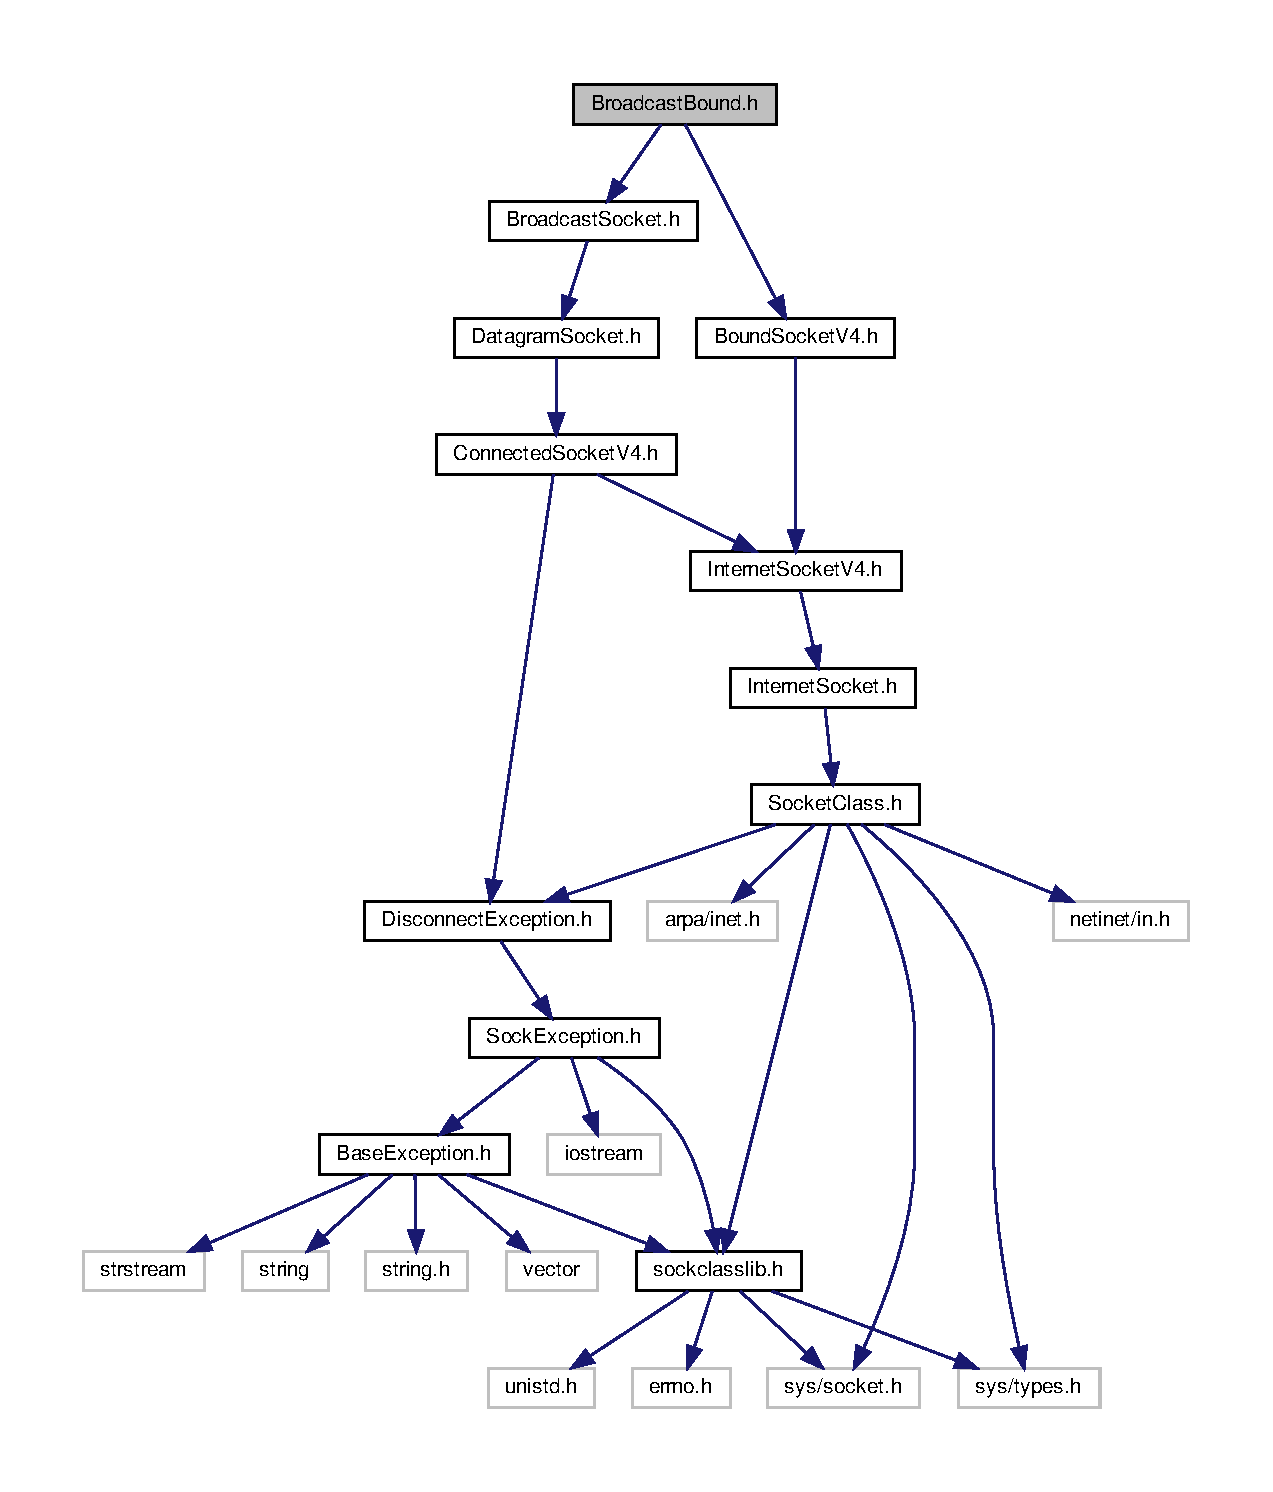
\includegraphics[width=350pt]{BroadcastBound_8h__incl}
\end{center}
\end{figure}
This graph shows which files directly or indirectly include this file\+:\nopagebreak
\begin{figure}[H]
\begin{center}
\leavevmode
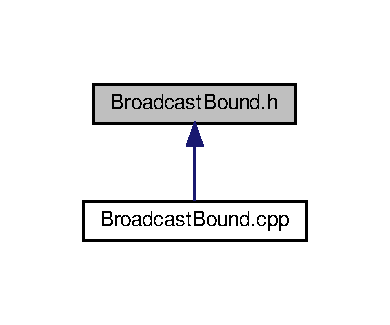
\includegraphics[width=187pt]{BroadcastBound_8h__dep__incl}
\end{center}
\end{figure}
\subsection*{Classes}
\begin{DoxyCompactItemize}
\item 
class \hyperlink{classBroadcastBound}{Broadcast\+Bound}
\begin{DoxyCompactList}\small\item\em Bounded socket with broadcast capabilities. \end{DoxyCompactList}\end{DoxyCompactItemize}

\hypertarget{BroadcastSocket_8cpp}{}\section{Broadcast\+Socket.\+cpp File Reference}
\label{BroadcastSocket_8cpp}\index{Broadcast\+Socket.\+cpp@{Broadcast\+Socket.\+cpp}}
{\ttfamily \#include $<$Broadcast\+Socket.\+h$>$}\newline
Include dependency graph for Broadcast\+Socket.\+cpp\+:\nopagebreak
\begin{figure}[H]
\begin{center}
\leavevmode
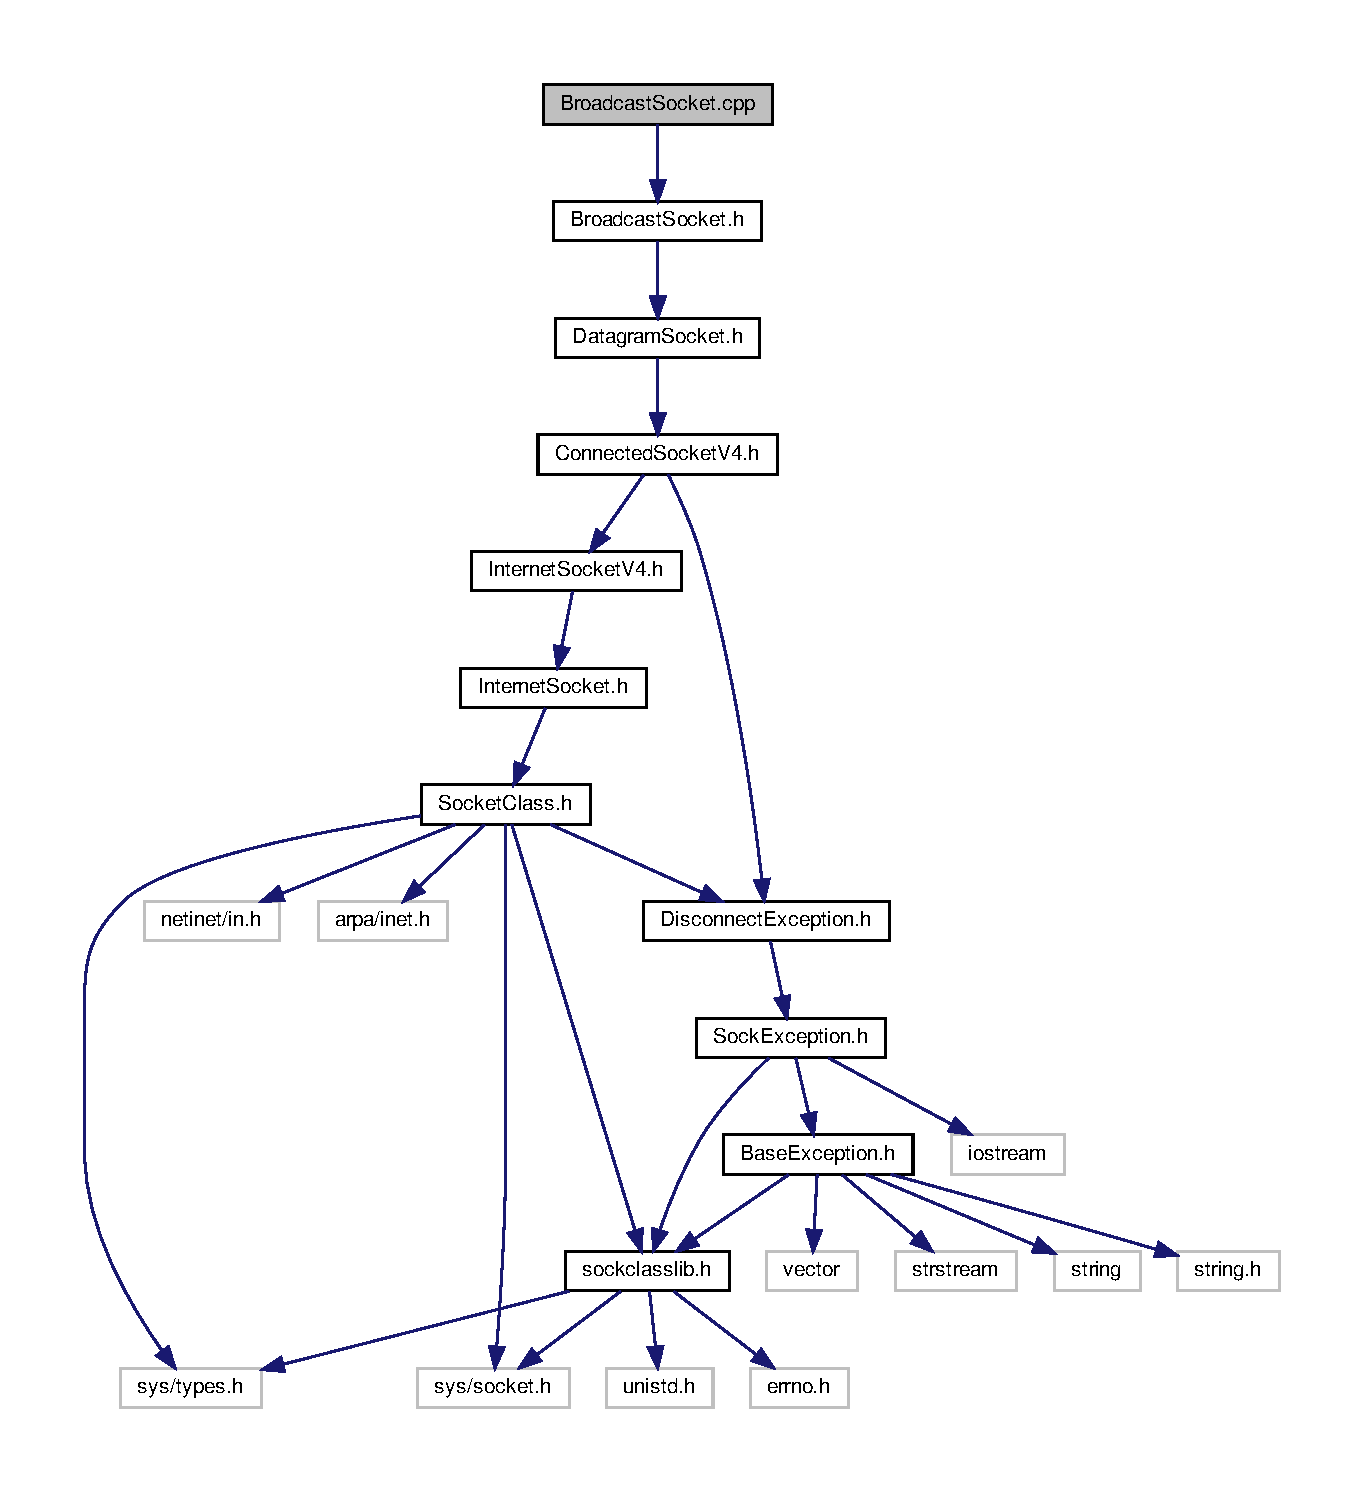
\includegraphics[width=350pt]{BroadcastSocket_8cpp__incl}
\end{center}
\end{figure}

\hypertarget{BroadcastSocket_8h}{}\section{Broadcast\+Socket.\+h File Reference}
\label{BroadcastSocket_8h}\index{Broadcast\+Socket.\+h@{Broadcast\+Socket.\+h}}
{\ttfamily \#include $<$Datagram\+Socket.\+h$>$}\newline
Include dependency graph for Broadcast\+Socket.\+h\+:\nopagebreak
\begin{figure}[H]
\begin{center}
\leavevmode
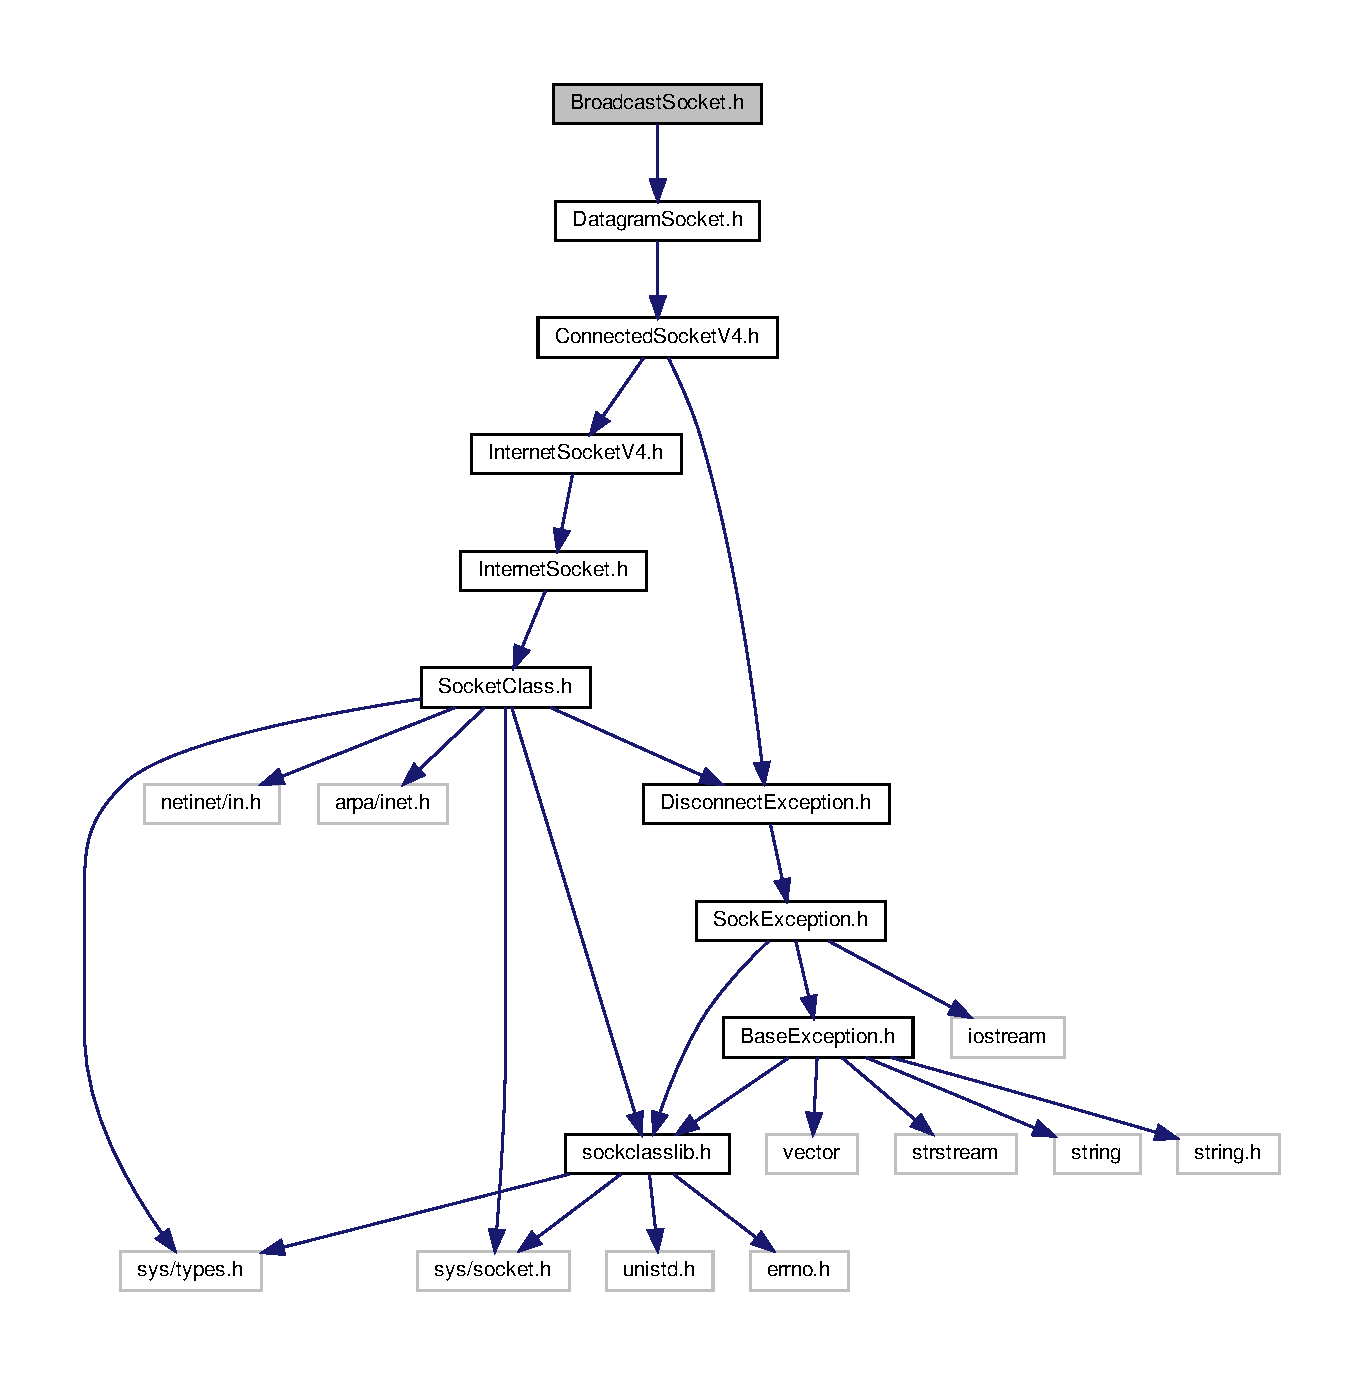
\includegraphics[width=350pt]{BroadcastSocket_8h__incl}
\end{center}
\end{figure}
This graph shows which files directly or indirectly include this file\+:\nopagebreak
\begin{figure}[H]
\begin{center}
\leavevmode
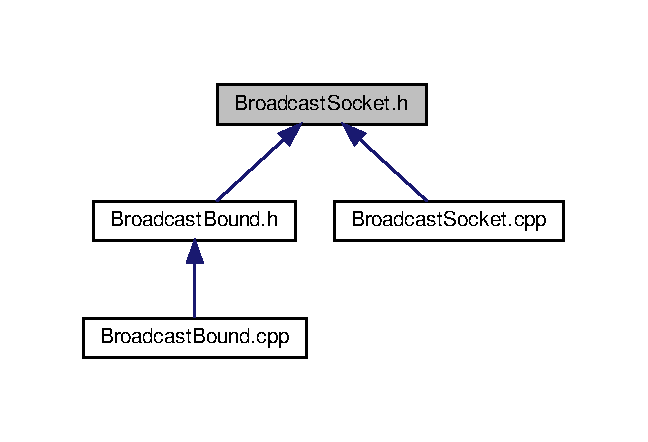
\includegraphics[width=311pt]{BroadcastSocket_8h__dep__incl}
\end{center}
\end{figure}
\subsection*{Classes}
\begin{DoxyCompactItemize}
\item 
class \hyperlink{classBroadcastSocket}{Broadcast\+Socket}
\begin{DoxyCompactList}\small\item\em Broadcast socket class. \end{DoxyCompactList}\end{DoxyCompactItemize}

\hypertarget{ClientBound_8h}{}\section{Client\+Bound.\+h File Reference}
\label{ClientBound_8h}\index{Client\+Bound.\+h@{Client\+Bound.\+h}}
{\ttfamily \#include $<$Client\+Simple.\+h$>$}\newline
{\ttfamily \#include $<$Bound\+Socket\+V4.\+h$>$}\newline
Include dependency graph for Client\+Bound.\+h\+:\nopagebreak
\begin{figure}[H]
\begin{center}
\leavevmode
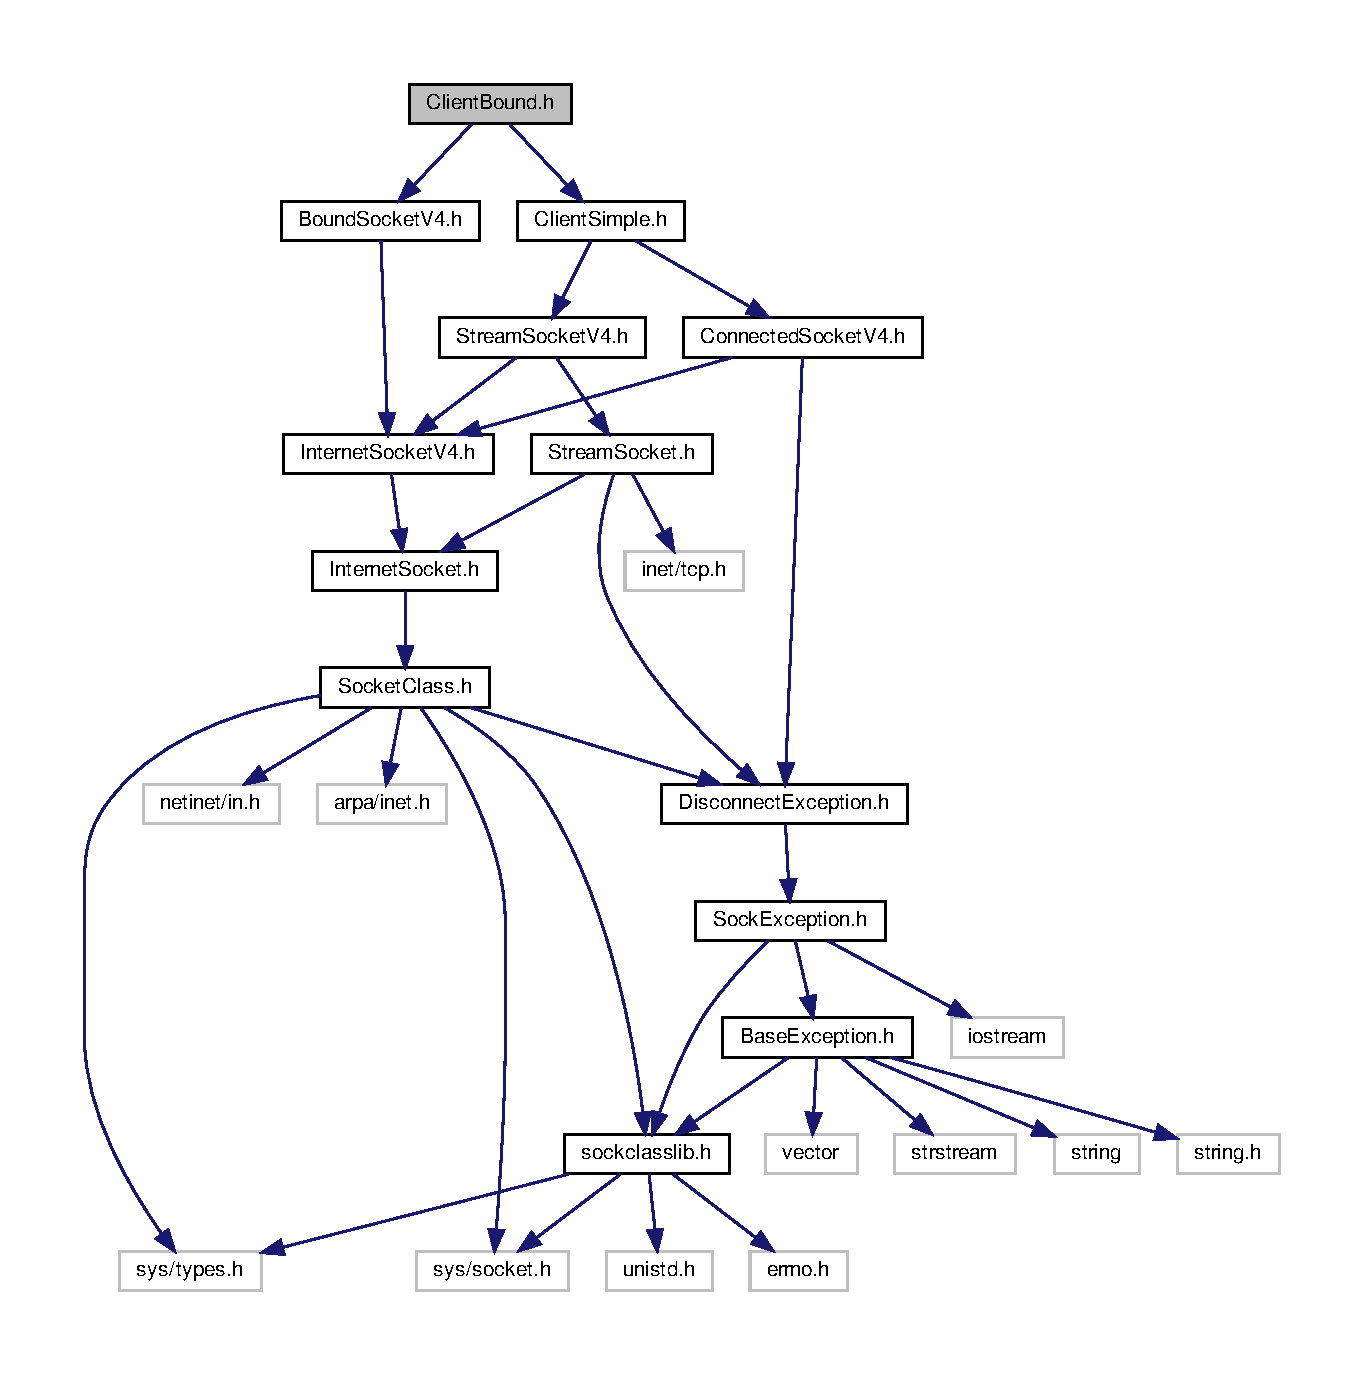
\includegraphics[width=350pt]{ClientBound_8h__incl}
\end{center}
\end{figure}
\subsection*{Classes}
\begin{DoxyCompactItemize}
\item 
class \hyperlink{classClientBound}{Client\+Bound}
\begin{DoxyCompactList}\small\item\em Client socket bound to specified port and address. \end{DoxyCompactList}\end{DoxyCompactItemize}

\hypertarget{ClientBoundV6_8h}{}\section{Client\+Bound\+V6.\+h File Reference}
\label{ClientBoundV6_8h}\index{Client\+Bound\+V6.\+h@{Client\+Bound\+V6.\+h}}
{\ttfamily \#include $<$Client\+Simple\+V6.\+h$>$}\newline
{\ttfamily \#include $<$Bound\+Socket\+V6.\+h$>$}\newline
Include dependency graph for Client\+Bound\+V6.\+h\+:\nopagebreak
\begin{figure}[H]
\begin{center}
\leavevmode
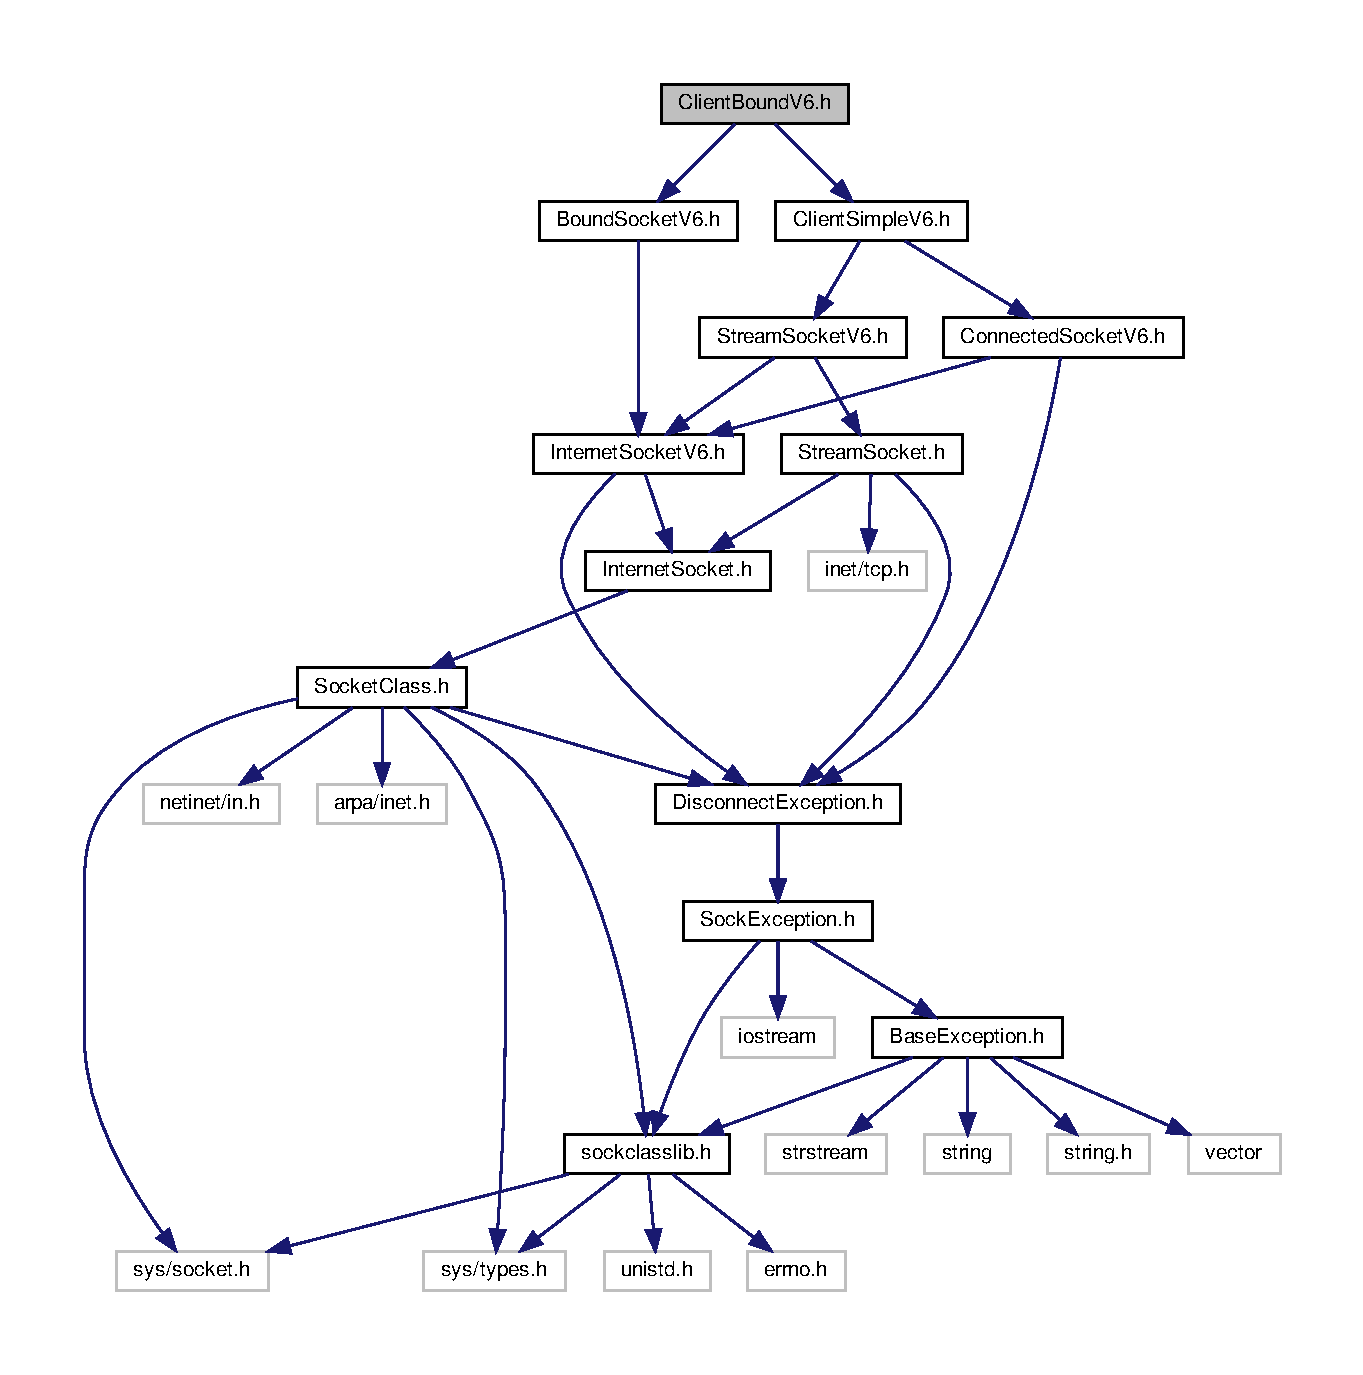
\includegraphics[width=350pt]{ClientBoundV6_8h__incl}
\end{center}
\end{figure}
\subsection*{Classes}
\begin{DoxyCompactItemize}
\item 
class \hyperlink{classClientBoundV6}{Client\+Bound\+V6}
\begin{DoxyCompactList}\small\item\em Client socket bound to specified port and address. \end{DoxyCompactList}\end{DoxyCompactItemize}

\hypertarget{ClientSimple_8h}{}\section{Client\+Simple.\+h File Reference}
\label{ClientSimple_8h}\index{Client\+Simple.\+h@{Client\+Simple.\+h}}
{\ttfamily \#include $<$Stream\+Socket\+V4.\+h$>$}\newline
{\ttfamily \#include $<$Connected\+Socket\+V4.\+h$>$}\newline
Include dependency graph for Client\+Simple.\+h\+:\nopagebreak
\begin{figure}[H]
\begin{center}
\leavevmode
\includegraphics[width=350pt]{ClientSimple_8h__incl}
\end{center}
\end{figure}
This graph shows which files directly or indirectly include this file\+:\nopagebreak
\begin{figure}[H]
\begin{center}
\leavevmode
\includegraphics[width=160pt]{ClientSimple_8h__dep__incl}
\end{center}
\end{figure}
\subsection*{Classes}
\begin{DoxyCompactItemize}
\item 
class \hyperlink{classClientSimple}{Client\+Simple}
\begin{DoxyCompactList}\small\item\em Stream oriented socket with connection ability. \end{DoxyCompactList}\end{DoxyCompactItemize}

\hypertarget{ClientSimpleV6_8h}{}\section{Client\+Simple\+V6.\+h File Reference}
\label{ClientSimpleV6_8h}\index{Client\+Simple\+V6.\+h@{Client\+Simple\+V6.\+h}}
{\ttfamily \#include $<$Stream\+Socket\+V6.\+h$>$}\newline
{\ttfamily \#include $<$Connected\+Socket\+V6.\+h$>$}\newline
Include dependency graph for Client\+Simple\+V6.\+h\+:\nopagebreak
\begin{figure}[H]
\begin{center}
\leavevmode
\includegraphics[width=350pt]{ClientSimpleV6_8h__incl}
\end{center}
\end{figure}
This graph shows which files directly or indirectly include this file\+:\nopagebreak
\begin{figure}[H]
\begin{center}
\leavevmode
\includegraphics[width=172pt]{ClientSimpleV6_8h__dep__incl}
\end{center}
\end{figure}
\subsection*{Classes}
\begin{DoxyCompactItemize}
\item 
class \hyperlink{classClientSimpleV6}{Client\+Simple\+V6}
\begin{DoxyCompactList}\small\item\em Stream oriented socket with connection ability for I\+Pv6. \end{DoxyCompactList}\end{DoxyCompactItemize}

\hypertarget{ConnectedSocketV4_8cpp}{}\section{Connected\+Socket\+V4.\+cpp File Reference}
\label{ConnectedSocketV4_8cpp}\index{Connected\+Socket\+V4.\+cpp@{Connected\+Socket\+V4.\+cpp}}
{\ttfamily \#include $<$Connected\+Socket\+V4.\+h$>$}\newline
Include dependency graph for Connected\+Socket\+V4.\+cpp\+:\nopagebreak
\begin{figure}[H]
\begin{center}
\leavevmode
\includegraphics[width=350pt]{ConnectedSocketV4_8cpp__incl}
\end{center}
\end{figure}

\hypertarget{ConnectedSocketV4_8h}{}\section{Connected\+Socket\+V4.\+h File Reference}
\label{ConnectedSocketV4_8h}\index{Connected\+Socket\+V4.\+h@{Connected\+Socket\+V4.\+h}}
{\ttfamily \#include $<$Internet\+Socket\+V4.\+h$>$}\newline
{\ttfamily \#include $<$Disconnect\+Exception.\+h$>$}\newline
Include dependency graph for Connected\+Socket\+V4.\+h\+:\nopagebreak
\begin{figure}[H]
\begin{center}
\leavevmode
\includegraphics[width=350pt]{ConnectedSocketV4_8h__incl}
\end{center}
\end{figure}
This graph shows which files directly or indirectly include this file\+:\nopagebreak
\begin{figure}[H]
\begin{center}
\leavevmode
\includegraphics[width=350pt]{ConnectedSocketV4_8h__dep__incl}
\end{center}
\end{figure}
\subsection*{Classes}
\begin{DoxyCompactItemize}
\item 
class \hyperlink{classConnectedSocketV4}{Connected\+Socket\+V4}
\begin{DoxyCompactList}\small\item\em Socket that can connect to another. \end{DoxyCompactList}\end{DoxyCompactItemize}

\hypertarget{ConnectedSocketV6_8cpp}{}\section{Connected\+Socket\+V6.\+cpp File Reference}
\label{ConnectedSocketV6_8cpp}\index{Connected\+Socket\+V6.\+cpp@{Connected\+Socket\+V6.\+cpp}}
{\ttfamily \#include \char`\"{}Connected\+Socket\+V6.\+h\char`\"{}}\newline
Include dependency graph for Connected\+Socket\+V6.\+cpp\+:\nopagebreak
\begin{figure}[H]
\begin{center}
\leavevmode
\includegraphics[width=350pt]{ConnectedSocketV6_8cpp__incl}
\end{center}
\end{figure}

\hypertarget{ConnectedSocketV6_8h}{}\section{Connected\+Socket\+V6.\+h File Reference}
\label{ConnectedSocketV6_8h}\index{Connected\+Socket\+V6.\+h@{Connected\+Socket\+V6.\+h}}
{\ttfamily \#include $<$Internet\+Socket\+V6.\+h$>$}\newline
{\ttfamily \#include $<$Disconnect\+Exception.\+h$>$}\newline
Include dependency graph for Connected\+Socket\+V6.\+h\+:\nopagebreak
\begin{figure}[H]
\begin{center}
\leavevmode
\includegraphics[width=350pt]{ConnectedSocketV6_8h__incl}
\end{center}
\end{figure}
This graph shows which files directly or indirectly include this file\+:\nopagebreak
\begin{figure}[H]
\begin{center}
\leavevmode
\includegraphics[width=350pt]{ConnectedSocketV6_8h__dep__incl}
\end{center}
\end{figure}
\subsection*{Classes}
\begin{DoxyCompactItemize}
\item 
class \hyperlink{classConnectedSocketV6}{Connected\+Socket\+V6}
\begin{DoxyCompactList}\small\item\em Socket that can connect to another. \end{DoxyCompactList}\end{DoxyCompactItemize}

\hypertarget{DatagramBound_8cpp}{}\section{Datagram\+Bound.\+cpp File Reference}
\label{DatagramBound_8cpp}\index{Datagram\+Bound.\+cpp@{Datagram\+Bound.\+cpp}}
{\ttfamily \#include $<$Datagram\+Bound.\+h$>$}\newline
Include dependency graph for Datagram\+Bound.\+cpp\+:\nopagebreak
\begin{figure}[H]
\begin{center}
\leavevmode
\includegraphics[width=350pt]{DatagramBound_8cpp__incl}
\end{center}
\end{figure}

\hypertarget{DatagramBound_8h}{}\section{Datagram\+Bound.\+h File Reference}
\label{DatagramBound_8h}\index{Datagram\+Bound.\+h@{Datagram\+Bound.\+h}}
{\ttfamily \#include $<$Datagram\+Socket.\+h$>$}\newline
{\ttfamily \#include $<$Bound\+Socket\+V4.\+h$>$}\newline
Include dependency graph for Datagram\+Bound.\+h\+:\nopagebreak
\begin{figure}[H]
\begin{center}
\leavevmode
\includegraphics[width=350pt]{DatagramBound_8h__incl}
\end{center}
\end{figure}
This graph shows which files directly or indirectly include this file\+:\nopagebreak
\begin{figure}[H]
\begin{center}
\leavevmode
\includegraphics[width=186pt]{DatagramBound_8h__dep__incl}
\end{center}
\end{figure}
\subsection*{Classes}
\begin{DoxyCompactItemize}
\item 
class \hyperlink{classDatagramBound}{Datagram\+Bound}
\begin{DoxyCompactList}\small\item\em U\+DP socket bound to specified port and address (aka U\+DP server). \end{DoxyCompactList}\end{DoxyCompactItemize}

\hypertarget{DatagramBoundV6_8cpp}{}\section{Datagram\+Bound\+V6.\+cpp File Reference}
\label{DatagramBoundV6_8cpp}\index{Datagram\+Bound\+V6.\+cpp@{Datagram\+Bound\+V6.\+cpp}}
{\ttfamily \#include $<$Datagram\+Bound\+V6.\+h$>$}\newline
Include dependency graph for Datagram\+Bound\+V6.\+cpp\+:\nopagebreak
\begin{figure}[H]
\begin{center}
\leavevmode
\includegraphics[width=350pt]{DatagramBoundV6_8cpp__incl}
\end{center}
\end{figure}

\hypertarget{DatagramBoundV6_8h}{}\section{Datagram\+Bound\+V6.\+h File Reference}
\label{DatagramBoundV6_8h}\index{Datagram\+Bound\+V6.\+h@{Datagram\+Bound\+V6.\+h}}
{\ttfamily \#include $<$Datagram\+Socket\+V6.\+h$>$}\newline
{\ttfamily \#include $<$Bound\+Socket\+V6.\+h$>$}\newline
Include dependency graph for Datagram\+Bound\+V6.\+h\+:\nopagebreak
\begin{figure}[H]
\begin{center}
\leavevmode
\includegraphics[width=350pt]{DatagramBoundV6_8h__incl}
\end{center}
\end{figure}
This graph shows which files directly or indirectly include this file\+:\nopagebreak
\begin{figure}[H]
\begin{center}
\leavevmode
\includegraphics[width=198pt]{DatagramBoundV6_8h__dep__incl}
\end{center}
\end{figure}
\subsection*{Classes}
\begin{DoxyCompactItemize}
\item 
class \hyperlink{classDatagramBoundV6}{Datagram\+Bound\+V6}
\begin{DoxyCompactList}\small\item\em U\+DP socket bound to specified port and address (aka U\+DP server) for I\+Pv6. \end{DoxyCompactList}\end{DoxyCompactItemize}

\hypertarget{DatagramSocket_8cpp}{}\section{Datagram\+Socket.\+cpp File Reference}
\label{DatagramSocket_8cpp}\index{Datagram\+Socket.\+cpp@{Datagram\+Socket.\+cpp}}
{\ttfamily \#include $<$Datagram\+Socket.\+h$>$}\newline
{\ttfamily \#include $<$string.\+h$>$}\newline
Include dependency graph for Datagram\+Socket.\+cpp\+:\nopagebreak
\begin{figure}[H]
\begin{center}
\leavevmode
\includegraphics[width=350pt]{DatagramSocket_8cpp__incl}
\end{center}
\end{figure}
\subsection*{Macros}
\begin{DoxyCompactItemize}
\item 
\#define \hyperlink{DatagramSocket_8cpp_a403340f0d24de144ba88d722b84cb4c9}{S\+I\+O\+\_\+\+U\+D\+P\+\_\+\+C\+O\+N\+N\+R\+E\+S\+ET}~\+\_\+\+W\+S\+A\+I\+OW(I\+O\+C\+\_\+\+V\+E\+N\+D\+OR,12)
\end{DoxyCompactItemize}


\subsection{Macro Definition Documentation}
\mbox{\Hypertarget{DatagramSocket_8cpp_a403340f0d24de144ba88d722b84cb4c9}\label{DatagramSocket_8cpp_a403340f0d24de144ba88d722b84cb4c9}} 
\index{Datagram\+Socket.\+cpp@{Datagram\+Socket.\+cpp}!S\+I\+O\+\_\+\+U\+D\+P\+\_\+\+C\+O\+N\+N\+R\+E\+S\+ET@{S\+I\+O\+\_\+\+U\+D\+P\+\_\+\+C\+O\+N\+N\+R\+E\+S\+ET}}
\index{S\+I\+O\+\_\+\+U\+D\+P\+\_\+\+C\+O\+N\+N\+R\+E\+S\+ET@{S\+I\+O\+\_\+\+U\+D\+P\+\_\+\+C\+O\+N\+N\+R\+E\+S\+ET}!Datagram\+Socket.\+cpp@{Datagram\+Socket.\+cpp}}
\subsubsection{\texorpdfstring{S\+I\+O\+\_\+\+U\+D\+P\+\_\+\+C\+O\+N\+N\+R\+E\+S\+ET}{SIO\_UDP\_CONNRESET}}
{\footnotesize\ttfamily \#define S\+I\+O\+\_\+\+U\+D\+P\+\_\+\+C\+O\+N\+N\+R\+E\+S\+ET~\+\_\+\+W\+S\+A\+I\+OW(I\+O\+C\+\_\+\+V\+E\+N\+D\+OR,12)}


\hypertarget{DatagramSocket_8h}{}\section{Datagram\+Socket.\+h File Reference}
\label{DatagramSocket_8h}\index{Datagram\+Socket.\+h@{Datagram\+Socket.\+h}}
{\ttfamily \#include $<$Connected\+Socket\+V4.\+h$>$}\newline
Include dependency graph for Datagram\+Socket.\+h\+:\nopagebreak
\begin{figure}[H]
\begin{center}
\leavevmode
\includegraphics[width=350pt]{DatagramSocket_8h__incl}
\end{center}
\end{figure}
This graph shows which files directly or indirectly include this file\+:\nopagebreak
\begin{figure}[H]
\begin{center}
\leavevmode
\includegraphics[width=350pt]{DatagramSocket_8h__dep__incl}
\end{center}
\end{figure}
\subsection*{Classes}
\begin{DoxyCompactItemize}
\item 
class \hyperlink{classDatagramSocket}{Datagram\+Socket}
\begin{DoxyCompactList}\small\item\em Class for U\+DP sockets. \end{DoxyCompactList}\end{DoxyCompactItemize}

\hypertarget{DatagramSocketV6_8cpp}{}\section{Datagram\+Socket\+V6.\+cpp File Reference}
\label{DatagramSocketV6_8cpp}\index{Datagram\+Socket\+V6.\+cpp@{Datagram\+Socket\+V6.\+cpp}}
{\ttfamily \#include $<$Datagram\+Socket\+V6.\+h$>$}\newline
{\ttfamily \#include $<$string.\+h$>$}\newline
Include dependency graph for Datagram\+Socket\+V6.\+cpp\+:\nopagebreak
\begin{figure}[H]
\begin{center}
\leavevmode
\includegraphics[width=350pt]{DatagramSocketV6_8cpp__incl}
\end{center}
\end{figure}
\subsection*{Macros}
\begin{DoxyCompactItemize}
\item 
\#define \hyperlink{DatagramSocketV6_8cpp_a403340f0d24de144ba88d722b84cb4c9}{S\+I\+O\+\_\+\+U\+D\+P\+\_\+\+C\+O\+N\+N\+R\+E\+S\+ET}~\+\_\+\+W\+S\+A\+I\+OW(I\+O\+C\+\_\+\+V\+E\+N\+D\+OR,12)
\end{DoxyCompactItemize}


\subsection{Macro Definition Documentation}
\mbox{\Hypertarget{DatagramSocketV6_8cpp_a403340f0d24de144ba88d722b84cb4c9}\label{DatagramSocketV6_8cpp_a403340f0d24de144ba88d722b84cb4c9}} 
\index{Datagram\+Socket\+V6.\+cpp@{Datagram\+Socket\+V6.\+cpp}!S\+I\+O\+\_\+\+U\+D\+P\+\_\+\+C\+O\+N\+N\+R\+E\+S\+ET@{S\+I\+O\+\_\+\+U\+D\+P\+\_\+\+C\+O\+N\+N\+R\+E\+S\+ET}}
\index{S\+I\+O\+\_\+\+U\+D\+P\+\_\+\+C\+O\+N\+N\+R\+E\+S\+ET@{S\+I\+O\+\_\+\+U\+D\+P\+\_\+\+C\+O\+N\+N\+R\+E\+S\+ET}!Datagram\+Socket\+V6.\+cpp@{Datagram\+Socket\+V6.\+cpp}}
\subsubsection{\texorpdfstring{S\+I\+O\+\_\+\+U\+D\+P\+\_\+\+C\+O\+N\+N\+R\+E\+S\+ET}{SIO\_UDP\_CONNRESET}}
{\footnotesize\ttfamily \#define S\+I\+O\+\_\+\+U\+D\+P\+\_\+\+C\+O\+N\+N\+R\+E\+S\+ET~\+\_\+\+W\+S\+A\+I\+OW(I\+O\+C\+\_\+\+V\+E\+N\+D\+OR,12)}


\hypertarget{DatagramSocketV6_8h}{}\section{Datagram\+Socket\+V6.\+h File Reference}
\label{DatagramSocketV6_8h}\index{Datagram\+Socket\+V6.\+h@{Datagram\+Socket\+V6.\+h}}
{\ttfamily \#include $<$Connected\+Socket\+V6.\+h$>$}\newline
Include dependency graph for Datagram\+Socket\+V6.\+h\+:\nopagebreak
\begin{figure}[H]
\begin{center}
\leavevmode
\includegraphics[width=350pt]{DatagramSocketV6_8h__incl}
\end{center}
\end{figure}
This graph shows which files directly or indirectly include this file\+:\nopagebreak
\begin{figure}[H]
\begin{center}
\leavevmode
\includegraphics[width=350pt]{DatagramSocketV6_8h__dep__incl}
\end{center}
\end{figure}
\subsection*{Classes}
\begin{DoxyCompactItemize}
\item 
class \hyperlink{classDatagramSocketV6}{Datagram\+Socket\+V6}
\begin{DoxyCompactList}\small\item\em Class for U\+DP sockets I\+Pv6. \end{DoxyCompactList}\end{DoxyCompactItemize}

\hypertarget{DisconnectException_8h}{}\section{Disconnect\+Exception.\+h File Reference}
\label{DisconnectException_8h}\index{Disconnect\+Exception.\+h@{Disconnect\+Exception.\+h}}
{\ttfamily \#include $<$Sock\+Exception.\+h$>$}\newline
Include dependency graph for Disconnect\+Exception.\+h\+:\nopagebreak
\begin{figure}[H]
\begin{center}
\leavevmode
\includegraphics[width=350pt]{DisconnectException_8h__incl}
\end{center}
\end{figure}
This graph shows which files directly or indirectly include this file\+:\nopagebreak
\begin{figure}[H]
\begin{center}
\leavevmode
\includegraphics[width=350pt]{DisconnectException_8h__dep__incl}
\end{center}
\end{figure}
\subsection*{Classes}
\begin{DoxyCompactItemize}
\item 
class \hyperlink{classDisconnectException}{Disconnect\+Exception}
\end{DoxyCompactItemize}
\subsection*{Macros}
\begin{DoxyCompactItemize}
\item 
\#define \hyperlink{group__EXCEPT__GROUP_ga9271529edaf4938342fe2c16ea4539a2}{D\+I\+S\+C\+O\+N\+N\+\_\+\+E\+X\+C\+E\+P\+T\+\_\+\+T\+H\+R\+OW}(x)
\begin{DoxyCompactList}\small\item\em Throw disconnect exception. \end{DoxyCompactList}\item 
\#define \hyperlink{group__EXCEPT__GROUP_gaf912806beff3d8ce88b3a42ad6b40550}{D\+I\+S\+C\+O\+N\+N\+\_\+\+E\+X\+C\+E\+P\+T\+\_\+\+C\+A\+T\+C\+H\+\_\+\+A\+N\+D\+\_\+\+R\+A\+I\+SE}(x)
\begin{DoxyCompactList}\small\item\em Catch and re-\/throw disconnect exception. \end{DoxyCompactList}\item 
\#define \hyperlink{group__EXCEPT__GROUP_ga20a7d853d1b1747473acd142d59243d2}{D\+I\+S\+C\+O\+N\+N\+\_\+\+E\+X\+C\+E\+P\+T\+\_\+\+C\+A\+T\+C\+H\+\_\+\+B\+E\+G\+IN}(x)
\begin{DoxyCompactList}\small\item\em Catch disconnect exception with report. Opens catch block. \end{DoxyCompactList}\item 
\#define \hyperlink{group__EXCEPT__GROUP_ga1319e3cfc7ea4e32ae6ec2b2932df669}{D\+I\+S\+C\+O\+N\+N\+\_\+\+E\+X\+C\+E\+P\+T\+\_\+\+C\+A\+T\+C\+H\+\_\+\+B\+E\+G\+I\+N\+\_\+\+N\+O\+R\+EP}
\begin{DoxyCompactList}\small\item\em Catch disconnect exception without report. Opens catch block. \end{DoxyCompactList}\item 
\#define \hyperlink{group__EXCEPT__GROUP_ga68eddf699cb35b0ba76d737545b24167}{D\+I\+S\+C\+O\+N\+N\+\_\+\+E\+X\+C\+E\+P\+T\+\_\+\+C\+A\+T\+C\+H\+\_\+\+A\+LL}(x)
\begin{DoxyCompactList}\small\item\em Catch all aka catch(...) \end{DoxyCompactList}\item 
\#define \hyperlink{group__EXCEPT__GROUP_ga142715775c6f4ff27e2a88a424a3bbb4}{D\+I\+S\+C\+O\+N\+N\+\_\+\+E\+X\+C\+E\+P\+T\+\_\+\+C\+A\+T\+C\+H\+\_\+\+E\+ND}~\}
\begin{DoxyCompactList}\small\item\em Close catch block. \end{DoxyCompactList}\item 
\#define \hyperlink{group__EXCEPT__GROUP_gac13aeebcd10acdb772f18e65e1c688c1}{D\+I\+S\+C\+O\+N\+N\+\_\+\+T\+RY}~try
\begin{DoxyCompactList}\small\item\em Try. \end{DoxyCompactList}\end{DoxyCompactItemize}

\hypertarget{InternetSocket_8h}{}\section{Internet\+Socket.\+h File Reference}
\label{InternetSocket_8h}\index{Internet\+Socket.\+h@{Internet\+Socket.\+h}}
{\ttfamily \#include $<$Socket\+Class.\+h$>$}\newline
Include dependency graph for Internet\+Socket.\+h\+:\nopagebreak
\begin{figure}[H]
\begin{center}
\leavevmode
\includegraphics[width=350pt]{InternetSocket_8h__incl}
\end{center}
\end{figure}
This graph shows which files directly or indirectly include this file\+:\nopagebreak
\begin{figure}[H]
\begin{center}
\leavevmode
\includegraphics[width=350pt]{InternetSocket_8h__dep__incl}
\end{center}
\end{figure}
\subsection*{Classes}
\begin{DoxyCompactItemize}
\item 
class \hyperlink{classInternetSocket}{Internet\+Socket}
\end{DoxyCompactItemize}

\hypertarget{InternetSocketV4_8cpp}{}\section{Internet\+Socket\+V4.\+cpp File Reference}
\label{InternetSocketV4_8cpp}\index{Internet\+Socket\+V4.\+cpp@{Internet\+Socket\+V4.\+cpp}}
{\ttfamily \#include $<$Internet\+Socket\+V4.\+h$>$}\newline
Include dependency graph for Internet\+Socket\+V4.\+cpp\+:\nopagebreak
\begin{figure}[H]
\begin{center}
\leavevmode
\includegraphics[width=350pt]{InternetSocketV4_8cpp__incl}
\end{center}
\end{figure}

\hypertarget{InternetSocketV4_8h}{}\section{Internet\+Socket\+V4.\+h File Reference}
\label{InternetSocketV4_8h}\index{Internet\+Socket\+V4.\+h@{Internet\+Socket\+V4.\+h}}
{\ttfamily \#include $<$Internet\+Socket.\+h$>$}\newline
Include dependency graph for Internet\+Socket\+V4.\+h\+:\nopagebreak
\begin{figure}[H]
\begin{center}
\leavevmode
\includegraphics[width=350pt]{InternetSocketV4_8h__incl}
\end{center}
\end{figure}
This graph shows which files directly or indirectly include this file\+:\nopagebreak
\begin{figure}[H]
\begin{center}
\leavevmode
\includegraphics[width=350pt]{InternetSocketV4_8h__dep__incl}
\end{center}
\end{figure}
\subsection*{Classes}
\begin{DoxyCompactItemize}
\item 
class \hyperlink{classInternetSocketV4}{Internet\+Socket\+V4}
\end{DoxyCompactItemize}

\hypertarget{InternetSocketV6_8cpp}{}\section{Internet\+Socket\+V6.\+cpp File Reference}
\label{InternetSocketV6_8cpp}\index{Internet\+Socket\+V6.\+cpp@{Internet\+Socket\+V6.\+cpp}}
{\ttfamily \#include $<$Internet\+Socket\+V6.\+h$>$}\newline
Include dependency graph for Internet\+Socket\+V6.\+cpp\+:\nopagebreak
\begin{figure}[H]
\begin{center}
\leavevmode
\includegraphics[width=350pt]{InternetSocketV6_8cpp__incl}
\end{center}
\end{figure}

\hypertarget{InternetSocketV6_8h}{}\section{Internet\+Socket\+V6.\+h File Reference}
\label{InternetSocketV6_8h}\index{Internet\+Socket\+V6.\+h@{Internet\+Socket\+V6.\+h}}
{\ttfamily \#include $<$Internet\+Socket.\+h$>$}\newline
{\ttfamily \#include $<$Disconnect\+Exception.\+h$>$}\newline
Include dependency graph for Internet\+Socket\+V6.\+h\+:\nopagebreak
\begin{figure}[H]
\begin{center}
\leavevmode
\includegraphics[width=350pt]{InternetSocketV6_8h__incl}
\end{center}
\end{figure}
This graph shows which files directly or indirectly include this file\+:\nopagebreak
\begin{figure}[H]
\begin{center}
\leavevmode
\includegraphics[width=350pt]{InternetSocketV6_8h__dep__incl}
\end{center}
\end{figure}
\subsection*{Classes}
\begin{DoxyCompactItemize}
\item 
class \hyperlink{classInternetSocketV6}{Internet\+Socket\+V6}
\end{DoxyCompactItemize}

\hypertarget{MulticastBound_8cpp}{}\section{Multicast\+Bound.\+cpp File Reference}
\label{MulticastBound_8cpp}\index{Multicast\+Bound.\+cpp@{Multicast\+Bound.\+cpp}}
{\ttfamily \#include $<$Multicast\+Bound.\+h$>$}\newline
{\ttfamily \#include $<$errno.\+h$>$}\newline
{\ttfamily \#include $<$algorithm$>$}\newline
Include dependency graph for Multicast\+Bound.\+cpp\+:\nopagebreak
\begin{figure}[H]
\begin{center}
\leavevmode
\includegraphics[width=350pt]{MulticastBound_8cpp__incl}
\end{center}
\end{figure}

\hypertarget{MulticastBound_8h}{}\section{Multicast\+Bound.\+h File Reference}
\label{MulticastBound_8h}\index{Multicast\+Bound.\+h@{Multicast\+Bound.\+h}}
{\ttfamily \#include $<$Multicast\+Socket.\+h$>$}\newline
{\ttfamily \#include $<$Bound\+Socket\+V4.\+h$>$}\newline
{\ttfamily \#include $<$list$>$}\newline
Include dependency graph for Multicast\+Bound.\+h\+:\nopagebreak
\begin{figure}[H]
\begin{center}
\leavevmode
\includegraphics[width=350pt]{MulticastBound_8h__incl}
\end{center}
\end{figure}
This graph shows which files directly or indirectly include this file\+:\nopagebreak
\begin{figure}[H]
\begin{center}
\leavevmode
\includegraphics[width=183pt]{MulticastBound_8h__dep__incl}
\end{center}
\end{figure}
\subsection*{Classes}
\begin{DoxyCompactItemize}
\item 
class \hyperlink{classMulticastBound}{Multicast\+Bound}
\begin{DoxyCompactList}\small\item\em I\+Pv4 socket capable to receive multicast datagrams. \end{DoxyCompactList}\end{DoxyCompactItemize}
\subsection*{Typedefs}
\begin{DoxyCompactItemize}
\item 
typedef list$<$ in\+\_\+addr\+\_\+t $>$ \hyperlink{MulticastBound_8h_a9584173a620a338ea7d88264229e36dd}{Groups\+List\+Type}
\end{DoxyCompactItemize}


\subsection{Typedef Documentation}
\mbox{\Hypertarget{MulticastBound_8h_a9584173a620a338ea7d88264229e36dd}\label{MulticastBound_8h_a9584173a620a338ea7d88264229e36dd}} 
\index{Multicast\+Bound.\+h@{Multicast\+Bound.\+h}!Groups\+List\+Type@{Groups\+List\+Type}}
\index{Groups\+List\+Type@{Groups\+List\+Type}!Multicast\+Bound.\+h@{Multicast\+Bound.\+h}}
\subsubsection{\texorpdfstring{Groups\+List\+Type}{GroupsListType}}
{\footnotesize\ttfamily typedef list$<$ in\+\_\+addr\+\_\+t $>$ \hyperlink{MulticastBound_8h_a9584173a620a338ea7d88264229e36dd}{Groups\+List\+Type}}


\hypertarget{MulticastBoundV6_8cpp}{}\section{Multicast\+Bound\+V6.\+cpp File Reference}
\label{MulticastBoundV6_8cpp}\index{Multicast\+Bound\+V6.\+cpp@{Multicast\+Bound\+V6.\+cpp}}
{\ttfamily \#include \char`\"{}Multicast\+Bound\+V6.\+h\char`\"{}}\newline
{\ttfamily \#include $<$errno.\+h$>$}\newline
{\ttfamily \#include $<$algorithm$>$}\newline
Include dependency graph for Multicast\+Bound\+V6.\+cpp\+:\nopagebreak
\begin{figure}[H]
\begin{center}
\leavevmode
\includegraphics[width=350pt]{MulticastBoundV6_8cpp__incl}
\end{center}
\end{figure}

\hypertarget{MulticastBoundV6_8h}{}\section{Multicast\+Bound\+V6.\+h File Reference}
\label{MulticastBoundV6_8h}\index{Multicast\+Bound\+V6.\+h@{Multicast\+Bound\+V6.\+h}}
{\ttfamily \#include $<$Multicast\+Socket\+V6.\+h$>$}\newline
{\ttfamily \#include $<$Bound\+Socket\+V6.\+h$>$}\newline
{\ttfamily \#include $<$list$>$}\newline
Include dependency graph for Multicast\+Bound\+V6.\+h\+:\nopagebreak
\begin{figure}[H]
\begin{center}
\leavevmode
\includegraphics[width=350pt]{MulticastBoundV6_8h__incl}
\end{center}
\end{figure}
This graph shows which files directly or indirectly include this file\+:\nopagebreak
\begin{figure}[H]
\begin{center}
\leavevmode
\includegraphics[width=195pt]{MulticastBoundV6_8h__dep__incl}
\end{center}
\end{figure}
\subsection*{Classes}
\begin{DoxyCompactItemize}
\item 
class \hyperlink{classMulticastBoundV6}{Multicast\+Bound\+V6}
\begin{DoxyCompactList}\small\item\em I\+Pv4 socket capable to receive multicast datagrams. \end{DoxyCompactList}\end{DoxyCompactItemize}
\subsection*{Typedefs}
\begin{DoxyCompactItemize}
\item 
typedef list$<$ in6\+\_\+addr $>$ \hyperlink{MulticastBoundV6_8h_af9609f9ebdd5cf62a0d27943c53d74a2}{Groups\+List\+Type}
\end{DoxyCompactItemize}
\subsection*{Functions}
\begin{DoxyCompactItemize}
\item 
bool \hyperlink{MulticastBoundV6_8h_adbff503e083ab6fdb1b15fe9c1a81496}{operator==} (const in6\+\_\+addr \&left, const in6\+\_\+addr \&right)
\end{DoxyCompactItemize}


\subsection{Typedef Documentation}
\mbox{\Hypertarget{MulticastBoundV6_8h_af9609f9ebdd5cf62a0d27943c53d74a2}\label{MulticastBoundV6_8h_af9609f9ebdd5cf62a0d27943c53d74a2}} 
\index{Multicast\+Bound\+V6.\+h@{Multicast\+Bound\+V6.\+h}!Groups\+List\+Type@{Groups\+List\+Type}}
\index{Groups\+List\+Type@{Groups\+List\+Type}!Multicast\+Bound\+V6.\+h@{Multicast\+Bound\+V6.\+h}}
\subsubsection{\texorpdfstring{Groups\+List\+Type}{GroupsListType}}
{\footnotesize\ttfamily typedef list$<$ in6\+\_\+addr $>$ \hyperlink{MulticastBound_8h_a9584173a620a338ea7d88264229e36dd}{Groups\+List\+Type}}



\subsection{Function Documentation}
\mbox{\Hypertarget{MulticastBoundV6_8h_adbff503e083ab6fdb1b15fe9c1a81496}\label{MulticastBoundV6_8h_adbff503e083ab6fdb1b15fe9c1a81496}} 
\index{Multicast\+Bound\+V6.\+h@{Multicast\+Bound\+V6.\+h}!operator==@{operator==}}
\index{operator==@{operator==}!Multicast\+Bound\+V6.\+h@{Multicast\+Bound\+V6.\+h}}
\subsubsection{\texorpdfstring{operator==()}{operator==()}}
{\footnotesize\ttfamily bool operator== (\begin{DoxyParamCaption}\item[{const in6\+\_\+addr \&}]{left,  }\item[{const in6\+\_\+addr \&}]{right }\end{DoxyParamCaption})}


\hypertarget{MulticastSocket_8cpp}{}\section{Multicast\+Socket.\+cpp File Reference}
\label{MulticastSocket_8cpp}\index{Multicast\+Socket.\+cpp@{Multicast\+Socket.\+cpp}}
{\ttfamily \#include $<$Multicast\+Socket.\+h$>$}\newline
Include dependency graph for Multicast\+Socket.\+cpp\+:\nopagebreak
\begin{figure}[H]
\begin{center}
\leavevmode
\includegraphics[width=350pt]{MulticastSocket_8cpp__incl}
\end{center}
\end{figure}

\hypertarget{MulticastSocket_8h}{}\section{Multicast\+Socket.\+h File Reference}
\label{MulticastSocket_8h}\index{Multicast\+Socket.\+h@{Multicast\+Socket.\+h}}
{\ttfamily \#include $<$Datagram\+Socket.\+h$>$}\newline
Include dependency graph for Multicast\+Socket.\+h\+:\nopagebreak
\begin{figure}[H]
\begin{center}
\leavevmode
\includegraphics[width=350pt]{MulticastSocket_8h__incl}
\end{center}
\end{figure}
This graph shows which files directly or indirectly include this file\+:\nopagebreak
\begin{figure}[H]
\begin{center}
\leavevmode
\includegraphics[width=302pt]{MulticastSocket_8h__dep__incl}
\end{center}
\end{figure}
\subsection*{Classes}
\begin{DoxyCompactItemize}
\item 
class \hyperlink{classMulticastSocket}{Multicast\+Socket}
\begin{DoxyCompactList}\small\item\em I\+Pv4 datagram socket capable to send multicast datagrams. \end{DoxyCompactList}\end{DoxyCompactItemize}

\hypertarget{MulticastSocketV6_8cpp}{}\section{Multicast\+Socket\+V6.\+cpp File Reference}
\label{MulticastSocketV6_8cpp}\index{Multicast\+Socket\+V6.\+cpp@{Multicast\+Socket\+V6.\+cpp}}
{\ttfamily \#include \char`\"{}Multicast\+Socket\+V6.\+h\char`\"{}}\newline
Include dependency graph for Multicast\+Socket\+V6.\+cpp\+:\nopagebreak
\begin{figure}[H]
\begin{center}
\leavevmode
\includegraphics[width=350pt]{MulticastSocketV6_8cpp__incl}
\end{center}
\end{figure}

\hypertarget{MulticastSocketV6_8h}{}\section{Multicast\+Socket\+V6.\+h File Reference}
\label{MulticastSocketV6_8h}\index{Multicast\+Socket\+V6.\+h@{Multicast\+Socket\+V6.\+h}}
{\ttfamily \#include $<$Datagram\+Socket\+V6.\+h$>$}\newline
Include dependency graph for Multicast\+Socket\+V6.\+h\+:\nopagebreak
\begin{figure}[H]
\begin{center}
\leavevmode
\includegraphics[width=350pt]{MulticastSocketV6_8h__incl}
\end{center}
\end{figure}
This graph shows which files directly or indirectly include this file\+:\nopagebreak
\begin{figure}[H]
\begin{center}
\leavevmode
\includegraphics[width=326pt]{MulticastSocketV6_8h__dep__incl}
\end{center}
\end{figure}
\subsection*{Classes}
\begin{DoxyCompactItemize}
\item 
class \hyperlink{classMulticastSocketV6}{Multicast\+Socket\+V6}
\begin{DoxyCompactList}\small\item\em I\+Pv6 datagram socket capable to send multicast datagrams. \end{DoxyCompactList}\end{DoxyCompactItemize}

\hypertarget{ServerReuse_8cpp}{}\section{Server\+Reuse.\+cpp File Reference}
\label{ServerReuse_8cpp}\index{Server\+Reuse.\+cpp@{Server\+Reuse.\+cpp}}
{\ttfamily \#include $<$Server\+Reuse.\+h$>$}\newline
Include dependency graph for Server\+Reuse.\+cpp\+:\nopagebreak
\begin{figure}[H]
\begin{center}
\leavevmode
\includegraphics[width=350pt]{ServerReuse_8cpp__incl}
\end{center}
\end{figure}

\hypertarget{ServerReuse_8h}{}\section{Server\+Reuse.\+h File Reference}
\label{ServerReuse_8h}\index{Server\+Reuse.\+h@{Server\+Reuse.\+h}}
{\ttfamily \#include $<$Server\+Simple.\+h$>$}\newline
Include dependency graph for Server\+Reuse.\+h\+:\nopagebreak
\begin{figure}[H]
\begin{center}
\leavevmode
\includegraphics[width=350pt]{ServerReuse_8h__incl}
\end{center}
\end{figure}
This graph shows which files directly or indirectly include this file\+:\nopagebreak
\begin{figure}[H]
\begin{center}
\leavevmode
\includegraphics[width=172pt]{ServerReuse_8h__dep__incl}
\end{center}
\end{figure}
\subsection*{Classes}
\begin{DoxyCompactItemize}
\item 
class \hyperlink{classServerReuse}{Server\+Reuse}
\begin{DoxyCompactList}\small\item\em T\+CP server socket with reuse local address ability. \end{DoxyCompactList}\end{DoxyCompactItemize}

\hypertarget{ServerReuseV6_8cpp}{}\section{Server\+Reuse\+V6.\+cpp File Reference}
\label{ServerReuseV6_8cpp}\index{Server\+Reuse\+V6.\+cpp@{Server\+Reuse\+V6.\+cpp}}
{\ttfamily \#include $<$Server\+Reuse\+V6.\+h$>$}\newline
Include dependency graph for Server\+Reuse\+V6.\+cpp\+:\nopagebreak
\begin{figure}[H]
\begin{center}
\leavevmode
\includegraphics[width=350pt]{ServerReuseV6_8cpp__incl}
\end{center}
\end{figure}

\hypertarget{ServerReuseV6_8h}{}\section{Server\+Reuse\+V6.\+h File Reference}
\label{ServerReuseV6_8h}\index{Server\+Reuse\+V6.\+h@{Server\+Reuse\+V6.\+h}}
{\ttfamily \#include $<$Server\+Simple\+V6.\+h$>$}\newline
Include dependency graph for Server\+Reuse\+V6.\+h\+:\nopagebreak
\begin{figure}[H]
\begin{center}
\leavevmode
\includegraphics[width=350pt]{ServerReuseV6_8h__incl}
\end{center}
\end{figure}
This graph shows which files directly or indirectly include this file\+:\nopagebreak
\begin{figure}[H]
\begin{center}
\leavevmode
\includegraphics[width=184pt]{ServerReuseV6_8h__dep__incl}
\end{center}
\end{figure}
\subsection*{Classes}
\begin{DoxyCompactItemize}
\item 
class \hyperlink{classServerReuseV6}{Server\+Reuse\+V6}
\begin{DoxyCompactList}\small\item\em T\+CP server socket with reuse local address ability. \end{DoxyCompactList}\end{DoxyCompactItemize}

\hypertarget{ServerSimple_8cpp}{}\section{Server\+Simple.\+cpp File Reference}
\label{ServerSimple_8cpp}\index{Server\+Simple.\+cpp@{Server\+Simple.\+cpp}}
{\ttfamily \#include $<$Server\+Simple.\+h$>$}\newline
Include dependency graph for Server\+Simple.\+cpp\+:\nopagebreak
\begin{figure}[H]
\begin{center}
\leavevmode
\includegraphics[width=350pt]{ServerSimple_8cpp__incl}
\end{center}
\end{figure}

\hypertarget{ServerSimple_8h}{}\section{Server\+Simple.\+h File Reference}
\label{ServerSimple_8h}\index{Server\+Simple.\+h@{Server\+Simple.\+h}}
{\ttfamily \#include $<$Stream\+Bound\+V4.\+h$>$}\newline
Include dependency graph for Server\+Simple.\+h\+:\nopagebreak
\begin{figure}[H]
\begin{center}
\leavevmode
\includegraphics[width=350pt]{ServerSimple_8h__incl}
\end{center}
\end{figure}
This graph shows which files directly or indirectly include this file\+:\nopagebreak
\begin{figure}[H]
\begin{center}
\leavevmode
\includegraphics[width=279pt]{ServerSimple_8h__dep__incl}
\end{center}
\end{figure}
\subsection*{Classes}
\begin{DoxyCompactItemize}
\item 
class \hyperlink{classServerSimple}{Server\+Simple}
\begin{DoxyCompactList}\small\item\em T\+CP server socket. \end{DoxyCompactList}\end{DoxyCompactItemize}

\hypertarget{ServerSimpleV6_8cpp}{}\section{Server\+Simple\+V6.\+cpp File Reference}
\label{ServerSimpleV6_8cpp}\index{Server\+Simple\+V6.\+cpp@{Server\+Simple\+V6.\+cpp}}
{\ttfamily \#include $<$Server\+Simple\+V6.\+h$>$}\newline
Include dependency graph for Server\+Simple\+V6.\+cpp\+:\nopagebreak
\begin{figure}[H]
\begin{center}
\leavevmode
\includegraphics[width=350pt]{ServerSimpleV6_8cpp__incl}
\end{center}
\end{figure}

\hypertarget{ServerSimpleV6_8h}{}\section{Server\+Simple\+V6.\+h File Reference}
\label{ServerSimpleV6_8h}\index{Server\+Simple\+V6.\+h@{Server\+Simple\+V6.\+h}}
{\ttfamily \#include $<$Stream\+Bound\+V6.\+h$>$}\newline
Include dependency graph for Server\+Simple\+V6.\+h\+:\nopagebreak
\begin{figure}[H]
\begin{center}
\leavevmode
\includegraphics[width=350pt]{ServerSimpleV6_8h__incl}
\end{center}
\end{figure}
This graph shows which files directly or indirectly include this file\+:\nopagebreak
\begin{figure}[H]
\begin{center}
\leavevmode
\includegraphics[width=303pt]{ServerSimpleV6_8h__dep__incl}
\end{center}
\end{figure}
\subsection*{Classes}
\begin{DoxyCompactItemize}
\item 
class \hyperlink{classServerSimpleV6}{Server\+Simple\+V6}
\begin{DoxyCompactList}\small\item\em T\+CP server socket. \end{DoxyCompactList}\end{DoxyCompactItemize}

\hypertarget{sockclasslib_8cpp}{}\section{sockclasslib.\+cpp File Reference}
\label{sockclasslib_8cpp}\index{sockclasslib.\+cpp@{sockclasslib.\+cpp}}

\hypertarget{sockclasslib_8h}{}\section{sockclasslib.\+h File Reference}
\label{sockclasslib_8h}\index{sockclasslib.\+h@{sockclasslib.\+h}}
{\ttfamily \#include $<$unistd.\+h$>$}\newline
{\ttfamily \#include $<$sys/types.\+h$>$}\newline
{\ttfamily \#include $<$errno.\+h$>$}\newline
{\ttfamily \#include $<$sys/socket.\+h$>$}\newline
Include dependency graph for sockclasslib.\+h\+:\nopagebreak
\begin{figure}[H]
\begin{center}
\leavevmode
\includegraphics[width=350pt]{sockclasslib_8h__incl}
\end{center}
\end{figure}
This graph shows which files directly or indirectly include this file\+:\nopagebreak
\begin{figure}[H]
\begin{center}
\leavevmode
\includegraphics[width=350pt]{sockclasslib_8h__dep__incl}
\end{center}
\end{figure}
\subsection*{Classes}
\begin{DoxyCompactItemize}
\item 
struct \hyperlink{structSockClassLib_1_1VersionTriple}{Sock\+Class\+Lib\+::\+Version\+Triple}
\begin{DoxyCompactList}\small\item\em Structure for library versions. \end{DoxyCompactList}\end{DoxyCompactItemize}
\subsection*{Namespaces}
\begin{DoxyCompactItemize}
\item 
 \hyperlink{namespaceSockClassLib}{Sock\+Class\+Lib}
\end{DoxyCompactItemize}
\subsection*{Macros}
\begin{DoxyCompactItemize}
\item 
\#define \hyperlink{sockclasslib_8h_a633b0396ff93d336a088412a190a5072}{S\+O\+C\+K\+E\+T\+\_\+\+E\+R\+R\+OR}~-\/1
\item 
\#define \hyperlink{sockclasslib_8h_a26769957ec1a2beaf223f33b66ee64ab}{I\+N\+V\+A\+L\+I\+D\+\_\+\+S\+O\+C\+K\+ET}~-\/1
\item 
\#define \hyperlink{sockclasslib_8h_a0bd21aecb531950a6c4d3c8605705c58}{S\+E\+N\+D\+C\+O\+N\+N\+R\+E\+S\+ET}~E\+P\+I\+PE
\item 
\#define \hyperlink{sockclasslib_8h_a0b7f3c243b0866f10c0b45ab48030beb}{R\+E\+C\+V\+C\+O\+N\+N\+R\+E\+S\+ET}~E\+C\+O\+N\+N\+R\+E\+S\+ET
\item 
\#define \hyperlink{sockclasslib_8h_a990acc876290fc28437b4cce88c897a8}{W\+S\+A\+E\+C\+O\+N\+N\+R\+E\+S\+ET}~E\+C\+O\+N\+N\+R\+E\+S\+ET
\item 
\#define \hyperlink{sockclasslib_8h_a02d38f38d44ac5fde8b172aae530e907}{W\+S\+A\+E\+I\+S\+C\+O\+NN}~E\+I\+S\+C\+O\+NN
\item 
\#define \hyperlink{sockclasslib_8h_a4ba23242bee4784b72a0a170e2f975a0}{W\+S\+A\+E\+W\+O\+U\+L\+D\+B\+L\+O\+CK}~E\+W\+O\+U\+L\+D\+B\+L\+O\+CK
\item 
\#define \hyperlink{sockclasslib_8h_ada8711ffab59910a2732cfa4b7c24e29}{W\+S\+A\+E\+I\+N\+P\+R\+O\+G\+R\+E\+SS}~E\+I\+N\+P\+R\+O\+G\+R\+E\+SS
\item 
\#define \hyperlink{sockclasslib_8h_a10fefe81d89fa6e5e5d9a2aca151fe70}{W\+S\+A\+E\+A\+L\+R\+E\+A\+DY}~E\+A\+L\+R\+E\+A\+DY
\item 
\#define \hyperlink{sockclasslib_8h_a6d24fe3ab2906c21c373505ca244f90b}{W\+S\+A\+Get\+Last\+Error}()~errno
\item 
\#define \hyperlink{sockclasslib_8h_a678c94df8384a0229dcfb99136ae19ef}{W\+S\+A\+Set\+Last\+Error}(x)~errno = x
\item 
\#define \hyperlink{sockclasslib_8h_a9cc1058a4314729e5966c036881bed34}{S\+O\+C\+K\+L\+I\+B\+\_\+\+A\+PI}
\end{DoxyCompactItemize}
\subsection*{Typedefs}
\begin{DoxyCompactItemize}
\item 
typedef int \hyperlink{sockclasslib_8h_a8dc8083897335125630f1af5dafd5831}{S\+O\+C\+K\+ET}
\item 
typedef int \hyperlink{sockclasslib_8h_afa24cdb4712388f457abbaeb3fe89762}{socklen\+\_\+type}
\item 
typedef size\+\_\+t \hyperlink{sockclasslib_8h_a49b489a408a211a90e766329c0732d7b}{size\+\_\+type}
\end{DoxyCompactItemize}
\subsection*{Functions}
\begin{DoxyCompactItemize}
\item 
int \hyperlink{sockclasslib_8h_ad272c8891ecce101c35bf18e3dc03d38}{closesocket} (int sock)
\item 
void \hyperlink{sockclasslib_8h_a9cc1058a4314729e5966c036881bed34}{S\+O\+C\+K\+L\+I\+B\+\_\+\+A\+PI} \hyperlink{group__LIB__GROUP_ga618a999613777f55f50f3e9b3253b6e7}{Sock\+Class\+Lib\+::get\+Version} (Version\+Triple \&Versions)
\end{DoxyCompactItemize}


\subsection{Macro Definition Documentation}
\mbox{\Hypertarget{sockclasslib_8h_a26769957ec1a2beaf223f33b66ee64ab}\label{sockclasslib_8h_a26769957ec1a2beaf223f33b66ee64ab}} 
\index{sockclasslib.\+h@{sockclasslib.\+h}!I\+N\+V\+A\+L\+I\+D\+\_\+\+S\+O\+C\+K\+ET@{I\+N\+V\+A\+L\+I\+D\+\_\+\+S\+O\+C\+K\+ET}}
\index{I\+N\+V\+A\+L\+I\+D\+\_\+\+S\+O\+C\+K\+ET@{I\+N\+V\+A\+L\+I\+D\+\_\+\+S\+O\+C\+K\+ET}!sockclasslib.\+h@{sockclasslib.\+h}}
\subsubsection{\texorpdfstring{I\+N\+V\+A\+L\+I\+D\+\_\+\+S\+O\+C\+K\+ET}{INVALID\_SOCKET}}
{\footnotesize\ttfamily \#define I\+N\+V\+A\+L\+I\+D\+\_\+\+S\+O\+C\+K\+ET~-\/1}

\mbox{\Hypertarget{sockclasslib_8h_a0b7f3c243b0866f10c0b45ab48030beb}\label{sockclasslib_8h_a0b7f3c243b0866f10c0b45ab48030beb}} 
\index{sockclasslib.\+h@{sockclasslib.\+h}!R\+E\+C\+V\+C\+O\+N\+N\+R\+E\+S\+ET@{R\+E\+C\+V\+C\+O\+N\+N\+R\+E\+S\+ET}}
\index{R\+E\+C\+V\+C\+O\+N\+N\+R\+E\+S\+ET@{R\+E\+C\+V\+C\+O\+N\+N\+R\+E\+S\+ET}!sockclasslib.\+h@{sockclasslib.\+h}}
\subsubsection{\texorpdfstring{R\+E\+C\+V\+C\+O\+N\+N\+R\+E\+S\+ET}{RECVCONNRESET}}
{\footnotesize\ttfamily \#define R\+E\+C\+V\+C\+O\+N\+N\+R\+E\+S\+ET~E\+C\+O\+N\+N\+R\+E\+S\+ET}

\mbox{\Hypertarget{sockclasslib_8h_a0bd21aecb531950a6c4d3c8605705c58}\label{sockclasslib_8h_a0bd21aecb531950a6c4d3c8605705c58}} 
\index{sockclasslib.\+h@{sockclasslib.\+h}!S\+E\+N\+D\+C\+O\+N\+N\+R\+E\+S\+ET@{S\+E\+N\+D\+C\+O\+N\+N\+R\+E\+S\+ET}}
\index{S\+E\+N\+D\+C\+O\+N\+N\+R\+E\+S\+ET@{S\+E\+N\+D\+C\+O\+N\+N\+R\+E\+S\+ET}!sockclasslib.\+h@{sockclasslib.\+h}}
\subsubsection{\texorpdfstring{S\+E\+N\+D\+C\+O\+N\+N\+R\+E\+S\+ET}{SENDCONNRESET}}
{\footnotesize\ttfamily \#define S\+E\+N\+D\+C\+O\+N\+N\+R\+E\+S\+ET~E\+P\+I\+PE}

\mbox{\Hypertarget{sockclasslib_8h_a633b0396ff93d336a088412a190a5072}\label{sockclasslib_8h_a633b0396ff93d336a088412a190a5072}} 
\index{sockclasslib.\+h@{sockclasslib.\+h}!S\+O\+C\+K\+E\+T\+\_\+\+E\+R\+R\+OR@{S\+O\+C\+K\+E\+T\+\_\+\+E\+R\+R\+OR}}
\index{S\+O\+C\+K\+E\+T\+\_\+\+E\+R\+R\+OR@{S\+O\+C\+K\+E\+T\+\_\+\+E\+R\+R\+OR}!sockclasslib.\+h@{sockclasslib.\+h}}
\subsubsection{\texorpdfstring{S\+O\+C\+K\+E\+T\+\_\+\+E\+R\+R\+OR}{SOCKET\_ERROR}}
{\footnotesize\ttfamily \#define S\+O\+C\+K\+E\+T\+\_\+\+E\+R\+R\+OR~-\/1}

\mbox{\Hypertarget{sockclasslib_8h_a9cc1058a4314729e5966c036881bed34}\label{sockclasslib_8h_a9cc1058a4314729e5966c036881bed34}} 
\index{sockclasslib.\+h@{sockclasslib.\+h}!S\+O\+C\+K\+L\+I\+B\+\_\+\+A\+PI@{S\+O\+C\+K\+L\+I\+B\+\_\+\+A\+PI}}
\index{S\+O\+C\+K\+L\+I\+B\+\_\+\+A\+PI@{S\+O\+C\+K\+L\+I\+B\+\_\+\+A\+PI}!sockclasslib.\+h@{sockclasslib.\+h}}
\subsubsection{\texorpdfstring{S\+O\+C\+K\+L\+I\+B\+\_\+\+A\+PI}{SOCKLIB\_API}}
{\footnotesize\ttfamily \#define S\+O\+C\+K\+L\+I\+B\+\_\+\+A\+PI}

\mbox{\Hypertarget{sockclasslib_8h_a10fefe81d89fa6e5e5d9a2aca151fe70}\label{sockclasslib_8h_a10fefe81d89fa6e5e5d9a2aca151fe70}} 
\index{sockclasslib.\+h@{sockclasslib.\+h}!W\+S\+A\+E\+A\+L\+R\+E\+A\+DY@{W\+S\+A\+E\+A\+L\+R\+E\+A\+DY}}
\index{W\+S\+A\+E\+A\+L\+R\+E\+A\+DY@{W\+S\+A\+E\+A\+L\+R\+E\+A\+DY}!sockclasslib.\+h@{sockclasslib.\+h}}
\subsubsection{\texorpdfstring{W\+S\+A\+E\+A\+L\+R\+E\+A\+DY}{WSAEALREADY}}
{\footnotesize\ttfamily \#define W\+S\+A\+E\+A\+L\+R\+E\+A\+DY~E\+A\+L\+R\+E\+A\+DY}

\mbox{\Hypertarget{sockclasslib_8h_a990acc876290fc28437b4cce88c897a8}\label{sockclasslib_8h_a990acc876290fc28437b4cce88c897a8}} 
\index{sockclasslib.\+h@{sockclasslib.\+h}!W\+S\+A\+E\+C\+O\+N\+N\+R\+E\+S\+ET@{W\+S\+A\+E\+C\+O\+N\+N\+R\+E\+S\+ET}}
\index{W\+S\+A\+E\+C\+O\+N\+N\+R\+E\+S\+ET@{W\+S\+A\+E\+C\+O\+N\+N\+R\+E\+S\+ET}!sockclasslib.\+h@{sockclasslib.\+h}}
\subsubsection{\texorpdfstring{W\+S\+A\+E\+C\+O\+N\+N\+R\+E\+S\+ET}{WSAECONNRESET}}
{\footnotesize\ttfamily \#define W\+S\+A\+E\+C\+O\+N\+N\+R\+E\+S\+ET~E\+C\+O\+N\+N\+R\+E\+S\+ET}

\mbox{\Hypertarget{sockclasslib_8h_ada8711ffab59910a2732cfa4b7c24e29}\label{sockclasslib_8h_ada8711ffab59910a2732cfa4b7c24e29}} 
\index{sockclasslib.\+h@{sockclasslib.\+h}!W\+S\+A\+E\+I\+N\+P\+R\+O\+G\+R\+E\+SS@{W\+S\+A\+E\+I\+N\+P\+R\+O\+G\+R\+E\+SS}}
\index{W\+S\+A\+E\+I\+N\+P\+R\+O\+G\+R\+E\+SS@{W\+S\+A\+E\+I\+N\+P\+R\+O\+G\+R\+E\+SS}!sockclasslib.\+h@{sockclasslib.\+h}}
\subsubsection{\texorpdfstring{W\+S\+A\+E\+I\+N\+P\+R\+O\+G\+R\+E\+SS}{WSAEINPROGRESS}}
{\footnotesize\ttfamily \#define W\+S\+A\+E\+I\+N\+P\+R\+O\+G\+R\+E\+SS~E\+I\+N\+P\+R\+O\+G\+R\+E\+SS}

\mbox{\Hypertarget{sockclasslib_8h_a02d38f38d44ac5fde8b172aae530e907}\label{sockclasslib_8h_a02d38f38d44ac5fde8b172aae530e907}} 
\index{sockclasslib.\+h@{sockclasslib.\+h}!W\+S\+A\+E\+I\+S\+C\+O\+NN@{W\+S\+A\+E\+I\+S\+C\+O\+NN}}
\index{W\+S\+A\+E\+I\+S\+C\+O\+NN@{W\+S\+A\+E\+I\+S\+C\+O\+NN}!sockclasslib.\+h@{sockclasslib.\+h}}
\subsubsection{\texorpdfstring{W\+S\+A\+E\+I\+S\+C\+O\+NN}{WSAEISCONN}}
{\footnotesize\ttfamily \#define W\+S\+A\+E\+I\+S\+C\+O\+NN~E\+I\+S\+C\+O\+NN}

\mbox{\Hypertarget{sockclasslib_8h_a4ba23242bee4784b72a0a170e2f975a0}\label{sockclasslib_8h_a4ba23242bee4784b72a0a170e2f975a0}} 
\index{sockclasslib.\+h@{sockclasslib.\+h}!W\+S\+A\+E\+W\+O\+U\+L\+D\+B\+L\+O\+CK@{W\+S\+A\+E\+W\+O\+U\+L\+D\+B\+L\+O\+CK}}
\index{W\+S\+A\+E\+W\+O\+U\+L\+D\+B\+L\+O\+CK@{W\+S\+A\+E\+W\+O\+U\+L\+D\+B\+L\+O\+CK}!sockclasslib.\+h@{sockclasslib.\+h}}
\subsubsection{\texorpdfstring{W\+S\+A\+E\+W\+O\+U\+L\+D\+B\+L\+O\+CK}{WSAEWOULDBLOCK}}
{\footnotesize\ttfamily \#define W\+S\+A\+E\+W\+O\+U\+L\+D\+B\+L\+O\+CK~E\+W\+O\+U\+L\+D\+B\+L\+O\+CK}

\mbox{\Hypertarget{sockclasslib_8h_a6d24fe3ab2906c21c373505ca244f90b}\label{sockclasslib_8h_a6d24fe3ab2906c21c373505ca244f90b}} 
\index{sockclasslib.\+h@{sockclasslib.\+h}!W\+S\+A\+Get\+Last\+Error@{W\+S\+A\+Get\+Last\+Error}}
\index{W\+S\+A\+Get\+Last\+Error@{W\+S\+A\+Get\+Last\+Error}!sockclasslib.\+h@{sockclasslib.\+h}}
\subsubsection{\texorpdfstring{W\+S\+A\+Get\+Last\+Error}{WSAGetLastError}}
{\footnotesize\ttfamily \#define W\+S\+A\+Get\+Last\+Error(\begin{DoxyParamCaption}{ }\end{DoxyParamCaption})~errno}

\mbox{\Hypertarget{sockclasslib_8h_a678c94df8384a0229dcfb99136ae19ef}\label{sockclasslib_8h_a678c94df8384a0229dcfb99136ae19ef}} 
\index{sockclasslib.\+h@{sockclasslib.\+h}!W\+S\+A\+Set\+Last\+Error@{W\+S\+A\+Set\+Last\+Error}}
\index{W\+S\+A\+Set\+Last\+Error@{W\+S\+A\+Set\+Last\+Error}!sockclasslib.\+h@{sockclasslib.\+h}}
\subsubsection{\texorpdfstring{W\+S\+A\+Set\+Last\+Error}{WSASetLastError}}
{\footnotesize\ttfamily \#define W\+S\+A\+Set\+Last\+Error(\begin{DoxyParamCaption}\item[{}]{x }\end{DoxyParamCaption})~errno = x}



\subsection{Typedef Documentation}
\mbox{\Hypertarget{sockclasslib_8h_a49b489a408a211a90e766329c0732d7b}\label{sockclasslib_8h_a49b489a408a211a90e766329c0732d7b}} 
\index{sockclasslib.\+h@{sockclasslib.\+h}!size\+\_\+type@{size\+\_\+type}}
\index{size\+\_\+type@{size\+\_\+type}!sockclasslib.\+h@{sockclasslib.\+h}}
\subsubsection{\texorpdfstring{size\+\_\+type}{size\_type}}
{\footnotesize\ttfamily typedef size\+\_\+t \hyperlink{sockclasslib_8h_a49b489a408a211a90e766329c0732d7b}{size\+\_\+type}}

\mbox{\Hypertarget{sockclasslib_8h_a8dc8083897335125630f1af5dafd5831}\label{sockclasslib_8h_a8dc8083897335125630f1af5dafd5831}} 
\index{sockclasslib.\+h@{sockclasslib.\+h}!S\+O\+C\+K\+ET@{S\+O\+C\+K\+ET}}
\index{S\+O\+C\+K\+ET@{S\+O\+C\+K\+ET}!sockclasslib.\+h@{sockclasslib.\+h}}
\subsubsection{\texorpdfstring{S\+O\+C\+K\+ET}{SOCKET}}
{\footnotesize\ttfamily typedef int \hyperlink{sockclasslib_8h_a8dc8083897335125630f1af5dafd5831}{S\+O\+C\+K\+ET}}

\mbox{\Hypertarget{sockclasslib_8h_afa24cdb4712388f457abbaeb3fe89762}\label{sockclasslib_8h_afa24cdb4712388f457abbaeb3fe89762}} 
\index{sockclasslib.\+h@{sockclasslib.\+h}!socklen\+\_\+type@{socklen\+\_\+type}}
\index{socklen\+\_\+type@{socklen\+\_\+type}!sockclasslib.\+h@{sockclasslib.\+h}}
\subsubsection{\texorpdfstring{socklen\+\_\+type}{socklen\_type}}
{\footnotesize\ttfamily typedef int \hyperlink{sockclasslib_8h_afa24cdb4712388f457abbaeb3fe89762}{socklen\+\_\+type}}



\subsection{Function Documentation}
\mbox{\Hypertarget{sockclasslib_8h_ad272c8891ecce101c35bf18e3dc03d38}\label{sockclasslib_8h_ad272c8891ecce101c35bf18e3dc03d38}} 
\index{sockclasslib.\+h@{sockclasslib.\+h}!closesocket@{closesocket}}
\index{closesocket@{closesocket}!sockclasslib.\+h@{sockclasslib.\+h}}
\subsubsection{\texorpdfstring{closesocket()}{closesocket()}}
{\footnotesize\ttfamily int closesocket (\begin{DoxyParamCaption}\item[{int}]{sock }\end{DoxyParamCaption})\hspace{0.3cm}{\ttfamily [inline]}}


\hypertarget{SocketClass_8cpp}{}\section{Socket\+Class.\+cpp File Reference}
\label{SocketClass_8cpp}\index{Socket\+Class.\+cpp@{Socket\+Class.\+cpp}}
{\ttfamily \#include $<$errno.\+h$>$}\newline
{\ttfamily \#include $<$string.\+h$>$}\newline
{\ttfamily \#include $<$fcntl.\+h$>$}\newline
{\ttfamily \#include $<$Socket\+Class.\+h$>$}\newline
Include dependency graph for Socket\+Class.\+cpp\+:\nopagebreak
\begin{figure}[H]
\begin{center}
\leavevmode
\includegraphics[width=350pt]{SocketClass_8cpp__incl}
\end{center}
\end{figure}

\hypertarget{SocketClass_8h}{}\section{Socket\+Class.\+h File Reference}
\label{SocketClass_8h}\index{Socket\+Class.\+h@{Socket\+Class.\+h}}
{\ttfamily \#include $<$sys/types.\+h$>$}\newline
{\ttfamily \#include $<$sys/socket.\+h$>$}\newline
{\ttfamily \#include $<$netinet/in.\+h$>$}\newline
{\ttfamily \#include $<$arpa/inet.\+h$>$}\newline
{\ttfamily \#include $<$Disconnect\+Exception.\+h$>$}\newline
{\ttfamily \#include $<$sockclasslib.\+h$>$}\newline
Include dependency graph for Socket\+Class.\+h\+:\nopagebreak
\begin{figure}[H]
\begin{center}
\leavevmode
\includegraphics[width=350pt]{SocketClass_8h__incl}
\end{center}
\end{figure}
This graph shows which files directly or indirectly include this file\+:\nopagebreak
\begin{figure}[H]
\begin{center}
\leavevmode
\includegraphics[width=350pt]{SocketClass_8h__dep__incl}
\end{center}
\end{figure}
\subsection*{Classes}
\begin{DoxyCompactItemize}
\item 
class \hyperlink{classSocketClass}{Socket\+Class}
\end{DoxyCompactItemize}

\hypertarget{SockException_8cpp}{}\section{Sock\+Exception.\+cpp File Reference}
\label{SockException_8cpp}\index{Sock\+Exception.\+cpp@{Sock\+Exception.\+cpp}}
{\ttfamily \#include $<$Sock\+Exception.\+h$>$}\newline
Include dependency graph for Sock\+Exception.\+cpp\+:\nopagebreak
\begin{figure}[H]
\begin{center}
\leavevmode
\includegraphics[width=350pt]{SockException_8cpp__incl}
\end{center}
\end{figure}

\hypertarget{SockException_8h}{}\section{Sock\+Exception.\+h File Reference}
\label{SockException_8h}\index{Sock\+Exception.\+h@{Sock\+Exception.\+h}}
{\ttfamily \#include $<$sockclasslib.\+h$>$}\newline
{\ttfamily \#include $<$Base\+Exception.\+h$>$}\newline
{\ttfamily \#include $<$iostream$>$}\newline
Include dependency graph for Sock\+Exception.\+h\+:\nopagebreak
\begin{figure}[H]
\begin{center}
\leavevmode
\includegraphics[width=350pt]{SockException_8h__incl}
\end{center}
\end{figure}
This graph shows which files directly or indirectly include this file\+:\nopagebreak
\begin{figure}[H]
\begin{center}
\leavevmode
\includegraphics[width=350pt]{SockException_8h__dep__incl}
\end{center}
\end{figure}
\subsection*{Classes}
\begin{DoxyCompactItemize}
\item 
class \hyperlink{classSockException}{Sock\+Exception}
\end{DoxyCompactItemize}
\subsection*{Macros}
\begin{DoxyCompactItemize}
\item 
\#define \hyperlink{group__EXCEPT__GROUP_gadbb8953d6dd2ac97772210eae40d3327}{S\+O\+C\+K\+\_\+\+E\+X\+C\+E\+P\+T\+\_\+\+T\+H\+R\+OW}(x)
\begin{DoxyCompactList}\small\item\em Throw socket exception. \end{DoxyCompactList}\item 
\#define \hyperlink{group__EXCEPT__GROUP_ga9442126bf6f0c00b8bbca31bc2a24c65}{S\+O\+C\+K\+\_\+\+E\+X\+C\+E\+P\+T\+\_\+\+C\+A\+T\+C\+H\+\_\+\+A\+N\+D\+\_\+\+R\+A\+I\+SE}(x)
\begin{DoxyCompactList}\small\item\em Catch and re-\/throw socket exception. \end{DoxyCompactList}\item 
\#define \hyperlink{group__EXCEPT__GROUP_gabe910e28705bb6bc373e394ae8987f2b}{S\+O\+C\+K\+\_\+\+E\+X\+C\+E\+P\+T\+\_\+\+C\+A\+T\+C\+H\+\_\+\+B\+E\+G\+I\+N\+\_\+\+N\+O\+R\+EP}
\begin{DoxyCompactList}\small\item\em Catch socket exception without report. Opens catch block. \end{DoxyCompactList}\item 
\#define \hyperlink{group__EXCEPT__GROUP_ga496fbb199ec54a00171828adb3a454c5}{S\+O\+C\+K\+\_\+\+E\+X\+C\+E\+P\+T\+\_\+\+C\+A\+T\+C\+H\+\_\+\+B\+E\+G\+IN}(x)
\begin{DoxyCompactList}\small\item\em Catch socket exception with report. Opens catch block. \end{DoxyCompactList}\item 
\#define \hyperlink{group__EXCEPT__GROUP_ga873400261bf1fcbe495e3f6d23357476}{S\+O\+C\+K\+\_\+\+E\+X\+C\+E\+P\+T\+\_\+\+C\+A\+T\+C\+H\+\_\+\+A\+LL}(x)
\begin{DoxyCompactList}\small\item\em Catch all aka catch(...) \end{DoxyCompactList}\item 
\#define \hyperlink{group__EXCEPT__GROUP_gab02b5874434fbc42da0455c18ca6dc5b}{S\+O\+C\+K\+\_\+\+E\+X\+C\+E\+P\+T\+\_\+\+C\+A\+T\+C\+H\+\_\+\+E\+ND}~\}
\begin{DoxyCompactList}\small\item\em Close catch block. \end{DoxyCompactList}\item 
\#define \hyperlink{group__EXCEPT__GROUP_ga19386f07669ffd0c3c56747e3e5a14a4}{S\+O\+C\+K\+\_\+\+T\+RY}~try
\begin{DoxyCompactList}\small\item\em Try. \end{DoxyCompactList}\end{DoxyCompactItemize}

\hypertarget{StreamBoundV4_8cpp}{}\section{Stream\+Bound\+V4.\+cpp File Reference}
\label{StreamBoundV4_8cpp}\index{Stream\+Bound\+V4.\+cpp@{Stream\+Bound\+V4.\+cpp}}
{\ttfamily \#include $<$Stream\+Bound\+V4.\+h$>$}\newline
Include dependency graph for Stream\+Bound\+V4.\+cpp\+:\nopagebreak
\begin{figure}[H]
\begin{center}
\leavevmode
\includegraphics[width=350pt]{StreamBoundV4_8cpp__incl}
\end{center}
\end{figure}

\hypertarget{StreamBoundV4_8h}{}\section{Stream\+Bound\+V4.\+h File Reference}
\label{StreamBoundV4_8h}\index{Stream\+Bound\+V4.\+h@{Stream\+Bound\+V4.\+h}}
{\ttfamily \#include $<$Stream\+Socket\+V4.\+h$>$}\newline
{\ttfamily \#include $<$Bound\+Socket\+V4.\+h$>$}\newline
Include dependency graph for Stream\+Bound\+V4.\+h\+:\nopagebreak
\begin{figure}[H]
\begin{center}
\leavevmode
\includegraphics[width=350pt]{StreamBoundV4_8h__incl}
\end{center}
\end{figure}
This graph shows which files directly or indirectly include this file\+:\nopagebreak
\begin{figure}[H]
\begin{center}
\leavevmode
\includegraphics[width=346pt]{StreamBoundV4_8h__dep__incl}
\end{center}
\end{figure}
\subsection*{Classes}
\begin{DoxyCompactItemize}
\item 
class \hyperlink{classStreamBoundV4}{Stream\+Bound\+V4}
\begin{DoxyCompactList}\small\item\em T\+CP socket bound to specified port and address. \end{DoxyCompactList}\end{DoxyCompactItemize}

\hypertarget{StreamBoundV6_8cpp}{}\section{Stream\+Bound\+V6.\+cpp File Reference}
\label{StreamBoundV6_8cpp}\index{Stream\+Bound\+V6.\+cpp@{Stream\+Bound\+V6.\+cpp}}
{\ttfamily \#include $<$Stream\+Bound\+V6.\+h$>$}\newline
Include dependency graph for Stream\+Bound\+V6.\+cpp\+:\nopagebreak
\begin{figure}[H]
\begin{center}
\leavevmode
\includegraphics[width=350pt]{StreamBoundV6_8cpp__incl}
\end{center}
\end{figure}

\hypertarget{StreamBoundV6_8h}{}\section{Stream\+Bound\+V6.\+h File Reference}
\label{StreamBoundV6_8h}\index{Stream\+Bound\+V6.\+h@{Stream\+Bound\+V6.\+h}}
{\ttfamily \#include $<$Stream\+Socket\+V6.\+h$>$}\newline
{\ttfamily \#include $<$Bound\+Socket\+V6.\+h$>$}\newline
Include dependency graph for Stream\+Bound\+V6.\+h\+:\nopagebreak
\begin{figure}[H]
\begin{center}
\leavevmode
\includegraphics[width=350pt]{StreamBoundV6_8h__incl}
\end{center}
\end{figure}
This graph shows which files directly or indirectly include this file\+:\nopagebreak
\begin{figure}[H]
\begin{center}
\leavevmode
\includegraphics[width=350pt]{StreamBoundV6_8h__dep__incl}
\end{center}
\end{figure}
\subsection*{Classes}
\begin{DoxyCompactItemize}
\item 
class \hyperlink{classStreamBoundV6}{Stream\+Bound\+V6}
\begin{DoxyCompactList}\small\item\em T\+CP socket bound to specified port and address. \end{DoxyCompactList}\end{DoxyCompactItemize}

\hypertarget{StreamSocket_8cpp}{}\section{Stream\+Socket.\+cpp File Reference}
\label{StreamSocket_8cpp}\index{Stream\+Socket.\+cpp@{Stream\+Socket.\+cpp}}
{\ttfamily \#include $<$Stream\+Socket.\+h$>$}\newline
Include dependency graph for Stream\+Socket.\+cpp\+:\nopagebreak
\begin{figure}[H]
\begin{center}
\leavevmode
\includegraphics[width=350pt]{StreamSocket_8cpp__incl}
\end{center}
\end{figure}

\hypertarget{StreamSocket_8h}{}\section{Stream\+Socket.\+h File Reference}
\label{StreamSocket_8h}\index{Stream\+Socket.\+h@{Stream\+Socket.\+h}}
{\ttfamily \#include $<$Internet\+Socket.\+h$>$}\newline
{\ttfamily \#include $<$Disconnect\+Exception.\+h$>$}\newline
{\ttfamily \#include $<$inet/tcp.\+h$>$}\newline
Include dependency graph for Stream\+Socket.\+h\+:\nopagebreak
\begin{figure}[H]
\begin{center}
\leavevmode
\includegraphics[width=350pt]{StreamSocket_8h__incl}
\end{center}
\end{figure}
This graph shows which files directly or indirectly include this file\+:\nopagebreak
\begin{figure}[H]
\begin{center}
\leavevmode
\includegraphics[width=350pt]{StreamSocket_8h__dep__incl}
\end{center}
\end{figure}
\subsection*{Classes}
\begin{DoxyCompactItemize}
\item 
class \hyperlink{classStreamSocket}{Stream\+Socket}
\end{DoxyCompactItemize}

\hypertarget{StreamSocketV4_8cpp}{}\section{Stream\+Socket\+V4.\+cpp File Reference}
\label{StreamSocketV4_8cpp}\index{Stream\+Socket\+V4.\+cpp@{Stream\+Socket\+V4.\+cpp}}
{\ttfamily \#include \char`\"{}Stream\+Socket\+V4.\+h\char`\"{}}\newline
Include dependency graph for Stream\+Socket\+V4.\+cpp\+:\nopagebreak
\begin{figure}[H]
\begin{center}
\leavevmode
\includegraphics[width=350pt]{StreamSocketV4_8cpp__incl}
\end{center}
\end{figure}

\hypertarget{StreamSocketV4_8h}{}\section{Stream\+Socket\+V4.\+h File Reference}
\label{StreamSocketV4_8h}\index{Stream\+Socket\+V4.\+h@{Stream\+Socket\+V4.\+h}}
{\ttfamily \#include $<$Stream\+Socket.\+h$>$}\newline
{\ttfamily \#include $<$Internet\+Socket\+V4.\+h$>$}\newline
Include dependency graph for Stream\+Socket\+V4.\+h\+:\nopagebreak
\begin{figure}[H]
\begin{center}
\leavevmode
\includegraphics[width=350pt]{StreamSocketV4_8h__incl}
\end{center}
\end{figure}
This graph shows which files directly or indirectly include this file\+:\nopagebreak
\begin{figure}[H]
\begin{center}
\leavevmode
\includegraphics[width=350pt]{StreamSocketV4_8h__dep__incl}
\end{center}
\end{figure}
\subsection*{Classes}
\begin{DoxyCompactItemize}
\item 
class \hyperlink{classStreamSocketV4}{Stream\+Socket\+V4}
\end{DoxyCompactItemize}

\hypertarget{StreamSocketV6_8cpp}{}\section{Stream\+Socket\+V6.\+cpp File Reference}
\label{StreamSocketV6_8cpp}\index{Stream\+Socket\+V6.\+cpp@{Stream\+Socket\+V6.\+cpp}}
{\ttfamily \#include \char`\"{}Stream\+Socket\+V6.\+h\char`\"{}}\newline
Include dependency graph for Stream\+Socket\+V6.\+cpp\+:\nopagebreak
\begin{figure}[H]
\begin{center}
\leavevmode
\includegraphics[width=350pt]{StreamSocketV6_8cpp__incl}
\end{center}
\end{figure}

\hypertarget{StreamSocketV6_8h}{}\section{Stream\+Socket\+V6.\+h File Reference}
\label{StreamSocketV6_8h}\index{Stream\+Socket\+V6.\+h@{Stream\+Socket\+V6.\+h}}
{\ttfamily \#include $<$Stream\+Socket.\+h$>$}\newline
{\ttfamily \#include $<$Internet\+Socket\+V6.\+h$>$}\newline
Include dependency graph for Stream\+Socket\+V6.\+h\+:\nopagebreak
\begin{figure}[H]
\begin{center}
\leavevmode
\includegraphics[width=350pt]{StreamSocketV6_8h__incl}
\end{center}
\end{figure}
This graph shows which files directly or indirectly include this file\+:\nopagebreak
\begin{figure}[H]
\begin{center}
\leavevmode
\includegraphics[width=350pt]{StreamSocketV6_8h__dep__incl}
\end{center}
\end{figure}
\subsection*{Classes}
\begin{DoxyCompactItemize}
\item 
class \hyperlink{classStreamSocketV6}{Stream\+Socket\+V6}
\end{DoxyCompactItemize}

%--- End generated contents ---

% Index
\backmatter
\newpage
\phantomsection
\clearemptydoublepage
\addcontentsline{toc}{chapter}{Index}
\printindex

\end{document}
